\documentclass[a4paper]{book}
\usepackage{a4wide}
\usepackage{makeidx}
\usepackage{fancyhdr}
\usepackage{graphicx}
\usepackage{multicol}
\usepackage{float}
\usepackage{textcomp}
\usepackage{alltt}
\usepackage{times}
\ifx\pdfoutput\undefined
\usepackage[ps2pdf,
            pagebackref=true,
            colorlinks=true,
            linkcolor=blue
           ]{hyperref}
\usepackage{pspicture}
\else
\usepackage[pdftex,
            pagebackref=true,
            colorlinks=true,
            linkcolor=blue
           ]{hyperref}
\fi
\usepackage{doxygen}
\usepackage{hyperref}
\makeindex
\setcounter{tocdepth}{1}
\renewcommand{\footrulewidth}{0.4pt}
\begin{document}
\begin{titlepage}
\vspace*{7cm}
\begin{center}
{\Large party Reference Manual}\\
\vspace*{1cm}
{\large Generated by Doxygen 1.4.2}\\
\vspace*{0.5cm}
{\small Thu Feb 23 16:02:21 2006}\\
\end{center}
\end{titlepage}
\clearemptydoublepage
\pagenumbering{roman}
\tableofcontents
\clearemptydoublepage
\pagenumbering{arabic}
\chapter{party Directory Hierarchy}
\section{party Directories}
This directory hierarchy is sorted roughly, but not completely, alphabetically:\begin{CompactList}
\item \contentsline{section}{src}{\pageref{dir_189c6b8379888f0d917ffc06af7ec227}}{}
\end{CompactList}

\chapter{party File Index}
\section{party File List}
Here is a list of all files with brief descriptions:\begin{CompactList}
\item\contentsline{section}{\hyperlink{Classes_8c}{Classes.c} }{\pageref{Classes_8c}}{}
\item\contentsline{section}{\hyperlink{Classes_8h}{Classes.h} }{\pageref{Classes_8h}}{}
\item\contentsline{section}{\hyperlink{Convenience_8c}{Convenience.c} }{\pageref{Convenience_8c}}{}
\item\contentsline{section}{\hyperlink{Convenience_8h}{Convenience.h} }{\pageref{Convenience_8h}}{}
\item\contentsline{section}{\hyperlink{Distributions_8c}{Distributions.c} }{\pageref{Distributions_8c}}{}
\item\contentsline{section}{\hyperlink{Distributions_8h}{Distributions.h} }{\pageref{Distributions_8h}}{}
\item\contentsline{section}{\hyperlink{IndependenceTest_8c}{Independence\-Test.c} }{\pageref{IndependenceTest_8c}}{}
\item\contentsline{section}{\hyperlink{IndependenceTest_8h}{Independence\-Test.h} }{\pageref{IndependenceTest_8h}}{}
\item\contentsline{section}{\hyperlink{LinearStatistic_8c}{Linear\-Statistic.c} }{\pageref{LinearStatistic_8c}}{}
\item\contentsline{section}{\hyperlink{LinearStatistic_8h}{Linear\-Statistic.h} }{\pageref{LinearStatistic_8h}}{}
\item\contentsline{section}{\hyperlink{mvt_8h}{mvt.h} }{\pageref{mvt_8h}}{}
\item\contentsline{section}{\hyperlink{Node_8c}{Node.c} }{\pageref{Node_8c}}{}
\item\contentsline{section}{\hyperlink{Node_8h}{Node.h} }{\pageref{Node_8h}}{}
\item\contentsline{section}{\hyperlink{party_8h}{party.h} }{\pageref{party_8h}}{}
\item\contentsline{section}{\hyperlink{Predict_8c}{Predict.c} }{\pageref{Predict_8c}}{}
\item\contentsline{section}{\hyperlink{Predict_8h}{Predict.h} }{\pageref{Predict_8h}}{}
\item\contentsline{section}{\hyperlink{randomF77_8c}{random\-F77.c} }{\pageref{randomF77_8c}}{}
\item\contentsline{section}{\hyperlink{RandomForest_8c}{Random\-Forest.c} }{\pageref{RandomForest_8c}}{}
\item\contentsline{section}{\hyperlink{S3Classes_8c}{S3Classes.c} }{\pageref{S3Classes_8c}}{}
\item\contentsline{section}{\hyperlink{S3Classes_8h}{S3Classes.h} }{\pageref{S3Classes_8h}}{}
\item\contentsline{section}{\hyperlink{Splits_8c}{Splits.c} }{\pageref{Splits_8c}}{}
\item\contentsline{section}{\hyperlink{Splits_8h}{Splits.h} }{\pageref{Splits_8h}}{}
\item\contentsline{section}{\hyperlink{SurrogateSplits_8c}{Surrogate\-Splits.c} }{\pageref{SurrogateSplits_8c}}{}
\item\contentsline{section}{\hyperlink{SurrogateSplits_8h}{Surrogate\-Splits.h} }{\pageref{SurrogateSplits_8h}}{}
\item\contentsline{section}{\hyperlink{TestStatistic_8c}{Test\-Statistic.c} }{\pageref{TestStatistic_8c}}{}
\item\contentsline{section}{\hyperlink{TestStatistic_8h}{Test\-Statistic.h} }{\pageref{TestStatistic_8h}}{}
\item\contentsline{section}{\hyperlink{TreeGrow_8c}{Tree\-Grow.c} }{\pageref{TreeGrow_8c}}{}
\item\contentsline{section}{\hyperlink{TreeGrow_8h}{Tree\-Grow.h} }{\pageref{TreeGrow_8h}}{}
\item\contentsline{section}{\hyperlink{Utils_8c}{Utils.c} }{\pageref{Utils_8c}}{}
\item\contentsline{section}{\hyperlink{Utils_8h}{Utils.h} }{\pageref{Utils_8h}}{}
\end{CompactList}

\chapter{party Page Index}
\section{party Related Pages}
Here is a list of all related documentation pages:\begin{CompactList}
\item \contentsline{section}{Todo List}{\pageref{todo}}{}

\end{CompactList}

\chapter{party Directory Documentation}
\hypertarget{dir_000000}{
\section{src/ Directory Reference}
\label{dir_000000}\index{src/ Directory Reference@{src/ Directory Reference}}
}


\begin{figure}[H]
\begin{center}
\leavevmode
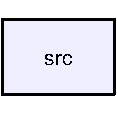
\includegraphics[width=45pt]{dir_000000_dep}
\end{center}
\end{figure}
\subsection*{Files}
\begin{CompactItemize}
\item 
file \hyperlink{Classes_8c}{Classes.c}
\item 
file \hyperlink{Classes_8h}{Classes.h}
\item 
file \hyperlink{Convenience_8c}{Convenience.c}
\item 
file \hyperlink{Convenience_8h}{Convenience.h}
\item 
file \hyperlink{Distributions_8c}{Distributions.c}
\item 
file \hyperlink{Distributions_8h}{Distributions.h}
\item 
file \hyperlink{IndependenceTest_8c}{Independence\-Test.c}
\item 
file \hyperlink{IndependenceTest_8h}{Independence\-Test.h}
\item 
file \hyperlink{LinearStatistic_8c}{Linear\-Statistic.c}
\item 
file \hyperlink{LinearStatistic_8h}{Linear\-Statistic.h}
\item 
file \hyperlink{mvt_8h}{mvt.h}
\item 
file \hyperlink{Node_8c}{Node.c}
\item 
file \hyperlink{Node_8h}{Node.h}
\item 
file \hyperlink{party_8h}{party.h}
\item 
file \hyperlink{Predict_8c}{Predict.c}
\item 
file \hyperlink{Predict_8h}{Predict.h}
\item 
file \hyperlink{randomF77_8c}{random\-F77.c}
\item 
file \hyperlink{S3Classes_8c}{S3Classes.c}
\item 
file \hyperlink{S3Classes_8h}{S3Classes.h}
\item 
file \hyperlink{Splits_8c}{Splits.c}
\item 
file \hyperlink{Splits_8h}{Splits.h}
\item 
file \hyperlink{SurrogateSplits_8c}{Surrogate\-Splits.c}
\item 
file \hyperlink{SurrogateSplits_8h}{Surrogate\-Splits.h}
\item 
file \hyperlink{TestStatistic_8c}{Test\-Statistic.c}
\item 
file \hyperlink{TestStatistic_8h}{Test\-Statistic.h}
\item 
file \hyperlink{TreeGrow_8c}{Tree\-Grow.c}
\item 
file \hyperlink{Utils_8c}{Utils.c}
\item 
file \hyperlink{Utils_8h}{Utils.h}
\end{CompactItemize}

\chapter{party File Documentation}
\hypertarget{Classes_8c}{
\section{Classes.c File Reference}
\label{Classes_8c}\index{Classes.c@{Classes.c}}
}
{\tt \#include \char`\"{}party.h\char`\"{}}\par


Include dependency graph for Classes.c:\begin{figure}[H]
\begin{center}
\leavevmode
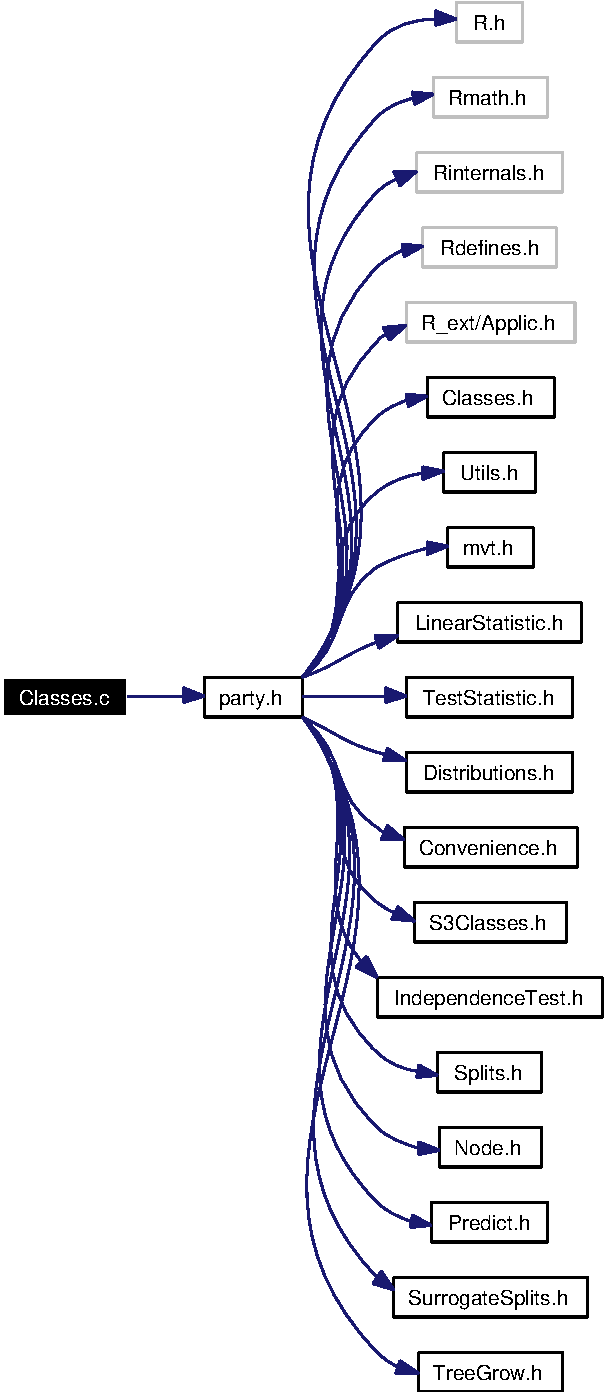
\includegraphics[width=159pt]{Classes_8c__incl}
\end{center}
\end{figure}
\subsection*{Functions}
\begin{CompactItemize}
\item 
SEXP \hyperlink{Classes_8c_a62}{party\_\-init} (void)
\item 
int \hyperlink{Classes_8c_a63}{get\_\-dimension} (SEXP object)
\item 
int \hyperlink{Classes_8c_a64}{get\_\-teststattype} (SEXP object)
\item 
int \hyperlink{Classes_8c_a65}{get\_\-pvalue} (SEXP object)
\item 
double \hyperlink{Classes_8c_a66}{get\_\-tol} (SEXP object)
\item 
int \hyperlink{Classes_8c_a67}{get\_\-maxpts} (SEXP object)
\item 
double \hyperlink{Classes_8c_a68}{get\_\-abseps} (SEXP object)
\item 
double \hyperlink{Classes_8c_a69}{get\_\-releps} (SEXP object)
\item 
double \hyperlink{Classes_8c_a70}{get\_\-minsplit} (SEXP object)
\item 
double \hyperlink{Classes_8c_a71}{get\_\-minprob} (SEXP object)
\item 
double \hyperlink{Classes_8c_a72}{get\_\-minbucket} (SEXP object)
\item 
SEXP \hyperlink{Classes_8c_a73}{get\_\-transformation} (SEXP object, int variable)
\item 
SEXP \hyperlink{Classes_8c_a74}{get\_\-jointtransf} (SEXP object)
\item 
SEXP \hyperlink{Classes_8c_a75}{get\_\-variable} (SEXP object, int variable)
\item 
int \hyperlink{Classes_8c_a76}{is\_\-nominal} (SEXP object, int variable)
\item 
int \hyperlink{Classes_8c_a77}{is\_\-ordinal} (SEXP object, int variable)
\item 
int \hyperlink{Classes_8c_a78}{is\_\-censored} (SEXP object, int variable)
\item 
int \hyperlink{Classes_8c_a79}{has\_\-missings} (SEXP object, int variable)
\item 
SEXP \hyperlink{Classes_8c_a80}{get\_\-ordering} (SEXP object, int variable)
\item 
SEXP \hyperlink{Classes_8c_a81}{get\_\-levels} (SEXP object, int variable)
\item 
SEXP \hyperlink{Classes_8c_a82}{get\_\-scores} (SEXP object, int variable)
\item 
SEXP \hyperlink{Classes_8c_a83}{get\_\-missings} (SEXP object, int variable)
\item 
SEXP \hyperlink{Classes_8c_a84}{get\_\-varmemory} (SEXP object, int variable)
\item 
SEXP \hyperlink{Classes_8c_a85}{get\_\-var\-Mmemory} (SEXP object, int variable)
\item 
SEXP \hyperlink{Classes_8c_a86}{get\_\-Mscorematrix} (SEXP object, int variable)
\item 
int \hyperlink{Classes_8c_a87}{get\_\-savesplitstats} (SEXP object)
\item 
SEXP \hyperlink{Classes_8c_a88}{get\_\-splitstatistics} (SEXP object)
\item 
int \hyperlink{Classes_8c_a89}{get\_\-nobs} (SEXP object)
\item 
int \hyperlink{Classes_8c_a90}{get\_\-ninputs} (SEXP object)
\item 
SEXP \hyperlink{Classes_8c_a91}{get\_\-weights} (SEXP object, int variable)
\item 
int \hyperlink{Classes_8c_a92}{get\_\-testtype} (SEXP object)
\item 
int \hyperlink{Classes_8c_a93}{get\_\-nresample} (SEXP object)
\item 
SEXP \hyperlink{Classes_8c_a94}{get\_\-varctrl} (SEXP object)
\item 
SEXP \hyperlink{Classes_8c_a95}{get\_\-splitctrl} (SEXP object)
\item 
SEXP \hyperlink{Classes_8c_a96}{get\_\-gtctrl} (SEXP object)
\item 
SEXP \hyperlink{Classes_8c_a97}{get\_\-tgctrl} (SEXP object)
\item 
double \hyperlink{Classes_8c_a98}{get\_\-mincriterion} (SEXP object)
\item 
int \hyperlink{Classes_8c_a99}{get\_\-maxsurrogate} (SEXP object)
\item 
int \hyperlink{Classes_8c_a100}{get\_\-randomsplits} (SEXP object)
\item 
int \hyperlink{Classes_8c_a101}{get\_\-mtry} (SEXP object)
\item 
SEXP \hyperlink{Classes_8c_a102}{get\_\-dontuse} (SEXP object)
\item 
SEXP \hyperlink{Classes_8c_a103}{get\_\-dontusetmp} (SEXP object)
\item 
int \hyperlink{Classes_8c_a104}{get\_\-stump} (SEXP object)
\end{CompactItemize}
\subsection*{Variables}
\begin{CompactItemize}
\item 
SEXP \hyperlink{Classes_8c_a0}{PL2\_\-expectation\-Sym}
\item 
SEXP \hyperlink{Classes_8c_a1}{PL2\_\-covariance\-Sym}
\item 
SEXP \hyperlink{Classes_8c_a2}{PL2\_\-linearstatistic\-Sym}
\item 
SEXP \hyperlink{Classes_8c_a3}{PL2\_\-expcovinf\-Sym}
\item 
SEXP \hyperlink{Classes_8c_a4}{PL2\_\-expcovinfss\-Sym}
\item 
SEXP \hyperlink{Classes_8c_a5}{PL2\_\-sumweights\-Sym}
\item 
SEXP \hyperlink{Classes_8c_a6}{PL2\_\-dimension\-Sym}
\item 
SEXP \hyperlink{Classes_8c_a7}{PL2\_\-MPinv\-Sym}
\item 
SEXP \hyperlink{Classes_8c_a8}{PL2\_\-rank\-Sym}
\item 
SEXP \hyperlink{Classes_8c_a9}{PL2\_\-svd\-Sym}
\item 
SEXP \hyperlink{Classes_8c_a10}{PL2\_\-svdmem\-Sym}
\item 
SEXP \hyperlink{Classes_8c_a11}{PL2\_\-method\-Sym}
\item 
SEXP \hyperlink{Classes_8c_a12}{PL2\_\-jobu\-Sym}
\item 
SEXP \hyperlink{Classes_8c_a13}{PL2\_\-jobv\-Sym}
\item 
SEXP \hyperlink{Classes_8c_a14}{PL2\_\-u\-Sym}
\item 
SEXP \hyperlink{Classes_8c_a15}{PL2\_\-v\-Sym}
\item 
SEXP \hyperlink{Classes_8c_a16}{PL2\_\-s\-Sym}
\item 
SEXP \hyperlink{Classes_8c_a17}{PL2\_\-p\-Sym}
\item 
SEXP \hyperlink{Classes_8c_a18}{PL2\_\-teststattype\-Sym}
\item 
SEXP \hyperlink{Classes_8c_a19}{PL2\_\-pvalue\-Sym}
\item 
SEXP \hyperlink{Classes_8c_a20}{PL2\_\-tol\-Sym}
\item 
SEXP \hyperlink{Classes_8c_a21}{PL2\_\-maxpts\-Sym}
\item 
SEXP \hyperlink{Classes_8c_a22}{PL2\_\-abseps\-Sym}
\item 
SEXP \hyperlink{Classes_8c_a23}{PL2\_\-releps\-Sym}
\item 
SEXP \hyperlink{Classes_8c_a24}{PL2\_\-minprob\-Sym}
\item 
SEXP \hyperlink{Classes_8c_a25}{PL2\_\-minsplit\-Sym}
\item 
SEXP \hyperlink{Classes_8c_a26}{PL2\_\-minbucket\-Sym}
\item 
SEXP \hyperlink{Classes_8c_a27}{PL2\_\-variables\-Sym}
\item 
SEXP \hyperlink{Classes_8c_a28}{PL2\_\-transformations\-Sym}
\item 
SEXP \hyperlink{Classes_8c_a29}{PL2\_\-is\_\-nominal\-Sym}
\item 
SEXP \hyperlink{Classes_8c_a30}{PL2\_\-is\_\-ordinal\-Sym}
\item 
SEXP \hyperlink{Classes_8c_a31}{PL2\_\-is\_\-censored\-Sym}
\item 
SEXP \hyperlink{Classes_8c_a32}{PL2\_\-ordering\-Sym}
\item 
SEXP \hyperlink{Classes_8c_a33}{PL2\_\-levels\-Sym}
\item 
SEXP \hyperlink{Classes_8c_a34}{PL2\_\-scores\-Sym}
\item 
SEXP \hyperlink{Classes_8c_a35}{PL2\_\-has\_\-missings\-Sym}
\item 
SEXP \hyperlink{Classes_8c_a36}{PL2\_\-which\-NASym}
\item 
SEXP \hyperlink{Classes_8c_a37}{PL2\_\-jointtransf\-Sym}
\item 
SEXP \hyperlink{Classes_8c_a38}{PL2\_\-nobs\-Sym}
\item 
SEXP \hyperlink{Classes_8c_a39}{PL2\_\-ninputs\-Sym}
\item 
SEXP \hyperlink{Classes_8c_a40}{PL2\_\-linexpcov2sample\-Sym}
\item 
SEXP \hyperlink{Classes_8c_a41}{PL2\_\-weights\-Sym}
\item 
SEXP \hyperlink{Classes_8c_a42}{PL2\_\-varmemory\-Sym}
\item 
SEXP \hyperlink{Classes_8c_a43}{PL2\_\-var\-Mmemory\-Sym}
\item 
SEXP \hyperlink{Classes_8c_a44}{PL2\_\-Mscorematrices\-Sym}
\item 
SEXP \hyperlink{Classes_8c_a45}{PL2\_\-splitstatistics\-Sym}
\item 
SEXP \hyperlink{Classes_8c_a46}{PL2\_\-savesplitstats\-Sym}
\item 
SEXP \hyperlink{Classes_8c_a47}{PL2\_\-responses\-Sym}
\item 
SEXP \hyperlink{Classes_8c_a48}{PL2\_\-inputs\-Sym}
\item 
SEXP \hyperlink{Classes_8c_a49}{PL2\_\-testtype\-Sym}
\item 
SEXP \hyperlink{Classes_8c_a50}{PL2\_\-nresample\-Sym}
\item 
SEXP \hyperlink{Classes_8c_a51}{PL2\_\-varctrl\-Sym}
\item 
SEXP \hyperlink{Classes_8c_a52}{PL2\_\-splitctrl\-Sym}
\item 
SEXP \hyperlink{Classes_8c_a53}{PL2\_\-gtctrl\-Sym}
\item 
SEXP \hyperlink{Classes_8c_a54}{PL2\_\-mincriterion\-Sym}
\item 
SEXP \hyperlink{Classes_8c_a55}{PL2\_\-maxsurrogate\-Sym}
\item 
SEXP \hyperlink{Classes_8c_a56}{PL2\_\-randomsplits\-Sym}
\item 
SEXP \hyperlink{Classes_8c_a57}{PL2\_\-mtry\-Sym}
\item 
SEXP \hyperlink{Classes_8c_a58}{PL2\_\-dontuse\-Sym}
\item 
SEXP \hyperlink{Classes_8c_a59}{PL2\_\-dontusetmp\-Sym}
\item 
SEXP \hyperlink{Classes_8c_a60}{PL2\_\-stump\-Sym}
\item 
SEXP \hyperlink{Classes_8c_a61}{PL2\_\-tgctrl\-Sym}
\end{CompactItemize}


\subsection{Detailed Description}
S4 classes for package `party'

\begin{Desc}
\item[Author:]\begin{Desc}
\item[Author]hothorn \end{Desc}
\end{Desc}
\begin{Desc}
\item[Date:]\begin{Desc}
\item[Date]2005/06/14 09:21:32 \end{Desc}
\end{Desc}


Definition in file \hyperlink{Classes_8c-source}{Classes.c}.

\subsection{Function Documentation}
\hypertarget{Classes_8c_a68}{
\index{Classes.c@{Classes.c}!get_abseps@{get\_\-abseps}}
\index{get_abseps@{get\_\-abseps}!Classes.c@{Classes.c}}
\subsubsection[get\_\-abseps]{\setlength{\rightskip}{0pt plus 5cm}double get\_\-abseps (SEXP {\em object})}}
\label{Classes_8c_a68}




Definition at line 163 of file Classes.c.

References PL2\_\-abseps\-Sym.

Referenced by C\_\-Teststat\-Pvalue().\hypertarget{Classes_8c_a63}{
\index{Classes.c@{Classes.c}!get_dimension@{get\_\-dimension}}
\index{get_dimension@{get\_\-dimension}!Classes.c@{Classes.c}}
\subsubsection[get\_\-dimension]{\setlength{\rightskip}{0pt plus 5cm}int get\_\-dimension (SEXP {\em object})}}
\label{Classes_8c_a63}




Definition at line 143 of file Classes.c.

References PL2\_\-dimension\-Sym.

Referenced by C\_\-Conditional\-Pvalue(), C\_\-MLinear\-Statistic(), C\_\-Node(), C\_\-Test\-Statistic(), and R\_\-splitcategorical().\hypertarget{Classes_8c_a102}{
\index{Classes.c@{Classes.c}!get_dontuse@{get\_\-dontuse}}
\index{get_dontuse@{get\_\-dontuse}!Classes.c@{Classes.c}}
\subsubsection[get\_\-dontuse]{\setlength{\rightskip}{0pt plus 5cm}SEXP get\_\-dontuse (SEXP {\em object})}}
\label{Classes_8c_a102}




Definition at line 335 of file Classes.c.

References PL2\_\-dontuse\-Sym.

Referenced by C\_\-Global\-Test().\hypertarget{Classes_8c_a103}{
\index{Classes.c@{Classes.c}!get_dontusetmp@{get\_\-dontusetmp}}
\index{get_dontusetmp@{get\_\-dontusetmp}!Classes.c@{Classes.c}}
\subsubsection[get\_\-dontusetmp]{\setlength{\rightskip}{0pt plus 5cm}SEXP get\_\-dontusetmp (SEXP {\em object})}}
\label{Classes_8c_a103}




Definition at line 339 of file Classes.c.

References PL2\_\-dontusetmp\-Sym.

Referenced by C\_\-Global\-Test().\hypertarget{Classes_8c_a96}{
\index{Classes.c@{Classes.c}!get_gtctrl@{get\_\-gtctrl}}
\index{get_gtctrl@{get\_\-gtctrl}!Classes.c@{Classes.c}}
\subsubsection[get\_\-gtctrl]{\setlength{\rightskip}{0pt plus 5cm}SEXP get\_\-gtctrl (SEXP {\em object})}}
\label{Classes_8c_a96}




Definition at line 311 of file Classes.c.

References PL2\_\-gtctrl\-Sym.

Referenced by C\_\-Node().\hypertarget{Classes_8c_a74}{
\index{Classes.c@{Classes.c}!get_jointtransf@{get\_\-jointtransf}}
\index{get_jointtransf@{get\_\-jointtransf}!Classes.c@{Classes.c}}
\subsubsection[get\_\-jointtransf]{\setlength{\rightskip}{0pt plus 5cm}SEXP get\_\-jointtransf (SEXP {\em object})}}
\label{Classes_8c_a74}




Definition at line 189 of file Classes.c.

References PL2\_\-jointtransf\-Sym.\hypertarget{Classes_8c_a81}{
\index{Classes.c@{Classes.c}!get_levels@{get\_\-levels}}
\index{get_levels@{get\_\-levels}!Classes.c@{Classes.c}}
\subsubsection[get\_\-levels]{\setlength{\rightskip}{0pt plus 5cm}SEXP get\_\-levels (SEXP {\em object}, int {\em variable})}}
\label{Classes_8c_a81}




Definition at line 226 of file Classes.c.

References is\_\-nominal(), is\_\-ordinal(), and PL2\_\-levels\-Sym.

Referenced by C\_\-Node().

Here is the call graph for this function:\begin{figure}[H]
\begin{center}
\leavevmode
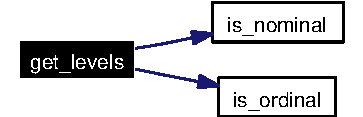
\includegraphics[width=104pt]{Classes_8c_a81_cgraph}
\end{center}
\end{figure}
\hypertarget{Classes_8c_a67}{
\index{Classes.c@{Classes.c}!get_maxpts@{get\_\-maxpts}}
\index{get_maxpts@{get\_\-maxpts}!Classes.c@{Classes.c}}
\subsubsection[get\_\-maxpts]{\setlength{\rightskip}{0pt plus 5cm}int get\_\-maxpts (SEXP {\em object})}}
\label{Classes_8c_a67}




Definition at line 159 of file Classes.c.

References PL2\_\-maxpts\-Sym.

Referenced by C\_\-Teststat\-Pvalue().\hypertarget{Classes_8c_a99}{
\index{Classes.c@{Classes.c}!get_maxsurrogate@{get\_\-maxsurrogate}}
\index{get_maxsurrogate@{get\_\-maxsurrogate}!Classes.c@{Classes.c}}
\subsubsection[get\_\-maxsurrogate]{\setlength{\rightskip}{0pt plus 5cm}int get\_\-maxsurrogate (SEXP {\em object})}}
\label{Classes_8c_a99}




Definition at line 323 of file Classes.c.

References PL2\_\-maxsurrogate\-Sym.

Referenced by C\_\-splitnode(), C\_\-surrogates(), C\_\-Tree\-Grow(), R\_\-Ensemble(), R\_\-Node(), and R\_\-Tree\-Grow().\hypertarget{Classes_8c_a72}{
\index{Classes.c@{Classes.c}!get_minbucket@{get\_\-minbucket}}
\index{get_minbucket@{get\_\-minbucket}!Classes.c@{Classes.c}}
\subsubsection[get\_\-minbucket]{\setlength{\rightskip}{0pt plus 5cm}double get\_\-minbucket (SEXP {\em object})}}
\label{Classes_8c_a72}




Definition at line 179 of file Classes.c.

References PL2\_\-minbucket\-Sym.

Referenced by C\_\-split().\hypertarget{Classes_8c_a98}{
\index{Classes.c@{Classes.c}!get_mincriterion@{get\_\-mincriterion}}
\index{get_mincriterion@{get\_\-mincriterion}!Classes.c@{Classes.c}}
\subsubsection[get\_\-mincriterion]{\setlength{\rightskip}{0pt plus 5cm}double get\_\-mincriterion (SEXP {\em object})}}
\label{Classes_8c_a98}




Definition at line 319 of file Classes.c.

References PL2\_\-mincriterion\-Sym.

Referenced by C\_\-Node().\hypertarget{Classes_8c_a71}{
\index{Classes.c@{Classes.c}!get_minprob@{get\_\-minprob}}
\index{get_minprob@{get\_\-minprob}!Classes.c@{Classes.c}}
\subsubsection[get\_\-minprob]{\setlength{\rightskip}{0pt plus 5cm}double get\_\-minprob (SEXP {\em object})}}
\label{Classes_8c_a71}




Definition at line 175 of file Classes.c.

References PL2\_\-minprob\-Sym.

Referenced by C\_\-split().\hypertarget{Classes_8c_a70}{
\index{Classes.c@{Classes.c}!get_minsplit@{get\_\-minsplit}}
\index{get_minsplit@{get\_\-minsplit}!Classes.c@{Classes.c}}
\subsubsection[get\_\-minsplit]{\setlength{\rightskip}{0pt plus 5cm}double get\_\-minsplit (SEXP {\em object})}}
\label{Classes_8c_a70}




Definition at line 171 of file Classes.c.

References PL2\_\-minsplit\-Sym.

Referenced by C\_\-Node().\hypertarget{Classes_8c_a83}{
\index{Classes.c@{Classes.c}!get_missings@{get\_\-missings}}
\index{get_missings@{get\_\-missings}!Classes.c@{Classes.c}}
\subsubsection[get\_\-missings]{\setlength{\rightskip}{0pt plus 5cm}SEXP get\_\-missings (SEXP {\em object}, int {\em variable})}}
\label{Classes_8c_a83}




Definition at line 249 of file Classes.c.

References has\_\-missings(), and PL2\_\-which\-NASym.

Referenced by C\_\-get\_\-node(), C\_\-Global\-Test(), C\_\-splitnode(), C\_\-splitsurrogate(), and C\_\-surrogates().

Here is the call graph for this function:\begin{figure}[H]
\begin{center}
\leavevmode
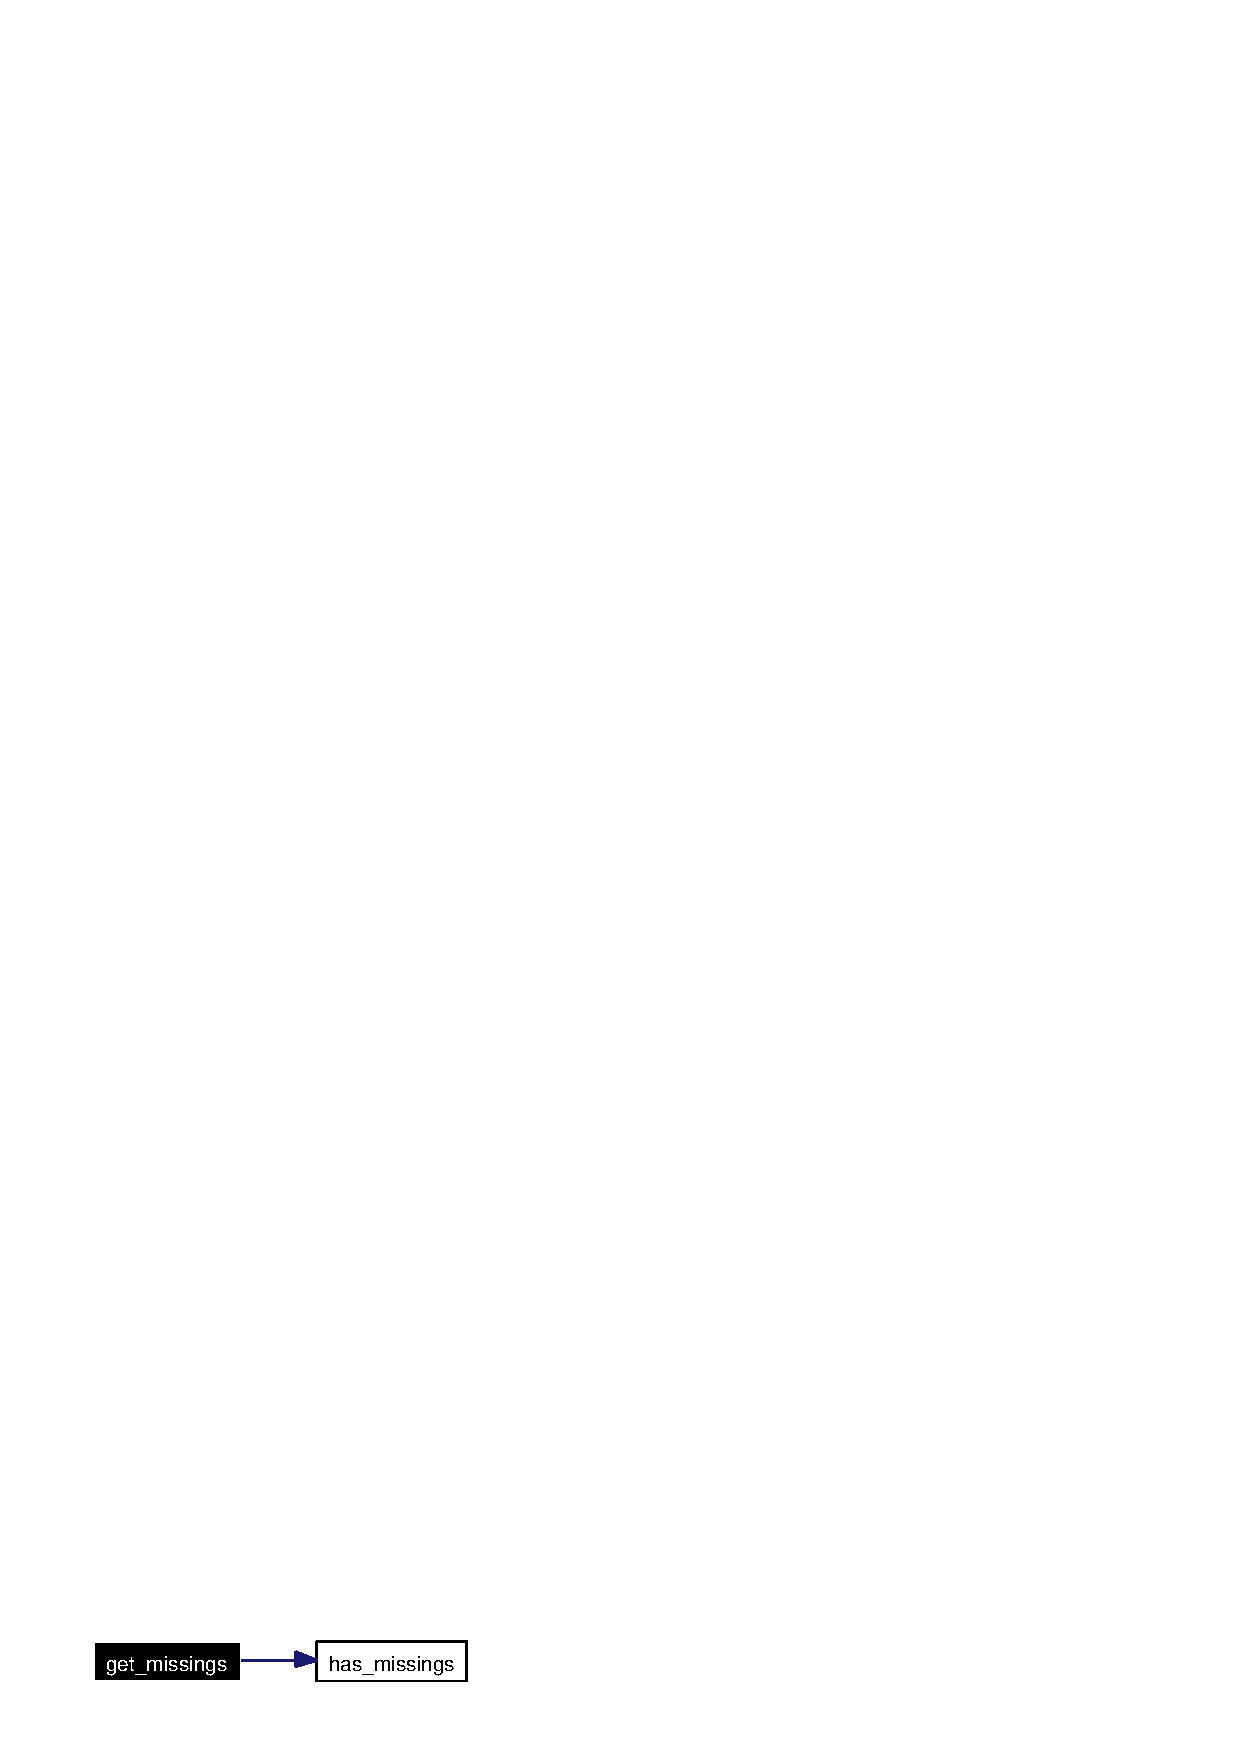
\includegraphics[width=116pt]{Classes_8c_a83_cgraph}
\end{center}
\end{figure}
\hypertarget{Classes_8c_a86}{
\index{Classes.c@{Classes.c}!get_Mscorematrix@{get\_\-Mscorematrix}}
\index{get_Mscorematrix@{get\_\-Mscorematrix}!Classes.c@{Classes.c}}
\subsubsection[get\_\-Mscorematrix]{\setlength{\rightskip}{0pt plus 5cm}SEXP get\_\-Mscorematrix (SEXP {\em object}, int {\em variable})}}
\label{Classes_8c_a86}




Definition at line 270 of file Classes.c.

References PL2\_\-Mscorematrices\-Sym.

Referenced by C\_\-Global\-Test(), and C\_\-Monte\-Carlo().\hypertarget{Classes_8c_a101}{
\index{Classes.c@{Classes.c}!get_mtry@{get\_\-mtry}}
\index{get_mtry@{get\_\-mtry}!Classes.c@{Classes.c}}
\subsubsection[get\_\-mtry]{\setlength{\rightskip}{0pt plus 5cm}int get\_\-mtry (SEXP {\em object})}}
\label{Classes_8c_a101}




Definition at line 331 of file Classes.c.

References PL2\_\-mtry\-Sym.

Referenced by C\_\-Global\-Test().\hypertarget{Classes_8c_a90}{
\index{Classes.c@{Classes.c}!get_ninputs@{get\_\-ninputs}}
\index{get_ninputs@{get\_\-ninputs}!Classes.c@{Classes.c}}
\subsubsection[get\_\-ninputs]{\setlength{\rightskip}{0pt plus 5cm}int get\_\-ninputs (SEXP {\em object})}}
\label{Classes_8c_a90}




Definition at line 287 of file Classes.c.

References PL2\_\-ninputs\-Sym.

Referenced by C\_\-Global\-Test(), C\_\-Monte\-Carlo(), C\_\-Node(), C\_\-splitnode(), C\_\-surrogates(), R\_\-Ensemble(), R\_\-Global\-Test(), R\_\-Monte\-Carlo(), R\_\-Node(), and R\_\-Tree\-Grow().\hypertarget{Classes_8c_a89}{
\index{Classes.c@{Classes.c}!get_nobs@{get\_\-nobs}}
\index{get_nobs@{get\_\-nobs}!Classes.c@{Classes.c}}
\subsubsection[get\_\-nobs]{\setlength{\rightskip}{0pt plus 5cm}int get\_\-nobs (SEXP {\em object})}}
\label{Classes_8c_a89}




Definition at line 283 of file Classes.c.

References PL2\_\-nobs\-Sym.

Referenced by C\_\-Global\-Test(), C\_\-Monte\-Carlo(), C\_\-Node(), C\_\-predict(), C\_\-splitnode(), C\_\-splitsurrogate(), C\_\-surrogates(), C\_\-Tree\-Grow(), C\_\-weights(), R\_\-Ensemble(), R\_\-get\_\-node\-ID(), R\_\-Node(), R\_\-predict(), R\_\-predict\-RF(), R\_\-predict\-RF2(), R\_\-Tree\-Grow(), and R\_\-weights().\hypertarget{Classes_8c_a93}{
\index{Classes.c@{Classes.c}!get_nresample@{get\_\-nresample}}
\index{get_nresample@{get\_\-nresample}!Classes.c@{Classes.c}}
\subsubsection[get\_\-nresample]{\setlength{\rightskip}{0pt plus 5cm}int get\_\-nresample (SEXP {\em object})}}
\label{Classes_8c_a93}




Definition at line 299 of file Classes.c.

References PL2\_\-nresample\-Sym.

Referenced by C\_\-Monte\-Carlo().\hypertarget{Classes_8c_a80}{
\index{Classes.c@{Classes.c}!get_ordering@{get\_\-ordering}}
\index{get_ordering@{get\_\-ordering}!Classes.c@{Classes.c}}
\subsubsection[get\_\-ordering]{\setlength{\rightskip}{0pt plus 5cm}SEXP get\_\-ordering (SEXP {\em object}, int {\em variable})}}
\label{Classes_8c_a80}




Definition at line 215 of file Classes.c.

References is\_\-nominal(), and PL2\_\-ordering\-Sym.

Referenced by C\_\-Node(), and C\_\-surrogates().

Here is the call graph for this function:\begin{figure}[H]
\begin{center}
\leavevmode
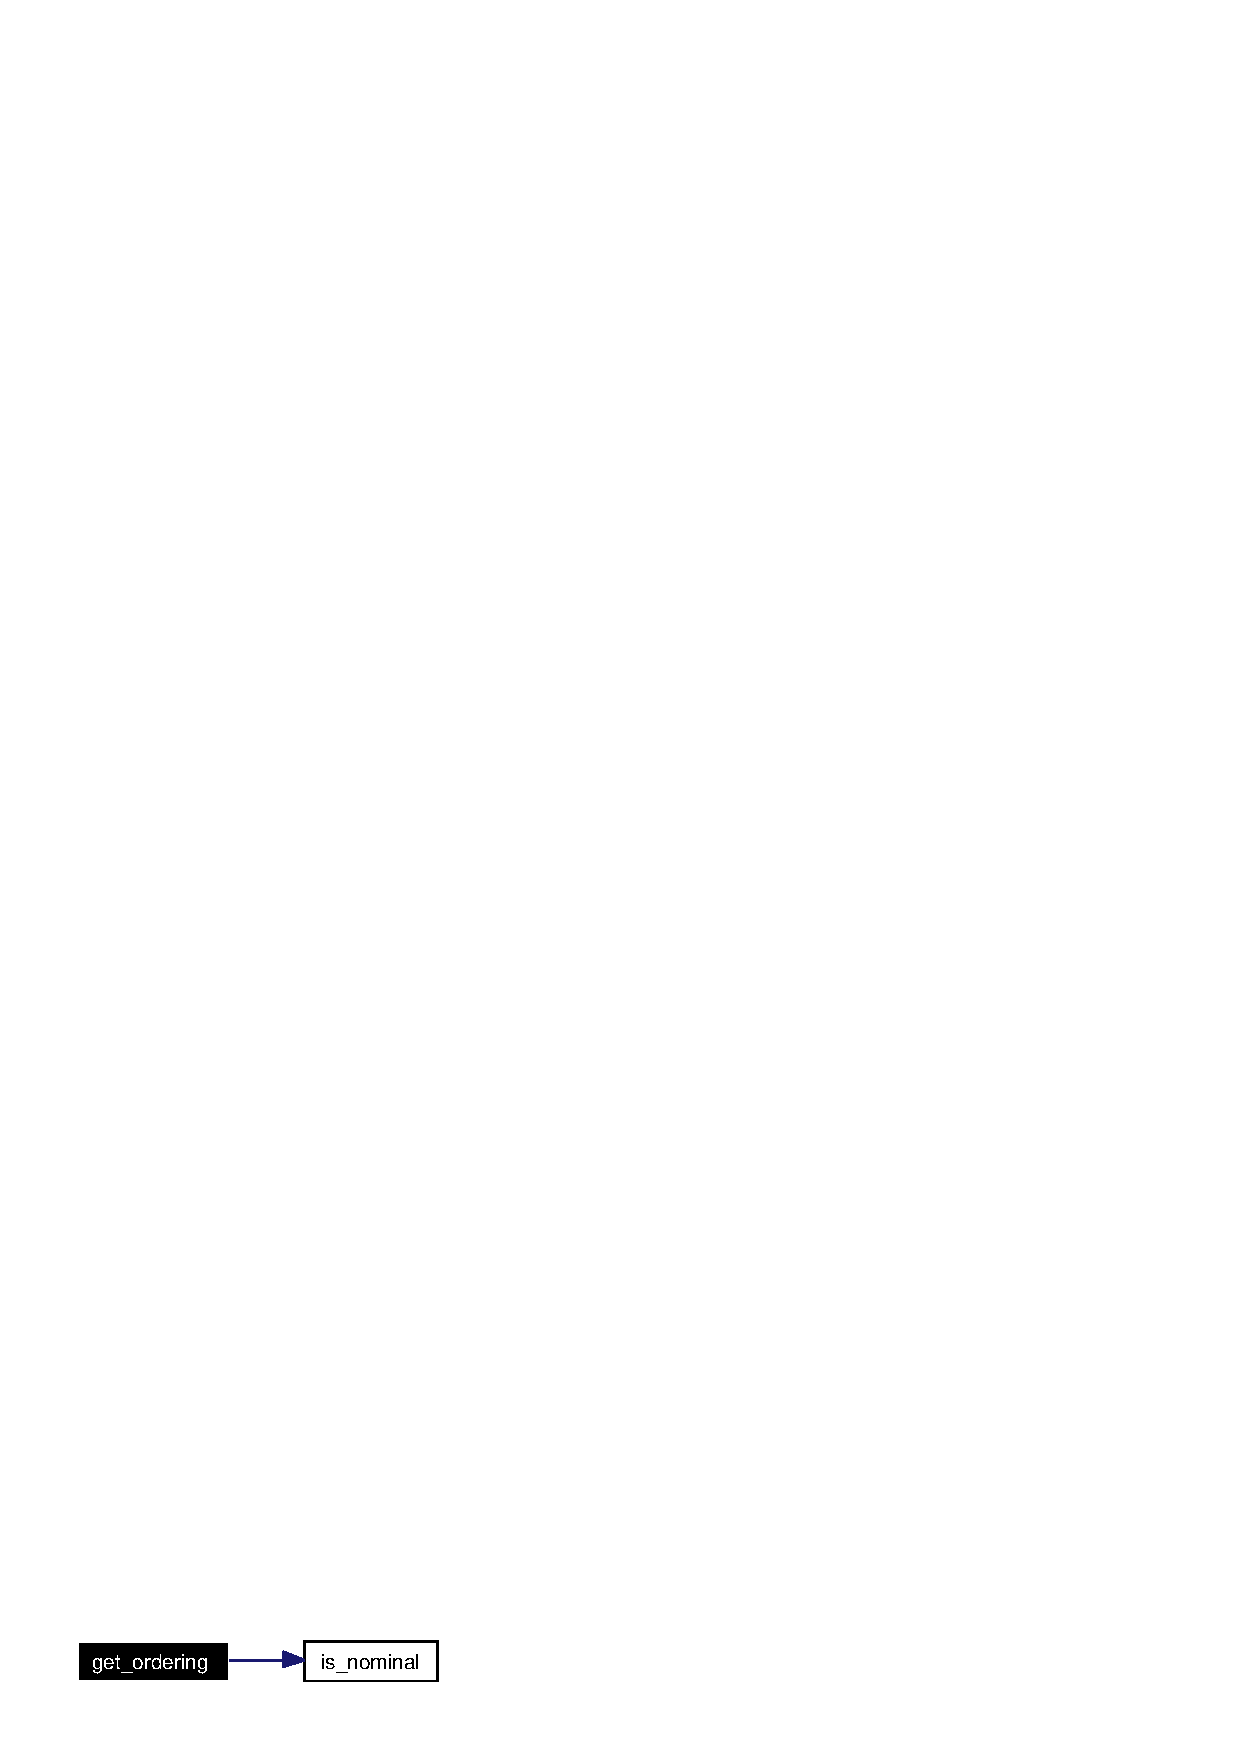
\includegraphics[width=112pt]{Classes_8c_a80_cgraph}
\end{center}
\end{figure}
\hypertarget{Classes_8c_a65}{
\index{Classes.c@{Classes.c}!get_pvalue@{get\_\-pvalue}}
\index{get_pvalue@{get\_\-pvalue}!Classes.c@{Classes.c}}
\subsubsection[get\_\-pvalue]{\setlength{\rightskip}{0pt plus 5cm}int get\_\-pvalue (SEXP {\em object})}}
\label{Classes_8c_a65}




Definition at line 151 of file Classes.c.

References PL2\_\-pvalue\-Sym.

Referenced by C\_\-Teststat\-Criterion(), and C\_\-Teststat\-Pvalue().\hypertarget{Classes_8c_a100}{
\index{Classes.c@{Classes.c}!get_randomsplits@{get\_\-randomsplits}}
\index{get_randomsplits@{get\_\-randomsplits}!Classes.c@{Classes.c}}
\subsubsection[get\_\-randomsplits]{\setlength{\rightskip}{0pt plus 5cm}int get\_\-randomsplits (SEXP {\em object})}}
\label{Classes_8c_a100}




Definition at line 327 of file Classes.c.

References PL2\_\-randomsplits\-Sym.

Referenced by C\_\-Global\-Test().\hypertarget{Classes_8c_a69}{
\index{Classes.c@{Classes.c}!get_releps@{get\_\-releps}}
\index{get_releps@{get\_\-releps}!Classes.c@{Classes.c}}
\subsubsection[get\_\-releps]{\setlength{\rightskip}{0pt plus 5cm}double get\_\-releps (SEXP {\em object})}}
\label{Classes_8c_a69}




Definition at line 167 of file Classes.c.

References PL2\_\-releps\-Sym.

Referenced by C\_\-Teststat\-Pvalue().\hypertarget{Classes_8c_a87}{
\index{Classes.c@{Classes.c}!get_savesplitstats@{get\_\-savesplitstats}}
\index{get_savesplitstats@{get\_\-savesplitstats}!Classes.c@{Classes.c}}
\subsubsection[get\_\-savesplitstats]{\setlength{\rightskip}{0pt plus 5cm}int get\_\-savesplitstats (SEXP {\em object})}}
\label{Classes_8c_a87}




Definition at line 275 of file Classes.c.

References PL2\_\-savesplitstats\-Sym.

Referenced by C\_\-Node().\hypertarget{Classes_8c_a82}{
\index{Classes.c@{Classes.c}!get_scores@{get\_\-scores}}
\index{get_scores@{get\_\-scores}!Classes.c@{Classes.c}}
\subsubsection[get\_\-scores]{\setlength{\rightskip}{0pt plus 5cm}SEXP get\_\-scores (SEXP {\em object}, int {\em variable})}}
\label{Classes_8c_a82}




Definition at line 238 of file Classes.c.

References is\_\-ordinal(), and PL2\_\-scores\-Sym.

Here is the call graph for this function:\begin{figure}[H]
\begin{center}
\leavevmode
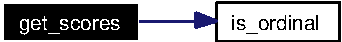
\includegraphics[width=101pt]{Classes_8c_a82_cgraph}
\end{center}
\end{figure}
\hypertarget{Classes_8c_a95}{
\index{Classes.c@{Classes.c}!get_splitctrl@{get\_\-splitctrl}}
\index{get_splitctrl@{get\_\-splitctrl}!Classes.c@{Classes.c}}
\subsubsection[get\_\-splitctrl]{\setlength{\rightskip}{0pt plus 5cm}SEXP get\_\-splitctrl (SEXP {\em object})}}
\label{Classes_8c_a95}




Definition at line 307 of file Classes.c.

References PL2\_\-splitctrl\-Sym.

Referenced by C\_\-Node(), C\_\-splitnode(), C\_\-surrogates(), C\_\-Tree\-Grow(), R\_\-Ensemble(), R\_\-Node(), and R\_\-Tree\-Grow().\hypertarget{Classes_8c_a88}{
\index{Classes.c@{Classes.c}!get_splitstatistics@{get\_\-splitstatistics}}
\index{get_splitstatistics@{get\_\-splitstatistics}!Classes.c@{Classes.c}}
\subsubsection[get\_\-splitstatistics]{\setlength{\rightskip}{0pt plus 5cm}SEXP get\_\-splitstatistics (SEXP {\em object})}}
\label{Classes_8c_a88}




Definition at line 279 of file Classes.c.

References PL2\_\-splitstatistics\-Sym.

Referenced by C\_\-Node(), and C\_\-surrogates().\hypertarget{Classes_8c_a104}{
\index{Classes.c@{Classes.c}!get_stump@{get\_\-stump}}
\index{get_stump@{get\_\-stump}!Classes.c@{Classes.c}}
\subsubsection[get\_\-stump]{\setlength{\rightskip}{0pt plus 5cm}int get\_\-stump (SEXP {\em object})}}
\label{Classes_8c_a104}




Definition at line 343 of file Classes.c.

References PL2\_\-stump\-Sym.

Referenced by C\_\-Tree\-Grow().\hypertarget{Classes_8c_a64}{
\index{Classes.c@{Classes.c}!get_teststattype@{get\_\-teststattype}}
\index{get_teststattype@{get\_\-teststattype}!Classes.c@{Classes.c}}
\subsubsection[get\_\-teststattype]{\setlength{\rightskip}{0pt plus 5cm}int get\_\-teststattype (SEXP {\em object})}}
\label{Classes_8c_a64}




Definition at line 147 of file Classes.c.

References PL2\_\-teststattype\-Sym.

Referenced by C\_\-Global\-Test(), C\_\-Independence\-Test(), and C\_\-Teststat\-Pvalue().\hypertarget{Classes_8c_a92}{
\index{Classes.c@{Classes.c}!get_testtype@{get\_\-testtype}}
\index{get_testtype@{get\_\-testtype}!Classes.c@{Classes.c}}
\subsubsection[get\_\-testtype]{\setlength{\rightskip}{0pt plus 5cm}int get\_\-testtype (SEXP {\em object})}}
\label{Classes_8c_a92}




Definition at line 295 of file Classes.c.

References PL2\_\-testtype\-Sym.

Referenced by C\_\-Global\-Test().\hypertarget{Classes_8c_a97}{
\index{Classes.c@{Classes.c}!get_tgctrl@{get\_\-tgctrl}}
\index{get_tgctrl@{get\_\-tgctrl}!Classes.c@{Classes.c}}
\subsubsection[get\_\-tgctrl]{\setlength{\rightskip}{0pt plus 5cm}SEXP get\_\-tgctrl (SEXP {\em object})}}
\label{Classes_8c_a97}




Definition at line 315 of file Classes.c.

References PL2\_\-tgctrl\-Sym.

Referenced by C\_\-Node(), and C\_\-Tree\-Grow().\hypertarget{Classes_8c_a66}{
\index{Classes.c@{Classes.c}!get_tol@{get\_\-tol}}
\index{get_tol@{get\_\-tol}!Classes.c@{Classes.c}}
\subsubsection[get\_\-tol]{\setlength{\rightskip}{0pt plus 5cm}double get\_\-tol (SEXP {\em object})}}
\label{Classes_8c_a66}




Definition at line 155 of file Classes.c.

References PL2\_\-tol\-Sym.

Referenced by C\_\-Global\-Test(), C\_\-Independence\-Test(), C\_\-Node(), C\_\-split(), C\_\-splitcategorical(), C\_\-Teststat\-Pvalue(), and R\_\-splitcategorical().\hypertarget{Classes_8c_a73}{
\index{Classes.c@{Classes.c}!get_transformation@{get\_\-transformation}}
\index{get_transformation@{get\_\-transformation}!Classes.c@{Classes.c}}
\subsubsection[get\_\-transformation]{\setlength{\rightskip}{0pt plus 5cm}SEXP get\_\-transformation (SEXP {\em object}, int {\em variable})}}
\label{Classes_8c_a73}




Definition at line 183 of file Classes.c.

References PL2\_\-transformations\-Sym.

Referenced by C\_\-Global\-Test(), C\_\-Monte\-Carlo(), and C\_\-Node().\hypertarget{Classes_8c_a94}{
\index{Classes.c@{Classes.c}!get_varctrl@{get\_\-varctrl}}
\index{get_varctrl@{get\_\-varctrl}!Classes.c@{Classes.c}}
\subsubsection[get\_\-varctrl]{\setlength{\rightskip}{0pt plus 5cm}SEXP get\_\-varctrl (SEXP {\em object})}}
\label{Classes_8c_a94}




Definition at line 303 of file Classes.c.

References PL2\_\-varctrl\-Sym.

Referenced by C\_\-Node().\hypertarget{Classes_8c_a75}{
\index{Classes.c@{Classes.c}!get_variable@{get\_\-variable}}
\index{get_variable@{get\_\-variable}!Classes.c@{Classes.c}}
\subsubsection[get\_\-variable]{\setlength{\rightskip}{0pt plus 5cm}SEXP get\_\-variable (SEXP {\em object}, int {\em variable})}}
\label{Classes_8c_a75}




Definition at line 193 of file Classes.c.

References PL2\_\-variables\-Sym.

Referenced by C\_\-get\_\-node(), C\_\-Node(), C\_\-splitnode(), C\_\-splitsurrogate(), and C\_\-surrogates().\hypertarget{Classes_8c_a84}{
\index{Classes.c@{Classes.c}!get_varmemory@{get\_\-varmemory}}
\index{get_varmemory@{get\_\-varmemory}!Classes.c@{Classes.c}}
\subsubsection[get\_\-varmemory]{\setlength{\rightskip}{0pt plus 5cm}SEXP get\_\-varmemory (SEXP {\em object}, int {\em variable})}}
\label{Classes_8c_a84}




Definition at line 260 of file Classes.c.

References PL2\_\-varmemory\-Sym.

Referenced by C\_\-Global\-Test(), C\_\-Monte\-Carlo(), and C\_\-Node().\hypertarget{Classes_8c_a85}{
\index{Classes.c@{Classes.c}!get_varMmemory@{get\_\-varMmemory}}
\index{get_varMmemory@{get\_\-varMmemory}!Classes.c@{Classes.c}}
\subsubsection[get\_\-varMmemory]{\setlength{\rightskip}{0pt plus 5cm}SEXP get\_\-var\-Mmemory (SEXP {\em object}, int {\em variable})}}
\label{Classes_8c_a85}




Definition at line 265 of file Classes.c.

References PL2\_\-var\-Mmemory\-Sym.

Referenced by C\_\-Global\-Test(), and C\_\-Monte\-Carlo().\hypertarget{Classes_8c_a91}{
\index{Classes.c@{Classes.c}!get_weights@{get\_\-weights}}
\index{get_weights@{get\_\-weights}!Classes.c@{Classes.c}}
\subsubsection[get\_\-weights]{\setlength{\rightskip}{0pt plus 5cm}SEXP get\_\-weights (SEXP {\em object}, int {\em variable})}}
\label{Classes_8c_a91}




Definition at line 291 of file Classes.c.

References PL2\_\-weights\-Sym.

Referenced by C\_\-Global\-Test(), C\_\-Node(), and C\_\-surrogates().\hypertarget{Classes_8c_a79}{
\index{Classes.c@{Classes.c}!has_missings@{has\_\-missings}}
\index{has_missings@{has\_\-missings}!Classes.c@{Classes.c}}
\subsubsection[has\_\-missings]{\setlength{\rightskip}{0pt plus 5cm}int has\_\-missings (SEXP {\em object}, int {\em variable})}}
\label{Classes_8c_a79}




Definition at line 211 of file Classes.c.

References PL2\_\-has\_\-missings\-Sym.

Referenced by C\_\-get\_\-node(), C\_\-Global\-Test(), C\_\-Monte\-Carlo(), C\_\-Node(), C\_\-splitnode(), C\_\-splitsurrogate(), C\_\-surrogates(), and get\_\-missings().\hypertarget{Classes_8c_a78}{
\index{Classes.c@{Classes.c}!is_censored@{is\_\-censored}}
\index{is_censored@{is\_\-censored}!Classes.c@{Classes.c}}
\subsubsection[is\_\-censored]{\setlength{\rightskip}{0pt plus 5cm}int is\_\-censored (SEXP {\em object}, int {\em variable})}}
\label{Classes_8c_a78}




Definition at line 207 of file Classes.c.

References PL2\_\-is\_\-censored\-Sym.\hypertarget{Classes_8c_a76}{
\index{Classes.c@{Classes.c}!is_nominal@{is\_\-nominal}}
\index{is_nominal@{is\_\-nominal}!Classes.c@{Classes.c}}
\subsubsection[is\_\-nominal]{\setlength{\rightskip}{0pt plus 5cm}int is\_\-nominal (SEXP {\em object}, int {\em variable})}}
\label{Classes_8c_a76}




Definition at line 199 of file Classes.c.

References PL2\_\-is\_\-nominal\-Sym.

Referenced by C\_\-Node(), C\_\-surrogates(), get\_\-levels(), and get\_\-ordering().\hypertarget{Classes_8c_a77}{
\index{Classes.c@{Classes.c}!is_ordinal@{is\_\-ordinal}}
\index{is_ordinal@{is\_\-ordinal}!Classes.c@{Classes.c}}
\subsubsection[is\_\-ordinal]{\setlength{\rightskip}{0pt plus 5cm}int is\_\-ordinal (SEXP {\em object}, int {\em variable})}}
\label{Classes_8c_a77}




Definition at line 203 of file Classes.c.

References PL2\_\-is\_\-ordinal\-Sym.

Referenced by C\_\-Global\-Test(), C\_\-Monte\-Carlo(), C\_\-Node(), get\_\-levels(), and get\_\-scores().\hypertarget{Classes_8c_a62}{
\index{Classes.c@{Classes.c}!party_init@{party\_\-init}}
\index{party_init@{party\_\-init}!Classes.c@{Classes.c}}
\subsubsection[party\_\-init]{\setlength{\rightskip}{0pt plus 5cm}SEXP party\_\-init (void)}}
\label{Classes_8c_a62}




Definition at line 75 of file Classes.c.

References PL2\_\-abseps\-Sym, PL2\_\-covariance\-Sym, PL2\_\-dimension\-Sym, PL2\_\-dontuse\-Sym, PL2\_\-dontusetmp\-Sym, PL2\_\-expcovinfss\-Sym, PL2\_\-expcovinf\-Sym, PL2\_\-expectation\-Sym, PL2\_\-gtctrl\-Sym, PL2\_\-has\_\-missings\-Sym, PL2\_\-inputs\-Sym, PL2\_\-is\_\-censored\-Sym, PL2\_\-is\_\-nominal\-Sym, PL2\_\-is\_\-ordinal\-Sym, PL2\_\-jobu\-Sym, PL2\_\-jobv\-Sym, PL2\_\-jointtransf\-Sym, PL2\_\-levels\-Sym, PL2\_\-linearstatistic\-Sym, PL2\_\-linexpcov2sample\-Sym, PL2\_\-maxpts\-Sym, PL2\_\-maxsurrogate\-Sym, PL2\_\-method\-Sym, PL2\_\-minbucket\-Sym, PL2\_\-mincriterion\-Sym, PL2\_\-minprob\-Sym, PL2\_\-minsplit\-Sym, PL2\_\-MPinv\-Sym, PL2\_\-Mscorematrices\-Sym, PL2\_\-mtry\-Sym, PL2\_\-ninputs\-Sym, PL2\_\-nobs\-Sym, PL2\_\-nresample\-Sym, PL2\_\-ordering\-Sym, PL2\_\-p\-Sym, PL2\_\-pvalue\-Sym, PL2\_\-randomsplits\-Sym, PL2\_\-rank\-Sym, PL2\_\-releps\-Sym, PL2\_\-responses\-Sym, PL2\_\-savesplitstats\-Sym, PL2\_\-scores\-Sym, PL2\_\-splitctrl\-Sym, PL2\_\-splitstatistics\-Sym, PL2\_\-s\-Sym, PL2\_\-stump\-Sym, PL2\_\-sumweights\-Sym, PL2\_\-svdmem\-Sym, PL2\_\-svd\-Sym, PL2\_\-teststattype\-Sym, PL2\_\-testtype\-Sym, PL2\_\-tgctrl\-Sym, PL2\_\-tol\-Sym, PL2\_\-transformations\-Sym, PL2\_\-u\-Sym, PL2\_\-varctrl\-Sym, PL2\_\-variables\-Sym, PL2\_\-varmemory\-Sym, PL2\_\-var\-Mmemory\-Sym, PL2\_\-v\-Sym, PL2\_\-weights\-Sym, and PL2\_\-which\-NASym.

\subsection{Variable Documentation}
\hypertarget{Classes_8c_a22}{
\index{Classes.c@{Classes.c}!PL2_absepsSym@{PL2\_\-absepsSym}}
\index{PL2_absepsSym@{PL2\_\-absepsSym}!Classes.c@{Classes.c}}
\subsubsection[PL2\_\-absepsSym]{\setlength{\rightskip}{0pt plus 5cm}SEXP \hyperlink{Classes_8h_a22}{PL2\_\-abseps\-Sym}}}
\label{Classes_8c_a22}




Definition at line 12 of file Classes.c.

Referenced by get\_\-abseps(), and party\_\-init().\hypertarget{Classes_8c_a1}{
\index{Classes.c@{Classes.c}!PL2_covarianceSym@{PL2\_\-covarianceSym}}
\index{PL2_covarianceSym@{PL2\_\-covarianceSym}!Classes.c@{Classes.c}}
\subsubsection[PL2\_\-covarianceSym]{\setlength{\rightskip}{0pt plus 5cm}SEXP \hyperlink{Classes_8h_a1}{PL2\_\-covariance\-Sym}}}
\label{Classes_8c_a1}




Definition at line 12 of file Classes.c.

Referenced by C\_\-Conditional\-Pvalue(), C\_\-Expect\-Covar\-Influence(), C\_\-Expect\-Covar\-Linear\-Statistic(), C\_\-Lin\-Stat\-Exp\-Cov\-MPinv(), C\_\-MLinear\-Statistic(), C\_\-Node(), C\_\-split(), C\_\-Test\-Statistic(), party\_\-init(), R\_\-Expect\-Covar\-Influence(), R\_\-Expect\-Covar\-Linear\-Statistic(), and R\_\-splitcategorical().\hypertarget{Classes_8c_a6}{
\index{Classes.c@{Classes.c}!PL2_dimensionSym@{PL2\_\-dimensionSym}}
\index{PL2_dimensionSym@{PL2\_\-dimensionSym}!Classes.c@{Classes.c}}
\subsubsection[PL2\_\-dimensionSym]{\setlength{\rightskip}{0pt plus 5cm}SEXP \hyperlink{Classes_8h_a6}{PL2\_\-dimension\-Sym}}}
\label{Classes_8c_a6}




Definition at line 12 of file Classes.c.

Referenced by get\_\-dimension(), and party\_\-init().\hypertarget{Classes_8c_a58}{
\index{Classes.c@{Classes.c}!PL2_dontuseSym@{PL2\_\-dontuseSym}}
\index{PL2_dontuseSym@{PL2\_\-dontuseSym}!Classes.c@{Classes.c}}
\subsubsection[PL2\_\-dontuseSym]{\setlength{\rightskip}{0pt plus 5cm}SEXP \hyperlink{Classes_8h_a55}{PL2\_\-dontuse\-Sym}}}
\label{Classes_8c_a58}




Definition at line 12 of file Classes.c.

Referenced by get\_\-dontuse(), and party\_\-init().\hypertarget{Classes_8c_a59}{
\index{Classes.c@{Classes.c}!PL2_dontusetmpSym@{PL2\_\-dontusetmpSym}}
\index{PL2_dontusetmpSym@{PL2\_\-dontusetmpSym}!Classes.c@{Classes.c}}
\subsubsection[PL2\_\-dontusetmpSym]{\setlength{\rightskip}{0pt plus 5cm}SEXP \hyperlink{Classes_8h_a56}{PL2\_\-dontusetmp\-Sym}}}
\label{Classes_8c_a59}




Definition at line 12 of file Classes.c.

Referenced by get\_\-dontusetmp(), and party\_\-init().\hypertarget{Classes_8c_a4}{
\index{Classes.c@{Classes.c}!PL2_expcovinfssSym@{PL2\_\-expcovinfssSym}}
\index{PL2_expcovinfssSym@{PL2\_\-expcovinfssSym}!Classes.c@{Classes.c}}
\subsubsection[PL2\_\-expcovinfssSym]{\setlength{\rightskip}{0pt plus 5cm}SEXP \hyperlink{Classes_8h_a4}{PL2\_\-expcovinfss\-Sym}}}
\label{Classes_8c_a4}




Definition at line 12 of file Classes.c.

Referenced by C\_\-surrogates(), and party\_\-init().\hypertarget{Classes_8c_a3}{
\index{Classes.c@{Classes.c}!PL2_expcovinfSym@{PL2\_\-expcovinfSym}}
\index{PL2_expcovinfSym@{PL2\_\-expcovinfSym}!Classes.c@{Classes.c}}
\subsubsection[PL2\_\-expcovinfSym]{\setlength{\rightskip}{0pt plus 5cm}SEXP \hyperlink{Classes_8h_a3}{PL2\_\-expcovinf\-Sym}}}
\label{Classes_8c_a3}




Definition at line 12 of file Classes.c.

Referenced by C\_\-Global\-Test(), C\_\-Independence\-Test(), C\_\-Monte\-Carlo(), C\_\-Node(), party\_\-init(), and R\_\-splitcategorical().\hypertarget{Classes_8c_a0}{
\index{Classes.c@{Classes.c}!PL2_expectationSym@{PL2\_\-expectationSym}}
\index{PL2_expectationSym@{PL2\_\-expectationSym}!Classes.c@{Classes.c}}
\subsubsection[PL2\_\-expectationSym]{\setlength{\rightskip}{0pt plus 5cm}SEXP \hyperlink{Classes_8h_a0}{PL2\_\-expectation\-Sym}}}
\label{Classes_8c_a0}




Definition at line 12 of file Classes.c.

Referenced by C\_\-Expect\-Covar\-Influence(), C\_\-Expect\-Covar\-Linear\-Statistic(), C\_\-MLinear\-Statistic(), C\_\-Node(), C\_\-split(), C\_\-Test\-Statistic(), party\_\-init(), R\_\-Expect\-Covar\-Influence(), R\_\-Expect\-Covar\-Linear\-Statistic(), and R\_\-splitcategorical().\hypertarget{Classes_8c_a53}{
\index{Classes.c@{Classes.c}!PL2_gtctrlSym@{PL2\_\-gtctrlSym}}
\index{PL2_gtctrlSym@{PL2\_\-gtctrlSym}!Classes.c@{Classes.c}}
\subsubsection[PL2\_\-gtctrlSym]{\setlength{\rightskip}{0pt plus 5cm}SEXP \hyperlink{Classes_8h_a51}{PL2\_\-gtctrl\-Sym}}}
\label{Classes_8c_a53}




Definition at line 12 of file Classes.c.

Referenced by get\_\-gtctrl(), and party\_\-init().\hypertarget{Classes_8c_a35}{
\index{Classes.c@{Classes.c}!PL2_has_missingsSym@{PL2\_\-has\_\-missingsSym}}
\index{PL2_has_missingsSym@{PL2\_\-has\_\-missingsSym}!Classes.c@{Classes.c}}
\subsubsection[PL2\_\-has\_\-missingsSym]{\setlength{\rightskip}{0pt plus 5cm}SEXP \hyperlink{Classes_8h_a35}{PL2\_\-has\_\-missings\-Sym}}}
\label{Classes_8c_a35}




Definition at line 12 of file Classes.c.

Referenced by has\_\-missings(), and party\_\-init().\hypertarget{Classes_8c_a48}{
\index{Classes.c@{Classes.c}!PL2_inputsSym@{PL2\_\-inputsSym}}
\index{PL2_inputsSym@{PL2\_\-inputsSym}!Classes.c@{Classes.c}}
\subsubsection[PL2\_\-inputsSym]{\setlength{\rightskip}{0pt plus 5cm}SEXP \hyperlink{Classes_8h_a46}{PL2\_\-inputs\-Sym}}}
\label{Classes_8c_a48}




Definition at line 12 of file Classes.c.

Referenced by C\_\-Global\-Test(), C\_\-Monte\-Carlo(), C\_\-Node(), C\_\-splitnode(), C\_\-splitsurrogate(), C\_\-surrogates(), and party\_\-init().\hypertarget{Classes_8c_a31}{
\index{Classes.c@{Classes.c}!PL2_is_censoredSym@{PL2\_\-is\_\-censoredSym}}
\index{PL2_is_censoredSym@{PL2\_\-is\_\-censoredSym}!Classes.c@{Classes.c}}
\subsubsection[PL2\_\-is\_\-censoredSym]{\setlength{\rightskip}{0pt plus 5cm}SEXP \hyperlink{Classes_8h_a31}{PL2\_\-is\_\-censored\-Sym}}}
\label{Classes_8c_a31}




Definition at line 12 of file Classes.c.

Referenced by is\_\-censored(), and party\_\-init().\hypertarget{Classes_8c_a29}{
\index{Classes.c@{Classes.c}!PL2_is_nominalSym@{PL2\_\-is\_\-nominalSym}}
\index{PL2_is_nominalSym@{PL2\_\-is\_\-nominalSym}!Classes.c@{Classes.c}}
\subsubsection[PL2\_\-is\_\-nominalSym]{\setlength{\rightskip}{0pt plus 5cm}SEXP \hyperlink{Classes_8h_a29}{PL2\_\-is\_\-nominal\-Sym}}}
\label{Classes_8c_a29}




Definition at line 12 of file Classes.c.

Referenced by is\_\-nominal(), and party\_\-init().\hypertarget{Classes_8c_a30}{
\index{Classes.c@{Classes.c}!PL2_is_ordinalSym@{PL2\_\-is\_\-ordinalSym}}
\index{PL2_is_ordinalSym@{PL2\_\-is\_\-ordinalSym}!Classes.c@{Classes.c}}
\subsubsection[PL2\_\-is\_\-ordinalSym]{\setlength{\rightskip}{0pt plus 5cm}SEXP \hyperlink{Classes_8h_a30}{PL2\_\-is\_\-ordinal\-Sym}}}
\label{Classes_8c_a30}




Definition at line 12 of file Classes.c.

Referenced by is\_\-ordinal(), and party\_\-init().\hypertarget{Classes_8c_a12}{
\index{Classes.c@{Classes.c}!PL2_jobuSym@{PL2\_\-jobuSym}}
\index{PL2_jobuSym@{PL2\_\-jobuSym}!Classes.c@{Classes.c}}
\subsubsection[PL2\_\-jobuSym]{\setlength{\rightskip}{0pt plus 5cm}SEXP \hyperlink{Classes_8h_a12}{PL2\_\-jobu\-Sym}}}
\label{Classes_8c_a12}




Definition at line 12 of file Classes.c.

Referenced by CR\_\-svd(), and party\_\-init().\hypertarget{Classes_8c_a13}{
\index{Classes.c@{Classes.c}!PL2_jobvSym@{PL2\_\-jobvSym}}
\index{PL2_jobvSym@{PL2\_\-jobvSym}!Classes.c@{Classes.c}}
\subsubsection[PL2\_\-jobvSym]{\setlength{\rightskip}{0pt plus 5cm}SEXP \hyperlink{Classes_8h_a13}{PL2\_\-jobv\-Sym}}}
\label{Classes_8c_a13}




Definition at line 12 of file Classes.c.

Referenced by CR\_\-svd(), and party\_\-init().\hypertarget{Classes_8c_a37}{
\index{Classes.c@{Classes.c}!PL2_jointtransfSym@{PL2\_\-jointtransfSym}}
\index{PL2_jointtransfSym@{PL2\_\-jointtransfSym}!Classes.c@{Classes.c}}
\subsubsection[PL2\_\-jointtransfSym]{\setlength{\rightskip}{0pt plus 5cm}SEXP \hyperlink{Classes_8h_a37}{PL2\_\-jointtransf\-Sym}}}
\label{Classes_8c_a37}




Definition at line 12 of file Classes.c.

Referenced by C\_\-Node(), C\_\-splitnode(), get\_\-jointtransf(), party\_\-init(), R\_\-Ensemble(), R\_\-Node(), and R\_\-Tree\-Grow().\hypertarget{Classes_8c_a33}{
\index{Classes.c@{Classes.c}!PL2_levelsSym@{PL2\_\-levelsSym}}
\index{PL2_levelsSym@{PL2\_\-levelsSym}!Classes.c@{Classes.c}}
\subsubsection[PL2\_\-levelsSym]{\setlength{\rightskip}{0pt plus 5cm}SEXP \hyperlink{Classes_8h_a33}{PL2\_\-levels\-Sym}}}
\label{Classes_8c_a33}




Definition at line 12 of file Classes.c.

Referenced by get\_\-levels(), and party\_\-init().\hypertarget{Classes_8c_a2}{
\index{Classes.c@{Classes.c}!PL2_linearstatisticSym@{PL2\_\-linearstatisticSym}}
\index{PL2_linearstatisticSym@{PL2\_\-linearstatisticSym}!Classes.c@{Classes.c}}
\subsubsection[PL2\_\-linearstatisticSym]{\setlength{\rightskip}{0pt plus 5cm}SEXP \hyperlink{Classes_8h_a2}{PL2\_\-linearstatistic\-Sym}}}
\label{Classes_8c_a2}




Definition at line 12 of file Classes.c.

Referenced by C\_\-Lin\-Stat\-Exp\-Cov(), C\_\-MLinear\-Statistic(), C\_\-Monte\-Carlo(), C\_\-Node(), C\_\-split(), C\_\-Test\-Statistic(), party\_\-init(), and R\_\-splitcategorical().\hypertarget{Classes_8c_a40}{
\index{Classes.c@{Classes.c}!PL2_linexpcov2sampleSym@{PL2\_\-linexpcov2sampleSym}}
\index{PL2_linexpcov2sampleSym@{PL2\_\-linexpcov2sampleSym}!Classes.c@{Classes.c}}
\subsubsection[PL2\_\-linexpcov2sampleSym]{\setlength{\rightskip}{0pt plus 5cm}SEXP \hyperlink{Classes_8h_a40}{PL2\_\-linexpcov2sample\-Sym}}}
\label{Classes_8c_a40}




Definition at line 12 of file Classes.c.

Referenced by C\_\-Node(), C\_\-surrogates(), and party\_\-init().\hypertarget{Classes_8c_a21}{
\index{Classes.c@{Classes.c}!PL2_maxptsSym@{PL2\_\-maxptsSym}}
\index{PL2_maxptsSym@{PL2\_\-maxptsSym}!Classes.c@{Classes.c}}
\subsubsection[PL2\_\-maxptsSym]{\setlength{\rightskip}{0pt plus 5cm}SEXP \hyperlink{Classes_8h_a21}{PL2\_\-maxpts\-Sym}}}
\label{Classes_8c_a21}




Definition at line 12 of file Classes.c.

Referenced by get\_\-maxpts(), and party\_\-init().\hypertarget{Classes_8c_a55}{
\index{Classes.c@{Classes.c}!PL2_maxsurrogateSym@{PL2\_\-maxsurrogateSym}}
\index{PL2_maxsurrogateSym@{PL2\_\-maxsurrogateSym}!Classes.c@{Classes.c}}
\subsubsection[PL2\_\-maxsurrogateSym]{\setlength{\rightskip}{0pt plus 5cm}SEXP \hyperlink{Classes_8c_a55}{PL2\_\-maxsurrogate\-Sym}}}
\label{Classes_8c_a55}




Definition at line 12 of file Classes.c.

Referenced by get\_\-maxsurrogate(), and party\_\-init().\hypertarget{Classes_8c_a11}{
\index{Classes.c@{Classes.c}!PL2_methodSym@{PL2\_\-methodSym}}
\index{PL2_methodSym@{PL2\_\-methodSym}!Classes.c@{Classes.c}}
\subsubsection[PL2\_\-methodSym]{\setlength{\rightskip}{0pt plus 5cm}SEXP \hyperlink{Classes_8h_a11}{PL2\_\-method\-Sym}}}
\label{Classes_8c_a11}




Definition at line 12 of file Classes.c.

Referenced by CR\_\-svd(), and party\_\-init().\hypertarget{Classes_8c_a26}{
\index{Classes.c@{Classes.c}!PL2_minbucketSym@{PL2\_\-minbucketSym}}
\index{PL2_minbucketSym@{PL2\_\-minbucketSym}!Classes.c@{Classes.c}}
\subsubsection[PL2\_\-minbucketSym]{\setlength{\rightskip}{0pt plus 5cm}SEXP \hyperlink{Classes_8h_a25}{PL2\_\-minbucket\-Sym}}}
\label{Classes_8c_a26}




Definition at line 12 of file Classes.c.

Referenced by get\_\-minbucket(), and party\_\-init().\hypertarget{Classes_8c_a54}{
\index{Classes.c@{Classes.c}!PL2_mincriterionSym@{PL2\_\-mincriterionSym}}
\index{PL2_mincriterionSym@{PL2\_\-mincriterionSym}!Classes.c@{Classes.c}}
\subsubsection[PL2\_\-mincriterionSym]{\setlength{\rightskip}{0pt plus 5cm}SEXP \hyperlink{Classes_8h_a52}{PL2\_\-mincriterion\-Sym}}}
\label{Classes_8c_a54}




Definition at line 12 of file Classes.c.

Referenced by get\_\-mincriterion(), and party\_\-init().\hypertarget{Classes_8c_a24}{
\index{Classes.c@{Classes.c}!PL2_minprobSym@{PL2\_\-minprobSym}}
\index{PL2_minprobSym@{PL2\_\-minprobSym}!Classes.c@{Classes.c}}
\subsubsection[PL2\_\-minprobSym]{\setlength{\rightskip}{0pt plus 5cm}SEXP \hyperlink{Classes_8h_a26}{PL2\_\-minprob\-Sym}}}
\label{Classes_8c_a24}




Definition at line 12 of file Classes.c.

Referenced by get\_\-minprob(), and party\_\-init().\hypertarget{Classes_8c_a25}{
\index{Classes.c@{Classes.c}!PL2_minsplitSym@{PL2\_\-minsplitSym}}
\index{PL2_minsplitSym@{PL2\_\-minsplitSym}!Classes.c@{Classes.c}}
\subsubsection[PL2\_\-minsplitSym]{\setlength{\rightskip}{0pt plus 5cm}SEXP \hyperlink{Classes_8h_a24}{PL2\_\-minsplit\-Sym}}}
\label{Classes_8c_a25}




Definition at line 12 of file Classes.c.

Referenced by get\_\-minsplit(), and party\_\-init().\hypertarget{Classes_8c_a7}{
\index{Classes.c@{Classes.c}!PL2_MPinvSym@{PL2\_\-MPinvSym}}
\index{PL2_MPinvSym@{PL2\_\-MPinvSym}!Classes.c@{Classes.c}}
\subsubsection[PL2\_\-MPinvSym]{\setlength{\rightskip}{0pt plus 5cm}SEXP \hyperlink{Classes_8h_a7}{PL2\_\-MPinv\-Sym}}}
\label{Classes_8c_a7}




Definition at line 12 of file Classes.c.

Referenced by C\_\-MPinv(), C\_\-Test\-Statistic(), party\_\-init(), and R\_\-MPinv().\hypertarget{Classes_8c_a44}{
\index{Classes.c@{Classes.c}!PL2_MscorematricesSym@{PL2\_\-MscorematricesSym}}
\index{PL2_MscorematricesSym@{PL2\_\-MscorematricesSym}!Classes.c@{Classes.c}}
\subsubsection[PL2\_\-MscorematricesSym]{\setlength{\rightskip}{0pt plus 5cm}SEXP \hyperlink{Classes_8h_a44}{PL2\_\-Mscorematrices\-Sym}}}
\label{Classes_8c_a44}




Definition at line 12 of file Classes.c.

Referenced by get\_\-Mscorematrix(), and party\_\-init().\hypertarget{Classes_8c_a57}{
\index{Classes.c@{Classes.c}!PL2_mtrySym@{PL2\_\-mtrySym}}
\index{PL2_mtrySym@{PL2\_\-mtrySym}!Classes.c@{Classes.c}}
\subsubsection[PL2\_\-mtrySym]{\setlength{\rightskip}{0pt plus 5cm}SEXP \hyperlink{Classes_8h_a54}{PL2\_\-mtry\-Sym}}}
\label{Classes_8c_a57}




Definition at line 12 of file Classes.c.

Referenced by get\_\-mtry(), and party\_\-init().\hypertarget{Classes_8c_a39}{
\index{Classes.c@{Classes.c}!PL2_ninputsSym@{PL2\_\-ninputsSym}}
\index{PL2_ninputsSym@{PL2\_\-ninputsSym}!Classes.c@{Classes.c}}
\subsubsection[PL2\_\-ninputsSym]{\setlength{\rightskip}{0pt plus 5cm}SEXP \hyperlink{Classes_8h_a39}{PL2\_\-ninputs\-Sym}}}
\label{Classes_8c_a39}




Definition at line 12 of file Classes.c.

Referenced by get\_\-ninputs(), and party\_\-init().\hypertarget{Classes_8c_a38}{
\index{Classes.c@{Classes.c}!PL2_nobsSym@{PL2\_\-nobsSym}}
\index{PL2_nobsSym@{PL2\_\-nobsSym}!Classes.c@{Classes.c}}
\subsubsection[PL2\_\-nobsSym]{\setlength{\rightskip}{0pt plus 5cm}SEXP \hyperlink{Classes_8h_a38}{PL2\_\-nobs\-Sym}}}
\label{Classes_8c_a38}




Definition at line 12 of file Classes.c.

Referenced by get\_\-nobs(), and party\_\-init().\hypertarget{Classes_8c_a50}{
\index{Classes.c@{Classes.c}!PL2_nresampleSym@{PL2\_\-nresampleSym}}
\index{PL2_nresampleSym@{PL2\_\-nresampleSym}!Classes.c@{Classes.c}}
\subsubsection[PL2\_\-nresampleSym]{\setlength{\rightskip}{0pt plus 5cm}SEXP \hyperlink{Classes_8h_a48}{PL2\_\-nresample\-Sym}}}
\label{Classes_8c_a50}




Definition at line 12 of file Classes.c.

Referenced by get\_\-nresample(), and party\_\-init().\hypertarget{Classes_8c_a32}{
\index{Classes.c@{Classes.c}!PL2_orderingSym@{PL2\_\-orderingSym}}
\index{PL2_orderingSym@{PL2\_\-orderingSym}!Classes.c@{Classes.c}}
\subsubsection[PL2\_\-orderingSym]{\setlength{\rightskip}{0pt plus 5cm}SEXP \hyperlink{Classes_8h_a32}{PL2\_\-ordering\-Sym}}}
\label{Classes_8c_a32}




Definition at line 12 of file Classes.c.

Referenced by get\_\-ordering(), and party\_\-init().\hypertarget{Classes_8c_a17}{
\index{Classes.c@{Classes.c}!PL2_pSym@{PL2\_\-pSym}}
\index{PL2_pSym@{PL2\_\-pSym}!Classes.c@{Classes.c}}
\subsubsection[PL2\_\-pSym]{\setlength{\rightskip}{0pt plus 5cm}SEXP \hyperlink{Classes_8h_a17}{PL2\_\-p\-Sym}}}
\label{Classes_8c_a17}




Definition at line 12 of file Classes.c.

Referenced by CR\_\-svd(), party\_\-init(), and R\_\-MPinv().\hypertarget{Classes_8c_a19}{
\index{Classes.c@{Classes.c}!PL2_pvalueSym@{PL2\_\-pvalueSym}}
\index{PL2_pvalueSym@{PL2\_\-pvalueSym}!Classes.c@{Classes.c}}
\subsubsection[PL2\_\-pvalueSym]{\setlength{\rightskip}{0pt plus 5cm}SEXP \hyperlink{Classes_8h_a19}{PL2\_\-pvalue\-Sym}}}
\label{Classes_8c_a19}




Definition at line 12 of file Classes.c.

Referenced by get\_\-pvalue(), and party\_\-init().\hypertarget{Classes_8c_a56}{
\index{Classes.c@{Classes.c}!PL2_randomsplitsSym@{PL2\_\-randomsplitsSym}}
\index{PL2_randomsplitsSym@{PL2\_\-randomsplitsSym}!Classes.c@{Classes.c}}
\subsubsection[PL2\_\-randomsplitsSym]{\setlength{\rightskip}{0pt plus 5cm}SEXP \hyperlink{Classes_8h_a53}{PL2\_\-randomsplits\-Sym}}}
\label{Classes_8c_a56}




Definition at line 12 of file Classes.c.

Referenced by get\_\-randomsplits(), and party\_\-init().\hypertarget{Classes_8c_a8}{
\index{Classes.c@{Classes.c}!PL2_rankSym@{PL2\_\-rankSym}}
\index{PL2_rankSym@{PL2\_\-rankSym}!Classes.c@{Classes.c}}
\subsubsection[PL2\_\-rankSym]{\setlength{\rightskip}{0pt plus 5cm}SEXP \hyperlink{Classes_8h_a8}{PL2\_\-rank\-Sym}}}
\label{Classes_8c_a8}




Definition at line 12 of file Classes.c.

Referenced by C\_\-Conditional\-Pvalue(), C\_\-MPinv(), party\_\-init(), and R\_\-MPinv().\hypertarget{Classes_8c_a23}{
\index{Classes.c@{Classes.c}!PL2_relepsSym@{PL2\_\-relepsSym}}
\index{PL2_relepsSym@{PL2\_\-relepsSym}!Classes.c@{Classes.c}}
\subsubsection[PL2\_\-relepsSym]{\setlength{\rightskip}{0pt plus 5cm}SEXP \hyperlink{Classes_8h_a23}{PL2\_\-releps\-Sym}}}
\label{Classes_8c_a23}




Definition at line 12 of file Classes.c.

Referenced by get\_\-releps(), and party\_\-init().\hypertarget{Classes_8c_a47}{
\index{Classes.c@{Classes.c}!PL2_responsesSym@{PL2\_\-responsesSym}}
\index{PL2_responsesSym@{PL2\_\-responsesSym}!Classes.c@{Classes.c}}
\subsubsection[PL2\_\-responsesSym]{\setlength{\rightskip}{0pt plus 5cm}SEXP \hyperlink{Classes_8h_a45}{PL2\_\-responses\-Sym}}}
\label{Classes_8c_a47}




Definition at line 12 of file Classes.c.

Referenced by C\_\-Global\-Test(), C\_\-Monte\-Carlo(), C\_\-Node(), C\_\-splitnode(), party\_\-init(), R\_\-Ensemble(), R\_\-Node(), and R\_\-Tree\-Grow().\hypertarget{Classes_8c_a46}{
\index{Classes.c@{Classes.c}!PL2_savesplitstatsSym@{PL2\_\-savesplitstatsSym}}
\index{PL2_savesplitstatsSym@{PL2\_\-savesplitstatsSym}!Classes.c@{Classes.c}}
\subsubsection[PL2\_\-savesplitstatsSym]{\setlength{\rightskip}{0pt plus 5cm}SEXP \hyperlink{Classes_8c_a46}{PL2\_\-savesplitstats\-Sym}}}
\label{Classes_8c_a46}




Definition at line 12 of file Classes.c.

Referenced by get\_\-savesplitstats(), and party\_\-init().\hypertarget{Classes_8c_a34}{
\index{Classes.c@{Classes.c}!PL2_scoresSym@{PL2\_\-scoresSym}}
\index{PL2_scoresSym@{PL2\_\-scoresSym}!Classes.c@{Classes.c}}
\subsubsection[PL2\_\-scoresSym]{\setlength{\rightskip}{0pt plus 5cm}SEXP \hyperlink{Classes_8h_a34}{PL2\_\-scores\-Sym}}}
\label{Classes_8c_a34}




Definition at line 12 of file Classes.c.

Referenced by C\_\-Node(), get\_\-scores(), and party\_\-init().\hypertarget{Classes_8c_a52}{
\index{Classes.c@{Classes.c}!PL2_splitctrlSym@{PL2\_\-splitctrlSym}}
\index{PL2_splitctrlSym@{PL2\_\-splitctrlSym}!Classes.c@{Classes.c}}
\subsubsection[PL2\_\-splitctrlSym]{\setlength{\rightskip}{0pt plus 5cm}SEXP \hyperlink{Classes_8h_a50}{PL2\_\-splitctrl\-Sym}}}
\label{Classes_8c_a52}




Definition at line 12 of file Classes.c.

Referenced by get\_\-splitctrl(), and party\_\-init().\hypertarget{Classes_8c_a45}{
\index{Classes.c@{Classes.c}!PL2_splitstatisticsSym@{PL2\_\-splitstatisticsSym}}
\index{PL2_splitstatisticsSym@{PL2\_\-splitstatisticsSym}!Classes.c@{Classes.c}}
\subsubsection[PL2\_\-splitstatisticsSym]{\setlength{\rightskip}{0pt plus 5cm}SEXP \hyperlink{Classes_8c_a45}{PL2\_\-splitstatistics\-Sym}}}
\label{Classes_8c_a45}




Definition at line 12 of file Classes.c.

Referenced by get\_\-splitstatistics(), and party\_\-init().\hypertarget{Classes_8c_a16}{
\index{Classes.c@{Classes.c}!PL2_sSym@{PL2\_\-sSym}}
\index{PL2_sSym@{PL2\_\-sSym}!Classes.c@{Classes.c}}
\subsubsection[PL2\_\-sSym]{\setlength{\rightskip}{0pt plus 5cm}SEXP \hyperlink{Classes_8h_a16}{PL2\_\-s\-Sym}}}
\label{Classes_8c_a16}




Definition at line 12 of file Classes.c.

Referenced by CR\_\-svd(), and party\_\-init().\hypertarget{Classes_8c_a60}{
\index{Classes.c@{Classes.c}!PL2_stumpSym@{PL2\_\-stumpSym}}
\index{PL2_stumpSym@{PL2\_\-stumpSym}!Classes.c@{Classes.c}}
\subsubsection[PL2\_\-stumpSym]{\setlength{\rightskip}{0pt plus 5cm}SEXP \hyperlink{Classes_8h_a57}{PL2\_\-stump\-Sym}}}
\label{Classes_8c_a60}




Definition at line 12 of file Classes.c.

Referenced by get\_\-stump(), and party\_\-init().\hypertarget{Classes_8c_a5}{
\index{Classes.c@{Classes.c}!PL2_sumweightsSym@{PL2\_\-sumweightsSym}}
\index{PL2_sumweightsSym@{PL2\_\-sumweightsSym}!Classes.c@{Classes.c}}
\subsubsection[PL2\_\-sumweightsSym]{\setlength{\rightskip}{0pt plus 5cm}SEXP \hyperlink{Classes_8h_a5}{PL2\_\-sumweights\-Sym}}}
\label{Classes_8c_a5}




Definition at line 12 of file Classes.c.

Referenced by C\_\-Expect\-Covar\-Influence(), C\_\-Expect\-Covar\-Linear\-Statistic(), C\_\-Global\-Test(), C\_\-Monte\-Carlo(), C\_\-Node(), C\_\-split(), party\_\-init(), and R\_\-Expect\-Covar\-Influence().\hypertarget{Classes_8c_a10}{
\index{Classes.c@{Classes.c}!PL2_svdmemSym@{PL2\_\-svdmemSym}}
\index{PL2_svdmemSym@{PL2\_\-svdmemSym}!Classes.c@{Classes.c}}
\subsubsection[PL2\_\-svdmemSym]{\setlength{\rightskip}{0pt plus 5cm}SEXP \hyperlink{Classes_8h_a10}{PL2\_\-svdmem\-Sym}}}
\label{Classes_8c_a10}




Definition at line 12 of file Classes.c.

Referenced by C\_\-Lin\-Stat\-Exp\-Cov\-MPinv(), and party\_\-init().\hypertarget{Classes_8c_a9}{
\index{Classes.c@{Classes.c}!PL2_svdSym@{PL2\_\-svdSym}}
\index{PL2_svdSym@{PL2\_\-svdSym}!Classes.c@{Classes.c}}
\subsubsection[PL2\_\-svdSym]{\setlength{\rightskip}{0pt plus 5cm}SEXP \hyperlink{Classes_8h_a9}{PL2\_\-svd\-Sym}}}
\label{Classes_8c_a9}




Definition at line 12 of file Classes.c.

Referenced by C\_\-MPinv(), CR\_\-svd(), and party\_\-init().\hypertarget{Classes_8c_a18}{
\index{Classes.c@{Classes.c}!PL2_teststattypeSym@{PL2\_\-teststattypeSym}}
\index{PL2_teststattypeSym@{PL2\_\-teststattypeSym}!Classes.c@{Classes.c}}
\subsubsection[PL2\_\-teststattypeSym]{\setlength{\rightskip}{0pt plus 5cm}SEXP \hyperlink{Classes_8h_a18}{PL2\_\-teststattype\-Sym}}}
\label{Classes_8c_a18}




Definition at line 12 of file Classes.c.

Referenced by get\_\-teststattype(), and party\_\-init().\hypertarget{Classes_8c_a49}{
\index{Classes.c@{Classes.c}!PL2_testtypeSym@{PL2\_\-testtypeSym}}
\index{PL2_testtypeSym@{PL2\_\-testtypeSym}!Classes.c@{Classes.c}}
\subsubsection[PL2\_\-testtypeSym]{\setlength{\rightskip}{0pt plus 5cm}SEXP \hyperlink{Classes_8h_a47}{PL2\_\-testtype\-Sym}}}
\label{Classes_8c_a49}




Definition at line 12 of file Classes.c.

Referenced by get\_\-testtype(), and party\_\-init().\hypertarget{Classes_8c_a61}{
\index{Classes.c@{Classes.c}!PL2_tgctrlSym@{PL2\_\-tgctrlSym}}
\index{PL2_tgctrlSym@{PL2\_\-tgctrlSym}!Classes.c@{Classes.c}}
\subsubsection[PL2\_\-tgctrlSym]{\setlength{\rightskip}{0pt plus 5cm}SEXP \hyperlink{Classes_8h_a58}{PL2\_\-tgctrl\-Sym}}}
\label{Classes_8c_a61}




Definition at line 12 of file Classes.c.

Referenced by get\_\-tgctrl(), and party\_\-init().\hypertarget{Classes_8c_a20}{
\index{Classes.c@{Classes.c}!PL2_tolSym@{PL2\_\-tolSym}}
\index{PL2_tolSym@{PL2\_\-tolSym}!Classes.c@{Classes.c}}
\subsubsection[PL2\_\-tolSym]{\setlength{\rightskip}{0pt plus 5cm}SEXP \hyperlink{Classes_8h_a20}{PL2\_\-tol\-Sym}}}
\label{Classes_8c_a20}




Definition at line 12 of file Classes.c.

Referenced by get\_\-tol(), and party\_\-init().\hypertarget{Classes_8c_a28}{
\index{Classes.c@{Classes.c}!PL2_transformationsSym@{PL2\_\-transformationsSym}}
\index{PL2_transformationsSym@{PL2\_\-transformationsSym}!Classes.c@{Classes.c}}
\subsubsection[PL2\_\-transformationsSym]{\setlength{\rightskip}{0pt plus 5cm}SEXP \hyperlink{Classes_8h_a28}{PL2\_\-transformations\-Sym}}}
\label{Classes_8c_a28}




Definition at line 12 of file Classes.c.

Referenced by get\_\-transformation(), and party\_\-init().\hypertarget{Classes_8c_a14}{
\index{Classes.c@{Classes.c}!PL2_uSym@{PL2\_\-uSym}}
\index{PL2_uSym@{PL2\_\-uSym}!Classes.c@{Classes.c}}
\subsubsection[PL2\_\-uSym]{\setlength{\rightskip}{0pt plus 5cm}SEXP \hyperlink{Classes_8h_a14}{PL2\_\-u\-Sym}}}
\label{Classes_8c_a14}




Definition at line 12 of file Classes.c.

Referenced by CR\_\-svd(), and party\_\-init().\hypertarget{Classes_8c_a51}{
\index{Classes.c@{Classes.c}!PL2_varctrlSym@{PL2\_\-varctrlSym}}
\index{PL2_varctrlSym@{PL2\_\-varctrlSym}!Classes.c@{Classes.c}}
\subsubsection[PL2\_\-varctrlSym]{\setlength{\rightskip}{0pt plus 5cm}SEXP \hyperlink{Classes_8h_a49}{PL2\_\-varctrl\-Sym}}}
\label{Classes_8c_a51}




Definition at line 12 of file Classes.c.

Referenced by get\_\-varctrl(), and party\_\-init().\hypertarget{Classes_8c_a27}{
\index{Classes.c@{Classes.c}!PL2_variablesSym@{PL2\_\-variablesSym}}
\index{PL2_variablesSym@{PL2\_\-variablesSym}!Classes.c@{Classes.c}}
\subsubsection[PL2\_\-variablesSym]{\setlength{\rightskip}{0pt plus 5cm}SEXP \hyperlink{Classes_8h_a27}{PL2\_\-variables\-Sym}}}
\label{Classes_8c_a27}




Definition at line 12 of file Classes.c.

Referenced by get\_\-variable(), and party\_\-init().\hypertarget{Classes_8c_a42}{
\index{Classes.c@{Classes.c}!PL2_varmemorySym@{PL2\_\-varmemorySym}}
\index{PL2_varmemorySym@{PL2\_\-varmemorySym}!Classes.c@{Classes.c}}
\subsubsection[PL2\_\-varmemorySym]{\setlength{\rightskip}{0pt plus 5cm}SEXP \hyperlink{Classes_8h_a42}{PL2\_\-varmemory\-Sym}}}
\label{Classes_8c_a42}




Definition at line 12 of file Classes.c.

Referenced by get\_\-varmemory(), and party\_\-init().\hypertarget{Classes_8c_a43}{
\index{Classes.c@{Classes.c}!PL2_varMmemorySym@{PL2\_\-varMmemorySym}}
\index{PL2_varMmemorySym@{PL2\_\-varMmemorySym}!Classes.c@{Classes.c}}
\subsubsection[PL2\_\-varMmemorySym]{\setlength{\rightskip}{0pt plus 5cm}SEXP \hyperlink{Classes_8h_a43}{PL2\_\-var\-Mmemory\-Sym}}}
\label{Classes_8c_a43}




Definition at line 12 of file Classes.c.

Referenced by get\_\-var\-Mmemory(), and party\_\-init().\hypertarget{Classes_8c_a15}{
\index{Classes.c@{Classes.c}!PL2_vSym@{PL2\_\-vSym}}
\index{PL2_vSym@{PL2\_\-vSym}!Classes.c@{Classes.c}}
\subsubsection[PL2\_\-vSym]{\setlength{\rightskip}{0pt plus 5cm}SEXP \hyperlink{Classes_8h_a15}{PL2\_\-v\-Sym}}}
\label{Classes_8c_a15}




Definition at line 12 of file Classes.c.

Referenced by CR\_\-svd(), and party\_\-init().\hypertarget{Classes_8c_a41}{
\index{Classes.c@{Classes.c}!PL2_weightsSym@{PL2\_\-weightsSym}}
\index{PL2_weightsSym@{PL2\_\-weightsSym}!Classes.c@{Classes.c}}
\subsubsection[PL2\_\-weightsSym]{\setlength{\rightskip}{0pt plus 5cm}SEXP \hyperlink{Classes_8h_a41}{PL2\_\-weights\-Sym}}}
\label{Classes_8c_a41}




Definition at line 12 of file Classes.c.

Referenced by get\_\-weights(), and party\_\-init().\hypertarget{Classes_8c_a36}{
\index{Classes.c@{Classes.c}!PL2_whichNASym@{PL2\_\-whichNASym}}
\index{PL2_whichNASym@{PL2\_\-whichNASym}!Classes.c@{Classes.c}}
\subsubsection[PL2\_\-whichNASym]{\setlength{\rightskip}{0pt plus 5cm}SEXP \hyperlink{Classes_8h_a36}{PL2\_\-which\-NASym}}}
\label{Classes_8c_a36}




Definition at line 12 of file Classes.c.

Referenced by get\_\-missings(), and party\_\-init().
\hypertarget{Classes_8h}{
\section{Classes.h File Reference}
\label{Classes_8h}\index{Classes.h@{Classes.h}}
}


This graph shows which files directly or indirectly include this file:\begin{figure}[H]
\begin{center}
\leavevmode
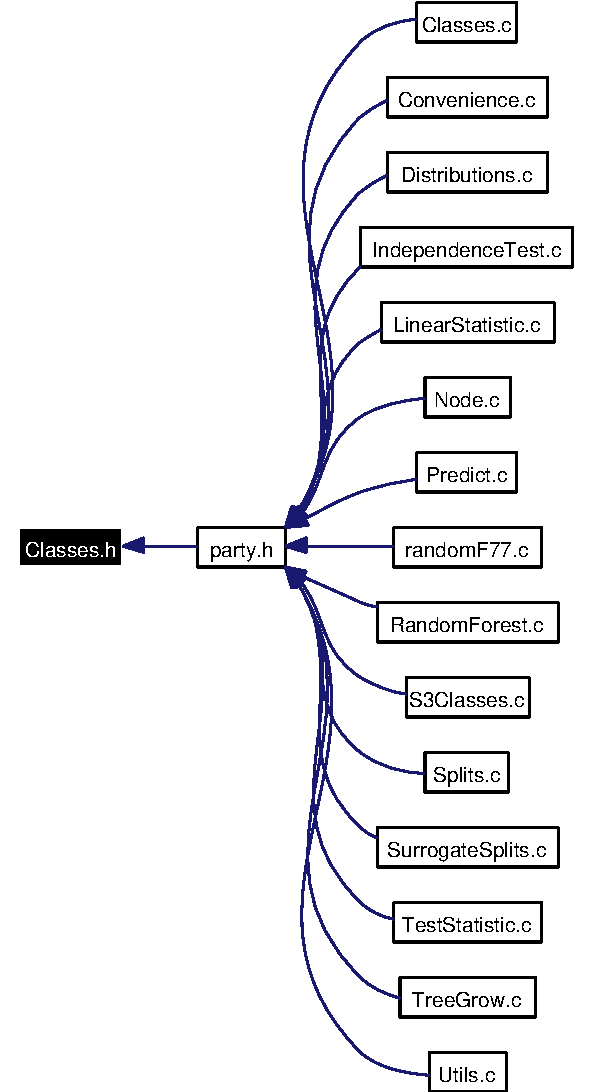
\includegraphics[width=163pt]{Classes_8h__dep__incl}
\end{center}
\end{figure}
\subsection*{Functions}
\begin{CompactItemize}
\item 
int \hyperlink{Classes_8h_8bc9164a2291bb7f61c12b79f6bc7c5f}{get\_\-dimension} (SEXP object)
\item 
int \hyperlink{Classes_8h_847e08eb9fce554539de3106ea03e9e2}{get\_\-teststat} (SEXP object)
\item 
double \hyperlink{Classes_8h_aa5df349ffd6e5faccab211ac972722b}{get\_\-tol} (SEXP object)
\item 
int \hyperlink{Classes_8h_309a9064403a71aba540cad646ba5854}{get\_\-pvalue} (SEXP object)
\item 
int \hyperlink{Classes_8h_b0fc0f7fb33f87cfa58cb8c617d946a1}{get\_\-maxpts} (SEXP object)
\item 
double \hyperlink{Classes_8h_4e2233c1c47758c555f99235f60984f0}{get\_\-abseps} (SEXP object)
\item 
double \hyperlink{Classes_8h_a17053ff24db1859af60e2d71baf924c}{get\_\-releps} (SEXP object)
\item 
double \hyperlink{Classes_8h_024b7f74a61afa9b3eb465a98f35584c}{get\_\-minsplit} (SEXP object)
\item 
double \hyperlink{Classes_8h_f7aaeccefe1bfbb1737ac3403a85c8e9}{get\_\-minprob} (SEXP object)
\item 
double \hyperlink{Classes_8h_0794d3cb26a60105140165d6dea3d70d}{get\_\-minbucket} (SEXP object)
\item 
SEXP \hyperlink{Classes_8h_20a55355301b5f90ec48b9114d1ff597}{get\_\-transformation} (SEXP object, int variable)
\item 
SEXP \hyperlink{Classes_8h_9ec50a13a7c7e82143cced16ff4f3968}{get\_\-test\_\-trafo} (SEXP object)
\item 
SEXP \hyperlink{Classes_8h_b86d70ff194260cc9bd391d3ff55b157}{get\_\-predict\_\-trafo} (SEXP object)
\item 
SEXP \hyperlink{Classes_8h_0f91efa916e815ec7d90c6f9516f18e4}{get\_\-variable} (SEXP object, int variable)
\item 
int \hyperlink{Classes_8h_f836613ade2cdc01c401b574fc1e7fdb}{is\_\-nominal} (SEXP object, int variable)
\item 
int \hyperlink{Classes_8h_53608524b90af1655d49496ec5ccbd47}{is\_\-ordinal} (SEXP object, int variable)
\item 
int \hyperlink{Classes_8h_2ea962f10f7adde8ad25429e15cad9d3}{is\_\-censored} (SEXP object, int variable)
\item 
int \hyperlink{Classes_8h_50548fbe6024d9a7118db3fce5085fd9}{has\_\-missings} (SEXP object, int variable)
\item 
SEXP \hyperlink{Classes_8h_fd6cfc2dd239b138d91e92a8ce9353f8}{get\_\-missings} (SEXP object, int variable)
\item 
SEXP \hyperlink{Classes_8h_a160107e2d687d3fa2411af7e25763ef}{get\_\-ordering} (SEXP object, int variable)
\item 
SEXP \hyperlink{Classes_8h_0e317821da8f3bc0fb6da5006abb81f6}{get\_\-levels} (SEXP object, int variable)
\item 
SEXP \hyperlink{Classes_8h_ba4726f56726372030e1e104b2f2b076}{get\_\-scores} (SEXP object, int variable)
\item 
SEXP \hyperlink{Classes_8h_e3c823841d28ac07932df6cf545563c5}{get\_\-which\-NA} (SEXP object, int variable)
\item 
SEXP \hyperlink{Classes_8h_31bf6c4f0764bc42b413cc319a0f9ec2}{get\_\-varmemory} (SEXP object, int variable)
\item 
int \hyperlink{Classes_8h_45df17685bc6c95d03fb65b6f6214de0}{get\_\-nobs} (SEXP object)
\item 
int \hyperlink{Classes_8h_9117d8f57ea1378c725c7299d6cc2923}{get\_\-ninputs} (SEXP object)
\item 
SEXP \hyperlink{Classes_8h_7088b22be6072c314107cab4e2bf7d2e}{get\_\-weights} (SEXP object, int variable)
\item 
int \hyperlink{Classes_8h_7f1c5e96481b726312de51ca7c6ef924}{get\_\-testtype} (SEXP object)
\item 
int \hyperlink{Classes_8h_af696af616c142e55ea0758690d20d7c}{get\_\-nresample} (SEXP object)
\item 
SEXP \hyperlink{Classes_8h_a7f64a77df0cfbcae9428aa6684a1ad1}{get\_\-varctrl} (SEXP object)
\item 
SEXP \hyperlink{Classes_8h_d914bd038dca4d2a1b9847f46bdb78f9}{get\_\-splitctrl} (SEXP object)
\item 
SEXP \hyperlink{Classes_8h_43fe1d056590d0d70d3a72beda13963e}{get\_\-gtctrl} (SEXP object)
\item 
double \hyperlink{Classes_8h_3578ef4fb8f0c3ecd7d166687acde94a}{get\_\-mincriterion} (SEXP object)
\item 
int \hyperlink{Classes_8h_79a38a57d0a4fbf5d7df55bf9a1dc66d}{get\_\-randomsplits} (SEXP object)
\item 
int \hyperlink{Classes_8h_5d34a7ec21d7c132111e87c1895e90fd}{get\_\-mtry} (SEXP object)
\item 
SEXP \hyperlink{Classes_8h_3598986a5115e969e9d435c5036dcecf}{get\_\-dontuse} (SEXP object)
\item 
SEXP \hyperlink{Classes_8h_3c02aa6a5a00bc0ca460e78540fa064c}{get\_\-dontusetmp} (SEXP object)
\item 
int \hyperlink{Classes_8h_c7779f00dc36c589dd24e3b4f6247be3}{get\_\-stump} (SEXP object)
\item 
int \hyperlink{Classes_8h_b89e4da7a60580c3adbe7c4f4935581c}{get\_\-maxsurrogate} (SEXP object)
\item 
SEXP \hyperlink{Classes_8h_a88e9e2563188b5500b48a6efaee9734}{get\_\-tgctrl} (SEXP object)
\item 
SEXP \hyperlink{Classes_8h_3a0ec14f5047b8c9bf8d8e6ba3c6e306}{get\_\-splitstatistics} (SEXP object)
\item 
int \hyperlink{Classes_8h_2c17918334d53626178a38518f9f25ff}{get\_\-savesplitstats} (SEXP object)
\item 
int \hyperlink{Classes_8h_871d0c7dc9639a559b15a8790268063d}{check\_\-depth} (SEXP object, int depth)
\item 
int \hyperlink{Classes_8h_899349b79a444c39ff23856bd802e096}{get\_\-ntree} (SEXP object)
\item 
int \hyperlink{Classes_8h_2c31f2150a75ae67496074deeaea1f96}{get\_\-replace} (SEXP object)
\item 
double \hyperlink{Classes_8h_3367507eb875c7601cdb9d77f15b5871}{get\_\-fraction} (SEXP object)
\end{CompactItemize}
\subsection*{Variables}
\begin{CompactItemize}
\item 
SEXP \hyperlink{Classes_8h_f0a2dc8073174e68e71d4d19266bab22}{PL2\_\-expectation\-Sym}
\item 
SEXP \hyperlink{Classes_8h_e033132aed4900e99ec36faf7352ea34}{PL2\_\-covariance\-Sym}
\item 
SEXP \hyperlink{Classes_8h_e36e22e2f694307e4d5af6dade35abc6}{PL2\_\-linearstatistic\-Sym}
\item 
SEXP \hyperlink{Classes_8h_4d117ff485f06bee9902f99246ac9c04}{PL2\_\-expcovinf\-Sym}
\item 
SEXP \hyperlink{Classes_8h_1f0d5394a08065f5e1a54608dac5916d}{PL2\_\-expcovinfss\-Sym}
\item 
SEXP \hyperlink{Classes_8h_72d079f51635b70b0a19dfe3bc6716c8}{PL2\_\-sumweights\-Sym}
\item 
SEXP \hyperlink{Classes_8h_b993e9eabf03921afdda536cd0d03ef3}{PL2\_\-dimension\-Sym}
\item 
SEXP \hyperlink{Classes_8h_6281f5e20196f03b8ca82137e9f0bee7}{PL2\_\-MPinv\-Sym}
\item 
SEXP \hyperlink{Classes_8h_2369f12a0df12fcae97775c41b461b63}{PL2\_\-rank\-Sym}
\item 
SEXP \hyperlink{Classes_8h_db458a813e63087567adf5522b10e5b3}{PL2\_\-svd\-Sym}
\item 
SEXP \hyperlink{Classes_8h_191eafdb9f05be24507087e4a0cb656d}{PL2\_\-svdmem\-Sym}
\item 
SEXP \hyperlink{Classes_8h_f132d3e468f57f7d311f7d682e28d59d}{PL2\_\-method\-Sym}
\item 
SEXP \hyperlink{Classes_8h_e5f84a192b44654299d3b2c6f7febb0b}{PL2\_\-jobu\-Sym}
\item 
SEXP \hyperlink{Classes_8h_faaa2e8cc7b0f2244d84dcd517ba3bf6}{PL2\_\-jobv\-Sym}
\item 
SEXP \hyperlink{Classes_8h_d81981007d31ea647673010bdd41bcc2}{PL2\_\-u\-Sym}
\item 
SEXP \hyperlink{Classes_8h_7362d58f9bd0581cf6c7b584d2783167}{PL2\_\-v\-Sym}
\item 
SEXP \hyperlink{Classes_8h_d9bc9a01dae6a98d2709e4d8b26124e8}{PL2\_\-s\-Sym}
\item 
SEXP \hyperlink{Classes_8h_d088d7d8474d9c927044da9ba5f37837}{PL2\_\-p\-Sym}
\item 
SEXP \hyperlink{Classes_8h_e430cc10639e774cf1b3daa8bbbe5496}{PL2\_\-teststat\-Sym}
\item 
SEXP \hyperlink{Classes_8h_969daa58978bef428c6c6938e5113509}{PL2\_\-pvalue\-Sym}
\item 
SEXP \hyperlink{Classes_8h_824c4bd02d12a3dd1d316a51fe622b0c}{PL2\_\-tol\-Sym}
\item 
SEXP \hyperlink{Classes_8h_87248987fad9ad3b05be6d24eba22886}{PL2\_\-maxpts\-Sym}
\item 
SEXP \hyperlink{Classes_8h_c4c2f757e83d183b6a85addfb8713c4c}{PL2\_\-abseps\-Sym}
\item 
SEXP \hyperlink{Classes_8h_1b283af10ddc0589b96baa42d609f237}{PL2\_\-releps\-Sym}
\item 
SEXP \hyperlink{Classes_8h_109785d63340f9ae8e21f0b6dde2aa20}{PL2\_\-minsplit\-Sym}
\item 
SEXP \hyperlink{Classes_8h_c973393fe44233f4b23dc2f11a30f908}{PL2\_\-minbucket\-Sym}
\item 
SEXP \hyperlink{Classes_8h_956e5ea52c0c35b429e14619e7f94ee5}{PL2\_\-minprob\-Sym}
\item 
SEXP \hyperlink{Classes_8h_94e141e6d1a1315e28d142860b5f987e}{PL2\_\-variables\-Sym}
\item 
SEXP \hyperlink{Classes_8h_6f387307dcb17869091e08e6c7d5a5c5}{PL2\_\-transformations\-Sym}
\item 
SEXP \hyperlink{Classes_8h_7fc0ba403124f5d582b0e5abd13f4fb4}{PL2\_\-is\_\-nominal\-Sym}
\item 
SEXP \hyperlink{Classes_8h_619562059f34e6d80cac945f03efd16c}{PL2\_\-is\_\-ordinal\-Sym}
\item 
SEXP \hyperlink{Classes_8h_b599a0472b4568fbc3111f315ebb035f}{PL2\_\-is\_\-censored\-Sym}
\item 
SEXP \hyperlink{Classes_8h_6a6f78bf6df3ce35b0d6315db7e60165}{PL2\_\-ordering\-Sym}
\item 
SEXP \hyperlink{Classes_8h_780ff4fae7d4b234b757caf5cec27a35}{PL2\_\-levels\-Sym}
\item 
SEXP \hyperlink{Classes_8h_68c23c34260e4a4863e5c0caf2b3b411}{PL2\_\-scores\-Sym}
\item 
SEXP \hyperlink{Classes_8h_6cad742d32f0ac66eb12db5312c062b6}{PL2\_\-has\_\-missings\-Sym}
\item 
SEXP \hyperlink{Classes_8h_48fecaa469261c6beb2abb11970a29ef}{PL2\_\-which\-NASym}
\item 
SEXP \hyperlink{Classes_8h_16a47750f3b0a7e3261132bc24c1cdde}{PL2\_\-test\_\-trafo\-Sym}
\item 
SEXP \hyperlink{Classes_8h_727b86d73186990d5620eb01e39b2707}{PL2\_\-predict\_\-trafo\-Sym}
\item 
SEXP \hyperlink{Classes_8h_eb411e47896a840cc77dd3cae74533d8}{PL2\_\-nobs\-Sym}
\item 
SEXP \hyperlink{Classes_8h_4cc863cbaafba964bbc10a4ad7b90c72}{PL2\_\-ninputs\-Sym}
\item 
SEXP \hyperlink{Classes_8h_adb3a293553f93d6233d9ba4ab7d1039}{PL2\_\-linexpcov2sample\-Sym}
\item 
SEXP \hyperlink{Classes_8h_81fa0afba4ad786166ef0872c842a9db}{PL2\_\-weights\-Sym}
\item 
SEXP \hyperlink{Classes_8h_6b4204d372191db8c7fb0210bfce8f6a}{PL2\_\-varmemory\-Sym}
\item 
SEXP \hyperlink{Classes_8h_adb3a293553f93d6233d9ba4ab7d1039}{PL2\_\-linexpcov2sample\-Sym}
\item 
SEXP \hyperlink{Classes_8h_81fa0afba4ad786166ef0872c842a9db}{PL2\_\-weights\-Sym}
\item 
SEXP \hyperlink{Classes_8h_6b4204d372191db8c7fb0210bfce8f6a}{PL2\_\-varmemory\-Sym}
\item 
SEXP \hyperlink{Classes_8h_9ad5f5cd65458d95a8ffae2d450ec850}{PL2\_\-responses\-Sym}
\item 
SEXP \hyperlink{Classes_8h_a0f1db0215808916904d250b11f71edd}{PL2\_\-inputs\-Sym}
\item 
SEXP \hyperlink{Classes_8h_81b84b3f654314ad4bd6885dad350ad3}{PL2\_\-testtype\-Sym}
\item 
SEXP \hyperlink{Classes_8h_0ca6293b541d65ee9205ef090e3a89c0}{PL2\_\-nresample\-Sym}
\item 
SEXP \hyperlink{Classes_8h_590494b5bcca46b1624c9cfb40e3fa7a}{PL2\_\-varctrl\-Sym}
\item 
SEXP \hyperlink{Classes_8h_a416b1a8d0e742414f07cecc14b2ff22}{PL2\_\-splitctrl\-Sym}
\item 
SEXP \hyperlink{Classes_8h_3624cf464666d668ac01bd82e1dbb67e}{PL2\_\-gtctrl\-Sym}
\item 
SEXP \hyperlink{Classes_8h_4978acb0c711be68d72823f0e4b6141e}{PL2\_\-mincriterion\-Sym}
\item 
SEXP \hyperlink{Classes_8h_773e1edf30b724c5335c1276ed3c6a6c}{PL2\_\-randomsplits\-Sym}
\item 
SEXP \hyperlink{Classes_8h_59e6ce8e5bed48dcf9299d9a7bff933d}{PL2\_\-mtry\-Sym}
\item 
SEXP \hyperlink{Classes_8h_38ddf1da2b9d162d074d1f5c6d5c0418}{PL2\_\-dontuse\-Sym}
\item 
SEXP \hyperlink{Classes_8h_60440f0803a2789589834032edcc31f5}{PL2\_\-dontusetmp\-Sym}
\item 
SEXP \hyperlink{Classes_8h_ba1a6d09a1f030c9dea1b11dc46e2f1a}{PL2\_\-stump\-Sym}
\item 
SEXP \hyperlink{Classes_8h_9b2381d5cefcc57f5fa2e140167ecb9d}{PL2\_\-tgctrl\-Sym}
\item 
SEXP \hyperlink{Classes_8h_8c22189efef525e27fd3793ca37aa109}{PL2\_\-ntree\-Sym}
\item 
SEXP \hyperlink{Classes_8h_4b88d1bbcab84cb3e7d1e634d9df1af2}{PL2\_\-replace\-Sym}
\item 
SEXP \hyperlink{Classes_8h_3beca0734adb10de599aa3c2e2d9f329}{PL2\_\-fraction\-Sym}
\end{CompactItemize}


\subsection{Function Documentation}
\hypertarget{Classes_8h_871d0c7dc9639a559b15a8790268063d}{
\index{Classes.h@{Classes.h}!check_depth@{check\_\-depth}}
\index{check_depth@{check\_\-depth}!Classes.h@{Classes.h}}
\subsubsection[check\_\-depth]{\setlength{\rightskip}{0pt plus 5cm}int check\_\-depth (SEXP {\em object}, int {\em depth})}}
\label{Classes_8h_871d0c7dc9639a559b15a8790268063d}




Definition at line 348 of file Classes.c.

References PL2\_\-maxdepth\-Sym.

Referenced by C\_\-Tree\-Grow().\hypertarget{Classes_8h_4e2233c1c47758c555f99235f60984f0}{
\index{Classes.h@{Classes.h}!get_abseps@{get\_\-abseps}}
\index{get_abseps@{get\_\-abseps}!Classes.h@{Classes.h}}
\subsubsection[get\_\-abseps]{\setlength{\rightskip}{0pt plus 5cm}double get\_\-abseps (SEXP {\em object})}}
\label{Classes_8h_4e2233c1c47758c555f99235f60984f0}




Definition at line 169 of file Classes.c.

References PL2\_\-abseps\-Sym.

Referenced by C\_\-Teststat\-Pvalue().\hypertarget{Classes_8h_8bc9164a2291bb7f61c12b79f6bc7c5f}{
\index{Classes.h@{Classes.h}!get_dimension@{get\_\-dimension}}
\index{get_dimension@{get\_\-dimension}!Classes.h@{Classes.h}}
\subsubsection[get\_\-dimension]{\setlength{\rightskip}{0pt plus 5cm}int get\_\-dimension (SEXP {\em object})}}
\label{Classes_8h_8bc9164a2291bb7f61c12b79f6bc7c5f}




Definition at line 149 of file Classes.c.

References PL2\_\-dimension\-Sym.

Referenced by C\_\-Conditional\-Pvalue(), C\_\-Node(), C\_\-Test\-Statistic(), and R\_\-splitcategorical().\hypertarget{Classes_8h_3598986a5115e969e9d435c5036dcecf}{
\index{Classes.h@{Classes.h}!get_dontuse@{get\_\-dontuse}}
\index{get_dontuse@{get\_\-dontuse}!Classes.h@{Classes.h}}
\subsubsection[get\_\-dontuse]{\setlength{\rightskip}{0pt plus 5cm}SEXP get\_\-dontuse (SEXP {\em object})}}
\label{Classes_8h_3598986a5115e969e9d435c5036dcecf}




Definition at line 336 of file Classes.c.

References PL2\_\-dontuse\-Sym.\hypertarget{Classes_8h_3c02aa6a5a00bc0ca460e78540fa064c}{
\index{Classes.h@{Classes.h}!get_dontusetmp@{get\_\-dontusetmp}}
\index{get_dontusetmp@{get\_\-dontusetmp}!Classes.h@{Classes.h}}
\subsubsection[get\_\-dontusetmp]{\setlength{\rightskip}{0pt plus 5cm}SEXP get\_\-dontusetmp (SEXP {\em object})}}
\label{Classes_8h_3c02aa6a5a00bc0ca460e78540fa064c}




Definition at line 340 of file Classes.c.

References PL2\_\-dontusetmp\-Sym.\hypertarget{Classes_8h_3367507eb875c7601cdb9d77f15b5871}{
\index{Classes.h@{Classes.h}!get_fraction@{get\_\-fraction}}
\index{get_fraction@{get\_\-fraction}!Classes.h@{Classes.h}}
\subsubsection[get\_\-fraction]{\setlength{\rightskip}{0pt plus 5cm}double get\_\-fraction (SEXP {\em object})}}
\label{Classes_8h_3367507eb875c7601cdb9d77f15b5871}




Definition at line 364 of file Classes.c.

References PL2\_\-fraction\-Sym.\hypertarget{Classes_8h_43fe1d056590d0d70d3a72beda13963e}{
\index{Classes.h@{Classes.h}!get_gtctrl@{get\_\-gtctrl}}
\index{get_gtctrl@{get\_\-gtctrl}!Classes.h@{Classes.h}}
\subsubsection[get\_\-gtctrl]{\setlength{\rightskip}{0pt plus 5cm}SEXP get\_\-gtctrl (SEXP {\em object})}}
\label{Classes_8h_43fe1d056590d0d70d3a72beda13963e}




Definition at line 312 of file Classes.c.

References PL2\_\-gtctrl\-Sym.

Referenced by C\_\-Node().\hypertarget{Classes_8h_0e317821da8f3bc0fb6da5006abb81f6}{
\index{Classes.h@{Classes.h}!get_levels@{get\_\-levels}}
\index{get_levels@{get\_\-levels}!Classes.h@{Classes.h}}
\subsubsection[get\_\-levels]{\setlength{\rightskip}{0pt plus 5cm}SEXP get\_\-levels (SEXP {\em object}, int {\em variable})}}
\label{Classes_8h_0e317821da8f3bc0fb6da5006abb81f6}




Definition at line 237 of file Classes.c.

References is\_\-nominal(), is\_\-ordinal(), and PL2\_\-levels\-Sym.

Referenced by C\_\-Node().

Here is the call graph for this function:\begin{figure}[H]
\begin{center}
\leavevmode
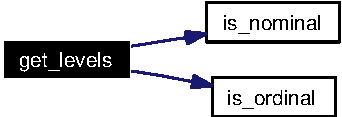
\includegraphics[width=99pt]{Classes_8h_0e317821da8f3bc0fb6da5006abb81f6_cgraph}
\end{center}
\end{figure}
\hypertarget{Classes_8h_b0fc0f7fb33f87cfa58cb8c617d946a1}{
\index{Classes.h@{Classes.h}!get_maxpts@{get\_\-maxpts}}
\index{get_maxpts@{get\_\-maxpts}!Classes.h@{Classes.h}}
\subsubsection[get\_\-maxpts]{\setlength{\rightskip}{0pt plus 5cm}int get\_\-maxpts (SEXP {\em object})}}
\label{Classes_8h_b0fc0f7fb33f87cfa58cb8c617d946a1}




Definition at line 165 of file Classes.c.

References PL2\_\-maxpts\-Sym.

Referenced by C\_\-Teststat\-Pvalue().\hypertarget{Classes_8h_b89e4da7a60580c3adbe7c4f4935581c}{
\index{Classes.h@{Classes.h}!get_maxsurrogate@{get\_\-maxsurrogate}}
\index{get_maxsurrogate@{get\_\-maxsurrogate}!Classes.h@{Classes.h}}
\subsubsection[get\_\-maxsurrogate]{\setlength{\rightskip}{0pt plus 5cm}int get\_\-maxsurrogate (SEXP {\em object})}}
\label{Classes_8h_b89e4da7a60580c3adbe7c4f4935581c}




Definition at line 324 of file Classes.c.

References PL2\_\-maxsurrogate\-Sym.

Referenced by C\_\-splitnode(), C\_\-surrogates(), C\_\-Tree\-Grow(), R\_\-Node(), and R\_\-Tree\-Grow().\hypertarget{Classes_8h_0794d3cb26a60105140165d6dea3d70d}{
\index{Classes.h@{Classes.h}!get_minbucket@{get\_\-minbucket}}
\index{get_minbucket@{get\_\-minbucket}!Classes.h@{Classes.h}}
\subsubsection[get\_\-minbucket]{\setlength{\rightskip}{0pt plus 5cm}double get\_\-minbucket (SEXP {\em object})}}
\label{Classes_8h_0794d3cb26a60105140165d6dea3d70d}




Definition at line 185 of file Classes.c.

References PL2\_\-minbucket\-Sym.\hypertarget{Classes_8h_3578ef4fb8f0c3ecd7d166687acde94a}{
\index{Classes.h@{Classes.h}!get_mincriterion@{get\_\-mincriterion}}
\index{get_mincriterion@{get\_\-mincriterion}!Classes.h@{Classes.h}}
\subsubsection[get\_\-mincriterion]{\setlength{\rightskip}{0pt plus 5cm}double get\_\-mincriterion (SEXP {\em object})}}
\label{Classes_8h_3578ef4fb8f0c3ecd7d166687acde94a}




Definition at line 320 of file Classes.c.

References PL2\_\-mincriterion\-Sym.

Referenced by C\_\-Node().\hypertarget{Classes_8h_f7aaeccefe1bfbb1737ac3403a85c8e9}{
\index{Classes.h@{Classes.h}!get_minprob@{get\_\-minprob}}
\index{get_minprob@{get\_\-minprob}!Classes.h@{Classes.h}}
\subsubsection[get\_\-minprob]{\setlength{\rightskip}{0pt plus 5cm}double get\_\-minprob (SEXP {\em object})}}
\label{Classes_8h_f7aaeccefe1bfbb1737ac3403a85c8e9}




Definition at line 181 of file Classes.c.

References PL2\_\-minprob\-Sym.\hypertarget{Classes_8h_024b7f74a61afa9b3eb465a98f35584c}{
\index{Classes.h@{Classes.h}!get_minsplit@{get\_\-minsplit}}
\index{get_minsplit@{get\_\-minsplit}!Classes.h@{Classes.h}}
\subsubsection[get\_\-minsplit]{\setlength{\rightskip}{0pt plus 5cm}double get\_\-minsplit (SEXP {\em object})}}
\label{Classes_8h_024b7f74a61afa9b3eb465a98f35584c}




Definition at line 177 of file Classes.c.

References PL2\_\-minsplit\-Sym.

Referenced by C\_\-Node().\hypertarget{Classes_8h_fd6cfc2dd239b138d91e92a8ce9353f8}{
\index{Classes.h@{Classes.h}!get_missings@{get\_\-missings}}
\index{get_missings@{get\_\-missings}!Classes.h@{Classes.h}}
\subsubsection[get\_\-missings]{\setlength{\rightskip}{0pt plus 5cm}SEXP get\_\-missings (SEXP {\em object}, int {\em variable})}}
\label{Classes_8h_fd6cfc2dd239b138d91e92a8ce9353f8}




Definition at line 260 of file Classes.c.

References has\_\-missings(), and PL2\_\-which\-NASym.

Referenced by C\_\-get\_\-node(), C\_\-splitnode(), C\_\-splitsurrogate(), and C\_\-surrogates().

Here is the call graph for this function:\begin{figure}[H]
\begin{center}
\leavevmode
\includegraphics[width=113pt]{Classes_8h_fd6cfc2dd239b138d91e92a8ce9353f8_cgraph}
\end{center}
\end{figure}
\hypertarget{Classes_8h_5d34a7ec21d7c132111e87c1895e90fd}{
\index{Classes.h@{Classes.h}!get_mtry@{get\_\-mtry}}
\index{get_mtry@{get\_\-mtry}!Classes.h@{Classes.h}}
\subsubsection[get\_\-mtry]{\setlength{\rightskip}{0pt plus 5cm}int get\_\-mtry (SEXP {\em object})}}
\label{Classes_8h_5d34a7ec21d7c132111e87c1895e90fd}




Definition at line 332 of file Classes.c.

References PL2\_\-mtry\-Sym.\hypertarget{Classes_8h_9117d8f57ea1378c725c7299d6cc2923}{
\index{Classes.h@{Classes.h}!get_ninputs@{get\_\-ninputs}}
\index{get_ninputs@{get\_\-ninputs}!Classes.h@{Classes.h}}
\subsubsection[get\_\-ninputs]{\setlength{\rightskip}{0pt plus 5cm}int get\_\-ninputs (SEXP {\em object})}}
\label{Classes_8h_9117d8f57ea1378c725c7299d6cc2923}




Definition at line 288 of file Classes.c.

References PL2\_\-ninputs\-Sym.

Referenced by C\_\-Global\-Test(), C\_\-Monte\-Carlo(), C\_\-Node(), C\_\-splitnode(), C\_\-surrogates(), R\_\-Global\-Test(), R\_\-Monte\-Carlo(), R\_\-Node(), and R\_\-Tree\-Grow().\hypertarget{Classes_8h_45df17685bc6c95d03fb65b6f6214de0}{
\index{Classes.h@{Classes.h}!get_nobs@{get\_\-nobs}}
\index{get_nobs@{get\_\-nobs}!Classes.h@{Classes.h}}
\subsubsection[get\_\-nobs]{\setlength{\rightskip}{0pt plus 5cm}int get\_\-nobs (SEXP {\em object})}}
\label{Classes_8h_45df17685bc6c95d03fb65b6f6214de0}




Definition at line 284 of file Classes.c.

References PL2\_\-nobs\-Sym.

Referenced by C\_\-Global\-Test(), C\_\-Monte\-Carlo(), C\_\-Node(), C\_\-predict(), C\_\-splitnode(), C\_\-splitsurrogate(), C\_\-surrogates(), C\_\-Tree\-Grow(), C\_\-weights(), R\_\-Ensemble(), R\_\-get\_\-node\-ID(), R\_\-Node(), R\_\-predict(), R\_\-predict\-RF(), R\_\-predict\-RF2(), R\_\-predict\-RF\_\-weights(), R\_\-Tree\-Grow(), and R\_\-weights().\hypertarget{Classes_8h_af696af616c142e55ea0758690d20d7c}{
\index{Classes.h@{Classes.h}!get_nresample@{get\_\-nresample}}
\index{get_nresample@{get\_\-nresample}!Classes.h@{Classes.h}}
\subsubsection[get\_\-nresample]{\setlength{\rightskip}{0pt plus 5cm}int get\_\-nresample (SEXP {\em object})}}
\label{Classes_8h_af696af616c142e55ea0758690d20d7c}




Definition at line 300 of file Classes.c.

References PL2\_\-nresample\-Sym.

Referenced by C\_\-Monte\-Carlo().\hypertarget{Classes_8h_899349b79a444c39ff23856bd802e096}{
\index{Classes.h@{Classes.h}!get_ntree@{get\_\-ntree}}
\index{get_ntree@{get\_\-ntree}!Classes.h@{Classes.h}}
\subsubsection[get\_\-ntree]{\setlength{\rightskip}{0pt plus 5cm}int get\_\-ntree (SEXP {\em object})}}
\label{Classes_8h_899349b79a444c39ff23856bd802e096}




Definition at line 356 of file Classes.c.

References PL2\_\-ntree\-Sym.

Referenced by R\_\-Ensemble().\hypertarget{Classes_8h_a160107e2d687d3fa2411af7e25763ef}{
\index{Classes.h@{Classes.h}!get_ordering@{get\_\-ordering}}
\index{get_ordering@{get\_\-ordering}!Classes.h@{Classes.h}}
\subsubsection[get\_\-ordering]{\setlength{\rightskip}{0pt plus 5cm}SEXP get\_\-ordering (SEXP {\em object}, int {\em variable})}}
\label{Classes_8h_a160107e2d687d3fa2411af7e25763ef}




Definition at line 226 of file Classes.c.

References is\_\-nominal(), and PL2\_\-ordering\-Sym.

Referenced by C\_\-Node().

Here is the call graph for this function:\begin{figure}[H]
\begin{center}
\leavevmode
\includegraphics[width=105pt]{Classes_8h_a160107e2d687d3fa2411af7e25763ef_cgraph}
\end{center}
\end{figure}
\hypertarget{Classes_8h_b86d70ff194260cc9bd391d3ff55b157}{
\index{Classes.h@{Classes.h}!get_predict_trafo@{get\_\-predict\_\-trafo}}
\index{get_predict_trafo@{get\_\-predict\_\-trafo}!Classes.h@{Classes.h}}
\subsubsection[get\_\-predict\_\-trafo]{\setlength{\rightskip}{0pt plus 5cm}SEXP get\_\-predict\_\-trafo (SEXP {\em object})}}
\label{Classes_8h_b86d70ff194260cc9bd391d3ff55b157}




Definition at line 199 of file Classes.c.

References PL2\_\-predict\_\-trafo\-Sym.

Referenced by C\_\-Node(), C\_\-splitnode(), R\_\-modify\_\-response(), R\_\-Node(), R\_\-set\_\-response(), and R\_\-Tree\-Grow().\hypertarget{Classes_8h_309a9064403a71aba540cad646ba5854}{
\index{Classes.h@{Classes.h}!get_pvalue@{get\_\-pvalue}}
\index{get_pvalue@{get\_\-pvalue}!Classes.h@{Classes.h}}
\subsubsection[get\_\-pvalue]{\setlength{\rightskip}{0pt plus 5cm}int get\_\-pvalue (SEXP {\em object})}}
\label{Classes_8h_309a9064403a71aba540cad646ba5854}




Definition at line 157 of file Classes.c.

References PL2\_\-pvalue\-Sym.

Referenced by C\_\-Teststat\-Criterion(), and C\_\-Teststat\-Pvalue().\hypertarget{Classes_8h_79a38a57d0a4fbf5d7df55bf9a1dc66d}{
\index{Classes.h@{Classes.h}!get_randomsplits@{get\_\-randomsplits}}
\index{get_randomsplits@{get\_\-randomsplits}!Classes.h@{Classes.h}}
\subsubsection[get\_\-randomsplits]{\setlength{\rightskip}{0pt plus 5cm}int get\_\-randomsplits (SEXP {\em object})}}
\label{Classes_8h_79a38a57d0a4fbf5d7df55bf9a1dc66d}




Definition at line 328 of file Classes.c.

References PL2\_\-randomsplits\-Sym.\hypertarget{Classes_8h_a17053ff24db1859af60e2d71baf924c}{
\index{Classes.h@{Classes.h}!get_releps@{get\_\-releps}}
\index{get_releps@{get\_\-releps}!Classes.h@{Classes.h}}
\subsubsection[get\_\-releps]{\setlength{\rightskip}{0pt plus 5cm}double get\_\-releps (SEXP {\em object})}}
\label{Classes_8h_a17053ff24db1859af60e2d71baf924c}




Definition at line 173 of file Classes.c.

References PL2\_\-releps\-Sym.

Referenced by C\_\-Teststat\-Pvalue().\hypertarget{Classes_8h_2c31f2150a75ae67496074deeaea1f96}{
\index{Classes.h@{Classes.h}!get_replace@{get\_\-replace}}
\index{get_replace@{get\_\-replace}!Classes.h@{Classes.h}}
\subsubsection[get\_\-replace]{\setlength{\rightskip}{0pt plus 5cm}int get\_\-replace (SEXP {\em object})}}
\label{Classes_8h_2c31f2150a75ae67496074deeaea1f96}




Definition at line 360 of file Classes.c.

References PL2\_\-replace\-Sym.\hypertarget{Classes_8h_2c17918334d53626178a38518f9f25ff}{
\index{Classes.h@{Classes.h}!get_savesplitstats@{get\_\-savesplitstats}}
\index{get_savesplitstats@{get\_\-savesplitstats}!Classes.h@{Classes.h}}
\subsubsection[get\_\-savesplitstats]{\setlength{\rightskip}{0pt plus 5cm}int get\_\-savesplitstats (SEXP {\em object})}}
\label{Classes_8h_2c17918334d53626178a38518f9f25ff}




Definition at line 276 of file Classes.c.

References PL2\_\-savesplitstats\-Sym.

Referenced by C\_\-Node().\hypertarget{Classes_8h_ba4726f56726372030e1e104b2f2b076}{
\index{Classes.h@{Classes.h}!get_scores@{get\_\-scores}}
\index{get_scores@{get\_\-scores}!Classes.h@{Classes.h}}
\subsubsection[get\_\-scores]{\setlength{\rightskip}{0pt plus 5cm}SEXP get\_\-scores (SEXP {\em object}, int {\em variable})}}
\label{Classes_8h_ba4726f56726372030e1e104b2f2b076}




Definition at line 249 of file Classes.c.

References is\_\-ordinal(), and PL2\_\-scores\-Sym.

Here is the call graph for this function:\begin{figure}[H]
\begin{center}
\leavevmode
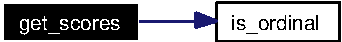
\includegraphics[width=99pt]{Classes_8h_ba4726f56726372030e1e104b2f2b076_cgraph}
\end{center}
\end{figure}
\hypertarget{Classes_8h_d914bd038dca4d2a1b9847f46bdb78f9}{
\index{Classes.h@{Classes.h}!get_splitctrl@{get\_\-splitctrl}}
\index{get_splitctrl@{get\_\-splitctrl}!Classes.h@{Classes.h}}
\subsubsection[get\_\-splitctrl]{\setlength{\rightskip}{0pt plus 5cm}SEXP get\_\-splitctrl (SEXP {\em object})}}
\label{Classes_8h_d914bd038dca4d2a1b9847f46bdb78f9}




Definition at line 308 of file Classes.c.

References PL2\_\-splitctrl\-Sym.

Referenced by C\_\-Node(), C\_\-splitnode(), C\_\-surrogates(), C\_\-Tree\-Grow(), R\_\-Node(), and R\_\-Tree\-Grow().\hypertarget{Classes_8h_3a0ec14f5047b8c9bf8d8e6ba3c6e306}{
\index{Classes.h@{Classes.h}!get_splitstatistics@{get\_\-splitstatistics}}
\index{get_splitstatistics@{get\_\-splitstatistics}!Classes.h@{Classes.h}}
\subsubsection[get\_\-splitstatistics]{\setlength{\rightskip}{0pt plus 5cm}SEXP get\_\-splitstatistics (SEXP {\em object})}}
\label{Classes_8h_3a0ec14f5047b8c9bf8d8e6ba3c6e306}




Definition at line 280 of file Classes.c.

References PL2\_\-splitstatistics\-Sym.

Referenced by C\_\-Node().\hypertarget{Classes_8h_c7779f00dc36c589dd24e3b4f6247be3}{
\index{Classes.h@{Classes.h}!get_stump@{get\_\-stump}}
\index{get_stump@{get\_\-stump}!Classes.h@{Classes.h}}
\subsubsection[get\_\-stump]{\setlength{\rightskip}{0pt plus 5cm}int get\_\-stump (SEXP {\em object})}}
\label{Classes_8h_c7779f00dc36c589dd24e3b4f6247be3}




Definition at line 344 of file Classes.c.

References PL2\_\-stump\-Sym.

Referenced by C\_\-Tree\-Grow().\hypertarget{Classes_8h_9ec50a13a7c7e82143cced16ff4f3968}{
\index{Classes.h@{Classes.h}!get_test_trafo@{get\_\-test\_\-trafo}}
\index{get_test_trafo@{get\_\-test\_\-trafo}!Classes.h@{Classes.h}}
\subsubsection[get\_\-test\_\-trafo]{\setlength{\rightskip}{0pt plus 5cm}SEXP get\_\-test\_\-trafo (SEXP {\em object})}}
\label{Classes_8h_9ec50a13a7c7e82143cced16ff4f3968}




Definition at line 195 of file Classes.c.

References PL2\_\-test\_\-trafo\-Sym.

Referenced by C\_\-Global\-Test(), C\_\-Monte\-Carlo(), C\_\-Node(), R\_\-modify\_\-response(), and R\_\-set\_\-response().\hypertarget{Classes_8h_847e08eb9fce554539de3106ea03e9e2}{
\index{Classes.h@{Classes.h}!get_teststat@{get\_\-teststat}}
\index{get_teststat@{get\_\-teststat}!Classes.h@{Classes.h}}
\subsubsection[get\_\-teststat]{\setlength{\rightskip}{0pt plus 5cm}int get\_\-teststat (SEXP {\em object})}}
\label{Classes_8h_847e08eb9fce554539de3106ea03e9e2}




Definition at line 153 of file Classes.c.

References PL2\_\-teststat\-Sym.

Referenced by C\_\-Independence\-Test(), and C\_\-Teststat\-Pvalue().\hypertarget{Classes_8h_7f1c5e96481b726312de51ca7c6ef924}{
\index{Classes.h@{Classes.h}!get_testtype@{get\_\-testtype}}
\index{get_testtype@{get\_\-testtype}!Classes.h@{Classes.h}}
\subsubsection[get\_\-testtype]{\setlength{\rightskip}{0pt plus 5cm}int get\_\-testtype (SEXP {\em object})}}
\label{Classes_8h_7f1c5e96481b726312de51ca7c6ef924}




Definition at line 296 of file Classes.c.

References PL2\_\-testtype\-Sym.\hypertarget{Classes_8h_a88e9e2563188b5500b48a6efaee9734}{
\index{Classes.h@{Classes.h}!get_tgctrl@{get\_\-tgctrl}}
\index{get_tgctrl@{get\_\-tgctrl}!Classes.h@{Classes.h}}
\subsubsection[get\_\-tgctrl]{\setlength{\rightskip}{0pt plus 5cm}SEXP get\_\-tgctrl (SEXP {\em object})}}
\label{Classes_8h_a88e9e2563188b5500b48a6efaee9734}




Definition at line 316 of file Classes.c.

References PL2\_\-tgctrl\-Sym.

Referenced by C\_\-Node(), and C\_\-Tree\-Grow().\hypertarget{Classes_8h_aa5df349ffd6e5faccab211ac972722b}{
\index{Classes.h@{Classes.h}!get_tol@{get\_\-tol}}
\index{get_tol@{get\_\-tol}!Classes.h@{Classes.h}}
\subsubsection[get\_\-tol]{\setlength{\rightskip}{0pt plus 5cm}double get\_\-tol (SEXP {\em object})}}
\label{Classes_8h_aa5df349ffd6e5faccab211ac972722b}




Definition at line 161 of file Classes.c.

References PL2\_\-tol\-Sym.

Referenced by C\_\-Independence\-Test(), C\_\-Node(), C\_\-split(), C\_\-splitcategorical(), C\_\-Teststat\-Pvalue(), and R\_\-splitcategorical().\hypertarget{Classes_8h_20a55355301b5f90ec48b9114d1ff597}{
\index{Classes.h@{Classes.h}!get_transformation@{get\_\-transformation}}
\index{get_transformation@{get\_\-transformation}!Classes.h@{Classes.h}}
\subsubsection[get\_\-transformation]{\setlength{\rightskip}{0pt plus 5cm}SEXP get\_\-transformation (SEXP {\em object}, int {\em variable})}}
\label{Classes_8h_20a55355301b5f90ec48b9114d1ff597}




Definition at line 189 of file Classes.c.

References PL2\_\-transformations\-Sym.

Referenced by C\_\-Node(), and R\_\-modify\_\-response().\hypertarget{Classes_8h_a7f64a77df0cfbcae9428aa6684a1ad1}{
\index{Classes.h@{Classes.h}!get_varctrl@{get\_\-varctrl}}
\index{get_varctrl@{get\_\-varctrl}!Classes.h@{Classes.h}}
\subsubsection[get\_\-varctrl]{\setlength{\rightskip}{0pt plus 5cm}SEXP get\_\-varctrl (SEXP {\em object})}}
\label{Classes_8h_a7f64a77df0cfbcae9428aa6684a1ad1}




Definition at line 304 of file Classes.c.

References PL2\_\-varctrl\-Sym.

Referenced by C\_\-Node().\hypertarget{Classes_8h_0f91efa916e815ec7d90c6f9516f18e4}{
\index{Classes.h@{Classes.h}!get_variable@{get\_\-variable}}
\index{get_variable@{get\_\-variable}!Classes.h@{Classes.h}}
\subsubsection[get\_\-variable]{\setlength{\rightskip}{0pt plus 5cm}SEXP get\_\-variable (SEXP {\em object}, int {\em variable})}}
\label{Classes_8h_0f91efa916e815ec7d90c6f9516f18e4}




Definition at line 204 of file Classes.c.

References PL2\_\-variables\-Sym.

Referenced by C\_\-get\_\-node(), C\_\-Node(), C\_\-splitnode(), C\_\-splitsurrogate(), and R\_\-modify\_\-response().\hypertarget{Classes_8h_31bf6c4f0764bc42b413cc319a0f9ec2}{
\index{Classes.h@{Classes.h}!get_varmemory@{get\_\-varmemory}}
\index{get_varmemory@{get\_\-varmemory}!Classes.h@{Classes.h}}
\subsubsection[get\_\-varmemory]{\setlength{\rightskip}{0pt plus 5cm}SEXP get\_\-varmemory (SEXP {\em object}, int {\em variable})}}
\label{Classes_8h_31bf6c4f0764bc42b413cc319a0f9ec2}




Definition at line 271 of file Classes.c.

References PL2\_\-varmemory\-Sym.

Referenced by C\_\-Node().\hypertarget{Classes_8h_7088b22be6072c314107cab4e2bf7d2e}{
\index{Classes.h@{Classes.h}!get_weights@{get\_\-weights}}
\index{get_weights@{get\_\-weights}!Classes.h@{Classes.h}}
\subsubsection[get\_\-weights]{\setlength{\rightskip}{0pt plus 5cm}SEXP get\_\-weights (SEXP {\em object}, int {\em variable})}}
\label{Classes_8h_7088b22be6072c314107cab4e2bf7d2e}




Definition at line 292 of file Classes.c.

References PL2\_\-weights\-Sym.

Referenced by C\_\-Node().\hypertarget{Classes_8h_e3c823841d28ac07932df6cf545563c5}{
\index{Classes.h@{Classes.h}!get_whichNA@{get\_\-whichNA}}
\index{get_whichNA@{get\_\-whichNA}!Classes.h@{Classes.h}}
\subsubsection[get\_\-whichNA]{\setlength{\rightskip}{0pt plus 5cm}SEXP get\_\-which\-NA (SEXP {\em object}, int {\em variable})}}
\label{Classes_8h_e3c823841d28ac07932df6cf545563c5}


\hypertarget{Classes_8h_50548fbe6024d9a7118db3fce5085fd9}{
\index{Classes.h@{Classes.h}!has_missings@{has\_\-missings}}
\index{has_missings@{has\_\-missings}!Classes.h@{Classes.h}}
\subsubsection[has\_\-missings]{\setlength{\rightskip}{0pt plus 5cm}int has\_\-missings (SEXP {\em object}, int {\em variable})}}
\label{Classes_8h_50548fbe6024d9a7118db3fce5085fd9}




Definition at line 222 of file Classes.c.

References PL2\_\-has\_\-missings\-Sym.

Referenced by C\_\-get\_\-node(), C\_\-Node(), C\_\-splitnode(), C\_\-splitsurrogate(), C\_\-surrogates(), and get\_\-missings().\hypertarget{Classes_8h_2ea962f10f7adde8ad25429e15cad9d3}{
\index{Classes.h@{Classes.h}!is_censored@{is\_\-censored}}
\index{is_censored@{is\_\-censored}!Classes.h@{Classes.h}}
\subsubsection[is\_\-censored]{\setlength{\rightskip}{0pt plus 5cm}int is\_\-censored (SEXP {\em object}, int {\em variable})}}
\label{Classes_8h_2ea962f10f7adde8ad25429e15cad9d3}




Definition at line 218 of file Classes.c.

References PL2\_\-is\_\-censored\-Sym.\hypertarget{Classes_8h_f836613ade2cdc01c401b574fc1e7fdb}{
\index{Classes.h@{Classes.h}!is_nominal@{is\_\-nominal}}
\index{is_nominal@{is\_\-nominal}!Classes.h@{Classes.h}}
\subsubsection[is\_\-nominal]{\setlength{\rightskip}{0pt plus 5cm}int is\_\-nominal (SEXP {\em object}, int {\em variable})}}
\label{Classes_8h_f836613ade2cdc01c401b574fc1e7fdb}




Definition at line 210 of file Classes.c.

References PL2\_\-is\_\-nominal\-Sym.

Referenced by C\_\-Node(), get\_\-levels(), and get\_\-ordering().\hypertarget{Classes_8h_53608524b90af1655d49496ec5ccbd47}{
\index{Classes.h@{Classes.h}!is_ordinal@{is\_\-ordinal}}
\index{is_ordinal@{is\_\-ordinal}!Classes.h@{Classes.h}}
\subsubsection[is\_\-ordinal]{\setlength{\rightskip}{0pt plus 5cm}int is\_\-ordinal (SEXP {\em object}, int {\em variable})}}
\label{Classes_8h_53608524b90af1655d49496ec5ccbd47}




Definition at line 214 of file Classes.c.

References PL2\_\-is\_\-ordinal\-Sym.

Referenced by get\_\-levels(), and get\_\-scores().

\subsection{Variable Documentation}
\hypertarget{Classes_8h_c4c2f757e83d183b6a85addfb8713c4c}{
\index{Classes.h@{Classes.h}!PL2_absepsSym@{PL2\_\-absepsSym}}
\index{PL2_absepsSym@{PL2\_\-absepsSym}!Classes.h@{Classes.h}}
\subsubsection[PL2\_\-absepsSym]{\setlength{\rightskip}{0pt plus 5cm}SEXP \hyperlink{Classes_8h_c4c2f757e83d183b6a85addfb8713c4c}{PL2\_\-abseps\-Sym}}}
\label{Classes_8h_c4c2f757e83d183b6a85addfb8713c4c}




Definition at line 12 of file Classes.c.

Referenced by get\_\-abseps(), and party\_\-init().\hypertarget{Classes_8h_e033132aed4900e99ec36faf7352ea34}{
\index{Classes.h@{Classes.h}!PL2_covarianceSym@{PL2\_\-covarianceSym}}
\index{PL2_covarianceSym@{PL2\_\-covarianceSym}!Classes.h@{Classes.h}}
\subsubsection[PL2\_\-covarianceSym]{\setlength{\rightskip}{0pt plus 5cm}SEXP \hyperlink{Classes_8h_e033132aed4900e99ec36faf7352ea34}{PL2\_\-covariance\-Sym}}}
\label{Classes_8h_e033132aed4900e99ec36faf7352ea34}




Definition at line 12 of file Classes.c.

Referenced by C\_\-Conditional\-Pvalue(), C\_\-Expect\-Covar\-Influence(), C\_\-Expect\-Covar\-Linear\-Statistic(), C\_\-Lin\-Stat\-Exp\-Cov\-MPinv(), C\_\-Node(), C\_\-Test\-Statistic(), party\_\-init(), R\_\-Expect\-Covar\-Influence(), R\_\-Expect\-Covar\-Linear\-Statistic(), and R\_\-splitcategorical().\hypertarget{Classes_8h_b993e9eabf03921afdda536cd0d03ef3}{
\index{Classes.h@{Classes.h}!PL2_dimensionSym@{PL2\_\-dimensionSym}}
\index{PL2_dimensionSym@{PL2\_\-dimensionSym}!Classes.h@{Classes.h}}
\subsubsection[PL2\_\-dimensionSym]{\setlength{\rightskip}{0pt plus 5cm}SEXP \hyperlink{Classes_8h_b993e9eabf03921afdda536cd0d03ef3}{PL2\_\-dimension\-Sym}}}
\label{Classes_8h_b993e9eabf03921afdda536cd0d03ef3}




Definition at line 12 of file Classes.c.

Referenced by get\_\-dimension(), and party\_\-init().\hypertarget{Classes_8h_38ddf1da2b9d162d074d1f5c6d5c0418}{
\index{Classes.h@{Classes.h}!PL2_dontuseSym@{PL2\_\-dontuseSym}}
\index{PL2_dontuseSym@{PL2\_\-dontuseSym}!Classes.h@{Classes.h}}
\subsubsection[PL2\_\-dontuseSym]{\setlength{\rightskip}{0pt plus 5cm}SEXP \hyperlink{Classes_8h_38ddf1da2b9d162d074d1f5c6d5c0418}{PL2\_\-dontuse\-Sym}}}
\label{Classes_8h_38ddf1da2b9d162d074d1f5c6d5c0418}




Definition at line 12 of file Classes.c.

Referenced by get\_\-dontuse(), and party\_\-init().\hypertarget{Classes_8h_60440f0803a2789589834032edcc31f5}{
\index{Classes.h@{Classes.h}!PL2_dontusetmpSym@{PL2\_\-dontusetmpSym}}
\index{PL2_dontusetmpSym@{PL2\_\-dontusetmpSym}!Classes.h@{Classes.h}}
\subsubsection[PL2\_\-dontusetmpSym]{\setlength{\rightskip}{0pt plus 5cm}SEXP \hyperlink{Classes_8h_60440f0803a2789589834032edcc31f5}{PL2\_\-dontusetmp\-Sym}}}
\label{Classes_8h_60440f0803a2789589834032edcc31f5}




Definition at line 12 of file Classes.c.

Referenced by get\_\-dontusetmp(), and party\_\-init().\hypertarget{Classes_8h_1f0d5394a08065f5e1a54608dac5916d}{
\index{Classes.h@{Classes.h}!PL2_expcovinfssSym@{PL2\_\-expcovinfssSym}}
\index{PL2_expcovinfssSym@{PL2\_\-expcovinfssSym}!Classes.h@{Classes.h}}
\subsubsection[PL2\_\-expcovinfssSym]{\setlength{\rightskip}{0pt plus 5cm}SEXP \hyperlink{Classes_8h_1f0d5394a08065f5e1a54608dac5916d}{PL2\_\-expcovinfss\-Sym}}}
\label{Classes_8h_1f0d5394a08065f5e1a54608dac5916d}




Definition at line 12 of file Classes.c.

Referenced by party\_\-init().\hypertarget{Classes_8h_4d117ff485f06bee9902f99246ac9c04}{
\index{Classes.h@{Classes.h}!PL2_expcovinfSym@{PL2\_\-expcovinfSym}}
\index{PL2_expcovinfSym@{PL2\_\-expcovinfSym}!Classes.h@{Classes.h}}
\subsubsection[PL2\_\-expcovinfSym]{\setlength{\rightskip}{0pt plus 5cm}SEXP \hyperlink{Classes_8h_4d117ff485f06bee9902f99246ac9c04}{PL2\_\-expcovinf\-Sym}}}
\label{Classes_8h_4d117ff485f06bee9902f99246ac9c04}




Definition at line 12 of file Classes.c.

Referenced by C\_\-Global\-Test(), C\_\-Independence\-Test(), C\_\-Monte\-Carlo(), C\_\-Node(), party\_\-init(), and R\_\-splitcategorical().\hypertarget{Classes_8h_f0a2dc8073174e68e71d4d19266bab22}{
\index{Classes.h@{Classes.h}!PL2_expectationSym@{PL2\_\-expectationSym}}
\index{PL2_expectationSym@{PL2\_\-expectationSym}!Classes.h@{Classes.h}}
\subsubsection[PL2\_\-expectationSym]{\setlength{\rightskip}{0pt plus 5cm}SEXP \hyperlink{Classes_8h_f0a2dc8073174e68e71d4d19266bab22}{PL2\_\-expectation\-Sym}}}
\label{Classes_8h_f0a2dc8073174e68e71d4d19266bab22}




Definition at line 12 of file Classes.c.

Referenced by C\_\-Expect\-Covar\-Influence(), C\_\-Expect\-Covar\-Linear\-Statistic(), C\_\-Node(), C\_\-Test\-Statistic(), party\_\-init(), R\_\-Expect\-Covar\-Influence(), R\_\-Expect\-Covar\-Linear\-Statistic(), and R\_\-splitcategorical().\hypertarget{Classes_8h_3beca0734adb10de599aa3c2e2d9f329}{
\index{Classes.h@{Classes.h}!PL2_fractionSym@{PL2\_\-fractionSym}}
\index{PL2_fractionSym@{PL2\_\-fractionSym}!Classes.h@{Classes.h}}
\subsubsection[PL2\_\-fractionSym]{\setlength{\rightskip}{0pt plus 5cm}SEXP \hyperlink{Classes_8h_3beca0734adb10de599aa3c2e2d9f329}{PL2\_\-fraction\-Sym}}}
\label{Classes_8h_3beca0734adb10de599aa3c2e2d9f329}




Definition at line 12 of file Classes.c.

Referenced by get\_\-fraction(), and party\_\-init().\hypertarget{Classes_8h_3624cf464666d668ac01bd82e1dbb67e}{
\index{Classes.h@{Classes.h}!PL2_gtctrlSym@{PL2\_\-gtctrlSym}}
\index{PL2_gtctrlSym@{PL2\_\-gtctrlSym}!Classes.h@{Classes.h}}
\subsubsection[PL2\_\-gtctrlSym]{\setlength{\rightskip}{0pt plus 5cm}SEXP \hyperlink{Classes_8h_3624cf464666d668ac01bd82e1dbb67e}{PL2\_\-gtctrl\-Sym}}}
\label{Classes_8h_3624cf464666d668ac01bd82e1dbb67e}




Definition at line 12 of file Classes.c.

Referenced by get\_\-gtctrl(), and party\_\-init().\hypertarget{Classes_8h_6cad742d32f0ac66eb12db5312c062b6}{
\index{Classes.h@{Classes.h}!PL2_has_missingsSym@{PL2\_\-has\_\-missingsSym}}
\index{PL2_has_missingsSym@{PL2\_\-has\_\-missingsSym}!Classes.h@{Classes.h}}
\subsubsection[PL2\_\-has\_\-missingsSym]{\setlength{\rightskip}{0pt plus 5cm}SEXP \hyperlink{Classes_8h_6cad742d32f0ac66eb12db5312c062b6}{PL2\_\-has\_\-missings\-Sym}}}
\label{Classes_8h_6cad742d32f0ac66eb12db5312c062b6}




Definition at line 12 of file Classes.c.

Referenced by has\_\-missings(), and party\_\-init().\hypertarget{Classes_8h_a0f1db0215808916904d250b11f71edd}{
\index{Classes.h@{Classes.h}!PL2_inputsSym@{PL2\_\-inputsSym}}
\index{PL2_inputsSym@{PL2\_\-inputsSym}!Classes.h@{Classes.h}}
\subsubsection[PL2\_\-inputsSym]{\setlength{\rightskip}{0pt plus 5cm}SEXP \hyperlink{Classes_8h_a0f1db0215808916904d250b11f71edd}{PL2\_\-inputs\-Sym}}}
\label{Classes_8h_a0f1db0215808916904d250b11f71edd}




Definition at line 12 of file Classes.c.

Referenced by C\_\-Global\-Test(), C\_\-Monte\-Carlo(), C\_\-Node(), C\_\-splitnode(), C\_\-splitsurrogate(), C\_\-surrogates(), and party\_\-init().\hypertarget{Classes_8h_b599a0472b4568fbc3111f315ebb035f}{
\index{Classes.h@{Classes.h}!PL2_is_censoredSym@{PL2\_\-is\_\-censoredSym}}
\index{PL2_is_censoredSym@{PL2\_\-is\_\-censoredSym}!Classes.h@{Classes.h}}
\subsubsection[PL2\_\-is\_\-censoredSym]{\setlength{\rightskip}{0pt plus 5cm}SEXP \hyperlink{Classes_8h_b599a0472b4568fbc3111f315ebb035f}{PL2\_\-is\_\-censored\-Sym}}}
\label{Classes_8h_b599a0472b4568fbc3111f315ebb035f}




Definition at line 12 of file Classes.c.

Referenced by is\_\-censored(), and party\_\-init().\hypertarget{Classes_8h_7fc0ba403124f5d582b0e5abd13f4fb4}{
\index{Classes.h@{Classes.h}!PL2_is_nominalSym@{PL2\_\-is\_\-nominalSym}}
\index{PL2_is_nominalSym@{PL2\_\-is\_\-nominalSym}!Classes.h@{Classes.h}}
\subsubsection[PL2\_\-is\_\-nominalSym]{\setlength{\rightskip}{0pt plus 5cm}SEXP \hyperlink{Classes_8h_7fc0ba403124f5d582b0e5abd13f4fb4}{PL2\_\-is\_\-nominal\-Sym}}}
\label{Classes_8h_7fc0ba403124f5d582b0e5abd13f4fb4}




Definition at line 12 of file Classes.c.

Referenced by is\_\-nominal(), and party\_\-init().\hypertarget{Classes_8h_619562059f34e6d80cac945f03efd16c}{
\index{Classes.h@{Classes.h}!PL2_is_ordinalSym@{PL2\_\-is\_\-ordinalSym}}
\index{PL2_is_ordinalSym@{PL2\_\-is\_\-ordinalSym}!Classes.h@{Classes.h}}
\subsubsection[PL2\_\-is\_\-ordinalSym]{\setlength{\rightskip}{0pt plus 5cm}SEXP \hyperlink{Classes_8h_619562059f34e6d80cac945f03efd16c}{PL2\_\-is\_\-ordinal\-Sym}}}
\label{Classes_8h_619562059f34e6d80cac945f03efd16c}




Definition at line 12 of file Classes.c.

Referenced by is\_\-ordinal(), and party\_\-init().\hypertarget{Classes_8h_e5f84a192b44654299d3b2c6f7febb0b}{
\index{Classes.h@{Classes.h}!PL2_jobuSym@{PL2\_\-jobuSym}}
\index{PL2_jobuSym@{PL2\_\-jobuSym}!Classes.h@{Classes.h}}
\subsubsection[PL2\_\-jobuSym]{\setlength{\rightskip}{0pt plus 5cm}SEXP \hyperlink{Classes_8h_e5f84a192b44654299d3b2c6f7febb0b}{PL2\_\-jobu\-Sym}}}
\label{Classes_8h_e5f84a192b44654299d3b2c6f7febb0b}




Definition at line 12 of file Classes.c.

Referenced by party\_\-init().\hypertarget{Classes_8h_faaa2e8cc7b0f2244d84dcd517ba3bf6}{
\index{Classes.h@{Classes.h}!PL2_jobvSym@{PL2\_\-jobvSym}}
\index{PL2_jobvSym@{PL2\_\-jobvSym}!Classes.h@{Classes.h}}
\subsubsection[PL2\_\-jobvSym]{\setlength{\rightskip}{0pt plus 5cm}SEXP \hyperlink{Classes_8h_faaa2e8cc7b0f2244d84dcd517ba3bf6}{PL2\_\-jobv\-Sym}}}
\label{Classes_8h_faaa2e8cc7b0f2244d84dcd517ba3bf6}




Definition at line 12 of file Classes.c.

Referenced by party\_\-init().\hypertarget{Classes_8h_780ff4fae7d4b234b757caf5cec27a35}{
\index{Classes.h@{Classes.h}!PL2_levelsSym@{PL2\_\-levelsSym}}
\index{PL2_levelsSym@{PL2\_\-levelsSym}!Classes.h@{Classes.h}}
\subsubsection[PL2\_\-levelsSym]{\setlength{\rightskip}{0pt plus 5cm}SEXP \hyperlink{Classes_8h_780ff4fae7d4b234b757caf5cec27a35}{PL2\_\-levels\-Sym}}}
\label{Classes_8h_780ff4fae7d4b234b757caf5cec27a35}




Definition at line 12 of file Classes.c.

Referenced by get\_\-levels(), and party\_\-init().\hypertarget{Classes_8h_e36e22e2f694307e4d5af6dade35abc6}{
\index{Classes.h@{Classes.h}!PL2_linearstatisticSym@{PL2\_\-linearstatisticSym}}
\index{PL2_linearstatisticSym@{PL2\_\-linearstatisticSym}!Classes.h@{Classes.h}}
\subsubsection[PL2\_\-linearstatisticSym]{\setlength{\rightskip}{0pt plus 5cm}SEXP \hyperlink{Classes_8h_e36e22e2f694307e4d5af6dade35abc6}{PL2\_\-linearstatistic\-Sym}}}
\label{Classes_8h_e36e22e2f694307e4d5af6dade35abc6}




Definition at line 12 of file Classes.c.

Referenced by C\_\-Lin\-Stat\-Exp\-Cov(), C\_\-Node(), C\_\-Test\-Statistic(), party\_\-init(), and R\_\-splitcategorical().\hypertarget{Classes_8h_adb3a293553f93d6233d9ba4ab7d1039}{
\index{Classes.h@{Classes.h}!PL2_linexpcov2sampleSym@{PL2\_\-linexpcov2sampleSym}}
\index{PL2_linexpcov2sampleSym@{PL2\_\-linexpcov2sampleSym}!Classes.h@{Classes.h}}
\subsubsection[PL2\_\-linexpcov2sampleSym]{\setlength{\rightskip}{0pt plus 5cm}SEXP \hyperlink{Classes_8h_adb3a293553f93d6233d9ba4ab7d1039}{PL2\_\-linexpcov2sample\-Sym}}}
\label{Classes_8h_adb3a293553f93d6233d9ba4ab7d1039}




Definition at line 12 of file Classes.c.

Referenced by C\_\-Node(), and party\_\-init().\hypertarget{Classes_8h_adb3a293553f93d6233d9ba4ab7d1039}{
\index{Classes.h@{Classes.h}!PL2_linexpcov2sampleSym@{PL2\_\-linexpcov2sampleSym}}
\index{PL2_linexpcov2sampleSym@{PL2\_\-linexpcov2sampleSym}!Classes.h@{Classes.h}}
\subsubsection[PL2\_\-linexpcov2sampleSym]{\setlength{\rightskip}{0pt plus 5cm}SEXP \hyperlink{Classes_8h_adb3a293553f93d6233d9ba4ab7d1039}{PL2\_\-linexpcov2sample\-Sym}}}
\label{Classes_8h_adb3a293553f93d6233d9ba4ab7d1039}




Definition at line 12 of file Classes.c.\hypertarget{Classes_8h_87248987fad9ad3b05be6d24eba22886}{
\index{Classes.h@{Classes.h}!PL2_maxptsSym@{PL2\_\-maxptsSym}}
\index{PL2_maxptsSym@{PL2\_\-maxptsSym}!Classes.h@{Classes.h}}
\subsubsection[PL2\_\-maxptsSym]{\setlength{\rightskip}{0pt plus 5cm}SEXP \hyperlink{Classes_8h_87248987fad9ad3b05be6d24eba22886}{PL2\_\-maxpts\-Sym}}}
\label{Classes_8h_87248987fad9ad3b05be6d24eba22886}




Definition at line 12 of file Classes.c.

Referenced by get\_\-maxpts(), and party\_\-init().\hypertarget{Classes_8h_f132d3e468f57f7d311f7d682e28d59d}{
\index{Classes.h@{Classes.h}!PL2_methodSym@{PL2\_\-methodSym}}
\index{PL2_methodSym@{PL2\_\-methodSym}!Classes.h@{Classes.h}}
\subsubsection[PL2\_\-methodSym]{\setlength{\rightskip}{0pt plus 5cm}SEXP \hyperlink{Classes_8h_f132d3e468f57f7d311f7d682e28d59d}{PL2\_\-method\-Sym}}}
\label{Classes_8h_f132d3e468f57f7d311f7d682e28d59d}




Definition at line 12 of file Classes.c.

Referenced by party\_\-init().\hypertarget{Classes_8h_c973393fe44233f4b23dc2f11a30f908}{
\index{Classes.h@{Classes.h}!PL2_minbucketSym@{PL2\_\-minbucketSym}}
\index{PL2_minbucketSym@{PL2\_\-minbucketSym}!Classes.h@{Classes.h}}
\subsubsection[PL2\_\-minbucketSym]{\setlength{\rightskip}{0pt plus 5cm}SEXP \hyperlink{Classes_8h_c973393fe44233f4b23dc2f11a30f908}{PL2\_\-minbucket\-Sym}}}
\label{Classes_8h_c973393fe44233f4b23dc2f11a30f908}




Definition at line 12 of file Classes.c.

Referenced by get\_\-minbucket(), and party\_\-init().\hypertarget{Classes_8h_4978acb0c711be68d72823f0e4b6141e}{
\index{Classes.h@{Classes.h}!PL2_mincriterionSym@{PL2\_\-mincriterionSym}}
\index{PL2_mincriterionSym@{PL2\_\-mincriterionSym}!Classes.h@{Classes.h}}
\subsubsection[PL2\_\-mincriterionSym]{\setlength{\rightskip}{0pt plus 5cm}SEXP \hyperlink{Classes_8h_4978acb0c711be68d72823f0e4b6141e}{PL2\_\-mincriterion\-Sym}}}
\label{Classes_8h_4978acb0c711be68d72823f0e4b6141e}




Definition at line 12 of file Classes.c.

Referenced by get\_\-mincriterion(), and party\_\-init().\hypertarget{Classes_8h_956e5ea52c0c35b429e14619e7f94ee5}{
\index{Classes.h@{Classes.h}!PL2_minprobSym@{PL2\_\-minprobSym}}
\index{PL2_minprobSym@{PL2\_\-minprobSym}!Classes.h@{Classes.h}}
\subsubsection[PL2\_\-minprobSym]{\setlength{\rightskip}{0pt plus 5cm}SEXP \hyperlink{Classes_8h_956e5ea52c0c35b429e14619e7f94ee5}{PL2\_\-minprob\-Sym}}}
\label{Classes_8h_956e5ea52c0c35b429e14619e7f94ee5}




Definition at line 12 of file Classes.c.

Referenced by get\_\-minprob(), and party\_\-init().\hypertarget{Classes_8h_109785d63340f9ae8e21f0b6dde2aa20}{
\index{Classes.h@{Classes.h}!PL2_minsplitSym@{PL2\_\-minsplitSym}}
\index{PL2_minsplitSym@{PL2\_\-minsplitSym}!Classes.h@{Classes.h}}
\subsubsection[PL2\_\-minsplitSym]{\setlength{\rightskip}{0pt plus 5cm}SEXP \hyperlink{Classes_8h_109785d63340f9ae8e21f0b6dde2aa20}{PL2\_\-minsplit\-Sym}}}
\label{Classes_8h_109785d63340f9ae8e21f0b6dde2aa20}




Definition at line 12 of file Classes.c.

Referenced by get\_\-minsplit(), and party\_\-init().\hypertarget{Classes_8h_6281f5e20196f03b8ca82137e9f0bee7}{
\index{Classes.h@{Classes.h}!PL2_MPinvSym@{PL2\_\-MPinvSym}}
\index{PL2_MPinvSym@{PL2\_\-MPinvSym}!Classes.h@{Classes.h}}
\subsubsection[PL2\_\-MPinvSym]{\setlength{\rightskip}{0pt plus 5cm}SEXP \hyperlink{Classes_8h_6281f5e20196f03b8ca82137e9f0bee7}{PL2\_\-MPinv\-Sym}}}
\label{Classes_8h_6281f5e20196f03b8ca82137e9f0bee7}




Definition at line 12 of file Classes.c.

Referenced by C\_\-MPinv(), C\_\-Test\-Statistic(), party\_\-init(), and R\_\-MPinv().\hypertarget{Classes_8h_59e6ce8e5bed48dcf9299d9a7bff933d}{
\index{Classes.h@{Classes.h}!PL2_mtrySym@{PL2\_\-mtrySym}}
\index{PL2_mtrySym@{PL2\_\-mtrySym}!Classes.h@{Classes.h}}
\subsubsection[PL2\_\-mtrySym]{\setlength{\rightskip}{0pt plus 5cm}SEXP \hyperlink{Classes_8h_59e6ce8e5bed48dcf9299d9a7bff933d}{PL2\_\-mtry\-Sym}}}
\label{Classes_8h_59e6ce8e5bed48dcf9299d9a7bff933d}




Definition at line 12 of file Classes.c.

Referenced by get\_\-mtry(), and party\_\-init().\hypertarget{Classes_8h_4cc863cbaafba964bbc10a4ad7b90c72}{
\index{Classes.h@{Classes.h}!PL2_ninputsSym@{PL2\_\-ninputsSym}}
\index{PL2_ninputsSym@{PL2\_\-ninputsSym}!Classes.h@{Classes.h}}
\subsubsection[PL2\_\-ninputsSym]{\setlength{\rightskip}{0pt plus 5cm}SEXP \hyperlink{Classes_8h_4cc863cbaafba964bbc10a4ad7b90c72}{PL2\_\-ninputs\-Sym}}}
\label{Classes_8h_4cc863cbaafba964bbc10a4ad7b90c72}




Definition at line 12 of file Classes.c.

Referenced by get\_\-ninputs(), and party\_\-init().\hypertarget{Classes_8h_eb411e47896a840cc77dd3cae74533d8}{
\index{Classes.h@{Classes.h}!PL2_nobsSym@{PL2\_\-nobsSym}}
\index{PL2_nobsSym@{PL2\_\-nobsSym}!Classes.h@{Classes.h}}
\subsubsection[PL2\_\-nobsSym]{\setlength{\rightskip}{0pt plus 5cm}SEXP \hyperlink{Classes_8h_eb411e47896a840cc77dd3cae74533d8}{PL2\_\-nobs\-Sym}}}
\label{Classes_8h_eb411e47896a840cc77dd3cae74533d8}




Definition at line 12 of file Classes.c.

Referenced by get\_\-nobs(), and party\_\-init().\hypertarget{Classes_8h_0ca6293b541d65ee9205ef090e3a89c0}{
\index{Classes.h@{Classes.h}!PL2_nresampleSym@{PL2\_\-nresampleSym}}
\index{PL2_nresampleSym@{PL2\_\-nresampleSym}!Classes.h@{Classes.h}}
\subsubsection[PL2\_\-nresampleSym]{\setlength{\rightskip}{0pt plus 5cm}SEXP \hyperlink{Classes_8h_0ca6293b541d65ee9205ef090e3a89c0}{PL2\_\-nresample\-Sym}}}
\label{Classes_8h_0ca6293b541d65ee9205ef090e3a89c0}




Definition at line 12 of file Classes.c.

Referenced by get\_\-nresample(), and party\_\-init().\hypertarget{Classes_8h_8c22189efef525e27fd3793ca37aa109}{
\index{Classes.h@{Classes.h}!PL2_ntreeSym@{PL2\_\-ntreeSym}}
\index{PL2_ntreeSym@{PL2\_\-ntreeSym}!Classes.h@{Classes.h}}
\subsubsection[PL2\_\-ntreeSym]{\setlength{\rightskip}{0pt plus 5cm}SEXP \hyperlink{Classes_8h_8c22189efef525e27fd3793ca37aa109}{PL2\_\-ntree\-Sym}}}
\label{Classes_8h_8c22189efef525e27fd3793ca37aa109}




Definition at line 12 of file Classes.c.

Referenced by get\_\-ntree(), and party\_\-init().\hypertarget{Classes_8h_6a6f78bf6df3ce35b0d6315db7e60165}{
\index{Classes.h@{Classes.h}!PL2_orderingSym@{PL2\_\-orderingSym}}
\index{PL2_orderingSym@{PL2\_\-orderingSym}!Classes.h@{Classes.h}}
\subsubsection[PL2\_\-orderingSym]{\setlength{\rightskip}{0pt plus 5cm}SEXP \hyperlink{Classes_8h_6a6f78bf6df3ce35b0d6315db7e60165}{PL2\_\-ordering\-Sym}}}
\label{Classes_8h_6a6f78bf6df3ce35b0d6315db7e60165}




Definition at line 12 of file Classes.c.

Referenced by get\_\-ordering(), and party\_\-init().\hypertarget{Classes_8h_727b86d73186990d5620eb01e39b2707}{
\index{Classes.h@{Classes.h}!PL2_predict_trafoSym@{PL2\_\-predict\_\-trafoSym}}
\index{PL2_predict_trafoSym@{PL2\_\-predict\_\-trafoSym}!Classes.h@{Classes.h}}
\subsubsection[PL2\_\-predict\_\-trafoSym]{\setlength{\rightskip}{0pt plus 5cm}SEXP \hyperlink{Classes_8h_727b86d73186990d5620eb01e39b2707}{PL2\_\-predict\_\-trafo\-Sym}}}
\label{Classes_8h_727b86d73186990d5620eb01e39b2707}




Definition at line 12 of file Classes.c.

Referenced by get\_\-predict\_\-trafo(), and party\_\-init().\hypertarget{Classes_8h_d088d7d8474d9c927044da9ba5f37837}{
\index{Classes.h@{Classes.h}!PL2_pSym@{PL2\_\-pSym}}
\index{PL2_pSym@{PL2\_\-pSym}!Classes.h@{Classes.h}}
\subsubsection[PL2\_\-pSym]{\setlength{\rightskip}{0pt plus 5cm}SEXP \hyperlink{Classes_8h_d088d7d8474d9c927044da9ba5f37837}{PL2\_\-p\-Sym}}}
\label{Classes_8h_d088d7d8474d9c927044da9ba5f37837}




Definition at line 12 of file Classes.c.

Referenced by CR\_\-svd(), party\_\-init(), and R\_\-MPinv().\hypertarget{Classes_8h_969daa58978bef428c6c6938e5113509}{
\index{Classes.h@{Classes.h}!PL2_pvalueSym@{PL2\_\-pvalueSym}}
\index{PL2_pvalueSym@{PL2\_\-pvalueSym}!Classes.h@{Classes.h}}
\subsubsection[PL2\_\-pvalueSym]{\setlength{\rightskip}{0pt plus 5cm}SEXP \hyperlink{Classes_8h_969daa58978bef428c6c6938e5113509}{PL2\_\-pvalue\-Sym}}}
\label{Classes_8h_969daa58978bef428c6c6938e5113509}




Definition at line 12 of file Classes.c.

Referenced by get\_\-pvalue(), and party\_\-init().\hypertarget{Classes_8h_773e1edf30b724c5335c1276ed3c6a6c}{
\index{Classes.h@{Classes.h}!PL2_randomsplitsSym@{PL2\_\-randomsplitsSym}}
\index{PL2_randomsplitsSym@{PL2\_\-randomsplitsSym}!Classes.h@{Classes.h}}
\subsubsection[PL2\_\-randomsplitsSym]{\setlength{\rightskip}{0pt plus 5cm}SEXP \hyperlink{Classes_8h_773e1edf30b724c5335c1276ed3c6a6c}{PL2\_\-randomsplits\-Sym}}}
\label{Classes_8h_773e1edf30b724c5335c1276ed3c6a6c}




Definition at line 12 of file Classes.c.

Referenced by get\_\-randomsplits(), and party\_\-init().\hypertarget{Classes_8h_2369f12a0df12fcae97775c41b461b63}{
\index{Classes.h@{Classes.h}!PL2_rankSym@{PL2\_\-rankSym}}
\index{PL2_rankSym@{PL2\_\-rankSym}!Classes.h@{Classes.h}}
\subsubsection[PL2\_\-rankSym]{\setlength{\rightskip}{0pt plus 5cm}SEXP \hyperlink{Classes_8h_2369f12a0df12fcae97775c41b461b63}{PL2\_\-rank\-Sym}}}
\label{Classes_8h_2369f12a0df12fcae97775c41b461b63}




Definition at line 12 of file Classes.c.

Referenced by C\_\-Conditional\-Pvalue(), C\_\-MPinv(), party\_\-init(), and R\_\-MPinv().\hypertarget{Classes_8h_1b283af10ddc0589b96baa42d609f237}{
\index{Classes.h@{Classes.h}!PL2_relepsSym@{PL2\_\-relepsSym}}
\index{PL2_relepsSym@{PL2\_\-relepsSym}!Classes.h@{Classes.h}}
\subsubsection[PL2\_\-relepsSym]{\setlength{\rightskip}{0pt plus 5cm}SEXP \hyperlink{Classes_8h_1b283af10ddc0589b96baa42d609f237}{PL2\_\-releps\-Sym}}}
\label{Classes_8h_1b283af10ddc0589b96baa42d609f237}




Definition at line 12 of file Classes.c.

Referenced by get\_\-releps(), and party\_\-init().\hypertarget{Classes_8h_4b88d1bbcab84cb3e7d1e634d9df1af2}{
\index{Classes.h@{Classes.h}!PL2_replaceSym@{PL2\_\-replaceSym}}
\index{PL2_replaceSym@{PL2\_\-replaceSym}!Classes.h@{Classes.h}}
\subsubsection[PL2\_\-replaceSym]{\setlength{\rightskip}{0pt plus 5cm}SEXP \hyperlink{Classes_8h_4b88d1bbcab84cb3e7d1e634d9df1af2}{PL2\_\-replace\-Sym}}}
\label{Classes_8h_4b88d1bbcab84cb3e7d1e634d9df1af2}




Definition at line 12 of file Classes.c.

Referenced by get\_\-replace(), and party\_\-init().\hypertarget{Classes_8h_9ad5f5cd65458d95a8ffae2d450ec850}{
\index{Classes.h@{Classes.h}!PL2_responsesSym@{PL2\_\-responsesSym}}
\index{PL2_responsesSym@{PL2\_\-responsesSym}!Classes.h@{Classes.h}}
\subsubsection[PL2\_\-responsesSym]{\setlength{\rightskip}{0pt plus 5cm}SEXP \hyperlink{Classes_8h_9ad5f5cd65458d95a8ffae2d450ec850}{PL2\_\-responses\-Sym}}}
\label{Classes_8h_9ad5f5cd65458d95a8ffae2d450ec850}




Definition at line 12 of file Classes.c.

Referenced by C\_\-Global\-Test(), C\_\-Monte\-Carlo(), C\_\-Node(), C\_\-splitnode(), party\_\-init(), R\_\-get\_\-response(), R\_\-Node(), R\_\-set\_\-response(), and R\_\-Tree\-Grow().\hypertarget{Classes_8h_68c23c34260e4a4863e5c0caf2b3b411}{
\index{Classes.h@{Classes.h}!PL2_scoresSym@{PL2\_\-scoresSym}}
\index{PL2_scoresSym@{PL2\_\-scoresSym}!Classes.h@{Classes.h}}
\subsubsection[PL2\_\-scoresSym]{\setlength{\rightskip}{0pt plus 5cm}SEXP \hyperlink{Classes_8h_68c23c34260e4a4863e5c0caf2b3b411}{PL2\_\-scores\-Sym}}}
\label{Classes_8h_68c23c34260e4a4863e5c0caf2b3b411}




Definition at line 12 of file Classes.c.

Referenced by get\_\-scores(), and party\_\-init().\hypertarget{Classes_8h_a416b1a8d0e742414f07cecc14b2ff22}{
\index{Classes.h@{Classes.h}!PL2_splitctrlSym@{PL2\_\-splitctrlSym}}
\index{PL2_splitctrlSym@{PL2\_\-splitctrlSym}!Classes.h@{Classes.h}}
\subsubsection[PL2\_\-splitctrlSym]{\setlength{\rightskip}{0pt plus 5cm}SEXP \hyperlink{Classes_8h_a416b1a8d0e742414f07cecc14b2ff22}{PL2\_\-splitctrl\-Sym}}}
\label{Classes_8h_a416b1a8d0e742414f07cecc14b2ff22}




Definition at line 12 of file Classes.c.

Referenced by get\_\-splitctrl(), and party\_\-init().\hypertarget{Classes_8h_d9bc9a01dae6a98d2709e4d8b26124e8}{
\index{Classes.h@{Classes.h}!PL2_sSym@{PL2\_\-sSym}}
\index{PL2_sSym@{PL2\_\-sSym}!Classes.h@{Classes.h}}
\subsubsection[PL2\_\-sSym]{\setlength{\rightskip}{0pt plus 5cm}SEXP \hyperlink{Classes_8h_d9bc9a01dae6a98d2709e4d8b26124e8}{PL2\_\-s\-Sym}}}
\label{Classes_8h_d9bc9a01dae6a98d2709e4d8b26124e8}




Definition at line 12 of file Classes.c.

Referenced by party\_\-init().\hypertarget{Classes_8h_ba1a6d09a1f030c9dea1b11dc46e2f1a}{
\index{Classes.h@{Classes.h}!PL2_stumpSym@{PL2\_\-stumpSym}}
\index{PL2_stumpSym@{PL2\_\-stumpSym}!Classes.h@{Classes.h}}
\subsubsection[PL2\_\-stumpSym]{\setlength{\rightskip}{0pt plus 5cm}SEXP \hyperlink{Classes_8h_ba1a6d09a1f030c9dea1b11dc46e2f1a}{PL2\_\-stump\-Sym}}}
\label{Classes_8h_ba1a6d09a1f030c9dea1b11dc46e2f1a}




Definition at line 12 of file Classes.c.

Referenced by get\_\-stump(), and party\_\-init().\hypertarget{Classes_8h_72d079f51635b70b0a19dfe3bc6716c8}{
\index{Classes.h@{Classes.h}!PL2_sumweightsSym@{PL2\_\-sumweightsSym}}
\index{PL2_sumweightsSym@{PL2\_\-sumweightsSym}!Classes.h@{Classes.h}}
\subsubsection[PL2\_\-sumweightsSym]{\setlength{\rightskip}{0pt plus 5cm}SEXP \hyperlink{Classes_8h_72d079f51635b70b0a19dfe3bc6716c8}{PL2\_\-sumweights\-Sym}}}
\label{Classes_8h_72d079f51635b70b0a19dfe3bc6716c8}




Definition at line 12 of file Classes.c.

Referenced by C\_\-Expect\-Covar\-Influence(), C\_\-Expect\-Covar\-Linear\-Statistic(), C\_\-Global\-Test(), C\_\-Monte\-Carlo(), C\_\-Node(), party\_\-init(), and R\_\-Expect\-Covar\-Influence().\hypertarget{Classes_8h_191eafdb9f05be24507087e4a0cb656d}{
\index{Classes.h@{Classes.h}!PL2_svdmemSym@{PL2\_\-svdmemSym}}
\index{PL2_svdmemSym@{PL2\_\-svdmemSym}!Classes.h@{Classes.h}}
\subsubsection[PL2\_\-svdmemSym]{\setlength{\rightskip}{0pt plus 5cm}SEXP \hyperlink{Classes_8h_191eafdb9f05be24507087e4a0cb656d}{PL2\_\-svdmem\-Sym}}}
\label{Classes_8h_191eafdb9f05be24507087e4a0cb656d}




Definition at line 12 of file Classes.c.

Referenced by C\_\-Lin\-Stat\-Exp\-Cov\-MPinv(), and party\_\-init().\hypertarget{Classes_8h_db458a813e63087567adf5522b10e5b3}{
\index{Classes.h@{Classes.h}!PL2_svdSym@{PL2\_\-svdSym}}
\index{PL2_svdSym@{PL2\_\-svdSym}!Classes.h@{Classes.h}}
\subsubsection[PL2\_\-svdSym]{\setlength{\rightskip}{0pt plus 5cm}SEXP \hyperlink{Classes_8h_db458a813e63087567adf5522b10e5b3}{PL2\_\-svd\-Sym}}}
\label{Classes_8h_db458a813e63087567adf5522b10e5b3}




Definition at line 12 of file Classes.c.

Referenced by C\_\-MPinv(), and party\_\-init().\hypertarget{Classes_8h_16a47750f3b0a7e3261132bc24c1cdde}{
\index{Classes.h@{Classes.h}!PL2_test_trafoSym@{PL2\_\-test\_\-trafoSym}}
\index{PL2_test_trafoSym@{PL2\_\-test\_\-trafoSym}!Classes.h@{Classes.h}}
\subsubsection[PL2\_\-test\_\-trafoSym]{\setlength{\rightskip}{0pt plus 5cm}SEXP \hyperlink{Classes_8h_16a47750f3b0a7e3261132bc24c1cdde}{PL2\_\-test\_\-trafo\-Sym}}}
\label{Classes_8h_16a47750f3b0a7e3261132bc24c1cdde}




Definition at line 12 of file Classes.c.

Referenced by get\_\-test\_\-trafo(), and party\_\-init().\hypertarget{Classes_8h_e430cc10639e774cf1b3daa8bbbe5496}{
\index{Classes.h@{Classes.h}!PL2_teststatSym@{PL2\_\-teststatSym}}
\index{PL2_teststatSym@{PL2\_\-teststatSym}!Classes.h@{Classes.h}}
\subsubsection[PL2\_\-teststatSym]{\setlength{\rightskip}{0pt plus 5cm}SEXP \hyperlink{Classes_8h_e430cc10639e774cf1b3daa8bbbe5496}{PL2\_\-teststat\-Sym}}}
\label{Classes_8h_e430cc10639e774cf1b3daa8bbbe5496}




Definition at line 12 of file Classes.c.

Referenced by get\_\-teststat(), and party\_\-init().\hypertarget{Classes_8h_81b84b3f654314ad4bd6885dad350ad3}{
\index{Classes.h@{Classes.h}!PL2_testtypeSym@{PL2\_\-testtypeSym}}
\index{PL2_testtypeSym@{PL2\_\-testtypeSym}!Classes.h@{Classes.h}}
\subsubsection[PL2\_\-testtypeSym]{\setlength{\rightskip}{0pt plus 5cm}SEXP \hyperlink{Classes_8h_81b84b3f654314ad4bd6885dad350ad3}{PL2\_\-testtype\-Sym}}}
\label{Classes_8h_81b84b3f654314ad4bd6885dad350ad3}




Definition at line 12 of file Classes.c.

Referenced by get\_\-testtype(), and party\_\-init().\hypertarget{Classes_8h_9b2381d5cefcc57f5fa2e140167ecb9d}{
\index{Classes.h@{Classes.h}!PL2_tgctrlSym@{PL2\_\-tgctrlSym}}
\index{PL2_tgctrlSym@{PL2\_\-tgctrlSym}!Classes.h@{Classes.h}}
\subsubsection[PL2\_\-tgctrlSym]{\setlength{\rightskip}{0pt plus 5cm}SEXP \hyperlink{Classes_8h_9b2381d5cefcc57f5fa2e140167ecb9d}{PL2\_\-tgctrl\-Sym}}}
\label{Classes_8h_9b2381d5cefcc57f5fa2e140167ecb9d}




Definition at line 12 of file Classes.c.

Referenced by get\_\-tgctrl(), and party\_\-init().\hypertarget{Classes_8h_824c4bd02d12a3dd1d316a51fe622b0c}{
\index{Classes.h@{Classes.h}!PL2_tolSym@{PL2\_\-tolSym}}
\index{PL2_tolSym@{PL2\_\-tolSym}!Classes.h@{Classes.h}}
\subsubsection[PL2\_\-tolSym]{\setlength{\rightskip}{0pt plus 5cm}SEXP \hyperlink{Classes_8h_824c4bd02d12a3dd1d316a51fe622b0c}{PL2\_\-tol\-Sym}}}
\label{Classes_8h_824c4bd02d12a3dd1d316a51fe622b0c}




Definition at line 12 of file Classes.c.

Referenced by get\_\-tol(), and party\_\-init().\hypertarget{Classes_8h_6f387307dcb17869091e08e6c7d5a5c5}{
\index{Classes.h@{Classes.h}!PL2_transformationsSym@{PL2\_\-transformationsSym}}
\index{PL2_transformationsSym@{PL2\_\-transformationsSym}!Classes.h@{Classes.h}}
\subsubsection[PL2\_\-transformationsSym]{\setlength{\rightskip}{0pt plus 5cm}SEXP \hyperlink{Classes_8h_6f387307dcb17869091e08e6c7d5a5c5}{PL2\_\-transformations\-Sym}}}
\label{Classes_8h_6f387307dcb17869091e08e6c7d5a5c5}




Definition at line 12 of file Classes.c.

Referenced by get\_\-transformation(), party\_\-init(), and R\_\-set\_\-response().\hypertarget{Classes_8h_d81981007d31ea647673010bdd41bcc2}{
\index{Classes.h@{Classes.h}!PL2_uSym@{PL2\_\-uSym}}
\index{PL2_uSym@{PL2\_\-uSym}!Classes.h@{Classes.h}}
\subsubsection[PL2\_\-uSym]{\setlength{\rightskip}{0pt plus 5cm}SEXP \hyperlink{Classes_8h_d81981007d31ea647673010bdd41bcc2}{PL2\_\-u\-Sym}}}
\label{Classes_8h_d81981007d31ea647673010bdd41bcc2}




Definition at line 12 of file Classes.c.

Referenced by CR\_\-svd(), and party\_\-init().\hypertarget{Classes_8h_590494b5bcca46b1624c9cfb40e3fa7a}{
\index{Classes.h@{Classes.h}!PL2_varctrlSym@{PL2\_\-varctrlSym}}
\index{PL2_varctrlSym@{PL2\_\-varctrlSym}!Classes.h@{Classes.h}}
\subsubsection[PL2\_\-varctrlSym]{\setlength{\rightskip}{0pt plus 5cm}SEXP \hyperlink{Classes_8h_590494b5bcca46b1624c9cfb40e3fa7a}{PL2\_\-varctrl\-Sym}}}
\label{Classes_8h_590494b5bcca46b1624c9cfb40e3fa7a}




Definition at line 12 of file Classes.c.

Referenced by get\_\-varctrl(), and party\_\-init().\hypertarget{Classes_8h_94e141e6d1a1315e28d142860b5f987e}{
\index{Classes.h@{Classes.h}!PL2_variablesSym@{PL2\_\-variablesSym}}
\index{PL2_variablesSym@{PL2\_\-variablesSym}!Classes.h@{Classes.h}}
\subsubsection[PL2\_\-variablesSym]{\setlength{\rightskip}{0pt plus 5cm}SEXP \hyperlink{Classes_8h_94e141e6d1a1315e28d142860b5f987e}{PL2\_\-variables\-Sym}}}
\label{Classes_8h_94e141e6d1a1315e28d142860b5f987e}




Definition at line 12 of file Classes.c.

Referenced by get\_\-variable(), party\_\-init(), R\_\-get\_\-response(), and R\_\-set\_\-response().\hypertarget{Classes_8h_6b4204d372191db8c7fb0210bfce8f6a}{
\index{Classes.h@{Classes.h}!PL2_varmemorySym@{PL2\_\-varmemorySym}}
\index{PL2_varmemorySym@{PL2\_\-varmemorySym}!Classes.h@{Classes.h}}
\subsubsection[PL2\_\-varmemorySym]{\setlength{\rightskip}{0pt plus 5cm}SEXP \hyperlink{Classes_8h_6b4204d372191db8c7fb0210bfce8f6a}{PL2\_\-varmemory\-Sym}}}
\label{Classes_8h_6b4204d372191db8c7fb0210bfce8f6a}




Definition at line 12 of file Classes.c.

Referenced by get\_\-varmemory(), and party\_\-init().\hypertarget{Classes_8h_6b4204d372191db8c7fb0210bfce8f6a}{
\index{Classes.h@{Classes.h}!PL2_varmemorySym@{PL2\_\-varmemorySym}}
\index{PL2_varmemorySym@{PL2\_\-varmemorySym}!Classes.h@{Classes.h}}
\subsubsection[PL2\_\-varmemorySym]{\setlength{\rightskip}{0pt plus 5cm}SEXP \hyperlink{Classes_8h_6b4204d372191db8c7fb0210bfce8f6a}{PL2\_\-varmemory\-Sym}}}
\label{Classes_8h_6b4204d372191db8c7fb0210bfce8f6a}




Definition at line 12 of file Classes.c.\hypertarget{Classes_8h_7362d58f9bd0581cf6c7b584d2783167}{
\index{Classes.h@{Classes.h}!PL2_vSym@{PL2\_\-vSym}}
\index{PL2_vSym@{PL2\_\-vSym}!Classes.h@{Classes.h}}
\subsubsection[PL2\_\-vSym]{\setlength{\rightskip}{0pt plus 5cm}SEXP \hyperlink{Classes_8h_7362d58f9bd0581cf6c7b584d2783167}{PL2\_\-v\-Sym}}}
\label{Classes_8h_7362d58f9bd0581cf6c7b584d2783167}




Definition at line 12 of file Classes.c.

Referenced by CR\_\-svd(), and party\_\-init().\hypertarget{Classes_8h_81fa0afba4ad786166ef0872c842a9db}{
\index{Classes.h@{Classes.h}!PL2_weightsSym@{PL2\_\-weightsSym}}
\index{PL2_weightsSym@{PL2\_\-weightsSym}!Classes.h@{Classes.h}}
\subsubsection[PL2\_\-weightsSym]{\setlength{\rightskip}{0pt plus 5cm}SEXP \hyperlink{Classes_8h_81fa0afba4ad786166ef0872c842a9db}{PL2\_\-weights\-Sym}}}
\label{Classes_8h_81fa0afba4ad786166ef0872c842a9db}




Definition at line 12 of file Classes.c.

Referenced by get\_\-weights(), and party\_\-init().\hypertarget{Classes_8h_81fa0afba4ad786166ef0872c842a9db}{
\index{Classes.h@{Classes.h}!PL2_weightsSym@{PL2\_\-weightsSym}}
\index{PL2_weightsSym@{PL2\_\-weightsSym}!Classes.h@{Classes.h}}
\subsubsection[PL2\_\-weightsSym]{\setlength{\rightskip}{0pt plus 5cm}SEXP \hyperlink{Classes_8h_81fa0afba4ad786166ef0872c842a9db}{PL2\_\-weights\-Sym}}}
\label{Classes_8h_81fa0afba4ad786166ef0872c842a9db}




Definition at line 12 of file Classes.c.\hypertarget{Classes_8h_48fecaa469261c6beb2abb11970a29ef}{
\index{Classes.h@{Classes.h}!PL2_whichNASym@{PL2\_\-whichNASym}}
\index{PL2_whichNASym@{PL2\_\-whichNASym}!Classes.h@{Classes.h}}
\subsubsection[PL2\_\-whichNASym]{\setlength{\rightskip}{0pt plus 5cm}SEXP \hyperlink{Classes_8h_48fecaa469261c6beb2abb11970a29ef}{PL2\_\-which\-NASym}}}
\label{Classes_8h_48fecaa469261c6beb2abb11970a29ef}




Definition at line 12 of file Classes.c.

Referenced by get\_\-missings(), and party\_\-init().
\hypertarget{Convenience_8c}{
\section{Convenience.c File Reference}
\label{Convenience_8c}\index{Convenience.c@{Convenience.c}}
}
{\tt \#include \char`\"{}party.h\char`\"{}}\par


Include dependency graph for Convenience.c:\begin{figure}[H]
\begin{center}
\leavevmode
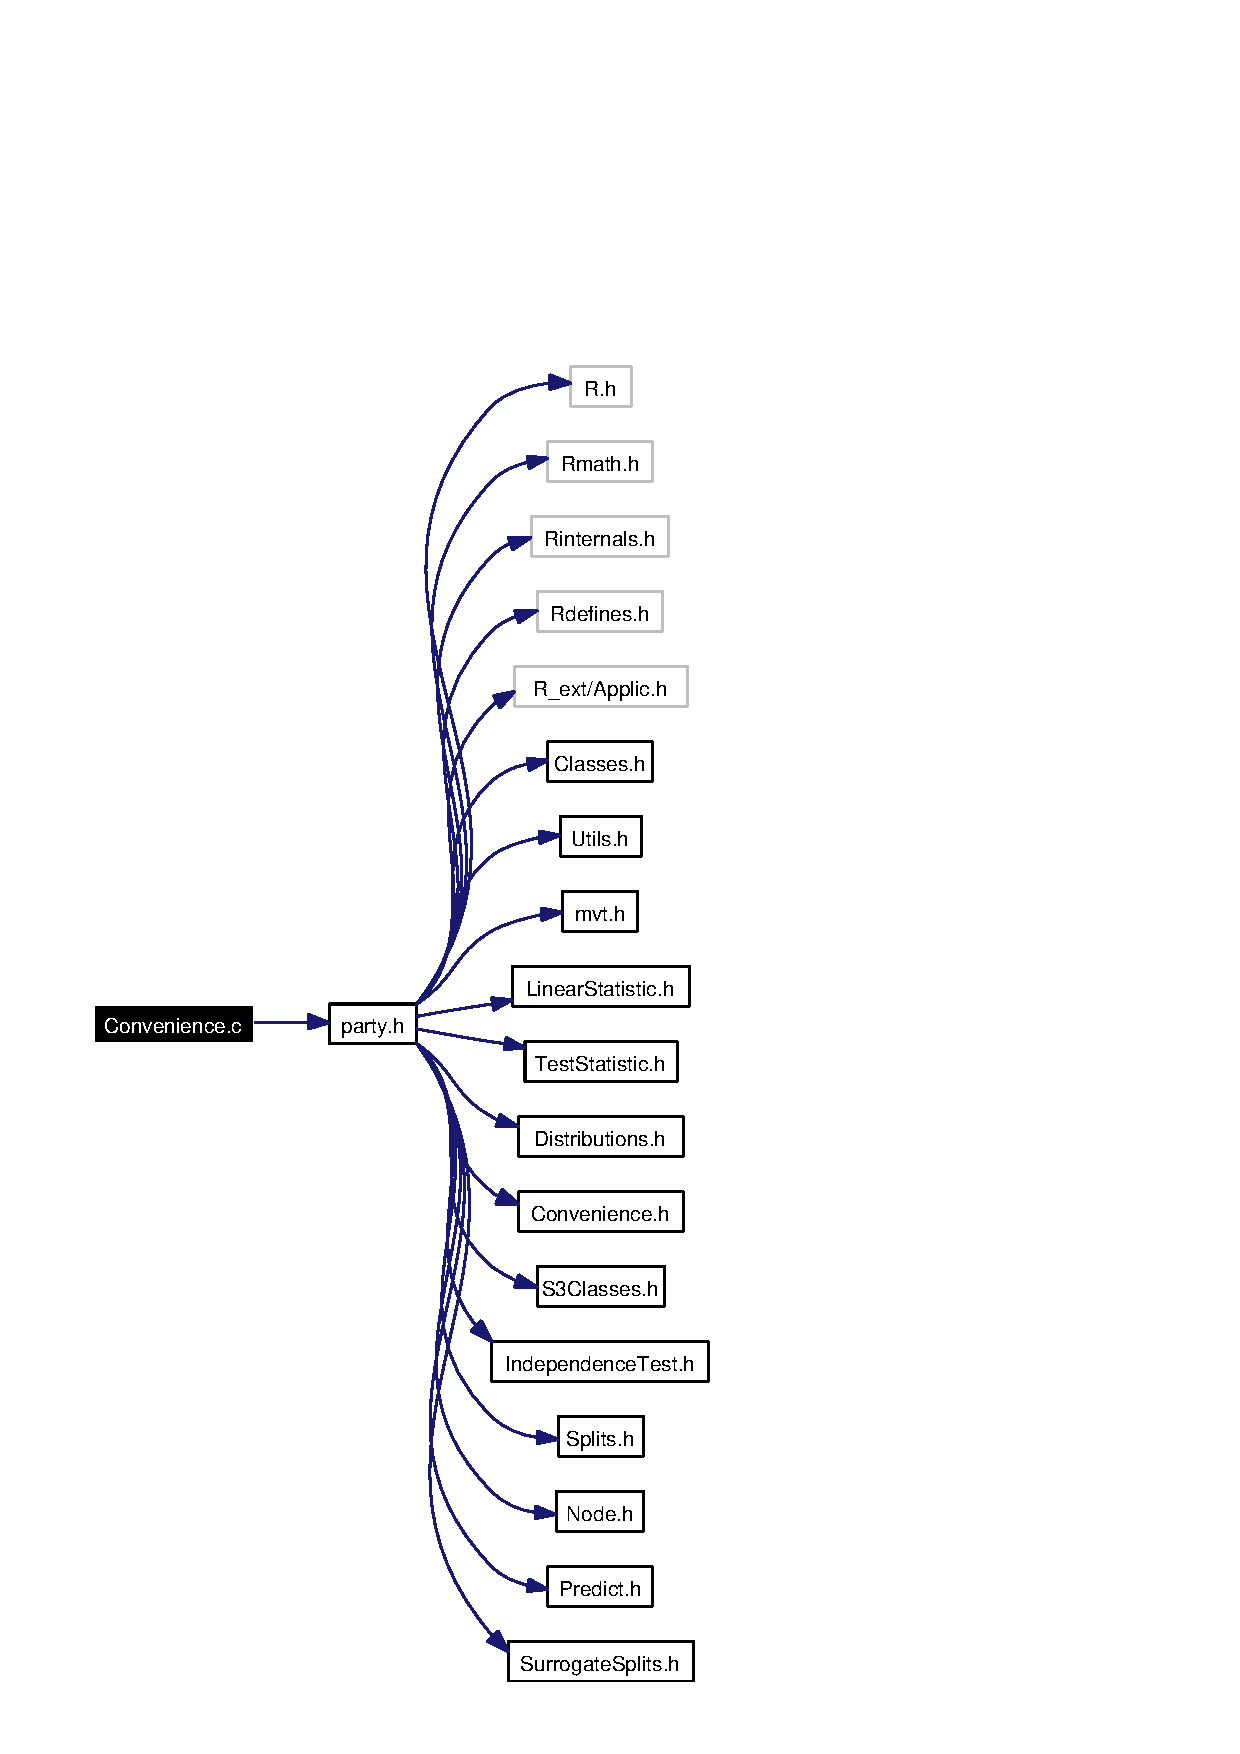
\includegraphics[width=174pt]{Convenience_8c__incl}
\end{center}
\end{figure}
\subsection*{Functions}
\begin{CompactItemize}
\item 
void \hyperlink{Convenience_8c_8d5dcca68051449e29f3b857d375c4a0}{C\_\-Lin\-Stat\-Exp\-Cov} (const double $\ast$x, const int p, const double $\ast$y, const int q, const double $\ast$weights, const int n, const int cexpcovinf, SEXP expcovinf, SEXP ans)
\item 
void \hyperlink{Convenience_8c_f39bdd14f23726fdd6bf74888ffbf920}{C\_\-Lin\-Stat\-Exp\-Cov\-MPinv} (SEXP linexpcov, double tol)
\item 
double \hyperlink{Convenience_8c_26159cd74cebf8ff7073ff588864e9ab}{C\_\-Test\-Statistic} (const SEXP linexpcov, const int type, const double tol)
\item 
double \hyperlink{Convenience_8c_a1bfc91db235a3a166a39ed1e0a224d7}{C\_\-Conditional\-Pvalue} (const double tstat, SEXP linexpcov, const int type, double tol, int $\ast$maxpts, double $\ast$releps, double $\ast$abseps)
\item 
SEXP \hyperlink{Convenience_8c_5253d5c6a188d9b7a1318c91d958047d}{R\_\-get\_\-response} (SEXP learnsample)
\item 
void \hyperlink{Convenience_8c_a1e8edb4fa73a26e73bc153c45a867b0}{R\_\-set\_\-response} (SEXP learnsample, SEXP y)
\end{CompactItemize}


\subsection{Detailed Description}
Some convenience functions

\begin{Desc}
\item[Author:]\begin{Desc}
\item[Author]hothorn \end{Desc}
\end{Desc}
\begin{Desc}
\item[Date:]\begin{Desc}
\item[Date]2006-08-25 14:38:21 +0200 (Fri, 25 Aug 2006) \end{Desc}
\end{Desc}


Definition in file \hyperlink{Convenience_8c-source}{Convenience.c}.

\subsection{Function Documentation}
\hypertarget{Convenience_8c_a1bfc91db235a3a166a39ed1e0a224d7}{
\index{Convenience.c@{Convenience.c}!C_ConditionalPvalue@{C\_\-ConditionalPvalue}}
\index{C_ConditionalPvalue@{C\_\-ConditionalPvalue}!Convenience.c@{Convenience.c}}
\subsubsection[C\_\-ConditionalPvalue]{\setlength{\rightskip}{0pt plus 5cm}double C\_\-Conditional\-Pvalue (const double {\em tstat}, SEXP {\em linexpcov}, const int {\em type}, double {\em tol}, int $\ast$ {\em maxpts}, double $\ast$ {\em releps}, double $\ast$ {\em abseps})}}
\label{Convenience_8c_a1bfc91db235a3a166a39ed1e0a224d7}


Compute asymptotic conditional P-value \begin{Desc}
\item[Parameters:]
\begin{description}
\item[{\em tstat}]test statistic \item[{\em linexpcov}]an object of class `Lin\-Stat\-Expect\-Covar' \item[{\em type}]integer, 1 (maxabs) or 2 (quadform) \item[{\em tol}]tolerance \item[{\em maxpts}]argument to C\_\-maxabs\-Conditional\-Pvalue \item[{\em releps}]argument to C\_\-maxabs\-Conditional\-Pvalue \item[{\em abseps}]argument to C\_\-maxabs\-Conditional\-Pvalue \end{description}
\end{Desc}


Definition at line 99 of file Convenience.c.

References C\_\-maxabs\-Conditional\-Pvalue(), C\_\-quadform\-Conditional\-Pvalue(), get\_\-dimension(), MAXABS, PL2\_\-covariance\-Sym, PL2\_\-rank\-Sym, and QUADFORM.

Referenced by C\_\-Teststat\-Pvalue().

Here is the call graph for this function:\begin{figure}[H]
\begin{center}
\leavevmode
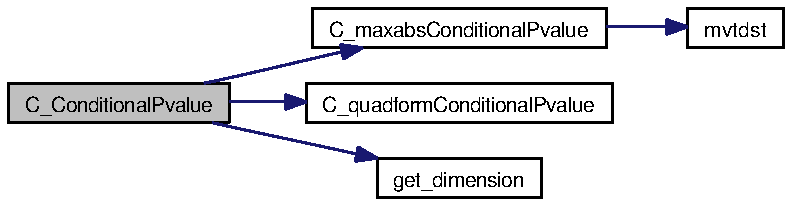
\includegraphics[width=167pt]{Convenience_8c_a1bfc91db235a3a166a39ed1e0a224d7_cgraph}
\end{center}
\end{figure}
\hypertarget{Convenience_8c_8d5dcca68051449e29f3b857d375c4a0}{
\index{Convenience.c@{Convenience.c}!C_LinStatExpCov@{C\_\-LinStatExpCov}}
\index{C_LinStatExpCov@{C\_\-LinStatExpCov}!Convenience.c@{Convenience.c}}
\subsubsection[C\_\-LinStatExpCov]{\setlength{\rightskip}{0pt plus 5cm}void C\_\-Lin\-Stat\-Exp\-Cov (const double $\ast$ {\em x}, const int {\em p}, const double $\ast$ {\em y}, const int {\em q}, const double $\ast$ {\em weights}, const int {\em n}, const int {\em cexpcovinf}, SEXP {\em expcovinf}, SEXP {\em ans})}}
\label{Convenience_8c_8d5dcca68051449e29f3b857d375c4a0}


Linear statistic of x, y, and weights and its conditional expectation and covariance \par
 \begin{Desc}
\item[Parameters:]
\begin{description}
\item[{\em x}]values of the transformation \item[{\em p}]dimension of the transformation \item[{\em y}]values of the influence function \item[{\em q}]dimension of the influence function \item[{\em weights}]case weights \item[{\em n}]number of observations \item[{\em cexpcovinf}]logical: recompute exp and cov of the influence fct \item[{\em expcovinf}]an object of class `Expect\-Covar\-Influence' \item[{\em ans}]return value; an object of class `Lin\-Stat\-Expect\-Covar' \end{description}
\end{Desc}


Definition at line 26 of file Convenience.c.

References C\_\-Expect\-Covar\-Influence(), C\_\-Expect\-Covar\-Linear\-Statistic(), C\_\-Linear\-Statistic(), and PL2\_\-linearstatistic\-Sym.

Referenced by C\_\-Independence\-Test(), and R\_\-splitcategorical().

Here is the call graph for this function:\begin{figure}[H]
\begin{center}
\leavevmode
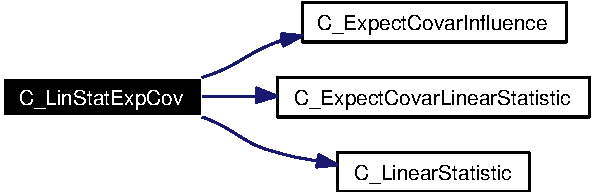
\includegraphics[width=159pt]{Convenience_8c_8d5dcca68051449e29f3b857d375c4a0_cgraph}
\end{center}
\end{figure}
\hypertarget{Convenience_8c_f39bdd14f23726fdd6bf74888ffbf920}{
\index{Convenience.c@{Convenience.c}!C_LinStatExpCovMPinv@{C\_\-LinStatExpCovMPinv}}
\index{C_LinStatExpCovMPinv@{C\_\-LinStatExpCovMPinv}!Convenience.c@{Convenience.c}}
\subsubsection[C\_\-LinStatExpCovMPinv]{\setlength{\rightskip}{0pt plus 5cm}void C\_\-Lin\-Stat\-Exp\-Cov\-MPinv (SEXP {\em linexpcov}, double {\em tol})}}
\label{Convenience_8c_f39bdd14f23726fdd6bf74888ffbf920}


Moore-Penrose inverse of the covariance matrix \par
 \begin{Desc}
\item[Parameters:]
\begin{description}
\item[{\em linexpcov}]an object of class `Lin\-Stat\-Expect\-Covar\-MPinv' \item[{\em tol}]tolerance \end{description}
\end{Desc}


Definition at line 46 of file Convenience.c.

References C\_\-MPinv(), PL2\_\-covariance\-Sym, and PL2\_\-svdmem\-Sym.

Referenced by C\_\-Independence\-Test().

Here is the call graph for this function:\begin{figure}[H]
\begin{center}
\leavevmode
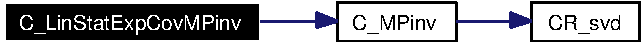
\includegraphics[width=171pt]{Convenience_8c_f39bdd14f23726fdd6bf74888ffbf920_cgraph}
\end{center}
\end{figure}
\hypertarget{Convenience_8c_26159cd74cebf8ff7073ff588864e9ab}{
\index{Convenience.c@{Convenience.c}!C_TestStatistic@{C\_\-TestStatistic}}
\index{C_TestStatistic@{C\_\-TestStatistic}!Convenience.c@{Convenience.c}}
\subsubsection[C\_\-TestStatistic]{\setlength{\rightskip}{0pt plus 5cm}double C\_\-Test\-Statistic (const SEXP {\em linexpcov}, const int {\em type}, const double {\em tol})}}
\label{Convenience_8c_26159cd74cebf8ff7073ff588864e9ab}


Compute test statistic \begin{Desc}
\item[Parameters:]
\begin{description}
\item[{\em linexpcov}]an object of class `Lin\-Stat\-Expect\-Covar' \item[{\em type}]integer, 1 (maxabs) or 2 (quadform) \item[{\em tol}]tolerance \end{description}
\end{Desc}


Definition at line 59 of file Convenience.c.

References C\_\-maxabs\-Test\-Statistic(), C\_\-quadform\-Test\-Statistic(), get\_\-dimension(), PL2\_\-covariance\-Sym, PL2\_\-expectation\-Sym, PL2\_\-linearstatistic\-Sym, and PL2\_\-MPinv\-Sym.

Referenced by C\_\-Teststat\-Pvalue().

Here is the call graph for this function:\begin{figure}[H]
\begin{center}
\leavevmode
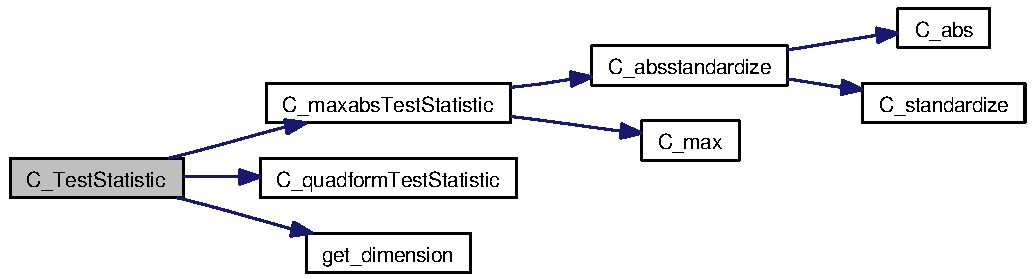
\includegraphics[width=267pt]{Convenience_8c_26159cd74cebf8ff7073ff588864e9ab_cgraph}
\end{center}
\end{figure}
\hypertarget{Convenience_8c_5253d5c6a188d9b7a1318c91d958047d}{
\index{Convenience.c@{Convenience.c}!R_get_response@{R\_\-get\_\-response}}
\index{R_get_response@{R\_\-get\_\-response}!Convenience.c@{Convenience.c}}
\subsubsection[R\_\-get\_\-response]{\setlength{\rightskip}{0pt plus 5cm}SEXP R\_\-get\_\-response (SEXP {\em learnsample})}}
\label{Convenience_8c_5253d5c6a188d9b7a1318c91d958047d}


extract the (first) response variable from a learning sample \begin{Desc}
\item[Parameters:]
\begin{description}
\item[{\em learnsample}]an object of class `Learning\-Sample' \end{description}
\end{Desc}


Definition at line 131 of file Convenience.c.

References PL2\_\-responses\-Sym, and PL2\_\-variables\-Sym.

Referenced by R\_\-set\_\-response().\hypertarget{Convenience_8c_a1e8edb4fa73a26e73bc153c45a867b0}{
\index{Convenience.c@{Convenience.c}!R_set_response@{R\_\-set\_\-response}}
\index{R_set_response@{R\_\-set\_\-response}!Convenience.c@{Convenience.c}}
\subsubsection[R\_\-set\_\-response]{\setlength{\rightskip}{0pt plus 5cm}void R\_\-set\_\-response (SEXP {\em learnsample}, SEXP {\em y})}}
\label{Convenience_8c_a1e8edb4fa73a26e73bc153c45a867b0}


change the values of the response variable in a learning sample \begin{Desc}
\item[Parameters:]
\begin{description}
\item[{\em learnsample}]an object of class `Learning\-Sample' \item[{\em y}]a REAL with new values \end{description}
\end{Desc}


Definition at line 143 of file Convenience.c.

References PL2\_\-jointtransf\-Sym, PL2\_\-responses\-Sym, PL2\_\-transformations\-Sym, PL2\_\-variables\-Sym, and R\_\-get\_\-response().

Here is the call graph for this function:\begin{figure}[H]
\begin{center}
\leavevmode
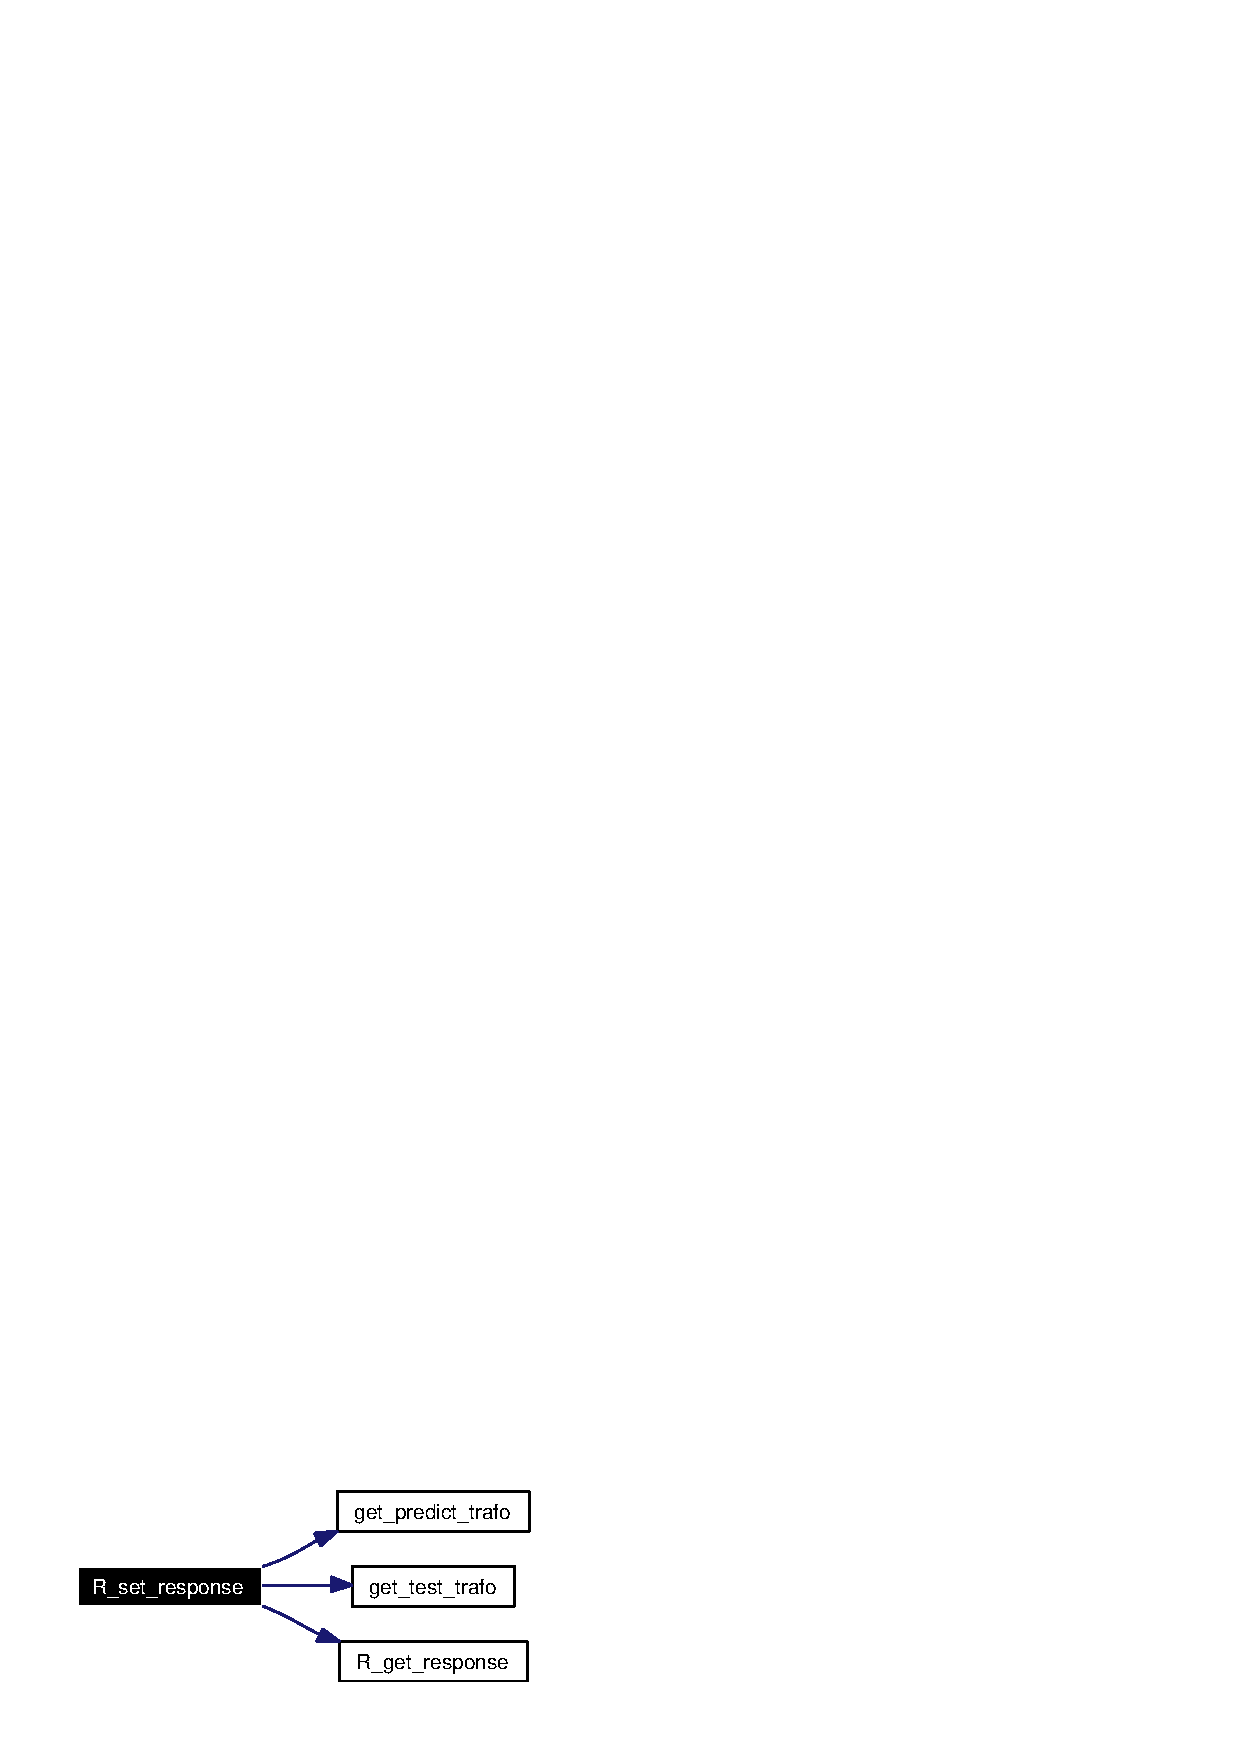
\includegraphics[width=126pt]{Convenience_8c_a1e8edb4fa73a26e73bc153c45a867b0_cgraph}
\end{center}
\end{figure}

\hypertarget{Convenience_8h}{
\section{Convenience.h File Reference}
\label{Convenience_8h}\index{Convenience.h@{Convenience.h}}
}


This graph shows which files directly or indirectly include this file:\begin{figure}[H]
\begin{center}
\leavevmode
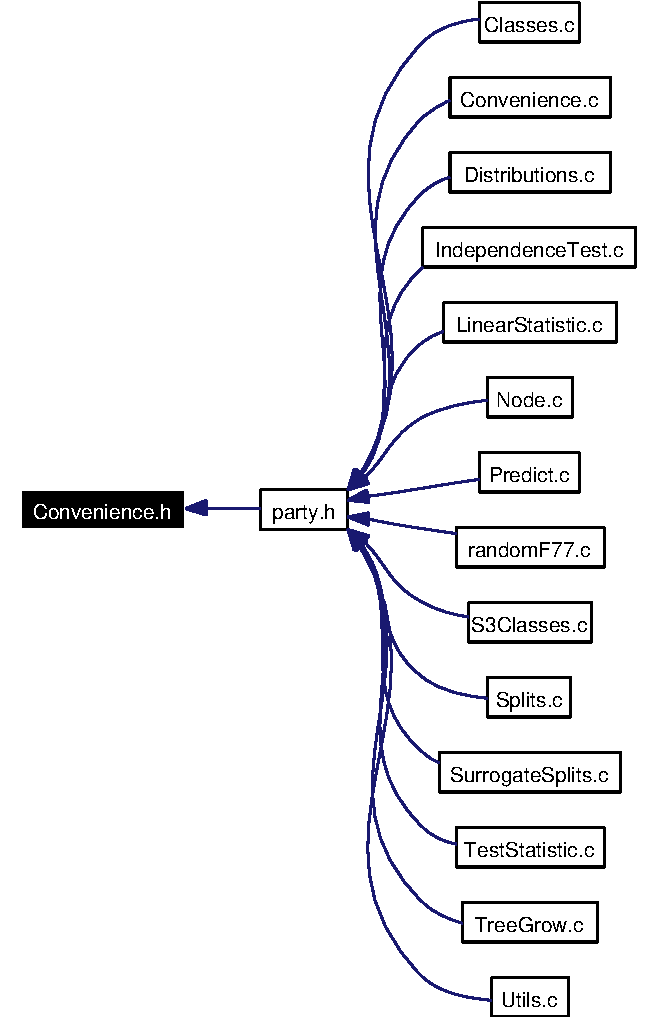
\includegraphics[width=173pt]{Convenience_8h__dep__incl}
\end{center}
\end{figure}
\subsection*{Functions}
\begin{CompactItemize}
\item 
void \hyperlink{Convenience_8h_a0}{C\_\-Lin\-Stat\-Exp\-Cov} (const double $\ast$x, const int p, const double $\ast$y, const int q, const double $\ast$weights, const int n, const int cexpcovinf, SEXP expcovinf, SEXP ans)
\item 
void \hyperlink{Convenience_8h_a1}{C\_\-Lin\-Stat\-Exp\-Cov\-MPinv} (SEXP linexpcov, double tol)
\item 
void \hyperlink{Convenience_8h_a2}{C\_\-MLinear\-Statistic} (SEXP linexpcov, SEXP Score\-Matrix, SEXP ans)
\item 
double \hyperlink{Convenience_8h_a3}{C\_\-Test\-Statistic} (const SEXP linexpcov, const int type, const double tol)
\item 
double \hyperlink{Convenience_8h_a4}{C\_\-Conditional\-Pvalue} (const double tstat, SEXP linexpcov, const int type, double tol, int $\ast$maxpts, double $\ast$releps, double $\ast$abseps)
\end{CompactItemize}


\subsection{Function Documentation}
\hypertarget{Convenience_8h_a4}{
\index{Convenience.h@{Convenience.h}!C_ConditionalPvalue@{C\_\-ConditionalPvalue}}
\index{C_ConditionalPvalue@{C\_\-ConditionalPvalue}!Convenience.h@{Convenience.h}}
\subsubsection[C\_\-ConditionalPvalue]{\setlength{\rightskip}{0pt plus 5cm}double C\_\-Conditional\-Pvalue (const double {\em tstat}, SEXP {\em linexpcov}, const int {\em type}, double {\em tol}, int $\ast$ {\em maxpts}, double $\ast$ {\em releps}, double $\ast$ {\em abseps})}}
\label{Convenience_8h_a4}


Compute asymptotic conditional P-value \begin{Desc}
\item[Parameters:]
\begin{description}
\item[{\em tstat}]test statistic \item[{\em linexpcov}]an object of class `Lin\-Stat\-Expect\-Covar' \item[{\em type}]integer, 1 (maxabs) or 2 (quadform) \item[{\em tol}]tolerance \item[{\em maxpts}]argument to C\_\-maxabs\-Conditional\-Pvalue \item[{\em releps}]argument to C\_\-maxabs\-Conditional\-Pvalue \item[{\em abseps}]argument to C\_\-maxabs\-Conditional\-Pvalue\end{description}
\end{Desc}


Definition at line 131 of file Convenience.c.

References C\_\-maxabs\-Conditional\-Pvalue(), C\_\-quadform\-Conditional\-Pvalue(), get\_\-dimension(), MAXABS, PL2\_\-covariance\-Sym, PL2\_\-rank\-Sym, and QUADFORM.

Referenced by C\_\-Teststat\-Pvalue().

Here is the call graph for this function:\begin{figure}[H]
\begin{center}
\leavevmode
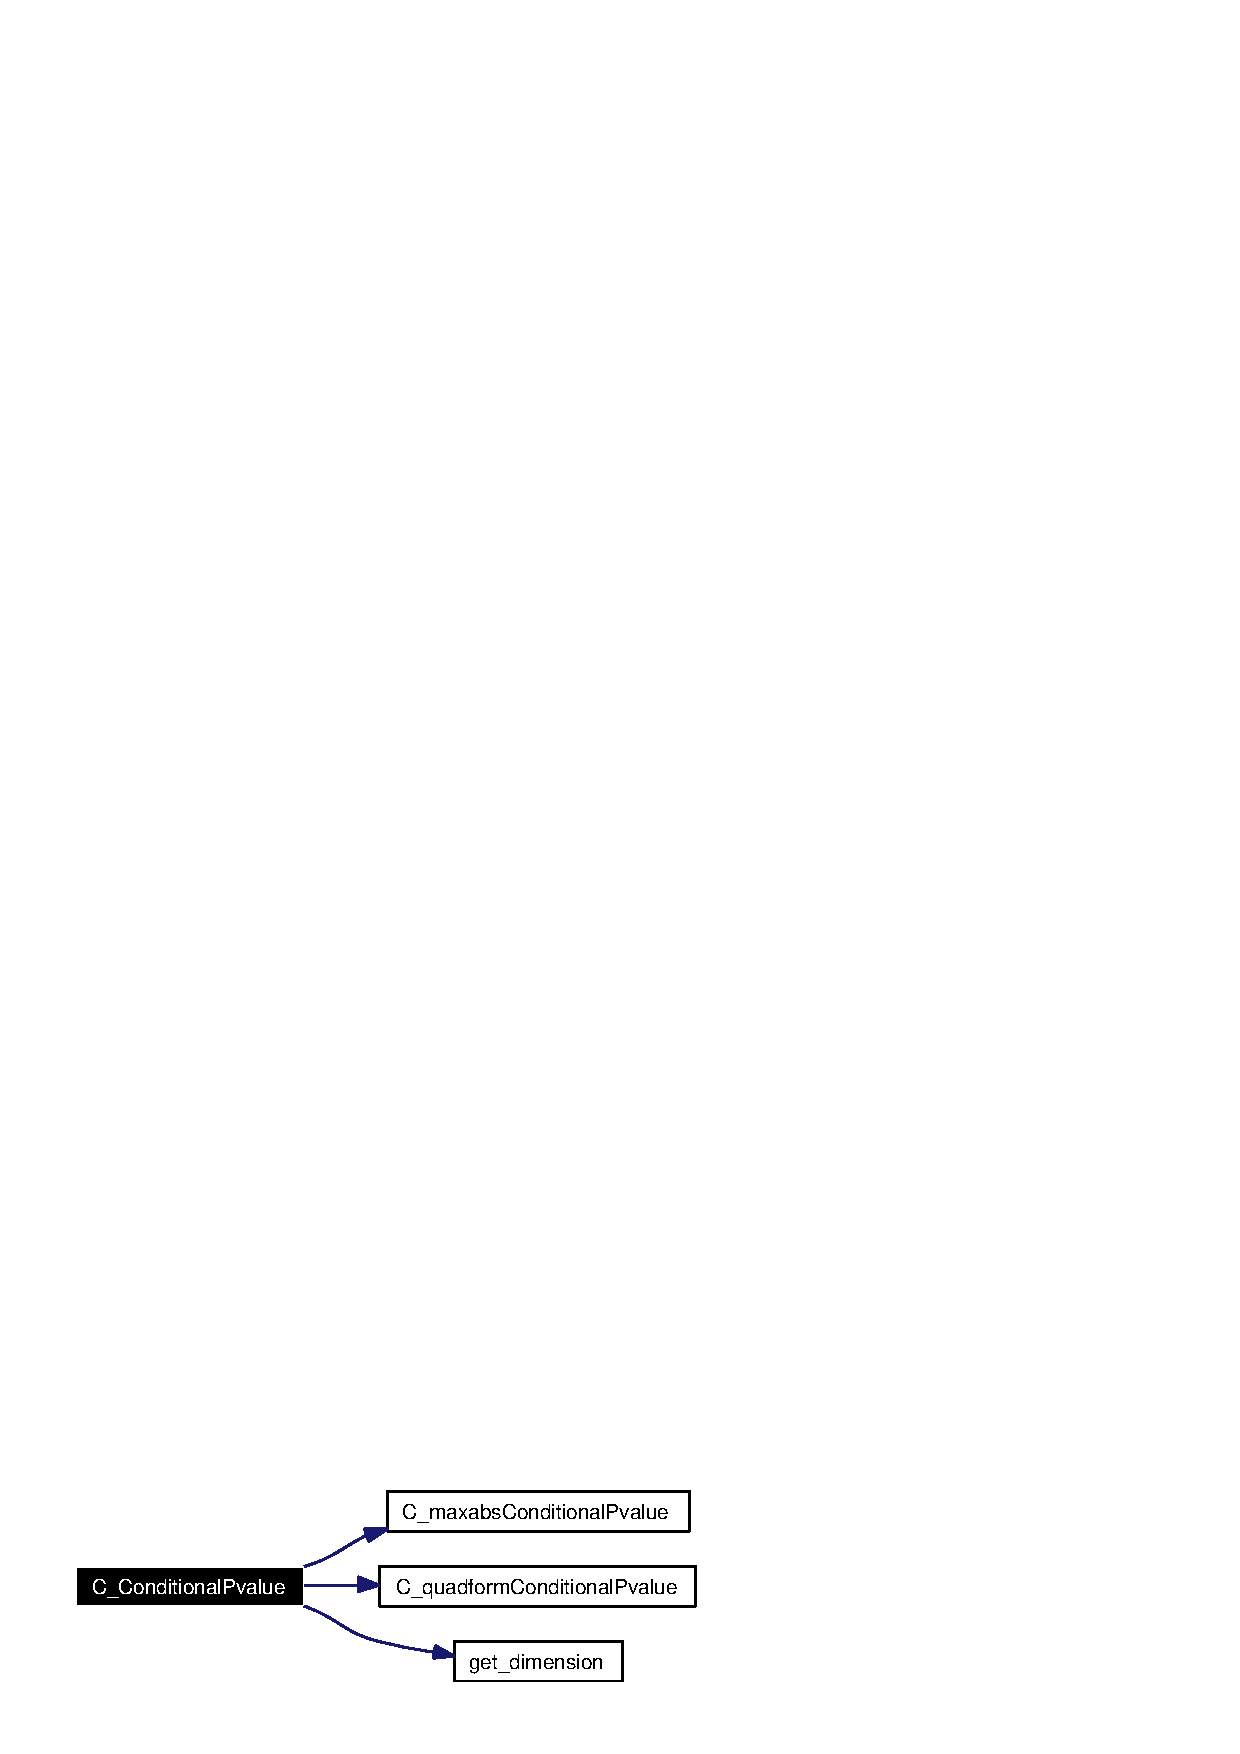
\includegraphics[width=167pt]{Convenience_8h_a4_cgraph}
\end{center}
\end{figure}
\hypertarget{Convenience_8h_a0}{
\index{Convenience.h@{Convenience.h}!C_LinStatExpCov@{C\_\-LinStatExpCov}}
\index{C_LinStatExpCov@{C\_\-LinStatExpCov}!Convenience.h@{Convenience.h}}
\subsubsection[C\_\-LinStatExpCov]{\setlength{\rightskip}{0pt plus 5cm}void C\_\-Lin\-Stat\-Exp\-Cov (const double $\ast$ {\em x}, const int {\em p}, const double $\ast$ {\em y}, const int {\em q}, const double $\ast$ {\em weights}, const int {\em n}, const int {\em cexpcovinf}, SEXP {\em expcovinf}, SEXP {\em ans})}}
\label{Convenience_8h_a0}


Linear statistic of x, y, and weights and its conditional expectation and covariance \par
 \begin{Desc}
\item[Parameters:]
\begin{description}
\item[{\em x}]values of the transformation \item[{\em p}]dimension of the transformation \item[{\em y}]values of the influence function \item[{\em q}]dimension of the influence function \item[{\em weights}]case weights \item[{\em n}]number of observations \item[{\em cexpcovinf}]logical: recompute exp and cov of the influence fct \item[{\em expcovinf}]an object of class `Expect\-Covar\-Influence' \item[{\em ans}]return value; an object of class `Lin\-Stat\-Expect\-Covar'\end{description}
\end{Desc}


Definition at line 26 of file Convenience.c.

References C\_\-Expect\-Covar\-Influence(), C\_\-Expect\-Covar\-Linear\-Statistic(), C\_\-Linear\-Statistic(), and PL2\_\-linearstatistic\-Sym.

Referenced by C\_\-Global\-Test(), C\_\-Independence\-Test(), and R\_\-splitcategorical().

Here is the call graph for this function:\begin{figure}[H]
\begin{center}
\leavevmode
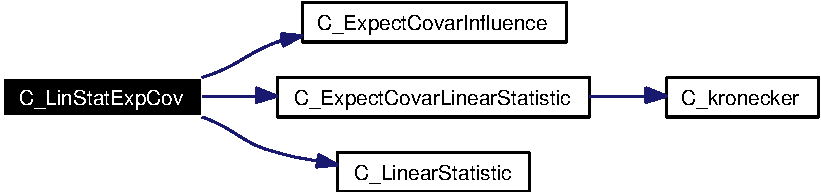
\includegraphics[width=214pt]{Convenience_8h_a0_cgraph}
\end{center}
\end{figure}
\hypertarget{Convenience_8h_a1}{
\index{Convenience.h@{Convenience.h}!C_LinStatExpCovMPinv@{C\_\-LinStatExpCovMPinv}}
\index{C_LinStatExpCovMPinv@{C\_\-LinStatExpCovMPinv}!Convenience.h@{Convenience.h}}
\subsubsection[C\_\-LinStatExpCovMPinv]{\setlength{\rightskip}{0pt plus 5cm}void C\_\-Lin\-Stat\-Exp\-Cov\-MPinv (SEXP {\em linexpcov}, double {\em tol})}}
\label{Convenience_8h_a1}


Moore-Penrose inverse of the covariance matrix \par
 \begin{Desc}
\item[Parameters:]
\begin{description}
\item[{\em linexpcov}]an object of class `Lin\-Stat\-Expect\-Covar\-MPinv' \item[{\em tol}]tolerance\end{description}
\end{Desc}


Definition at line 46 of file Convenience.c.

References C\_\-MPinv(), PL2\_\-covariance\-Sym, and PL2\_\-svdmem\-Sym.

Referenced by C\_\-Global\-Test(), and C\_\-Independence\-Test().

Here is the call graph for this function:\begin{figure}[H]
\begin{center}
\leavevmode
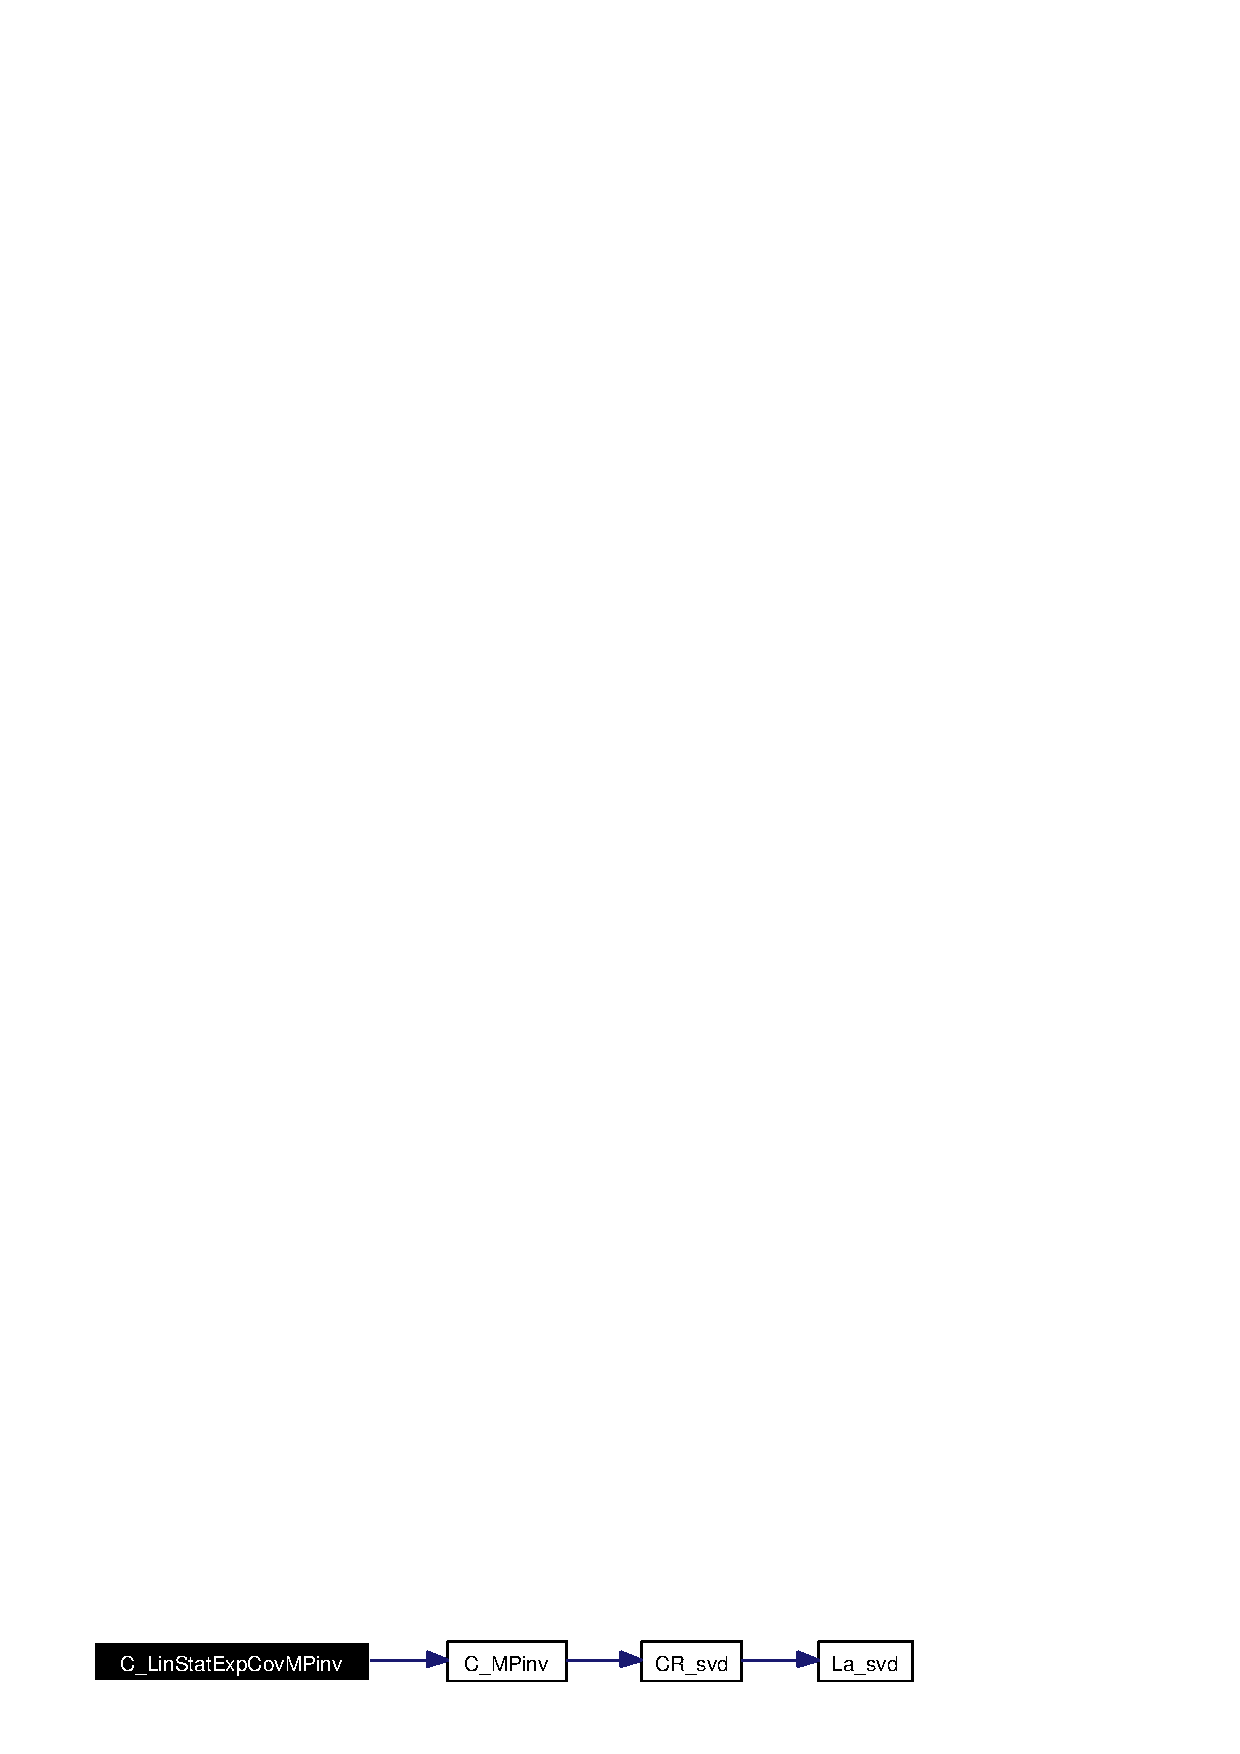
\includegraphics[width=214pt]{Convenience_8h_a1_cgraph}
\end{center}
\end{figure}
\hypertarget{Convenience_8h_a2}{
\index{Convenience.h@{Convenience.h}!C_MLinearStatistic@{C\_\-MLinearStatistic}}
\index{C_MLinearStatistic@{C\_\-MLinearStatistic}!Convenience.h@{Convenience.h}}
\subsubsection[C\_\-MLinearStatistic]{\setlength{\rightskip}{0pt plus 5cm}void C\_\-MLinear\-Statistic (SEXP {\em linexpcov}, SEXP {\em Score\-Matrix}, SEXP {\em ans})}}
\label{Convenience_8h_a2}


Linear combination of a linear statistic, expectation and covariance \begin{Desc}
\item[Parameters:]
\begin{description}
\item[{\em linexpcov}]an object of class `Lin\-Stat\-Expect\-Covar' \item[{\em Score\-Matrix}]matrix of coefficients \item[{\em ans}]return value; an object of class `Lin\-Stat\-Expect\-Covar'\end{description}
\end{Desc}


Definition at line 59 of file Convenience.c.

References C\_\-matprod(), C\_\-matprod\-T(), get\_\-dimension(), ncol(), nrow(), PL2\_\-covariance\-Sym, PL2\_\-expectation\-Sym, and PL2\_\-linearstatistic\-Sym.

Referenced by C\_\-Global\-Test(), C\_\-Independence\-Test(), and C\_\-Monte\-Carlo().

Here is the call graph for this function:\begin{figure}[H]
\begin{center}
\leavevmode
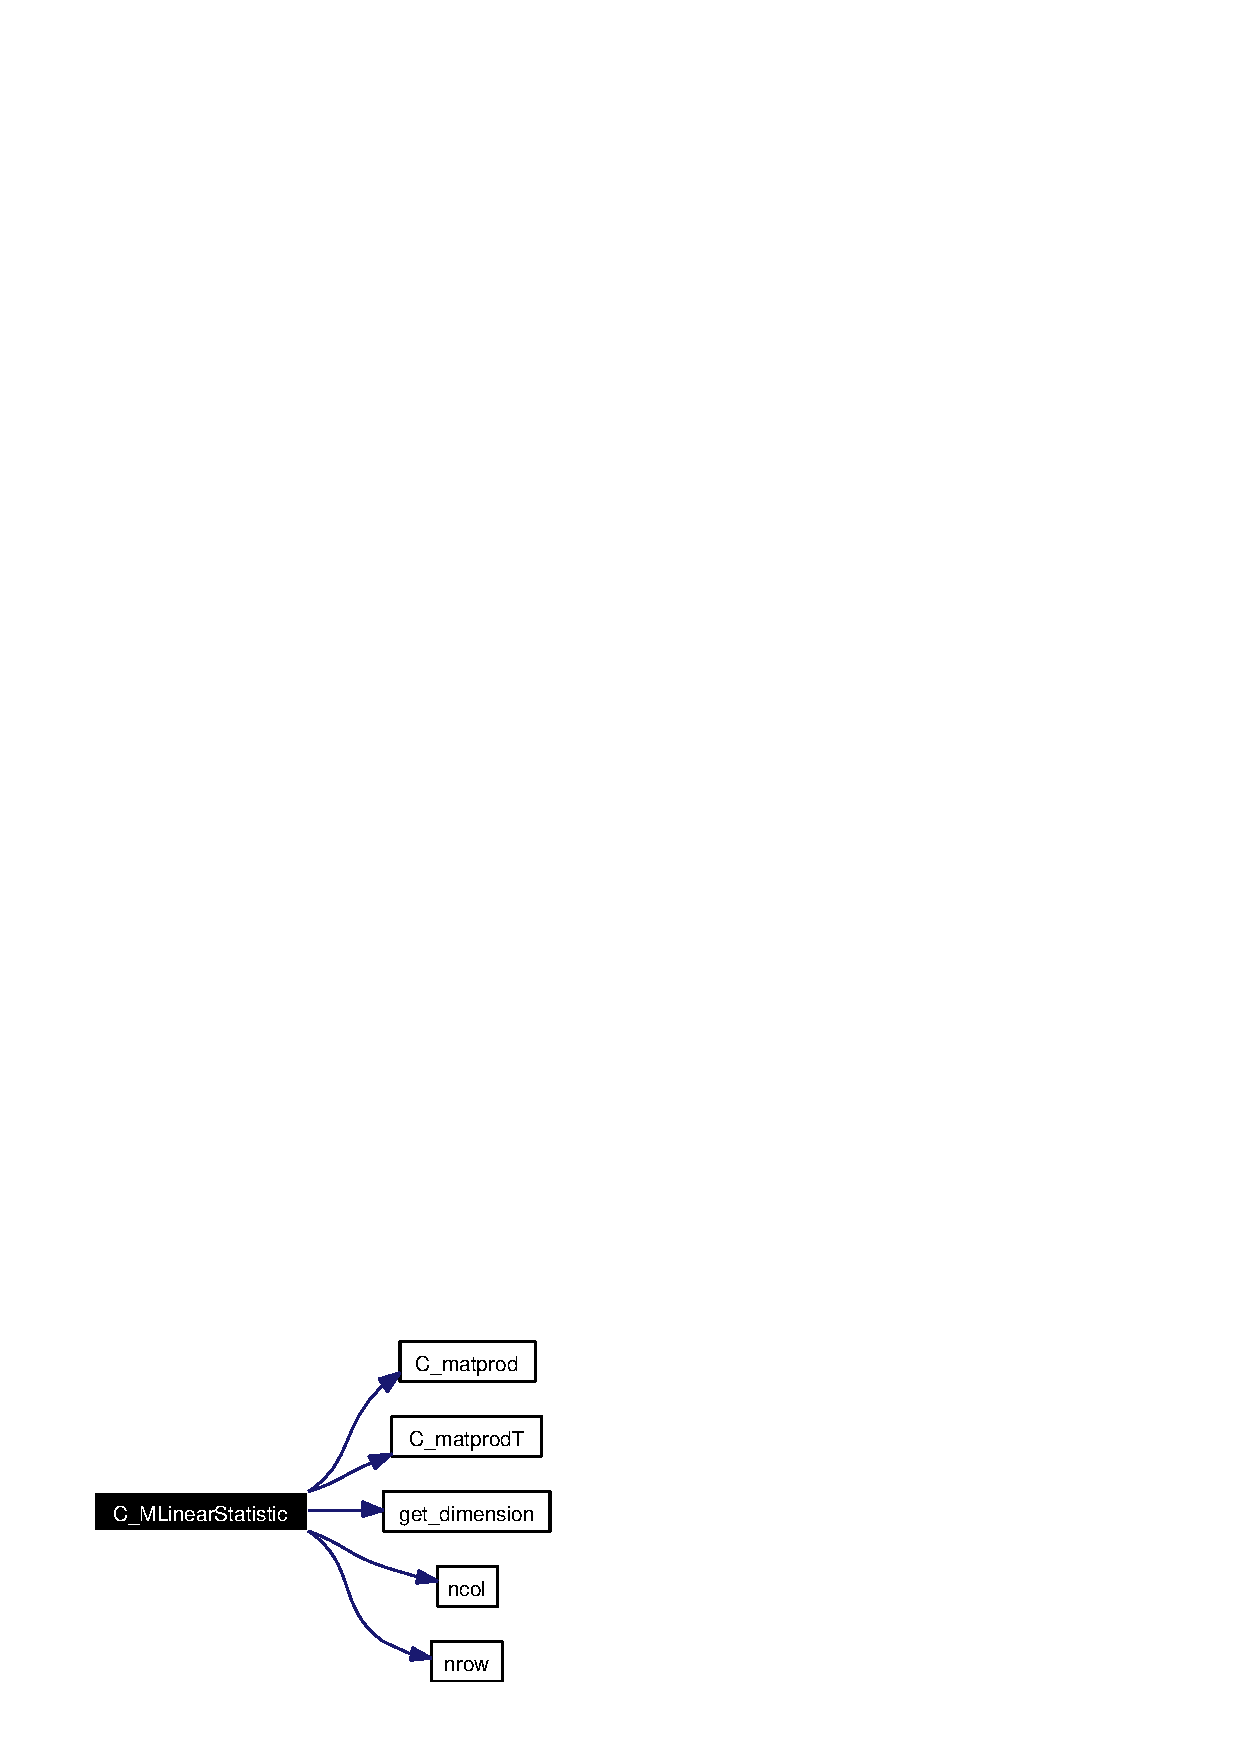
\includegraphics[width=128pt]{Convenience_8h_a2_cgraph}
\end{center}
\end{figure}
\hypertarget{Convenience_8h_a3}{
\index{Convenience.h@{Convenience.h}!C_TestStatistic@{C\_\-TestStatistic}}
\index{C_TestStatistic@{C\_\-TestStatistic}!Convenience.h@{Convenience.h}}
\subsubsection[C\_\-TestStatistic]{\setlength{\rightskip}{0pt plus 5cm}double C\_\-Test\-Statistic (const SEXP {\em linexpcov}, const int {\em type}, const double {\em tol})}}
\label{Convenience_8h_a3}


Compute test statistic \begin{Desc}
\item[Parameters:]
\begin{description}
\item[{\em linexpcov}]an object of class `Lin\-Stat\-Expect\-Covar' \item[{\em type}]integer, 1 (maxabs) or 2 (quadform) \item[{\em tol}]tolerance\end{description}
\end{Desc}


Definition at line 91 of file Convenience.c.

References C\_\-maxabs\-Test\-Statistic(), C\_\-quadform\-Test\-Statistic(), get\_\-dimension(), PL2\_\-covariance\-Sym, PL2\_\-expectation\-Sym, PL2\_\-linearstatistic\-Sym, and PL2\_\-MPinv\-Sym.

Referenced by C\_\-Teststat\-Pvalue().

Here is the call graph for this function:\begin{figure}[H]
\begin{center}
\leavevmode
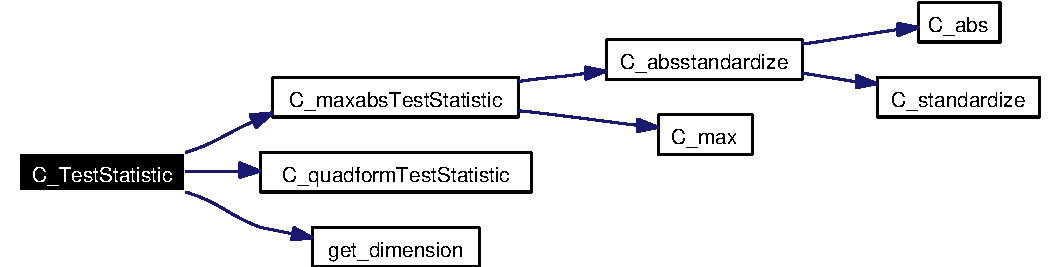
\includegraphics[width=267pt]{Convenience_8h_a3_cgraph}
\end{center}
\end{figure}

\hypertarget{Distributions_8c}{
\section{Distributions.c File Reference}
\label{Distributions_8c}\index{Distributions.c@{Distributions.c}}
}
{\tt \#include \char`\"{}party.h\char`\"{}}\par


Include dependency graph for Distributions.c:\begin{figure}[H]
\begin{center}
\leavevmode
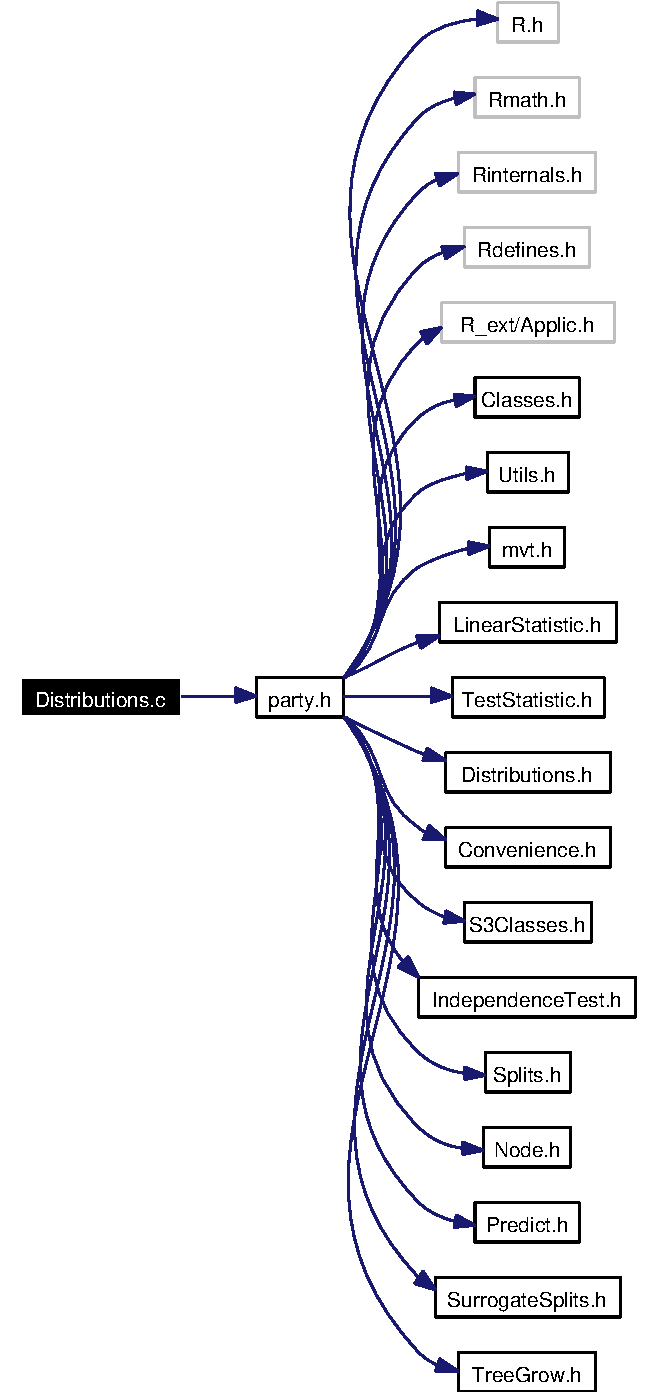
\includegraphics[width=172pt]{Distributions_8c__incl}
\end{center}
\end{figure}
\subsection*{Functions}
\begin{CompactItemize}
\item 
double \hyperlink{Distributions_8c_a0}{C\_\-quadform\-Conditional\-Pvalue} (const double tstat, const double df)
\item 
SEXP \hyperlink{Distributions_8c_a1}{R\_\-quadform\-Conditional\-Pvalue} (SEXP tstat, SEXP df)
\item 
double \hyperlink{Distributions_8c_a2}{C\_\-maxabs\-Conditional\-Pvalue} (const double tstat, const double $\ast$Sigma, const int pq, int $\ast$maxpts, double $\ast$releps, double $\ast$abseps, double $\ast$tol)
\item 
SEXP \hyperlink{Distributions_8c_a3}{R\_\-maxabs\-Conditional\-Pvalue} (SEXP tstat, SEXP Sigma, SEXP maxpts, SEXP releps, SEXP abseps, SEXP tol)
\item 
void \hyperlink{Distributions_8c_a4}{C\_\-Monte\-Carlo} (double $\ast$criterion, SEXP learnsample, SEXP weights, SEXP fitmem, SEXP varctrl, SEXP gtctrl, double $\ast$ans\_\-pvalues)
\item 
SEXP \hyperlink{Distributions_8c_a5}{R\_\-Monte\-Carlo} (SEXP criterion, SEXP learnsample, SEXP weights, SEXP fitmem, SEXP varctrl, SEXP gtctrl)
\end{CompactItemize}


\subsection{Detailed Description}
Conditional Distributions

\begin{Desc}
\item[Author:]\begin{Desc}
\item[Author]hothorn \end{Desc}
\end{Desc}
\begin{Desc}
\item[Date:]\begin{Desc}
\item[Date]2005/07/07 12:32:01 \end{Desc}
\end{Desc}


Definition in file \hyperlink{Distributions_8c-source}{Distributions.c}.

\subsection{Function Documentation}
\hypertarget{Distributions_8c_a2}{
\index{Distributions.c@{Distributions.c}!C_maxabsConditionalPvalue@{C\_\-maxabsConditionalPvalue}}
\index{C_maxabsConditionalPvalue@{C\_\-maxabsConditionalPvalue}!Distributions.c@{Distributions.c}}
\subsubsection[C\_\-maxabsConditionalPvalue]{\setlength{\rightskip}{0pt plus 5cm}double C\_\-maxabs\-Conditional\-Pvalue (const double {\em tstat}, const double $\ast$ {\em Sigma}, const int {\em pq}, int $\ast$ {\em maxpts}, double $\ast$ {\em releps}, double $\ast$ {\em abseps}, double $\ast$ {\em tol})}}
\label{Distributions_8c_a2}


Conditional asymptotic P-value of a maxabs-type test statistic\par
 Basically the functionality from package `mvtnorm' \par
 \begin{Desc}
\item[Parameters:]
\begin{description}
\item[{\em tstat}]test statitstic \item[{\em Sigma}]covariance matrix \item[{\em pq}]nrow(Sigma) \item[{\em maxpts}]number of Monte-Carlo steps \item[{\em releps}]relative error \item[{\em abseps}]absolute error \item[{\em tol}]tolerance \end{description}
\end{Desc}


Definition at line 52 of file Distributions.c.

References mvtdst.

Referenced by C\_\-Conditional\-Pvalue(), and R\_\-maxabs\-Conditional\-Pvalue().\hypertarget{Distributions_8c_a4}{
\index{Distributions.c@{Distributions.c}!C_MonteCarlo@{C\_\-MonteCarlo}}
\index{C_MonteCarlo@{C\_\-MonteCarlo}!Distributions.c@{Distributions.c}}
\subsubsection[C\_\-MonteCarlo]{\setlength{\rightskip}{0pt plus 5cm}void C\_\-Monte\-Carlo (double $\ast$ {\em criterion}, SEXP {\em learnsample}, SEXP {\em weights}, SEXP {\em fitmem}, SEXP {\em varctrl}, SEXP {\em gtctrl}, double $\ast$ {\em ans\_\-pvalues})}}
\label{Distributions_8c_a4}


Monte-Carlo approximation to the conditional pvalues \begin{Desc}
\item[Parameters:]
\begin{description}
\item[{\em criterion}]vector of node criteria for each input \item[{\em learnsample}]an object of class `Learning\-Sample' \item[{\em weights}]case weights \item[{\em fitmem}]an object of class `Tree\-Fit\-Memory' \item[{\em varctrl}]an object of class `Variable\-Control' \item[{\em gtctrl}]an object of class `Global\-Test\-Control' \item[{\em ans\_\-pvalues}]return values; vector of adjusted pvalues \end{description}
\end{Desc}


Definition at line 169 of file Distributions.c.

References C\_\-Linear\-Statistic(), C\_\-max(), C\_\-MLinear\-Statistic(), C\_\-Permuted\-Linear\-Statistic(), C\_\-Sample\-No\-Replace(), C\_\-Teststat\-Criterion(), get\_\-Mscorematrix(), get\_\-ninputs(), get\_\-nobs(), get\_\-nresample(), get\_\-transformation(), get\_\-varmemory(), get\_\-var\-Mmemory(), has\_\-missings(), is\_\-ordinal(), ncol(), PL2\_\-expcovinf\-Sym, PL2\_\-inputs\-Sym, PL2\_\-linearstatistic\-Sym, PL2\_\-responses\-Sym, and PL2\_\-sumweights\-Sym.

Referenced by C\_\-Global\-Test(), and R\_\-Monte\-Carlo().

Here is the call graph for this function:\begin{figure}[H]
\begin{center}
\leavevmode
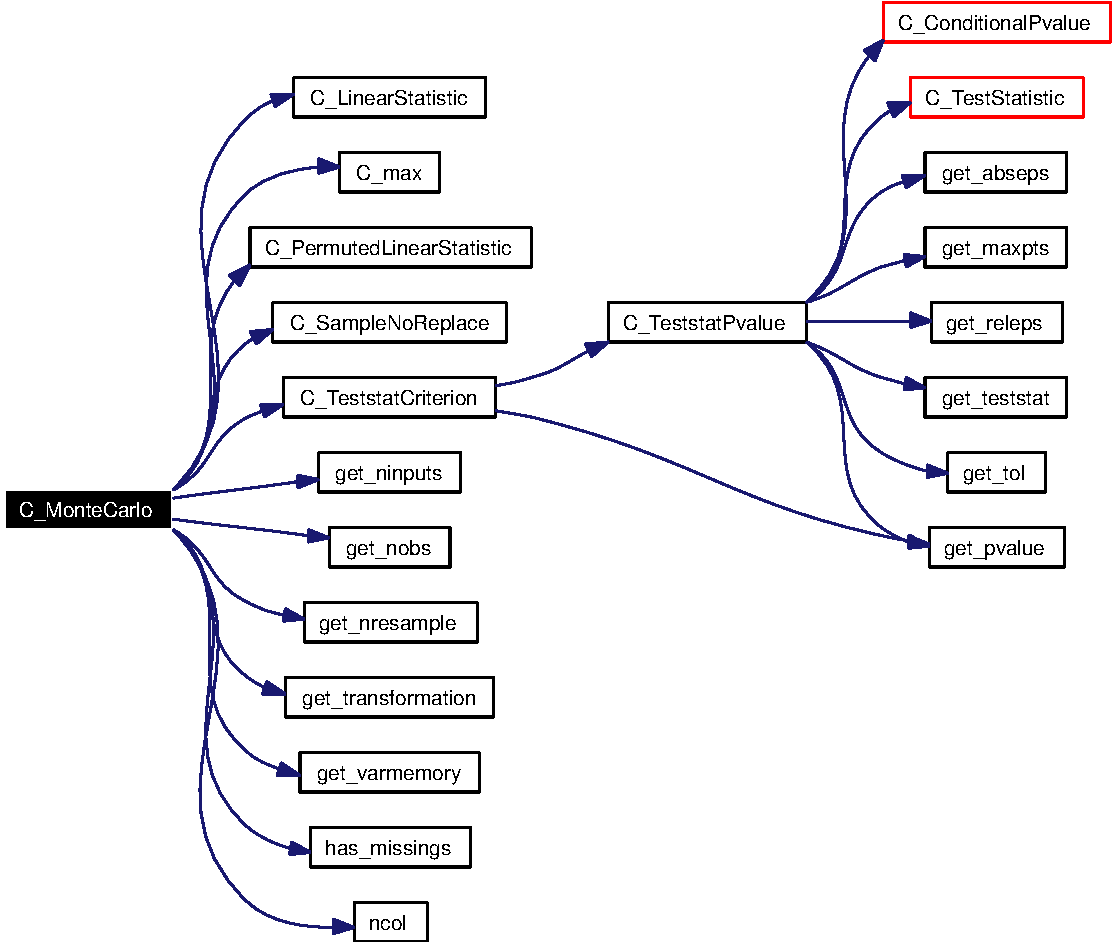
\includegraphics[width=343pt]{Distributions_8c_a4_cgraph}
\end{center}
\end{figure}
\hypertarget{Distributions_8c_a0}{
\index{Distributions.c@{Distributions.c}!C_quadformConditionalPvalue@{C\_\-quadformConditionalPvalue}}
\index{C_quadformConditionalPvalue@{C\_\-quadformConditionalPvalue}!Distributions.c@{Distributions.c}}
\subsubsection[C\_\-quadformConditionalPvalue]{\setlength{\rightskip}{0pt plus 5cm}double C\_\-quadform\-Conditional\-Pvalue (const double {\em tstat}, const double {\em df})}}
\label{Distributions_8c_a0}


Conditional asymptotic P-value of a quadratic form\par
 \begin{Desc}
\item[Parameters:]
\begin{description}
\item[{\em tstat}]test statistic \item[{\em df}]degree of freedom \end{description}
\end{Desc}


Definition at line 18 of file Distributions.c.

Referenced by C\_\-Conditional\-Pvalue(), and R\_\-quadform\-Conditional\-Pvalue().\hypertarget{Distributions_8c_a3}{
\index{Distributions.c@{Distributions.c}!R_maxabsConditionalPvalue@{R\_\-maxabsConditionalPvalue}}
\index{R_maxabsConditionalPvalue@{R\_\-maxabsConditionalPvalue}!Distributions.c@{Distributions.c}}
\subsubsection[R\_\-maxabsConditionalPvalue]{\setlength{\rightskip}{0pt plus 5cm}SEXP R\_\-maxabs\-Conditional\-Pvalue (SEXP {\em tstat}, SEXP {\em Sigma}, SEXP {\em maxpts}, SEXP {\em releps}, SEXP {\em abseps}, SEXP {\em tol})}}
\label{Distributions_8c_a3}


R-interface to C\_\-maxabs\-Conditional\-Pvalue \par
 \begin{Desc}
\item[Parameters:]
\begin{description}
\item[{\em tstat}]test statitstic \item[{\em Sigma}]covariance matrix \item[{\em maxpts}]number of Monte-Carlo steps \item[{\em releps}]relative error \item[{\em abseps}]absolute error \item[{\em tol}]tolerance \end{description}
\end{Desc}


Definition at line 142 of file Distributions.c.

References C\_\-maxabs\-Conditional\-Pvalue(), and nrow().

Here is the call graph for this function:\begin{figure}[H]
\begin{center}
\leavevmode
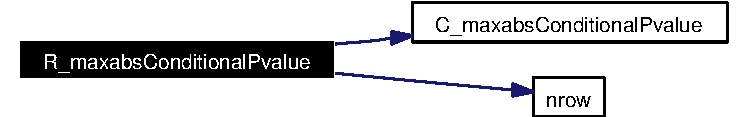
\includegraphics[width=182pt]{Distributions_8c_a3_cgraph}
\end{center}
\end{figure}
\hypertarget{Distributions_8c_a5}{
\index{Distributions.c@{Distributions.c}!R_MonteCarlo@{R\_\-MonteCarlo}}
\index{R_MonteCarlo@{R\_\-MonteCarlo}!Distributions.c@{Distributions.c}}
\subsubsection[R\_\-MonteCarlo]{\setlength{\rightskip}{0pt plus 5cm}SEXP R\_\-Monte\-Carlo (SEXP {\em criterion}, SEXP {\em learnsample}, SEXP {\em weights}, SEXP {\em fitmem}, SEXP {\em varctrl}, SEXP {\em gtctrl})}}
\label{Distributions_8c_a5}


R-interface to C\_\-Monte\-Carlo \par
 \begin{Desc}
\item[Parameters:]
\begin{description}
\item[{\em criterion}]vector of node criteria for each input \item[{\em learnsample}]an object of class `Learning\-Sample' \item[{\em weights}]case weights \item[{\em fitmem}]an object of class `Tree\-Fit\-Memory' \item[{\em varctrl}]an object of class `Variable\-Control' \item[{\em gtctrl}]an object of class `Global\-Test\-Control' \end{description}
\end{Desc}


Definition at line 289 of file Distributions.c.

References C\_\-Monte\-Carlo(), and get\_\-ninputs().

Here is the call graph for this function:\begin{figure}[H]
\begin{center}
\leavevmode
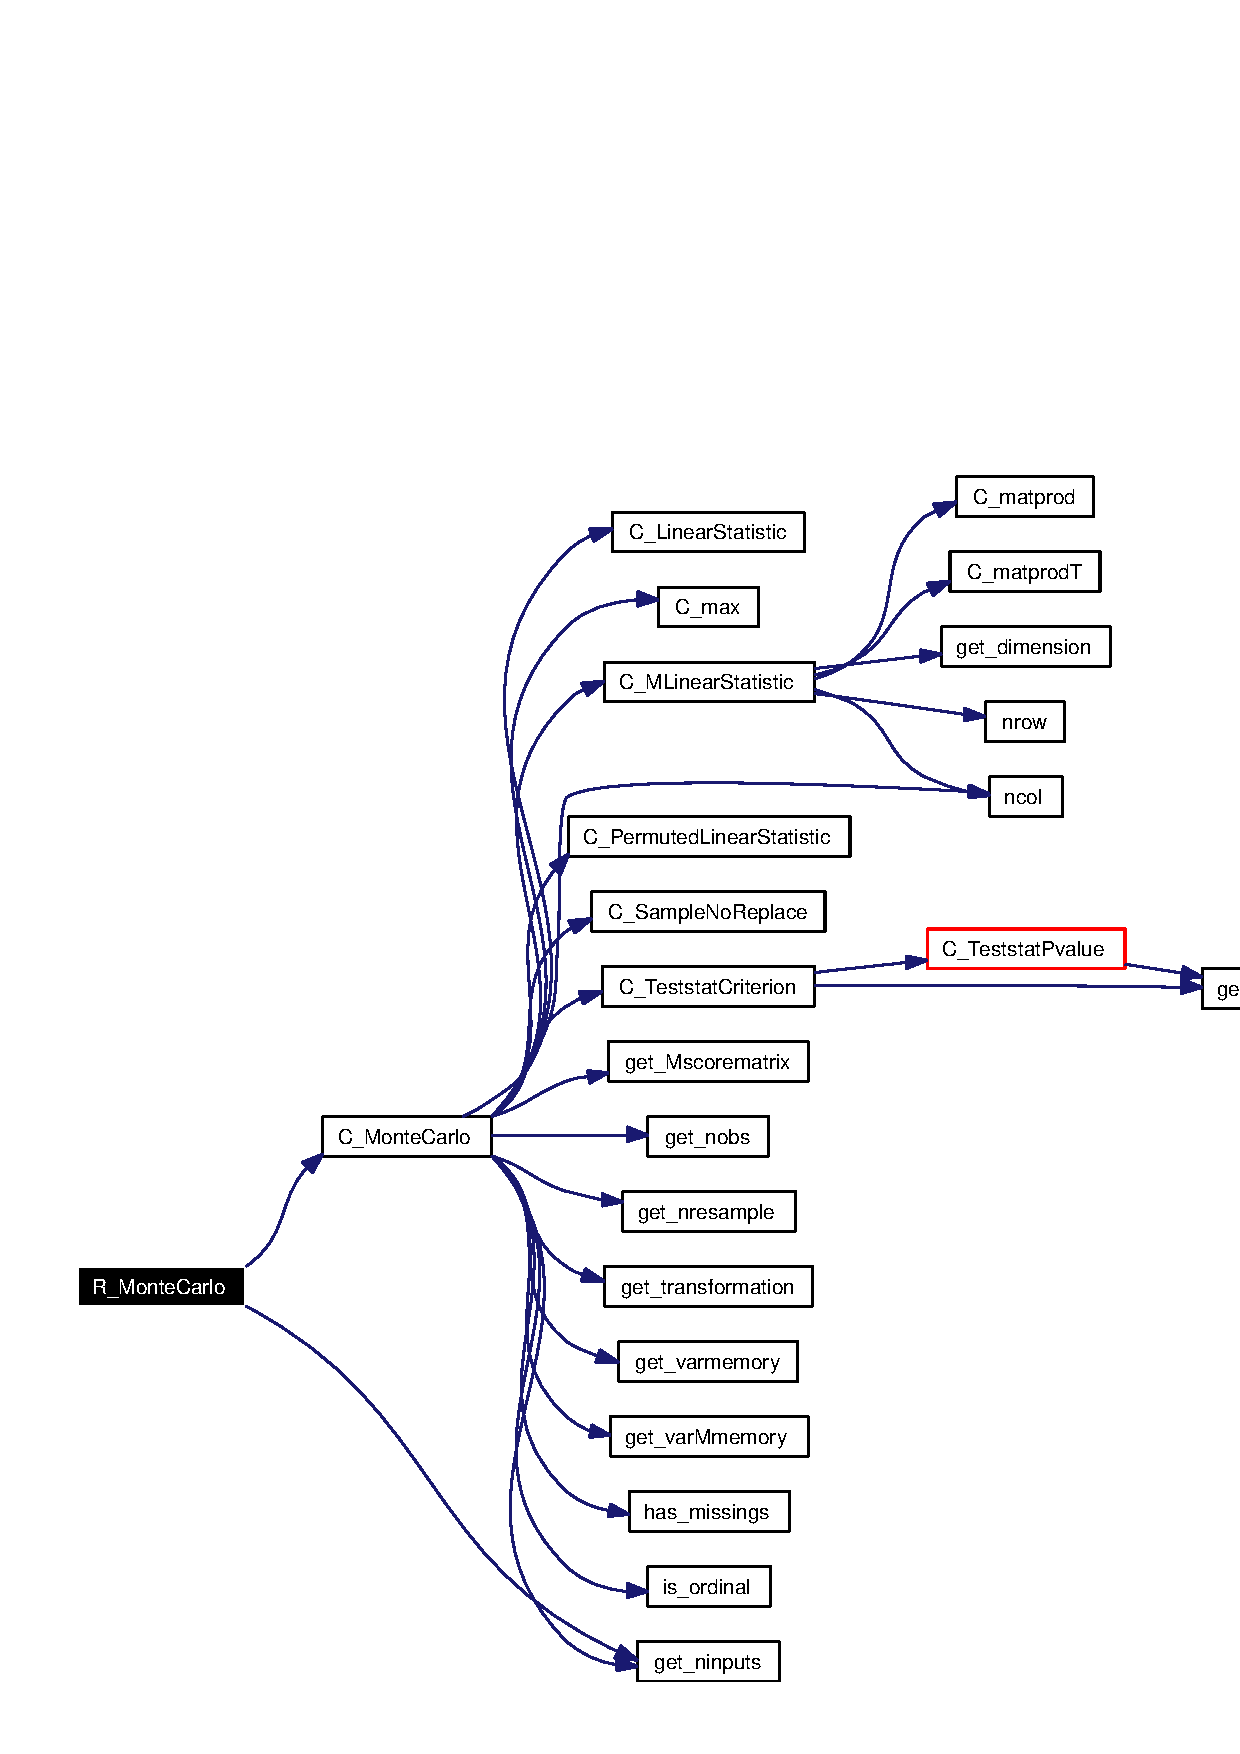
\includegraphics[width=321pt]{Distributions_8c_a5_cgraph}
\end{center}
\end{figure}
\hypertarget{Distributions_8c_a1}{
\index{Distributions.c@{Distributions.c}!R_quadformConditionalPvalue@{R\_\-quadformConditionalPvalue}}
\index{R_quadformConditionalPvalue@{R\_\-quadformConditionalPvalue}!Distributions.c@{Distributions.c}}
\subsubsection[R\_\-quadformConditionalPvalue]{\setlength{\rightskip}{0pt plus 5cm}SEXP R\_\-quadform\-Conditional\-Pvalue (SEXP {\em tstat}, SEXP {\em df})}}
\label{Distributions_8c_a1}


R-interface to C\_\-quadform\-Conditional\-Pvalue\par
 \begin{Desc}
\item[Parameters:]
\begin{description}
\item[{\em tstat}]test statitstic \item[{\em df}]degree of freedom \end{description}
\end{Desc}


Definition at line 29 of file Distributions.c.

References C\_\-quadform\-Conditional\-Pvalue().

Here is the call graph for this function:\begin{figure}[H]
\begin{center}
\leavevmode
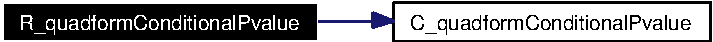
\includegraphics[width=188pt]{Distributions_8c_a1_cgraph}
\end{center}
\end{figure}

\hypertarget{Distributions_8h}{
\section{Distributions.h File Reference}
\label{Distributions_8h}\index{Distributions.h@{Distributions.h}}
}


This graph shows which files directly or indirectly include this file:\begin{figure}[H]
\begin{center}
\leavevmode
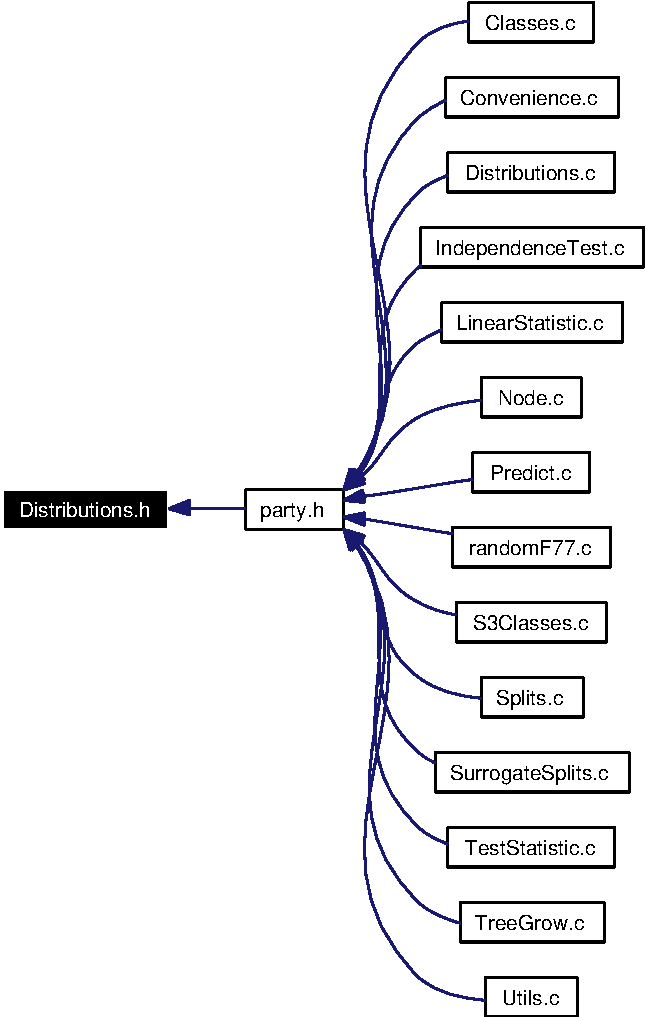
\includegraphics[width=172pt]{Distributions_8h__dep__incl}
\end{center}
\end{figure}
\subsection*{Functions}
\begin{CompactItemize}
\item 
double \hyperlink{Distributions_8h_a692392488ab88e95a62d2142e9d428c}{C\_\-quadform\-Conditional\-Pvalue} (const double tstat, const double df)
\item 
double \hyperlink{Distributions_8h_0b0373aa22dcf8b8ecf6b9c560db9c70}{C\_\-maxabs\-Conditional\-Pvalue} (const double tstat, const double $\ast$Sigma, const int pq, int $\ast$maxpts, double $\ast$releps, double $\ast$abseps, double $\ast$tol)
\item 
void \hyperlink{Distributions_8h_579a9b99cc4ab820a62f636869788cf8}{C\_\-Monte\-Carlo} (double $\ast$pvalues, SEXP learnsample, SEXP weights, SEXP fitmem, SEXP varctrl, SEXP gtctrl, double $\ast$ans)
\end{CompactItemize}


\subsection{Function Documentation}
\hypertarget{Distributions_8h_0b0373aa22dcf8b8ecf6b9c560db9c70}{
\index{Distributions.h@{Distributions.h}!C_maxabsConditionalPvalue@{C\_\-maxabsConditionalPvalue}}
\index{C_maxabsConditionalPvalue@{C\_\-maxabsConditionalPvalue}!Distributions.h@{Distributions.h}}
\subsubsection[C\_\-maxabsConditionalPvalue]{\setlength{\rightskip}{0pt plus 5cm}double C\_\-maxabs\-Conditional\-Pvalue (const double {\em tstat}, const double $\ast$ {\em Sigma}, const int {\em pq}, int $\ast$ {\em maxpts}, double $\ast$ {\em releps}, double $\ast$ {\em abseps}, double $\ast$ {\em tol})}}
\label{Distributions_8h_0b0373aa22dcf8b8ecf6b9c560db9c70}


Conditional asymptotic P-value of a maxabs-type test statistic\par
 Basically the functionality from package `mvtnorm' \par
 \begin{Desc}
\item[Parameters:]
\begin{description}
\item[{\em tstat}]test statitstic \item[{\em Sigma}]covariance matrix \item[{\em pq}]nrow(Sigma) \item[{\em maxpts}]number of Monte-Carlo steps \item[{\em releps}]relative error \item[{\em abseps}]absolute error \item[{\em tol}]tolerance \end{description}
\end{Desc}


Definition at line 52 of file Distributions.c.

Referenced by C\_\-Conditional\-Pvalue(), and R\_\-maxabs\-Conditional\-Pvalue().\hypertarget{Distributions_8h_579a9b99cc4ab820a62f636869788cf8}{
\index{Distributions.h@{Distributions.h}!C_MonteCarlo@{C\_\-MonteCarlo}}
\index{C_MonteCarlo@{C\_\-MonteCarlo}!Distributions.h@{Distributions.h}}
\subsubsection[C\_\-MonteCarlo]{\setlength{\rightskip}{0pt plus 5cm}void C\_\-Monte\-Carlo (double $\ast$ {\em criterion}, SEXP {\em learnsample}, SEXP {\em weights}, SEXP {\em fitmem}, SEXP {\em varctrl}, SEXP {\em gtctrl}, double $\ast$ {\em ans\_\-pvalues})}}
\label{Distributions_8h_579a9b99cc4ab820a62f636869788cf8}


Monte-Carlo approximation to the conditional pvalues \begin{Desc}
\item[Parameters:]
\begin{description}
\item[{\em criterion}]vector of node criteria for each input \item[{\em learnsample}]an object of class `Learning\-Sample' \item[{\em weights}]case weights \item[{\em fitmem}]an object of class `Tree\-Fit\-Memory' \item[{\em varctrl}]an object of class `Variable\-Control' \item[{\em gtctrl}]an object of class `Global\-Test\-Control' \item[{\em ans\_\-pvalues}]return values; vector of adjusted pvalues \end{description}
\end{Desc}


Definition at line 169 of file Distributions.c.

References get\_\-jointtransf(), get\_\-ninputs(), get\_\-nobs(), get\_\-nresample(), PL2\_\-expcovinf\-Sym, PL2\_\-inputs\-Sym, PL2\_\-responses\-Sym, and PL2\_\-sumweights\-Sym.

Referenced by R\_\-Monte\-Carlo().

Here is the call graph for this function:\begin{figure}[H]
\begin{center}
\leavevmode
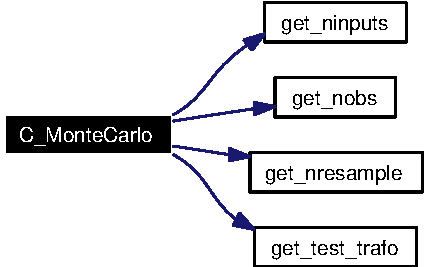
\includegraphics[width=119pt]{Distributions_8h_579a9b99cc4ab820a62f636869788cf8_cgraph}
\end{center}
\end{figure}
\hypertarget{Distributions_8h_a692392488ab88e95a62d2142e9d428c}{
\index{Distributions.h@{Distributions.h}!C_quadformConditionalPvalue@{C\_\-quadformConditionalPvalue}}
\index{C_quadformConditionalPvalue@{C\_\-quadformConditionalPvalue}!Distributions.h@{Distributions.h}}
\subsubsection[C\_\-quadformConditionalPvalue]{\setlength{\rightskip}{0pt plus 5cm}double C\_\-quadform\-Conditional\-Pvalue (const double {\em tstat}, const double {\em df})}}
\label{Distributions_8h_a692392488ab88e95a62d2142e9d428c}


Conditional asymptotic P-value of a quadratic form\par
 \begin{Desc}
\item[Parameters:]
\begin{description}
\item[{\em tstat}]test statistic \item[{\em df}]degree of freedom \end{description}
\end{Desc}


Definition at line 18 of file Distributions.c.

Referenced by C\_\-Conditional\-Pvalue(), and R\_\-quadform\-Conditional\-Pvalue().
\hypertarget{IndependenceTest_8c}{
\section{IndependenceTest.c File Reference}
\label{IndependenceTest_8c}\index{IndependenceTest.c@{IndependenceTest.c}}
}
{\tt \#include \char`\"{}party.h\char`\"{}}\par


Include dependency graph for IndependenceTest.c:\nopagebreak
\begin{figure}[H]
\begin{center}
\leavevmode
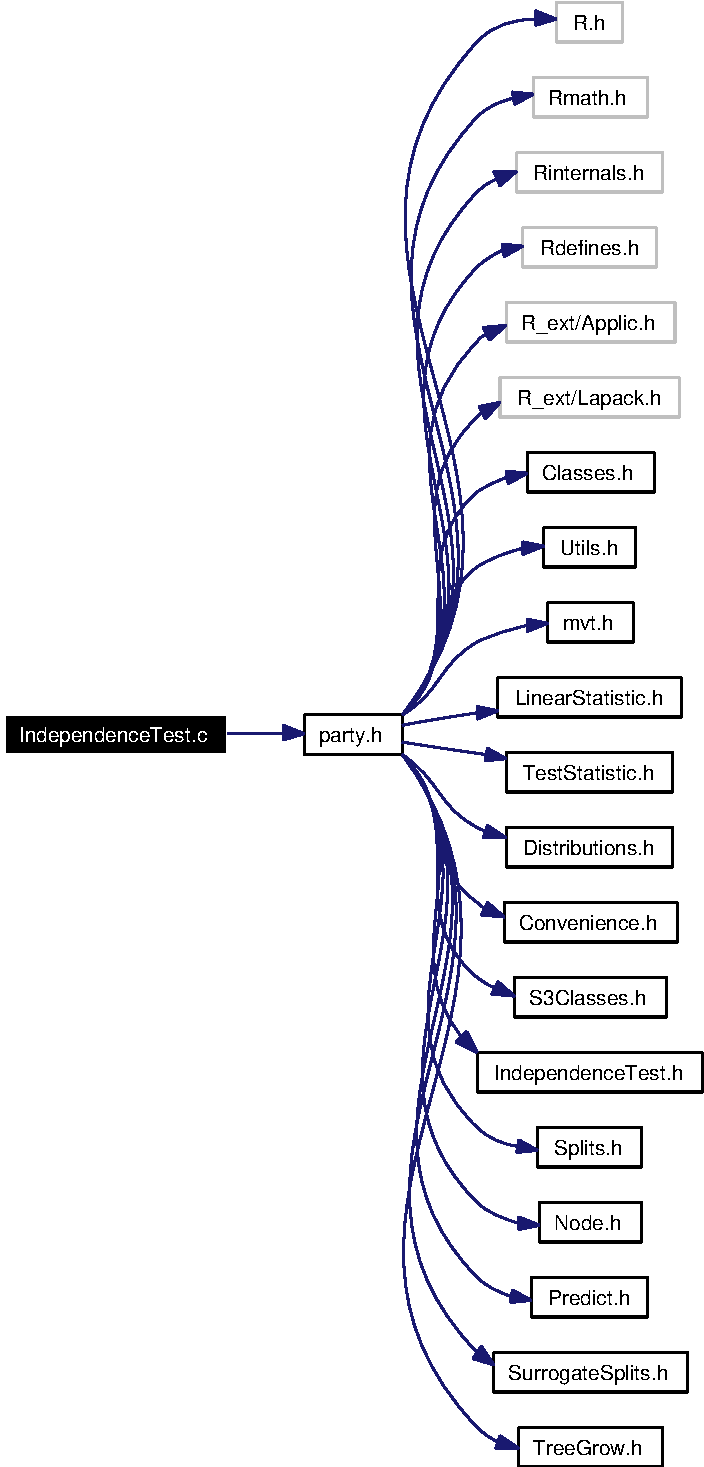
\includegraphics[width=420pt]{IndependenceTest_8c__incl}
\end{center}
\end{figure}
\subsection*{Functions}
\begin{CompactItemize}
\item 
void \hyperlink{IndependenceTest_8c_b02275a67ad210d96fed9864590ee3ef}{C\_\-TeststatPvalue} (const SEXP linexpcov, const SEXP varctrl, double $\ast$ans\_\-teststat, double $\ast$ans\_\-pvalue)
\item 
void \hyperlink{IndependenceTest_8c_d33688ffc38df769a95d6964e5bb193a}{C\_\-TeststatCriterion} (const SEXP linexpcov, const SEXP varctrl, double $\ast$ans\_\-teststat, double $\ast$ans\_\-criterion)
\item 
void \hyperlink{IndependenceTest_8c_e64c8d91a58113cee43788dc1663d645}{C\_\-IndependenceTest} (const SEXP x, const SEXP y, const SEXP weights, SEXP linexpcov, SEXP varctrl, SEXP ans)
\item 
SEXP \hyperlink{IndependenceTest_8c_aab8e2db15687b6b95f802dd1719ed54}{R\_\-IndependenceTest} (SEXP x, SEXP y, SEXP weights, SEXP linexpcov, SEXP varctrl)
\item 
void \hyperlink{IndependenceTest_8c_0de2357bd1d38058c0cfc68c3e743b34}{C\_\-GlobalTest} (const SEXP learnsample, const SEXP weights, SEXP fitmem, const SEXP varctrl, const SEXP gtctrl, const double minsplit, double $\ast$ans\_\-teststat, double $\ast$ans\_\-criterion)
\item 
SEXP \hyperlink{IndependenceTest_8c_f80dcff3dd9196b9f861fd83f4efa8ac}{R\_\-GlobalTest} (SEXP learnsample, SEXP weights, SEXP fitmem, SEXP varctrl, SEXP gtctrl)
\end{CompactItemize}


\subsection{Detailed Description}
Functions for variable selection in each node of a tree

\begin{Desc}
\item[Author:]\begin{Desc}
\item[Author]\end{Desc}
\end{Desc}
\begin{Desc}
\item[Date:]\begin{Desc}
\item[Date]\end{Desc}
\end{Desc}


Definition in file \hyperlink{IndependenceTest_8c-source}{IndependenceTest.c}.

\subsection{Function Documentation}
\hypertarget{IndependenceTest_8c_0de2357bd1d38058c0cfc68c3e743b34}{
\index{IndependenceTest.c@{IndependenceTest.c}!C_GlobalTest@{C\_\-GlobalTest}}
\index{C_GlobalTest@{C\_\-GlobalTest}!IndependenceTest.c@{IndependenceTest.c}}
\subsubsection{\setlength{\rightskip}{0pt plus 5cm}void C\_\-GlobalTest (const SEXP {\em learnsample}, const SEXP {\em weights}, SEXP {\em fitmem}, const SEXP {\em varctrl}, const SEXP {\em gtctrl}, const double {\em minsplit}, double $\ast$ {\em ans\_\-teststat}, double $\ast$ {\em ans\_\-criterion})}}
\label{IndependenceTest_8c_0de2357bd1d38058c0cfc68c3e743b34}


Perform a global test on independence of a response and multiple inputs \par
 \begin{Desc}
\item[Parameters:]
\begin{description}
\item[{\em learnsample}]an object of class `LearningSample' \item[{\em weights}]case weights \item[{\em fitmem}]an object of class `TreeFitMemory' \item[{\em varctrl}]an object of class `VariableControl' \item[{\em gtctrl}]an object of class `GlobalTestControl' \item[{\em minsplit}]minimum sum of weights to proceed \item[{\em ans\_\-teststat}]return value; vector of test statistics \item[{\em ans\_\-criterion}]return value; vector of node criteria (adjusted) pvalues or raw test statistics \end{description}
\end{Desc}


Definition at line 129 of file IndependenceTest.c.

Referenced by C\_\-Node(), and R\_\-GlobalTest().\hypertarget{IndependenceTest_8c_e64c8d91a58113cee43788dc1663d645}{
\index{IndependenceTest.c@{IndependenceTest.c}!C_IndependenceTest@{C\_\-IndependenceTest}}
\index{C_IndependenceTest@{C\_\-IndependenceTest}!IndependenceTest.c@{IndependenceTest.c}}
\subsubsection{\setlength{\rightskip}{0pt plus 5cm}void C\_\-IndependenceTest (const SEXP {\em x}, const SEXP {\em y}, const SEXP {\em weights}, SEXP {\em linexpcov}, SEXP {\em varctrl}, SEXP {\em ans})}}
\label{IndependenceTest_8c_e64c8d91a58113cee43788dc1663d645}


Test of independence between x and y \par
 \begin{Desc}
\item[Parameters:]
\begin{description}
\item[{\em x}]values of the transformation \item[{\em y}]values of the influence function \item[{\em weights}]case weights \item[{\em linexpcov}]an object of class `VariableControl' for T \item[{\em varctrl}]an object of class `VariableControl' \item[{\em ans;}]return value, a double vector (teststat, pvalue) \end{description}
\end{Desc}


Definition at line 78 of file IndependenceTest.c.

References C\_\-LinStatExpCov(), C\_\-LinStatExpCovMPinv(), C\_\-TeststatPvalue(), get\_\-teststat(), get\_\-tol(), ncol(), nrow(), and PL2\_\-expcovinfSym.

Referenced by R\_\-IndependenceTest().

Here is the call graph for this function:\nopagebreak
\begin{figure}[H]
\begin{center}
\leavevmode
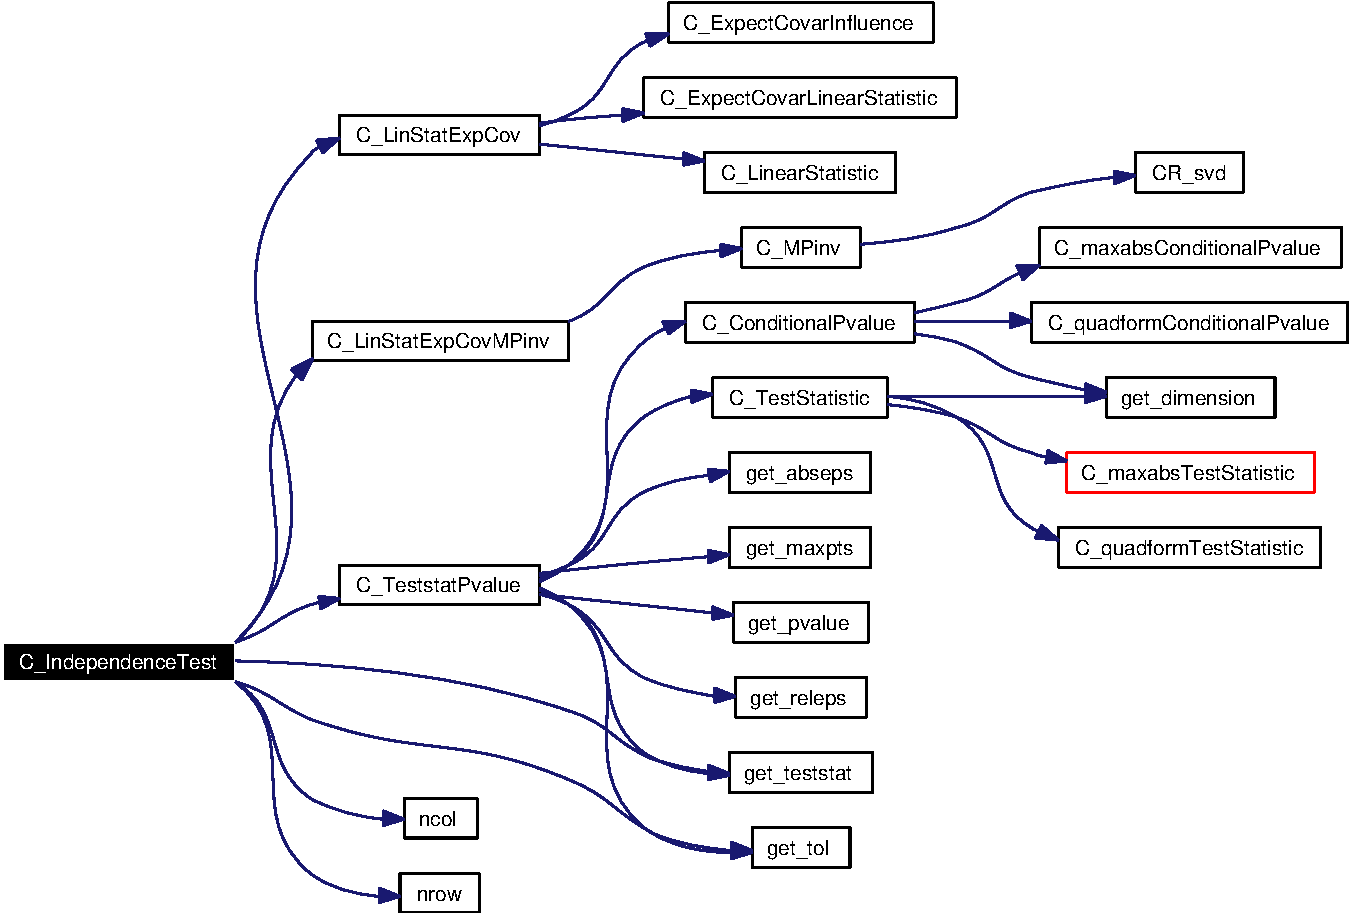
\includegraphics[width=165pt]{IndependenceTest_8c_e64c8d91a58113cee43788dc1663d645_cgraph}
\end{center}
\end{figure}
\hypertarget{IndependenceTest_8c_d33688ffc38df769a95d6964e5bb193a}{
\index{IndependenceTest.c@{IndependenceTest.c}!C_TeststatCriterion@{C\_\-TeststatCriterion}}
\index{C_TeststatCriterion@{C\_\-TeststatCriterion}!IndependenceTest.c@{IndependenceTest.c}}
\subsubsection{\setlength{\rightskip}{0pt plus 5cm}void C\_\-TeststatCriterion (const SEXP {\em linexpcov}, const SEXP {\em varctrl}, double $\ast$ {\em ans\_\-teststat}, double $\ast$ {\em ans\_\-criterion})}}
\label{IndependenceTest_8c_d33688ffc38df769a95d6964e5bb193a}


Computes the test statistic and the node criterion \par
 \begin{Desc}
\item[Parameters:]
\begin{description}
\item[{\em linexpcov}]an object of class `LinStatExpectCovar' \item[{\em varctrl}]an object of class `VariableControl' \item[{\em ans\_\-teststat;}]return value, the test statistic \item[{\em ans\_\-criterion;}]return value, thep-value \end{description}
\end{Desc}


Definition at line 53 of file IndependenceTest.c.

Referenced by C\_\-GlobalTest(), and C\_\-MonteCarlo().\hypertarget{IndependenceTest_8c_b02275a67ad210d96fed9864590ee3ef}{
\index{IndependenceTest.c@{IndependenceTest.c}!C_TeststatPvalue@{C\_\-TeststatPvalue}}
\index{C_TeststatPvalue@{C\_\-TeststatPvalue}!IndependenceTest.c@{IndependenceTest.c}}
\subsubsection{\setlength{\rightskip}{0pt plus 5cm}void C\_\-TeststatPvalue (const SEXP {\em linexpcov}, const SEXP {\em varctrl}, double $\ast$ {\em ans\_\-teststat}, double $\ast$ {\em ans\_\-pvalue})}}
\label{IndependenceTest_8c_b02275a67ad210d96fed9864590ee3ef}


Computes the test statistic and, if requested, the corresponding P-value for a linear statistic \par
 \begin{Desc}
\item[Parameters:]
\begin{description}
\item[{\em linexpcov}]an object of class `LinStatExpectCovar' \item[{\em varctrl}]an object of class `VariableControl' \item[{\em ans\_\-teststat;}]return value, the test statistic \item[{\em ans\_\-pvalue;}]return value, the p-value \end{description}
\end{Desc}


Definition at line 21 of file IndependenceTest.c.

Referenced by C\_\-IndependenceTest(), and C\_\-TeststatCriterion().\hypertarget{IndependenceTest_8c_f80dcff3dd9196b9f861fd83f4efa8ac}{
\index{IndependenceTest.c@{IndependenceTest.c}!R_GlobalTest@{R\_\-GlobalTest}}
\index{R_GlobalTest@{R\_\-GlobalTest}!IndependenceTest.c@{IndependenceTest.c}}
\subsubsection{\setlength{\rightskip}{0pt plus 5cm}SEXP R\_\-GlobalTest (SEXP {\em learnsample}, SEXP {\em weights}, SEXP {\em fitmem}, SEXP {\em varctrl}, SEXP {\em gtctrl})}}
\label{IndependenceTest_8c_f80dcff3dd9196b9f861fd83f4efa8ac}


R-interface to C\_\-GlobalTest \par
 \begin{Desc}
\item[Parameters:]
\begin{description}
\item[{\em learnsample}]an object of class `LearningSample' \item[{\em weights}]case weights \item[{\em fitmem}]an object of class `TreeFitMemory' \item[{\em varctrl}]an object of class `VariableControl' \item[{\em gtctrl}]an object of class `GlobalTestControl' \end{description}
\end{Desc}


Definition at line 272 of file IndependenceTest.c.

References C\_\-GlobalTest(), and get\_\-ninputs().

Here is the call graph for this function:\nopagebreak
\begin{figure}[H]
\begin{center}
\leavevmode
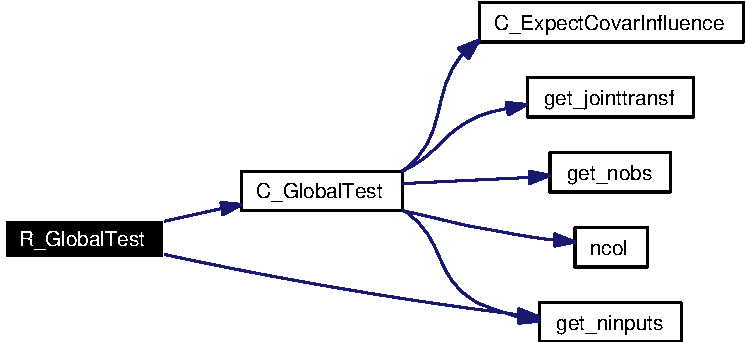
\includegraphics[width=117pt]{IndependenceTest_8c_f80dcff3dd9196b9f861fd83f4efa8ac_cgraph}
\end{center}
\end{figure}
\hypertarget{IndependenceTest_8c_aab8e2db15687b6b95f802dd1719ed54}{
\index{IndependenceTest.c@{IndependenceTest.c}!R_IndependenceTest@{R\_\-IndependenceTest}}
\index{R_IndependenceTest@{R\_\-IndependenceTest}!IndependenceTest.c@{IndependenceTest.c}}
\subsubsection{\setlength{\rightskip}{0pt plus 5cm}SEXP R\_\-IndependenceTest (SEXP {\em x}, SEXP {\em y}, SEXP {\em weights}, SEXP {\em linexpcov}, SEXP {\em varctrl})}}
\label{IndependenceTest_8c_aab8e2db15687b6b95f802dd1719ed54}


R-interface to C\_\-IndependenceTest \par
 \begin{Desc}
\item[Parameters:]
\begin{description}
\item[{\em x}]values of the transformation \item[{\em y}]values of the influence function \item[{\em weights}]case weights \item[{\em linexpcov}]an object of class `VariableControl' for T \item[{\em varctrl}]an object of class `VariableControl' \end{description}
\end{Desc}


Definition at line 105 of file IndependenceTest.c.

References C\_\-IndependenceTest().

Here is the call graph for this function:\nopagebreak
\begin{figure}[H]
\begin{center}
\leavevmode
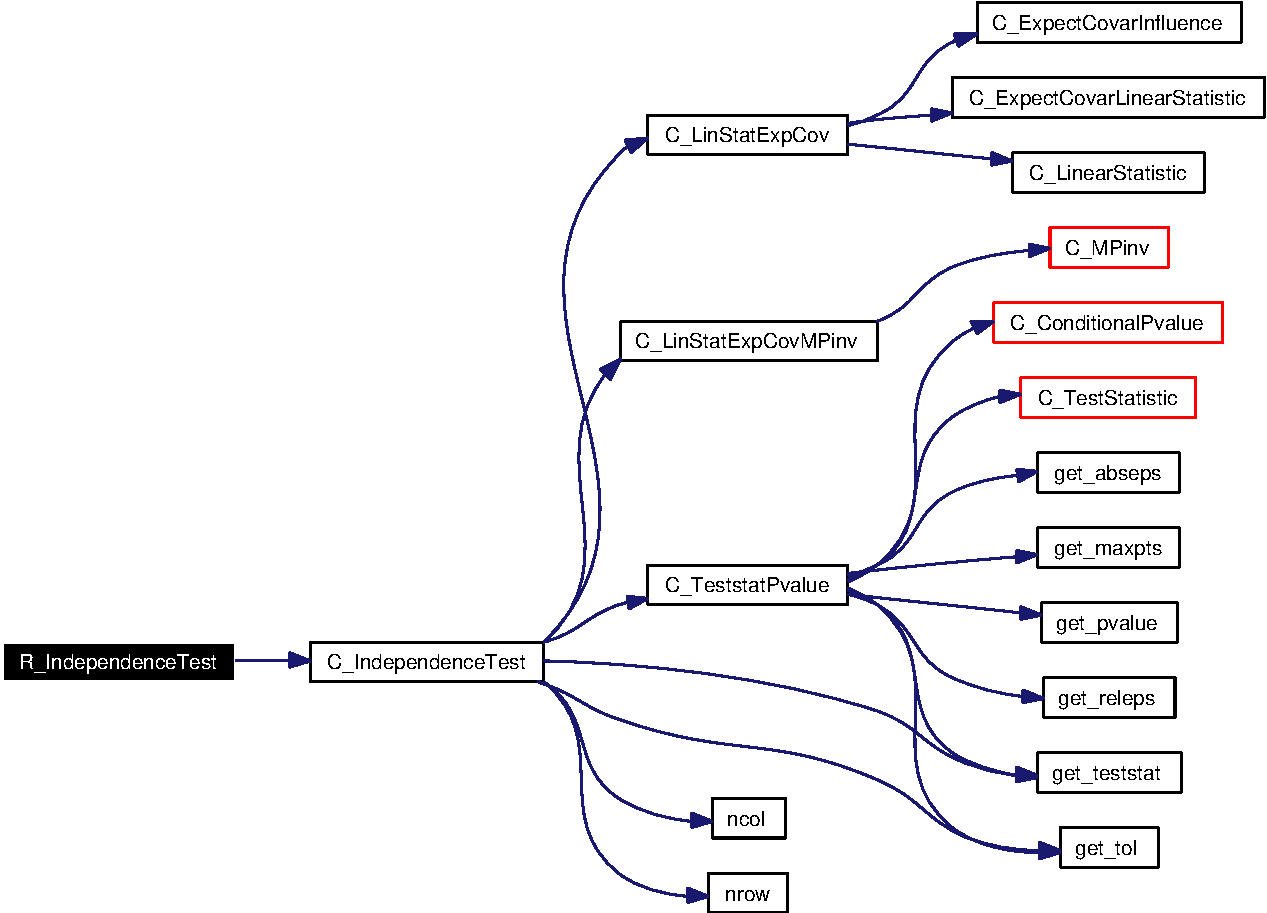
\includegraphics[width=240pt]{IndependenceTest_8c_aab8e2db15687b6b95f802dd1719ed54_cgraph}
\end{center}
\end{figure}

\hypertarget{IndependenceTest_8h}{
\section{IndependenceTest.h File Reference}
\label{IndependenceTest_8h}\index{IndependenceTest.h@{IndependenceTest.h}}
}


This graph shows which files directly or indirectly include this file:\nopagebreak
\begin{figure}[H]
\begin{center}
\leavevmode
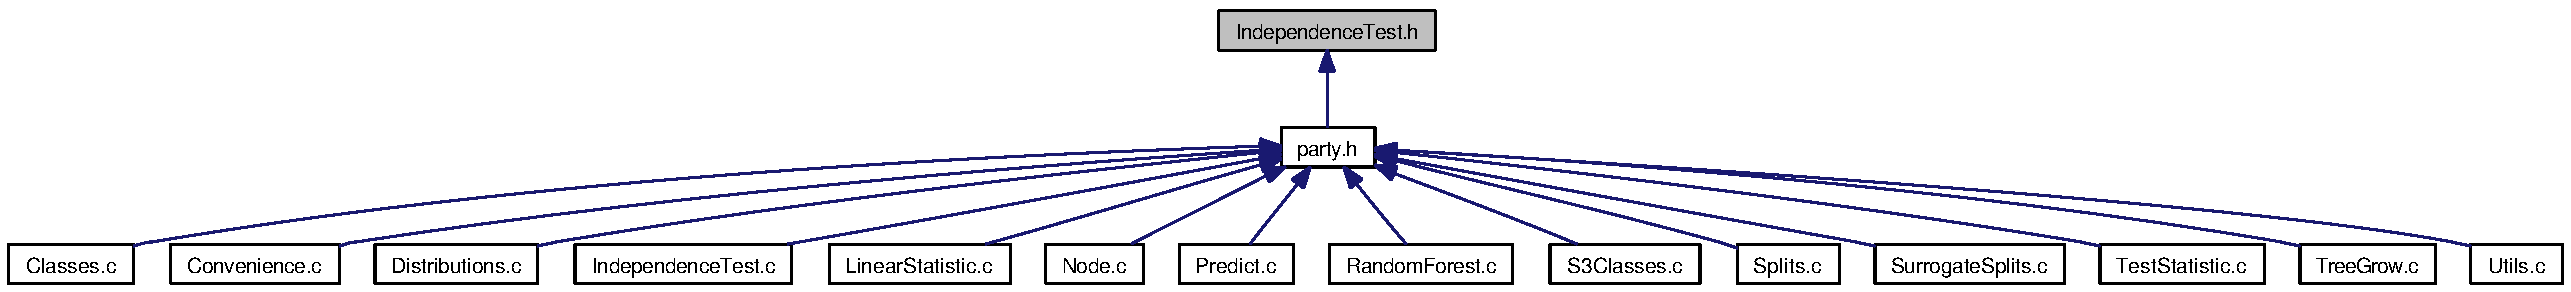
\includegraphics[width=420pt]{IndependenceTest_8h__dep__incl}
\end{center}
\end{figure}
\subsection*{Functions}
\begin{CompactItemize}
\item 
void \hyperlink{IndependenceTest_8h_cef73c662621fad56562bfc743025cc5}{C\_\-GlobalTest} (SEXP learnsample, SEXP weights, SEXP fitmem, SEXP varctrl, SEXP gtestctrl, double minsplit, double $\ast$teststat, double $\ast$criterion)
\item 
void \hyperlink{IndependenceTest_8h_b02275a67ad210d96fed9864590ee3ef}{C\_\-TeststatPvalue} (const SEXP linexpcov, const SEXP varctrl, double $\ast$ans\_\-teststat, double $\ast$ans\_\-pvalue)
\item 
void \hyperlink{IndependenceTest_8h_d33688ffc38df769a95d6964e5bb193a}{C\_\-TeststatCriterion} (const SEXP linexpcov, const SEXP varctrl, double $\ast$ans\_\-teststat, double $\ast$ans\_\-criterion)
\end{CompactItemize}


\subsection{Function Documentation}
\hypertarget{IndependenceTest_8h_cef73c662621fad56562bfc743025cc5}{
\index{IndependenceTest.h@{IndependenceTest.h}!C\_\-GlobalTest@{C\_\-GlobalTest}}
\index{C\_\-GlobalTest@{C\_\-GlobalTest}!IndependenceTest.h@{IndependenceTest.h}}
\subsubsection[C\_\-GlobalTest]{\setlength{\rightskip}{0pt plus 5cm}void C\_\-GlobalTest (const SEXP {\em learnsample}, \/  const SEXP {\em weights}, \/  SEXP {\em fitmem}, \/  const SEXP {\em varctrl}, \/  const SEXP {\em gtctrl}, \/  const double {\em minsplit}, \/  double $\ast$ {\em ans\_\-teststat}, \/  double $\ast$ {\em ans\_\-criterion})}}
\label{IndependenceTest_8h_cef73c662621fad56562bfc743025cc5}


Perform a global test on independence of a response and multiple inputs \par
 \begin{Desc}
\item[Parameters:]
\begin{description}
\item[{\em learnsample}]an object of class `LearningSample' \item[{\em weights}]case weights \item[{\em fitmem}]an object of class `TreeFitMemory' \item[{\em varctrl}]an object of class `VariableControl' \item[{\em gtctrl}]an object of class `GlobalTestControl' \item[{\em minsplit}]minimum sum of weights to proceed \item[{\em ans\_\-teststat}]return value; vector of test statistics \item[{\em ans\_\-criterion}]return value; vector of node criteria (adjusted) pvalues or raw test statistics \end{description}
\end{Desc}


Definition at line 129 of file IndependenceTest.c.

References AGGREGATED, BONFERRONI, C\_\-ExpectCovarInfluence(), C\_\-LinStatExpCov(), C\_\-LinStatExpCovMPinv(), C\_\-MonteCarlo(), C\_\-SampleNoReplace(), C\_\-tempweights(), C\_\-TeststatCriterion(), get\_\-dontuse(), get\_\-dontusetmp(), get\_\-mtry(), get\_\-ninputs(), get\_\-nobs(), get\_\-randomsplits(), get\_\-test\_\-trafo(), get\_\-teststat(), get\_\-testtype(), get\_\-tol(), get\_\-transformation(), get\_\-varmemory(), has\_\-missings(), MONTECARLO, ncol(), nrow(), PL2\_\-expcovinfSym, PL2\_\-inputsSym, PL2\_\-responsesSym, PL2\_\-sumweightsSym, TESTSTATISTIC, and UNIVARIATE.

Referenced by C\_\-Node(), and R\_\-GlobalTest().

Here is the call graph for this function:\nopagebreak
\begin{figure}[H]
\begin{center}
\leavevmode
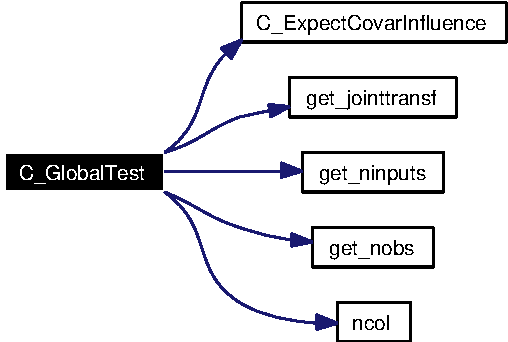
\includegraphics[width=420pt]{IndependenceTest_8h_cef73c662621fad56562bfc743025cc5_cgraph}
\end{center}
\end{figure}
\hypertarget{IndependenceTest_8h_d33688ffc38df769a95d6964e5bb193a}{
\index{IndependenceTest.h@{IndependenceTest.h}!C\_\-TeststatCriterion@{C\_\-TeststatCriterion}}
\index{C\_\-TeststatCriterion@{C\_\-TeststatCriterion}!IndependenceTest.h@{IndependenceTest.h}}
\subsubsection[C\_\-TeststatCriterion]{\setlength{\rightskip}{0pt plus 5cm}void C\_\-TeststatCriterion (const SEXP {\em linexpcov}, \/  const SEXP {\em varctrl}, \/  double $\ast$ {\em ans\_\-teststat}, \/  double $\ast$ {\em ans\_\-criterion})}}
\label{IndependenceTest_8h_d33688ffc38df769a95d6964e5bb193a}


Computes the test statistic and the node criterion \par
 \begin{Desc}
\item[Parameters:]
\begin{description}
\item[{\em linexpcov}]an object of class `LinStatExpectCovar' \item[{\em varctrl}]an object of class `VariableControl' \item[{\em ans\_\-teststat;}]return value, the test statistic \item[{\em ans\_\-criterion;}]return value, thep-value \end{description}
\end{Desc}


Definition at line 53 of file IndependenceTest.c.

References C\_\-TeststatPvalue(), and get\_\-pvalue().

Referenced by C\_\-GlobalTest(), and C\_\-MonteCarlo().

Here is the call graph for this function:\nopagebreak
\begin{figure}[H]
\begin{center}
\leavevmode
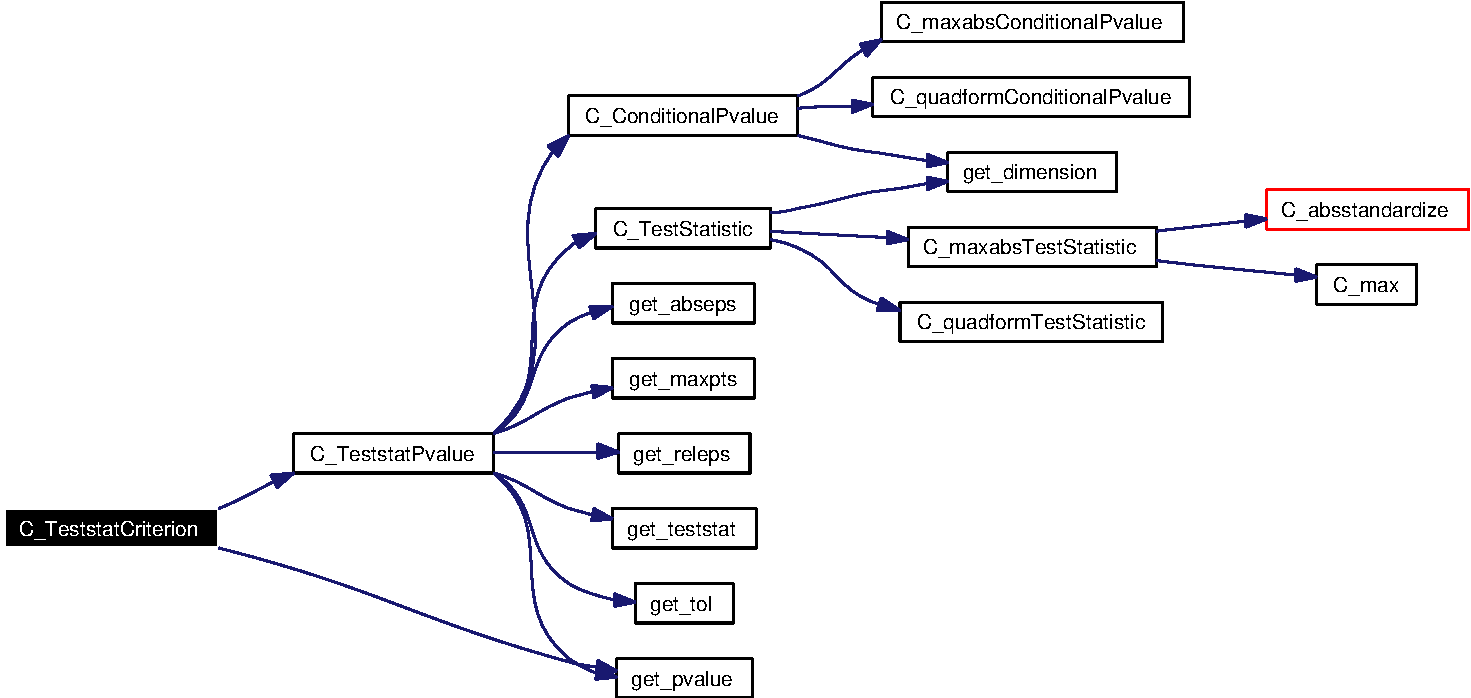
\includegraphics[width=420pt]{IndependenceTest_8h_d33688ffc38df769a95d6964e5bb193a_cgraph}
\end{center}
\end{figure}
\hypertarget{IndependenceTest_8h_b02275a67ad210d96fed9864590ee3ef}{
\index{IndependenceTest.h@{IndependenceTest.h}!C\_\-TeststatPvalue@{C\_\-TeststatPvalue}}
\index{C\_\-TeststatPvalue@{C\_\-TeststatPvalue}!IndependenceTest.h@{IndependenceTest.h}}
\subsubsection[C\_\-TeststatPvalue]{\setlength{\rightskip}{0pt plus 5cm}void C\_\-TeststatPvalue (const SEXP {\em linexpcov}, \/  const SEXP {\em varctrl}, \/  double $\ast$ {\em ans\_\-teststat}, \/  double $\ast$ {\em ans\_\-pvalue})}}
\label{IndependenceTest_8h_b02275a67ad210d96fed9864590ee3ef}


Computes the test statistic and, if requested, the corresponding P-value for a linear statistic \par
 \begin{Desc}
\item[Parameters:]
\begin{description}
\item[{\em linexpcov}]an object of class `LinStatExpectCovar' \item[{\em varctrl}]an object of class `VariableControl' \item[{\em ans\_\-teststat;}]return value, the test statistic \item[{\em ans\_\-pvalue;}]return value, the p-value \end{description}
\end{Desc}


Definition at line 21 of file IndependenceTest.c.

References C\_\-ConditionalPvalue(), C\_\-TestStatistic(), get\_\-abseps(), get\_\-maxpts(), get\_\-pvalue(), get\_\-releps(), get\_\-teststat(), and get\_\-tol().

Referenced by C\_\-IndependenceTest(), and C\_\-TeststatCriterion().

Here is the call graph for this function:\nopagebreak
\begin{figure}[H]
\begin{center}
\leavevmode
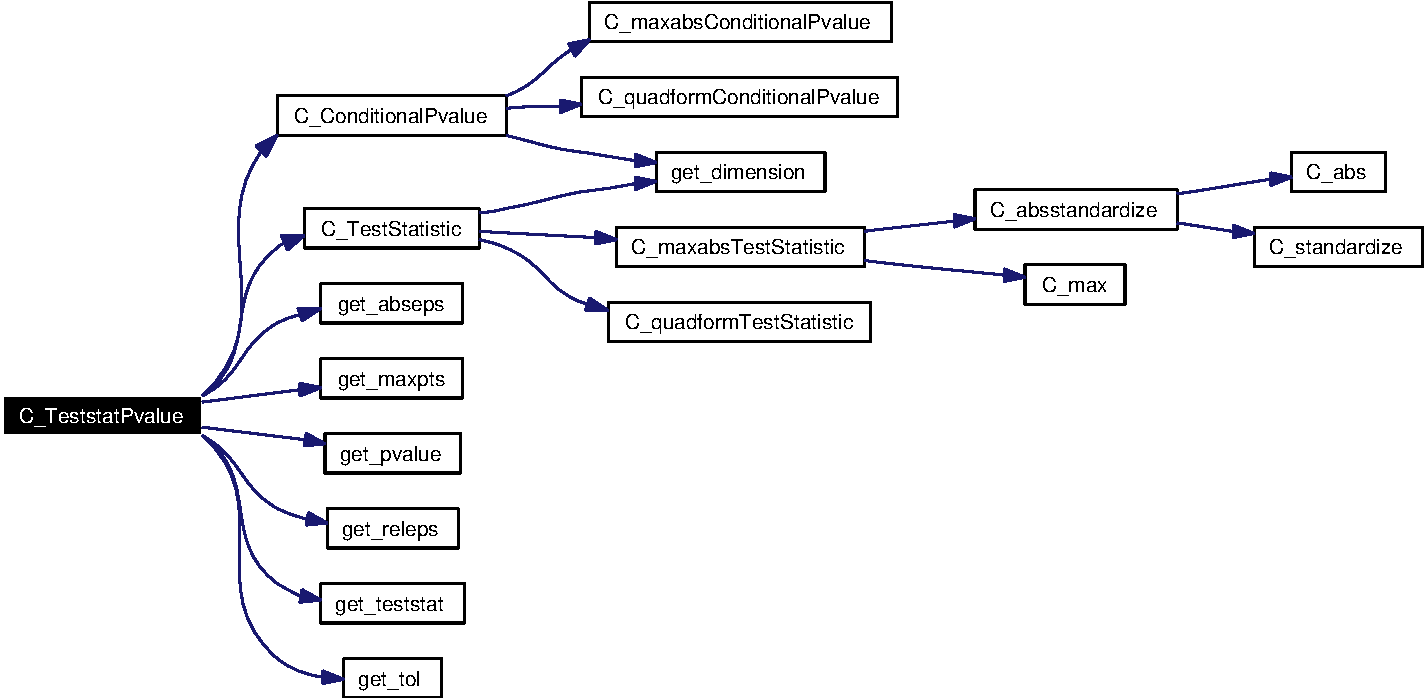
\includegraphics[width=354pt]{IndependenceTest_8h_b02275a67ad210d96fed9864590ee3ef_cgraph}
\end{center}
\end{figure}

\hypertarget{LinearStatistic_8c}{
\section{LinearStatistic.c File Reference}
\label{LinearStatistic_8c}\index{LinearStatistic.c@{LinearStatistic.c}}
}
{\tt \#include \char`\"{}party.h\char`\"{}}\par


Include dependency graph for LinearStatistic.c:\nopagebreak
\begin{figure}[H]
\begin{center}
\leavevmode
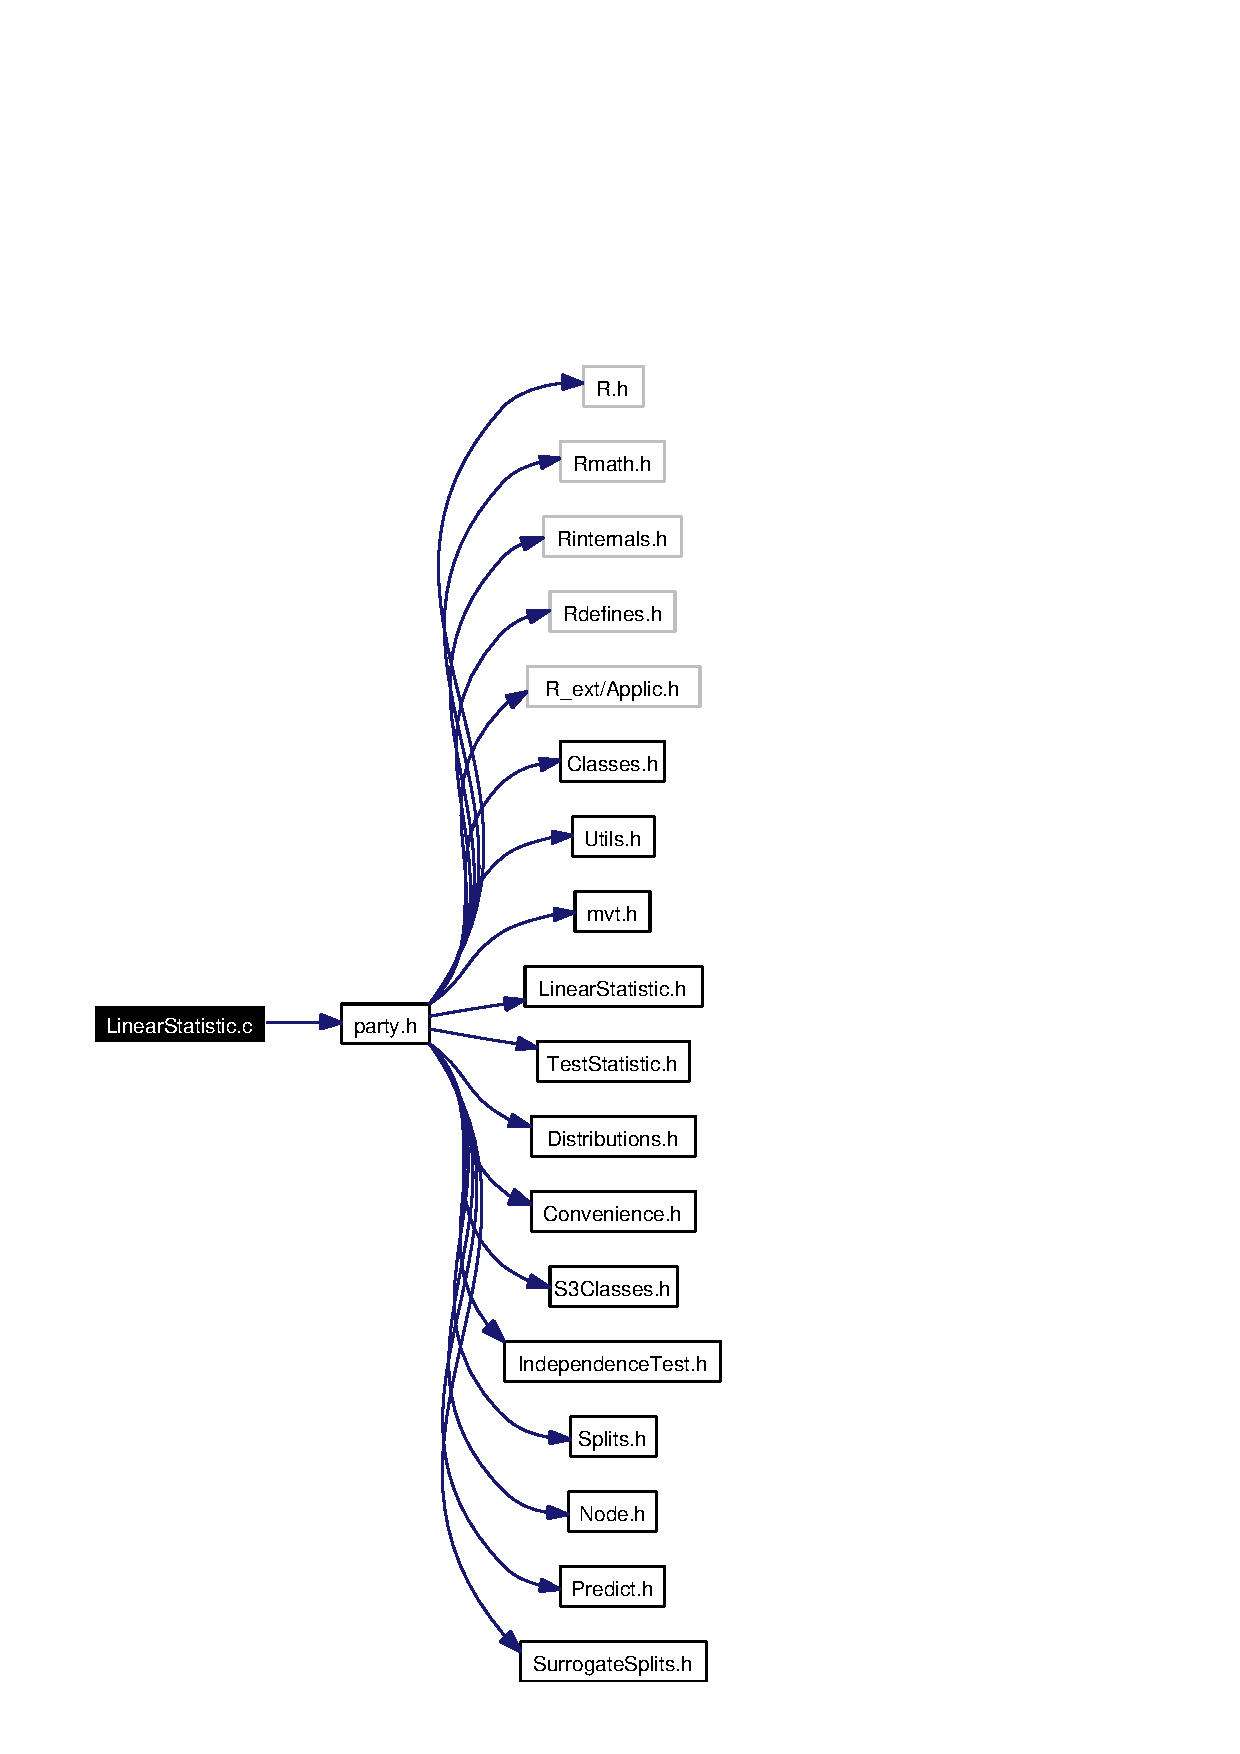
\includegraphics[width=420pt]{LinearStatistic_8c__incl}
\end{center}
\end{figure}
\subsection*{Functions}
\begin{CompactItemize}
\item 
void \hyperlink{LinearStatistic_8c_aefa2a9406bb30b323715e3db41da637}{C\_\-LinearStatistic} (const double $\ast$x, const int p, const double $\ast$y, const int q, const double $\ast$weights, const int n, double $\ast$ans)
\item 
SEXP \hyperlink{LinearStatistic_8c_732bfc8e1797d8953482aa31f9b43e5f}{R\_\-LinearStatistic} (SEXP x, SEXP y, SEXP weights)
\item 
void \hyperlink{LinearStatistic_8c_e2f62abe13ee5b625141b5d4a496d832}{C\_\-ExpectCovarInfluence} (const double $\ast$y, const int q, const double $\ast$weights, const int n, SEXP ans)
\item 
SEXP \hyperlink{LinearStatistic_8c_6216ea560644c08002fb32756ae67dcc}{R\_\-ExpectCovarInfluence} (SEXP y, SEXP weights)
\item 
void \hyperlink{LinearStatistic_8c_94a0805ea258af79d426c095feee399a}{C\_\-ExpectCovarLinearStatistic} (const double $\ast$x, const int p, const double $\ast$y, const int q, const double $\ast$weights, const int n, const SEXP expcovinf, SEXP ans)
\item 
SEXP \hyperlink{LinearStatistic_8c_58fff8082d3ab197994a21a10c422353}{R\_\-ExpectCovarLinearStatistic} (SEXP x, SEXP y, SEXP weights, SEXP expcovinf)
\item 
void \hyperlink{LinearStatistic_8c_a34b0f12fac36231a105d6dc903bfe89}{C\_\-PermutedLinearStatistic} (const double $\ast$x, const int p, const double $\ast$y, const int q, const int n, const int nperm, const int $\ast$indx, const int $\ast$perm, double $\ast$ans)
\item 
SEXP \hyperlink{LinearStatistic_8c_be383bcae17e8b3a1d5740ec16a9817a}{R\_\-PermutedLinearStatistic} (SEXP x, SEXP y, SEXP indx, SEXP perm)
\end{CompactItemize}


\subsection{Detailed Description}
Linear statistics for conditional inference based on Strasser \& Weber (1999)

\begin{Desc}
\item[Author:]\begin{Desc}
\item[Author]\end{Desc}
\end{Desc}
\begin{Desc}
\item[Date:]\begin{Desc}
\item[Date]\end{Desc}
\end{Desc}


Definition in file \hyperlink{LinearStatistic_8c-source}{LinearStatistic.c}.

\subsection{Function Documentation}
\hypertarget{LinearStatistic_8c_e2f62abe13ee5b625141b5d4a496d832}{
\index{LinearStatistic.c@{LinearStatistic.c}!C_ExpectCovarInfluence@{C\_\-ExpectCovarInfluence}}
\index{C_ExpectCovarInfluence@{C\_\-ExpectCovarInfluence}!LinearStatistic.c@{LinearStatistic.c}}
\subsubsection{\setlength{\rightskip}{0pt plus 5cm}void C\_\-ExpectCovarInfluence (const double $\ast$ {\em y}, const int {\em q}, const double $\ast$ {\em weights}, const int {\em n}, SEXP {\em ans})}}
\label{LinearStatistic_8c_e2f62abe13ee5b625141b5d4a496d832}


Conditional expectation and covariance of the influence function\par
 \begin{Desc}
\item[Parameters:]
\begin{description}
\item[{\em y}]values of the influence function \item[{\em q}]dimension of the influence function \item[{\em weights}]case weights \item[{\em n}]number of observations \item[{\em ans}]return value; an object of class `ExpectCovarInfluence' \end{description}
\end{Desc}


Definition at line 101 of file LinearStatistic.c.

Referenced by C\_\-GlobalTest(), C\_\-LinStatExpCov(), C\_\-surrogates(), and R\_\-ExpectCovarInfluence().\hypertarget{LinearStatistic_8c_94a0805ea258af79d426c095feee399a}{
\index{LinearStatistic.c@{LinearStatistic.c}!C_ExpectCovarLinearStatistic@{C\_\-ExpectCovarLinearStatistic}}
\index{C_ExpectCovarLinearStatistic@{C\_\-ExpectCovarLinearStatistic}!LinearStatistic.c@{LinearStatistic.c}}
\subsubsection{\setlength{\rightskip}{0pt plus 5cm}void C\_\-ExpectCovarLinearStatistic (const double $\ast$ {\em x}, const int {\em p}, const double $\ast$ {\em y}, const int {\em q}, const double $\ast$ {\em weights}, const int {\em n}, const SEXP {\em expcovinf}, SEXP {\em ans})}}
\label{LinearStatistic_8c_94a0805ea258af79d426c095feee399a}


Conditional expectation and covariance of the a linear statistic\par
 \begin{Desc}
\item[Parameters:]
\begin{description}
\item[{\em x}]values of the transformation \item[{\em p}]dimension of the transformation \item[{\em y}]values of the influence function \item[{\em q}]dimension of the influence function \item[{\em weights}]case weights \item[{\em n}]number of observations \item[{\em expcovinf}]an object of class `ExpectCovarInfluence' \item[{\em ans}]return value; an object of class `ExpectCovar' \end{description}
\end{Desc}


Definition at line 213 of file LinearStatistic.c.

Referenced by C\_\-LinStatExpCov(), and R\_\-ExpectCovarLinearStatistic().\hypertarget{LinearStatistic_8c_aefa2a9406bb30b323715e3db41da637}{
\index{LinearStatistic.c@{LinearStatistic.c}!C_LinearStatistic@{C\_\-LinearStatistic}}
\index{C_LinearStatistic@{C\_\-LinearStatistic}!LinearStatistic.c@{LinearStatistic.c}}
\subsubsection{\setlength{\rightskip}{0pt plus 5cm}void C\_\-LinearStatistic (const double $\ast$ {\em x}, const int {\em p}, const double $\ast$ {\em y}, const int {\em q}, const double $\ast$ {\em weights}, const int {\em n}, double $\ast$ {\em ans})}}
\label{LinearStatistic_8c_aefa2a9406bb30b323715e3db41da637}


Computes the linear statistic, formula (1) in the paper\par
 \begin{Desc}
\item[Parameters:]
\begin{description}
\item[{\em x}]values of the transformation \item[{\em p}]dimension of the transformation \item[{\em y}]values of the influence function \item[{\em q}]dimension of the influence function \item[{\em weights}]case weights \item[{\em n}]number of observations \item[{\em ans}]return value; a pointer to a REALSXP-vector of length pq \end{description}
\end{Desc}


Definition at line 23 of file LinearStatistic.c.

Referenced by C\_\-LinStatExpCov(), C\_\-MonteCarlo(), and R\_\-LinearStatistic().\hypertarget{LinearStatistic_8c_a34b0f12fac36231a105d6dc903bfe89}{
\index{LinearStatistic.c@{LinearStatistic.c}!C_PermutedLinearStatistic@{C\_\-PermutedLinearStatistic}}
\index{C_PermutedLinearStatistic@{C\_\-PermutedLinearStatistic}!LinearStatistic.c@{LinearStatistic.c}}
\subsubsection{\setlength{\rightskip}{0pt plus 5cm}void C\_\-PermutedLinearStatistic (const double $\ast$ {\em x}, const int {\em p}, const double $\ast$ {\em y}, const int {\em q}, const int {\em n}, const int {\em nperm}, const int $\ast$ {\em indx}, const int $\ast$ {\em perm}, double $\ast$ {\em ans})}}
\label{LinearStatistic_8c_a34b0f12fac36231a105d6dc903bfe89}


Linear Statistic with permuted indices\par
 \begin{Desc}
\item[Parameters:]
\begin{description}
\item[{\em x}]values of the transformation \item[{\em p}]dimension of the transformation \item[{\em y}]values of the influence function \item[{\em q}]dimension of the influence function \item[{\em n}]number of observations \item[{\em nperm}]number of permutations \item[{\em indx}]indices for the x-part \item[{\em perm}](permuted) indices for the y-part \item[{\em ans}]return value; a pointer to a REALSXP-vector of length pq \end{description}
\end{Desc}


Definition at line 351 of file LinearStatistic.c.

Referenced by C\_\-MonteCarlo(), and R\_\-PermutedLinearStatistic().\hypertarget{LinearStatistic_8c_6216ea560644c08002fb32756ae67dcc}{
\index{LinearStatistic.c@{LinearStatistic.c}!R_ExpectCovarInfluence@{R\_\-ExpectCovarInfluence}}
\index{R_ExpectCovarInfluence@{R\_\-ExpectCovarInfluence}!LinearStatistic.c@{LinearStatistic.c}}
\subsubsection{\setlength{\rightskip}{0pt plus 5cm}SEXP R\_\-ExpectCovarInfluence (SEXP {\em y}, SEXP {\em weights})}}
\label{LinearStatistic_8c_6216ea560644c08002fb32756ae67dcc}


R-interface to C\_\-ExpectCovarInfluence\par
 \begin{Desc}
\item[Parameters:]
\begin{description}
\item[{\em y}]values of the influence function \item[{\em weights}]case weights \end{description}
\end{Desc}


Definition at line 171 of file LinearStatistic.c.\hypertarget{LinearStatistic_8c_58fff8082d3ab197994a21a10c422353}{
\index{LinearStatistic.c@{LinearStatistic.c}!R_ExpectCovarLinearStatistic@{R\_\-ExpectCovarLinearStatistic}}
\index{R_ExpectCovarLinearStatistic@{R\_\-ExpectCovarLinearStatistic}!LinearStatistic.c@{LinearStatistic.c}}
\subsubsection{\setlength{\rightskip}{0pt plus 5cm}SEXP R\_\-ExpectCovarLinearStatistic (SEXP {\em x}, SEXP {\em y}, SEXP {\em weights}, SEXP {\em expcovinf})}}
\label{LinearStatistic_8c_58fff8082d3ab197994a21a10c422353}


R-interface to C\_\-ExpectCovarLinearStatistic\par
 \begin{Desc}
\item[Parameters:]
\begin{description}
\item[{\em x}]values of the transformation \item[{\em y}]values of the influence function \item[{\em weights}]case weights \item[{\em expcovinf}]an object of class `ExpectCovarInfluence' \end{description}
\end{Desc}


Definition at line 306 of file LinearStatistic.c.

References C\_\-ExpectCovarLinearStatistic(), ncol(), nrow(), PL2\_\-covarianceSym, and PL2\_\-expectationSym.

Here is the call graph for this function:\nopagebreak
\begin{figure}[H]
\begin{center}
\leavevmode
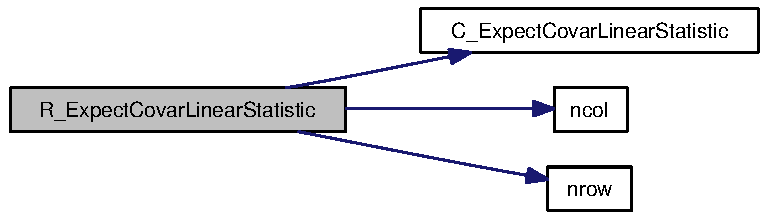
\includegraphics[width=202pt]{LinearStatistic_8c_58fff8082d3ab197994a21a10c422353_cgraph}
\end{center}
\end{figure}
\hypertarget{LinearStatistic_8c_732bfc8e1797d8953482aa31f9b43e5f}{
\index{LinearStatistic.c@{LinearStatistic.c}!R_LinearStatistic@{R\_\-LinearStatistic}}
\index{R_LinearStatistic@{R\_\-LinearStatistic}!LinearStatistic.c@{LinearStatistic.c}}
\subsubsection{\setlength{\rightskip}{0pt plus 5cm}SEXP R\_\-LinearStatistic (SEXP {\em x}, SEXP {\em y}, SEXP {\em weights})}}
\label{LinearStatistic_8c_732bfc8e1797d8953482aa31f9b43e5f}


R-interface to C\_\-LinearStatistic \par
 \begin{Desc}
\item[Parameters:]
\begin{description}
\item[{\em x}]values of the transformation \item[{\em y}]values of the influence function \item[{\em weights}]case weights \end{description}
\end{Desc}


Definition at line 59 of file LinearStatistic.c.

References C\_\-LinearStatistic(), ncol(), and nrow().

Here is the call graph for this function:\nopagebreak
\begin{figure}[H]
\begin{center}
\leavevmode
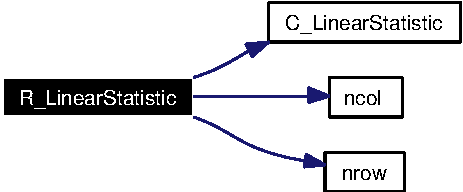
\includegraphics[width=138pt]{LinearStatistic_8c_732bfc8e1797d8953482aa31f9b43e5f_cgraph}
\end{center}
\end{figure}
\hypertarget{LinearStatistic_8c_be383bcae17e8b3a1d5740ec16a9817a}{
\index{LinearStatistic.c@{LinearStatistic.c}!R_PermutedLinearStatistic@{R\_\-PermutedLinearStatistic}}
\index{R_PermutedLinearStatistic@{R\_\-PermutedLinearStatistic}!LinearStatistic.c@{LinearStatistic.c}}
\subsubsection{\setlength{\rightskip}{0pt plus 5cm}SEXP R\_\-PermutedLinearStatistic (SEXP {\em x}, SEXP {\em y}, SEXP {\em indx}, SEXP {\em perm})}}
\label{LinearStatistic_8c_be383bcae17e8b3a1d5740ec16a9817a}


Linear Statistic with permuted indices\par
 \begin{Desc}
\item[Parameters:]
\begin{description}
\item[{\em x}]values of the transformation \item[{\em y}]values of the influence function \item[{\em indx}]indices for the x-part \item[{\em perm}](permuted) indices for the y-part \end{description}
\end{Desc}


Definition at line 384 of file LinearStatistic.c.

References C\_\-PermutedLinearStatistic(), ncol(), and nrow().

Here is the call graph for this function:\nopagebreak
\begin{figure}[H]
\begin{center}
\leavevmode

\includegraphics[width=187pt]{LinearStatistic_8c_be383bcae17e8b3a1d5740ec16a9817a_cgraph}
\end{center}
\end{figure}

\hypertarget{LinearStatistic_8h}{
\section{Linear\-Statistic.h File Reference}
\label{LinearStatistic_8h}\index{LinearStatistic.h@{LinearStatistic.h}}
}


This graph shows which files directly or indirectly include this file:\begin{figure}[H]
\begin{center}
\leavevmode
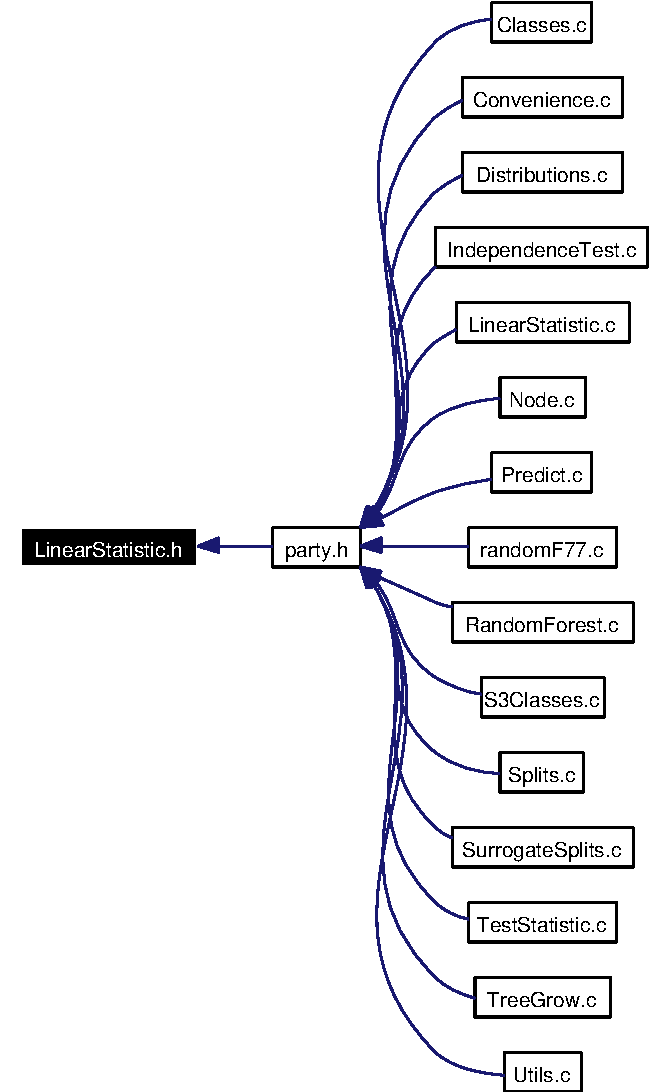
\includegraphics[width=177pt]{LinearStatistic_8h__dep__incl}
\end{center}
\end{figure}
\subsection*{Functions}
\begin{CompactItemize}
\item 
void \hyperlink{LinearStatistic_8h_a0}{C\_\-Linear\-Statistic} (const double $\ast$x, const int p, const double $\ast$y, const int q, const double $\ast$weights, const int n, double $\ast$ans)
\item 
void \hyperlink{LinearStatistic_8h_a1}{C\_\-Expect\-Covar\-Influence} (const double $\ast$y, const int q, const double $\ast$weights, const int n, SEXP ans)
\item 
void \hyperlink{LinearStatistic_8h_a2}{C\_\-Expect\-Covar\-Linear\-Statistic} (const double $\ast$x, const int p, const double $\ast$y, const int q, const double $\ast$weights, const int n, const SEXP expcovinf, SEXP ans)
\item 
void \hyperlink{LinearStatistic_8h_a3}{C\_\-Permuted\-Linear\-Statistic} (const double $\ast$x, const int p, const double $\ast$y, const int q, const int n, const int nperm, const int $\ast$indx, const int $\ast$perm, double $\ast$ans)
\item 
SEXP \hyperlink{LinearStatistic_8h_a4}{R\_\-Expect\-Covar\-Influence} (SEXP y, SEXP weights)
\end{CompactItemize}


\subsection{Function Documentation}
\hypertarget{LinearStatistic_8h_a1}{
\index{LinearStatistic.h@{Linear\-Statistic.h}!C_ExpectCovarInfluence@{C\_\-ExpectCovarInfluence}}
\index{C_ExpectCovarInfluence@{C\_\-ExpectCovarInfluence}!LinearStatistic.h@{Linear\-Statistic.h}}
\subsubsection[C\_\-ExpectCovarInfluence]{\setlength{\rightskip}{0pt plus 5cm}void C\_\-Expect\-Covar\-Influence (const double $\ast$ {\em y}, const int {\em q}, const double $\ast$ {\em weights}, const int {\em n}, SEXP {\em ans})}}
\label{LinearStatistic_8h_a1}


Conditional expectation and covariance of the influence function\par
 \begin{Desc}
\item[Parameters:]
\begin{description}
\item[{\em y}]values of the influence function \item[{\em q}]dimension of the influence function \item[{\em weights}]case weights \item[{\em n}]number of observations \item[{\em ans}]return value; an object of class `Expect\-Covar\-Influence' \end{description}
\end{Desc}


Definition at line 101 of file Linear\-Statistic.c.

References PL2\_\-covariance\-Sym, PL2\_\-expectation\-Sym, and PL2\_\-sumweights\-Sym.

Referenced by C\_\-Global\-Test(), C\_\-Lin\-Stat\-Exp\-Cov(), C\_\-surrogates(), and R\_\-Expect\-Covar\-Influence().\hypertarget{LinearStatistic_8h_a2}{
\index{LinearStatistic.h@{Linear\-Statistic.h}!C_ExpectCovarLinearStatistic@{C\_\-ExpectCovarLinearStatistic}}
\index{C_ExpectCovarLinearStatistic@{C\_\-ExpectCovarLinearStatistic}!LinearStatistic.h@{Linear\-Statistic.h}}
\subsubsection[C\_\-ExpectCovarLinearStatistic]{\setlength{\rightskip}{0pt plus 5cm}void C\_\-Expect\-Covar\-Linear\-Statistic (const double $\ast$ {\em x}, const int {\em p}, const double $\ast$ {\em y}, const int {\em q}, const double $\ast$ {\em weights}, const int {\em n}, const SEXP {\em expcovinf}, SEXP {\em ans})}}
\label{LinearStatistic_8h_a2}


Conditional expectation and covariance of the a linear statistic\par
 \begin{Desc}
\item[Parameters:]
\begin{description}
\item[{\em x}]values of the transformation \item[{\em p}]dimension of the transformation \item[{\em y}]values of the influence function \item[{\em q}]dimension of the influence function \item[{\em weights}]case weights \item[{\em n}]number of observations \item[{\em expcovinf}]an object of class `Expect\-Covar\-Influence' \item[{\em ans}]return value; an object of class `Expect\-Covar' \end{description}
\end{Desc}


Definition at line 213 of file Linear\-Statistic.c.

References C\_\-kronecker(), PL2\_\-covariance\-Sym, PL2\_\-expectation\-Sym, and PL2\_\-sumweights\-Sym.

Referenced by C\_\-Lin\-Stat\-Exp\-Cov(), and R\_\-Expect\-Covar\-Linear\-Statistic().

Here is the call graph for this function:\begin{figure}[H]
\begin{center}
\leavevmode
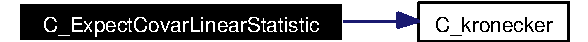
\includegraphics[width=158pt]{LinearStatistic_8h_a2_cgraph}
\end{center}
\end{figure}
\hypertarget{LinearStatistic_8h_a0}{
\index{LinearStatistic.h@{Linear\-Statistic.h}!C_LinearStatistic@{C\_\-LinearStatistic}}
\index{C_LinearStatistic@{C\_\-LinearStatistic}!LinearStatistic.h@{Linear\-Statistic.h}}
\subsubsection[C\_\-LinearStatistic]{\setlength{\rightskip}{0pt plus 5cm}void C\_\-Linear\-Statistic (const double $\ast$ {\em x}, const int {\em p}, const double $\ast$ {\em y}, const int {\em q}, const double $\ast$ {\em weights}, const int {\em n}, double $\ast$ {\em ans})}}
\label{LinearStatistic_8h_a0}


Computes the linear statistic, formula (1) in the paper\par
 \begin{Desc}
\item[Parameters:]
\begin{description}
\item[{\em x}]values of the transformation \item[{\em p}]dimension of the transformation \item[{\em y}]values of the influence function \item[{\em q}]dimension of the influence function \item[{\em weights}]case weights \item[{\em n}]number of observations \item[{\em ans}]return value; a pointer to a REALSXP-vector of length pq \end{description}
\end{Desc}


Definition at line 23 of file Linear\-Statistic.c.

Referenced by C\_\-Lin\-Stat\-Exp\-Cov(), C\_\-Monte\-Carlo(), and R\_\-Linear\-Statistic().\hypertarget{LinearStatistic_8h_a3}{
\index{LinearStatistic.h@{Linear\-Statistic.h}!C_PermutedLinearStatistic@{C\_\-PermutedLinearStatistic}}
\index{C_PermutedLinearStatistic@{C\_\-PermutedLinearStatistic}!LinearStatistic.h@{Linear\-Statistic.h}}
\subsubsection[C\_\-PermutedLinearStatistic]{\setlength{\rightskip}{0pt plus 5cm}void C\_\-Permuted\-Linear\-Statistic (const double $\ast$ {\em x}, const int {\em p}, const double $\ast$ {\em y}, const int {\em q}, const int {\em n}, const int {\em nperm}, const int $\ast$ {\em indx}, const int $\ast$ {\em perm}, double $\ast$ {\em ans})}}
\label{LinearStatistic_8h_a3}


Linear Statistic with permuted indices\par
 \begin{Desc}
\item[Parameters:]
\begin{description}
\item[{\em x}]values of the transformation \item[{\em p}]dimension of the transformation \item[{\em y}]values of the influence function \item[{\em q}]dimension of the influence function \item[{\em n}]number of observations \item[{\em nperm}]number of permutations \item[{\em indx}]indices for the x-part \item[{\em perm}](permuted) indices for the y-part \item[{\em ans}]return value; a pointer to a REALSXP-vector of length pq \end{description}
\end{Desc}


Definition at line 351 of file Linear\-Statistic.c.

Referenced by C\_\-Monte\-Carlo(), and R\_\-Permuted\-Linear\-Statistic().\hypertarget{LinearStatistic_8h_a4}{
\index{LinearStatistic.h@{Linear\-Statistic.h}!R_ExpectCovarInfluence@{R\_\-ExpectCovarInfluence}}
\index{R_ExpectCovarInfluence@{R\_\-ExpectCovarInfluence}!LinearStatistic.h@{Linear\-Statistic.h}}
\subsubsection[R\_\-ExpectCovarInfluence]{\setlength{\rightskip}{0pt plus 5cm}SEXP R\_\-Expect\-Covar\-Influence (SEXP {\em y}, SEXP {\em weights})}}
\label{LinearStatistic_8h_a4}


R-interface to C\_\-Expect\-Covar\-Influence\par
 \begin{Desc}
\item[Parameters:]
\begin{description}
\item[{\em y}]values of the influence function \item[{\em weights}]case weights \end{description}
\end{Desc}


Definition at line 171 of file Linear\-Statistic.c.

References C\_\-Expect\-Covar\-Influence(), ncol(), nrow(), PL2\_\-covariance\-Sym, PL2\_\-expectation\-Sym, and PL2\_\-sumweights\-Sym.

Here is the call graph for this function:\begin{figure}[H]
\begin{center}
\leavevmode
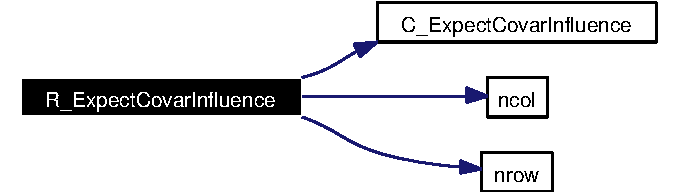
\includegraphics[width=179pt]{LinearStatistic_8h_a4_cgraph}
\end{center}
\end{figure}

\hypertarget{mvt_8h}{
\section{mvt.h File Reference}
\label{mvt_8h}\index{mvt.h@{mvt.h}}
}


This graph shows which files directly or indirectly include this file:\nopagebreak
\begin{figure}[H]
\begin{center}
\leavevmode
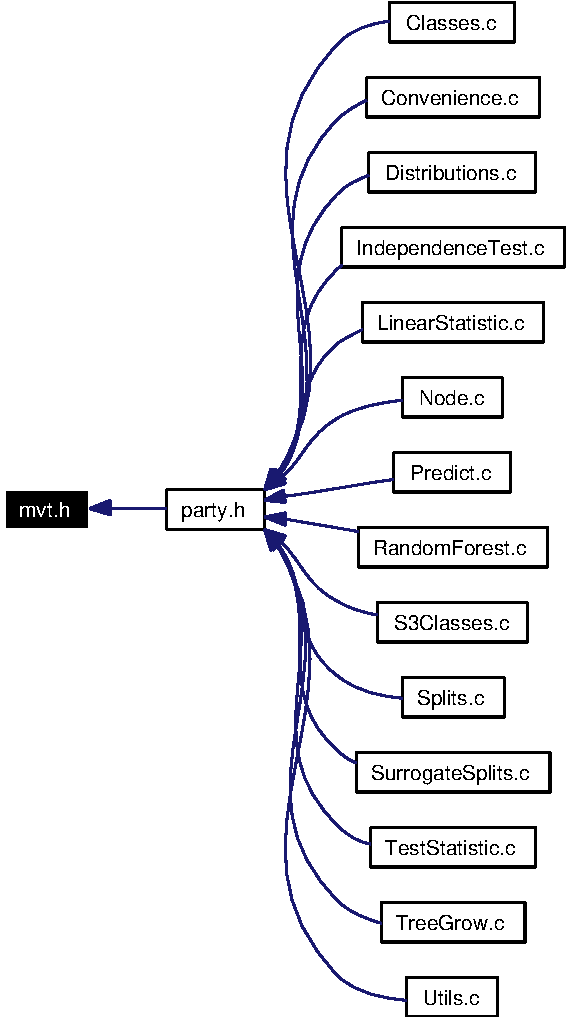
\includegraphics[width=420pt]{mvt_8h__dep__incl}
\end{center}
\end{figure}
\subsection*{Functions}
\begin{CompactItemize}
\item 
void F77\_\-NAME() \hyperlink{mvt_8h_2a7ae850a24d2fe1a610ca397d6871c7}{mvtdst} (int $\ast$n, int $\ast$nu, double $\ast$lower, double $\ast$upper, int $\ast$infin, double $\ast$corr, double $\ast$delta, int $\ast$maxpts, double $\ast$abseps, double $\ast$releps, double $\ast$error, double $\ast$value, int $\ast$inform)
\end{CompactItemize}


\subsection{Function Documentation}
\hypertarget{mvt_8h_2a7ae850a24d2fe1a610ca397d6871c7}{
\index{mvt.h@{mvt.h}!mvtdst@{mvtdst}}
\index{mvtdst@{mvtdst}!mvt.h@{mvt.h}}
\subsubsection[mvtdst]{\setlength{\rightskip}{0pt plus 5cm}void F77\_\-NAME() mvtdst (int $\ast$ {\em n}, \/  int $\ast$ {\em nu}, \/  double $\ast$ {\em lower}, \/  double $\ast$ {\em upper}, \/  int $\ast$ {\em infin}, \/  double $\ast$ {\em corr}, \/  double $\ast$ {\em delta}, \/  int $\ast$ {\em maxpts}, \/  double $\ast$ {\em abseps}, \/  double $\ast$ {\em releps}, \/  double $\ast$ {\em error}, \/  double $\ast$ {\em value}, \/  int $\ast$ {\em inform})}}
\label{mvt_8h_2a7ae850a24d2fe1a610ca397d6871c7}




Referenced by C\_\-maxabsConditionalPvalue().
\hypertarget{Node_8c}{
\section{Node.c File Reference}
\label{Node_8c}\index{Node.c@{Node.c}}
}
{\tt \#include \char`\"{}party.h\char`\"{}}\par


Include dependency graph for Node.c:\begin{figure}[H]
\begin{center}
\leavevmode
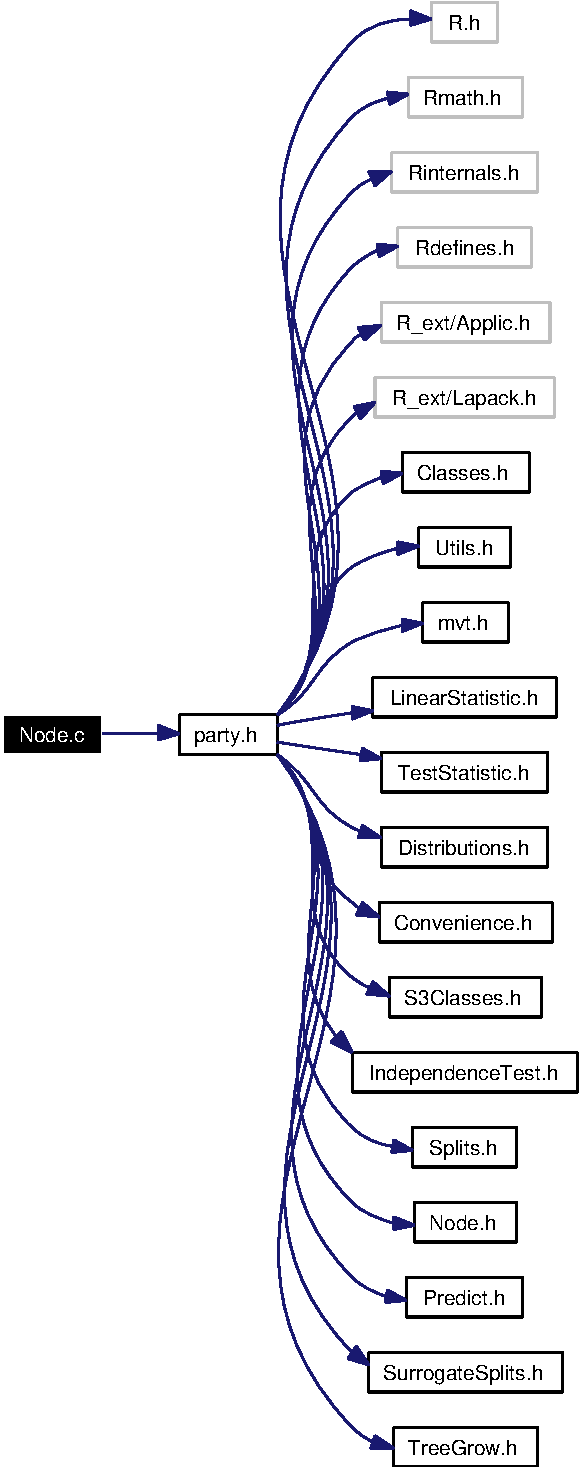
\includegraphics[width=156pt]{Node_8c__incl}
\end{center}
\end{figure}
\subsection*{Functions}
\begin{CompactItemize}
\item 
void \hyperlink{Node_8c_a0}{C\_\-prediction} (const double $\ast$y, int n, int q, const double $\ast$weights, const double sweights, double $\ast$ans)
\item 
void \hyperlink{Node_8c_a1}{C\_\-Node} (SEXP node, SEXP learnsample, SEXP weights, SEXP fitmem, SEXP controls, int TERMINAL)
\item 
SEXP \hyperlink{Node_8c_a2}{R\_\-Node} (SEXP learnsample, SEXP weights, SEXP fitmem, SEXP controls)
\end{CompactItemize}


\subsection{Detailed Description}
Node computations

\begin{Desc}
\item[Author:]\begin{Desc}
\item[Author]hothorn \end{Desc}
\end{Desc}
\begin{Desc}
\item[Date:]\begin{Desc}
\item[Date]2005-10-19 16:40:43 +0200 (Wed, 19 Oct 2005) \end{Desc}
\end{Desc}


Definition in file \hyperlink{Node_8c-source}{Node.c}.

\subsection{Function Documentation}
\hypertarget{Node_8c_a1}{
\index{Node.c@{Node.c}!C_Node@{C\_\-Node}}
\index{C_Node@{C\_\-Node}!Node.c@{Node.c}}
\subsubsection[C\_\-Node]{\setlength{\rightskip}{0pt plus 5cm}void C\_\-Node (SEXP {\em node}, SEXP {\em learnsample}, SEXP {\em weights}, SEXP {\em fitmem}, SEXP {\em controls}, int {\em TERMINAL})}}
\label{Node_8c_a1}


The main function for all node computations \begin{Desc}
\item[Parameters:]
\begin{description}
\item[{\em node}]an initialized node (an S3 object!) \item[{\em learnsample}]an object of class `Learning\-Sample' \item[{\em weights}]case weights \item[{\em fitmem}]an object of class `Tree\-Fit\-Memory' \item[{\em controls}]an object of class `Tree\-Control' \item[{\em TERMINAL}]logical indicating if this node will be a terminal node \end{description}
\end{Desc}


Definition at line 48 of file Node.c.

References C\_\-Global\-Test(), C\_\-init\_\-nominalsplit(), C\_\-init\_\-orderedsplit(), C\_\-max(), C\_\-prediction(), C\_\-split(), C\_\-splitcategorical(), C\_\-standardize(), C\_\-whichmax(), get\_\-dimension(), get\_\-gtctrl(), get\_\-levels(), get\_\-mincriterion(), get\_\-minsplit(), get\_\-ninputs(), get\_\-nobs(), get\_\-ordering(), get\_\-savesplitstats(), get\_\-splitctrl(), get\_\-splitstatistics(), get\_\-tgctrl(), get\_\-tol(), get\_\-transformation(), get\_\-varctrl(), get\_\-variable(), get\_\-varmemory(), get\_\-weights(), has\_\-missings(), is\_\-nominal(), is\_\-ordinal(), ncol(), PL2\_\-covariance\-Sym, PL2\_\-expcovinf\-Sym, PL2\_\-expectation\-Sym, PL2\_\-inputs\-Sym, PL2\_\-jointtransf\-Sym, PL2\_\-linearstatistic\-Sym, PL2\_\-linexpcov2sample\-Sym, PL2\_\-responses\-Sym, PL2\_\-scores\-Sym, PL2\_\-sumweights\-Sym, S3get\_\-criterion(), S3get\_\-maxcriterion(), S3get\_\-prediction(), S3get\_\-primarysplit(), S3get\_\-splitpoint(), S3get\_\-splitstatistics(), S3get\_\-table(), S3get\_\-teststat(), S3set\_\-nodeterminal(), and S3set\_\-variable\-ID().

Referenced by C\_\-Tree\-Grow(), and R\_\-Node().

Here is the call graph for this function:\begin{figure}[H]
\begin{center}
\leavevmode
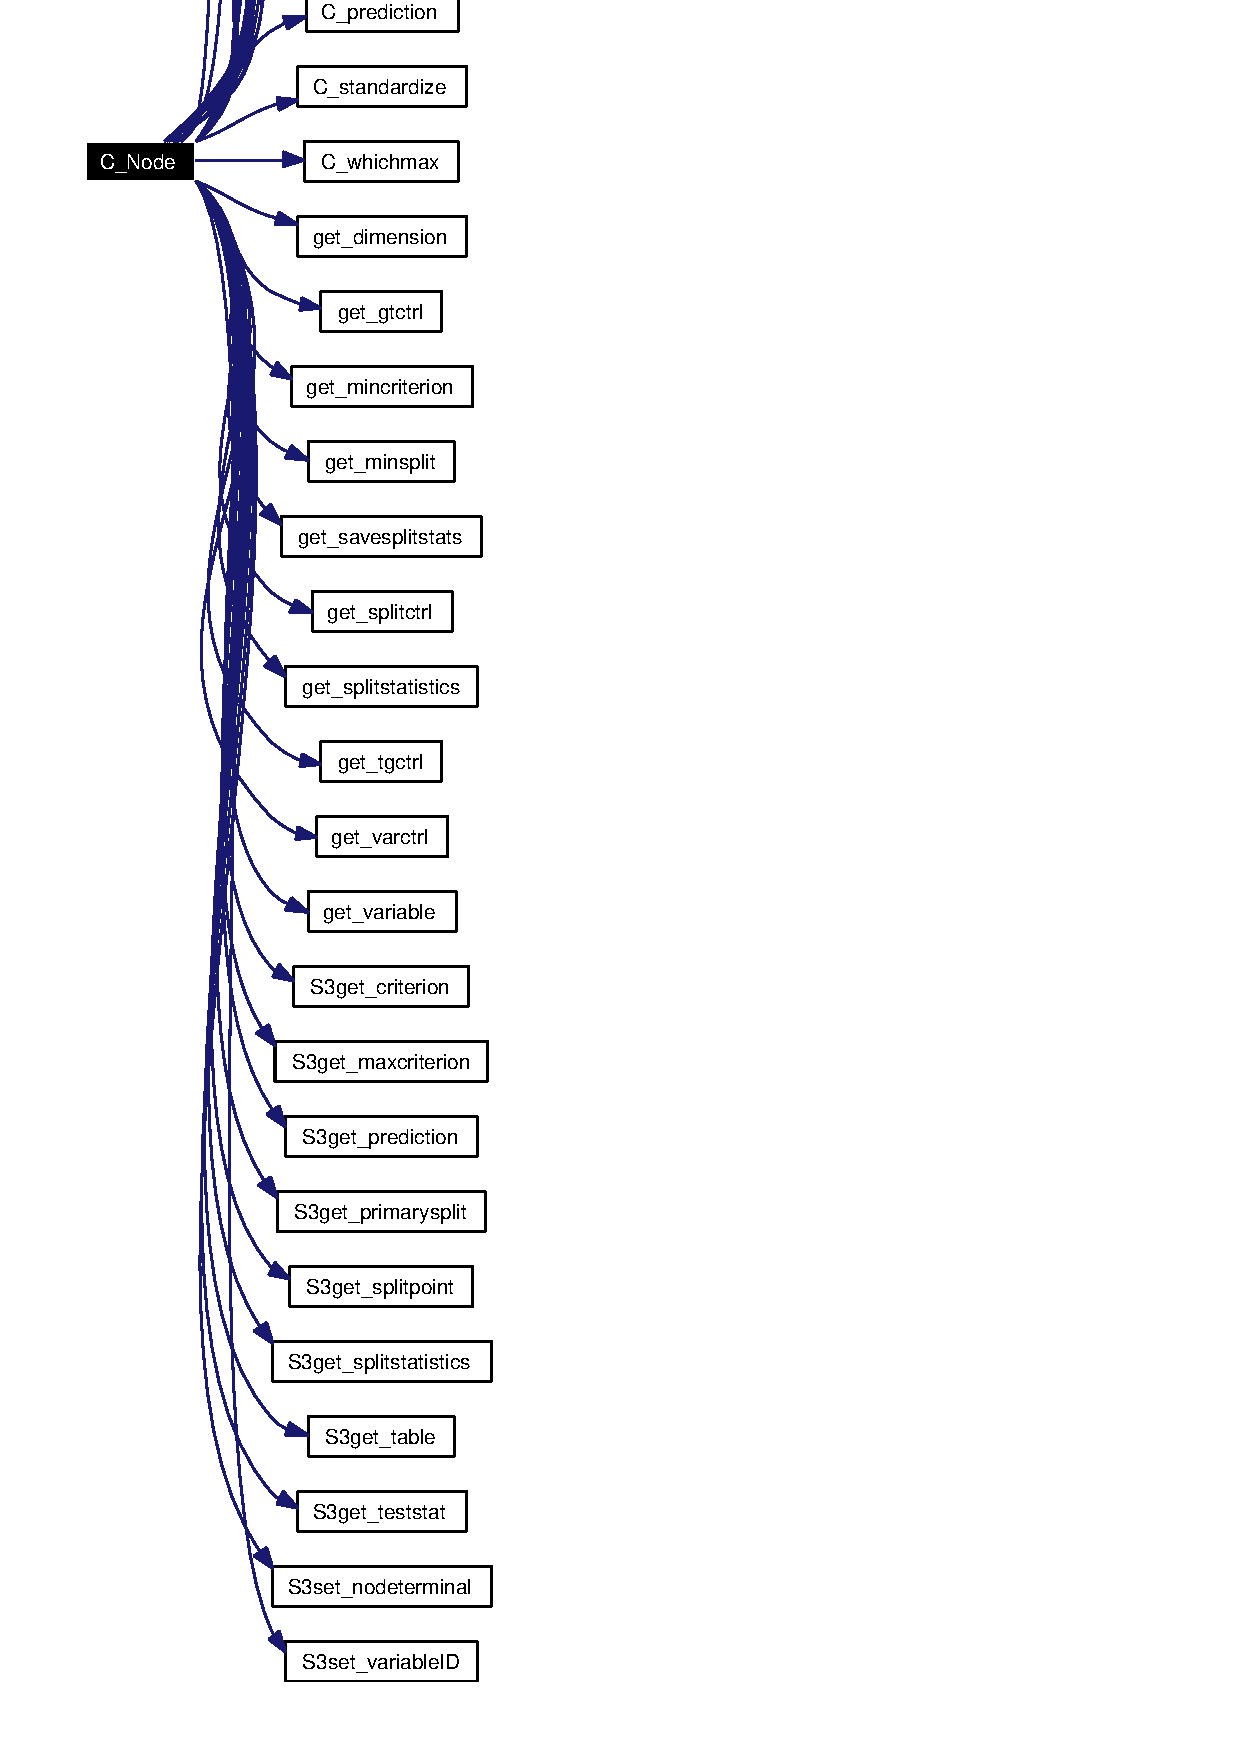
\includegraphics[width=231pt]{Node_8c_a1_cgraph}
\end{center}
\end{figure}
\hypertarget{Node_8c_a0}{
\index{Node.c@{Node.c}!C_prediction@{C\_\-prediction}}
\index{C_prediction@{C\_\-prediction}!Node.c@{Node.c}}
\subsubsection[C\_\-prediction]{\setlength{\rightskip}{0pt plus 5cm}void C\_\-prediction (const double $\ast$ {\em y}, int {\em n}, int {\em q}, const double $\ast$ {\em weights}, const double {\em sweights}, double $\ast$ {\em ans})}}
\label{Node_8c_a0}


Compute prediction of a node \begin{Desc}
\item[Parameters:]
\begin{description}
\item[{\em y}]the response variable (raw numeric values or dummy encoded factor) \item[{\em n}]number of observations \item[{\em q}]number of columns of y \item[{\em weights}]case weights \item[{\em sweights}]sum of case weights \item[{\em ans}]return value; the q-dimensional predictions \end{description}
\end{Desc}


Definition at line 22 of file Node.c.

Referenced by C\_\-Node().\hypertarget{Node_8c_a2}{
\index{Node.c@{Node.c}!R_Node@{R\_\-Node}}
\index{R_Node@{R\_\-Node}!Node.c@{Node.c}}
\subsubsection[R\_\-Node]{\setlength{\rightskip}{0pt plus 5cm}SEXP R\_\-Node (SEXP {\em learnsample}, SEXP {\em weights}, SEXP {\em fitmem}, SEXP {\em controls})}}
\label{Node_8c_a2}


R-interface to C\_\-Node \begin{Desc}
\item[Parameters:]
\begin{description}
\item[{\em learnsample}]an object of class `Learning\-Sample' \item[{\em weights}]case weights \item[{\em fitmem}]an object of class `Tree\-Fit\-Memory' \item[{\em controls}]an object of class `Tree\-Control' \end{description}
\end{Desc}


Definition at line 233 of file Node.c.

References C\_\-init\_\-node(), C\_\-Node(), get\_\-maxsurrogate(), get\_\-ninputs(), get\_\-nobs(), get\_\-splitctrl(), ncol(), NODE\_\-LENGTH, PL2\_\-jointtransf\-Sym, and PL2\_\-responses\-Sym.

Here is the call graph for this function:\begin{figure}[H]
\begin{center}
\leavevmode
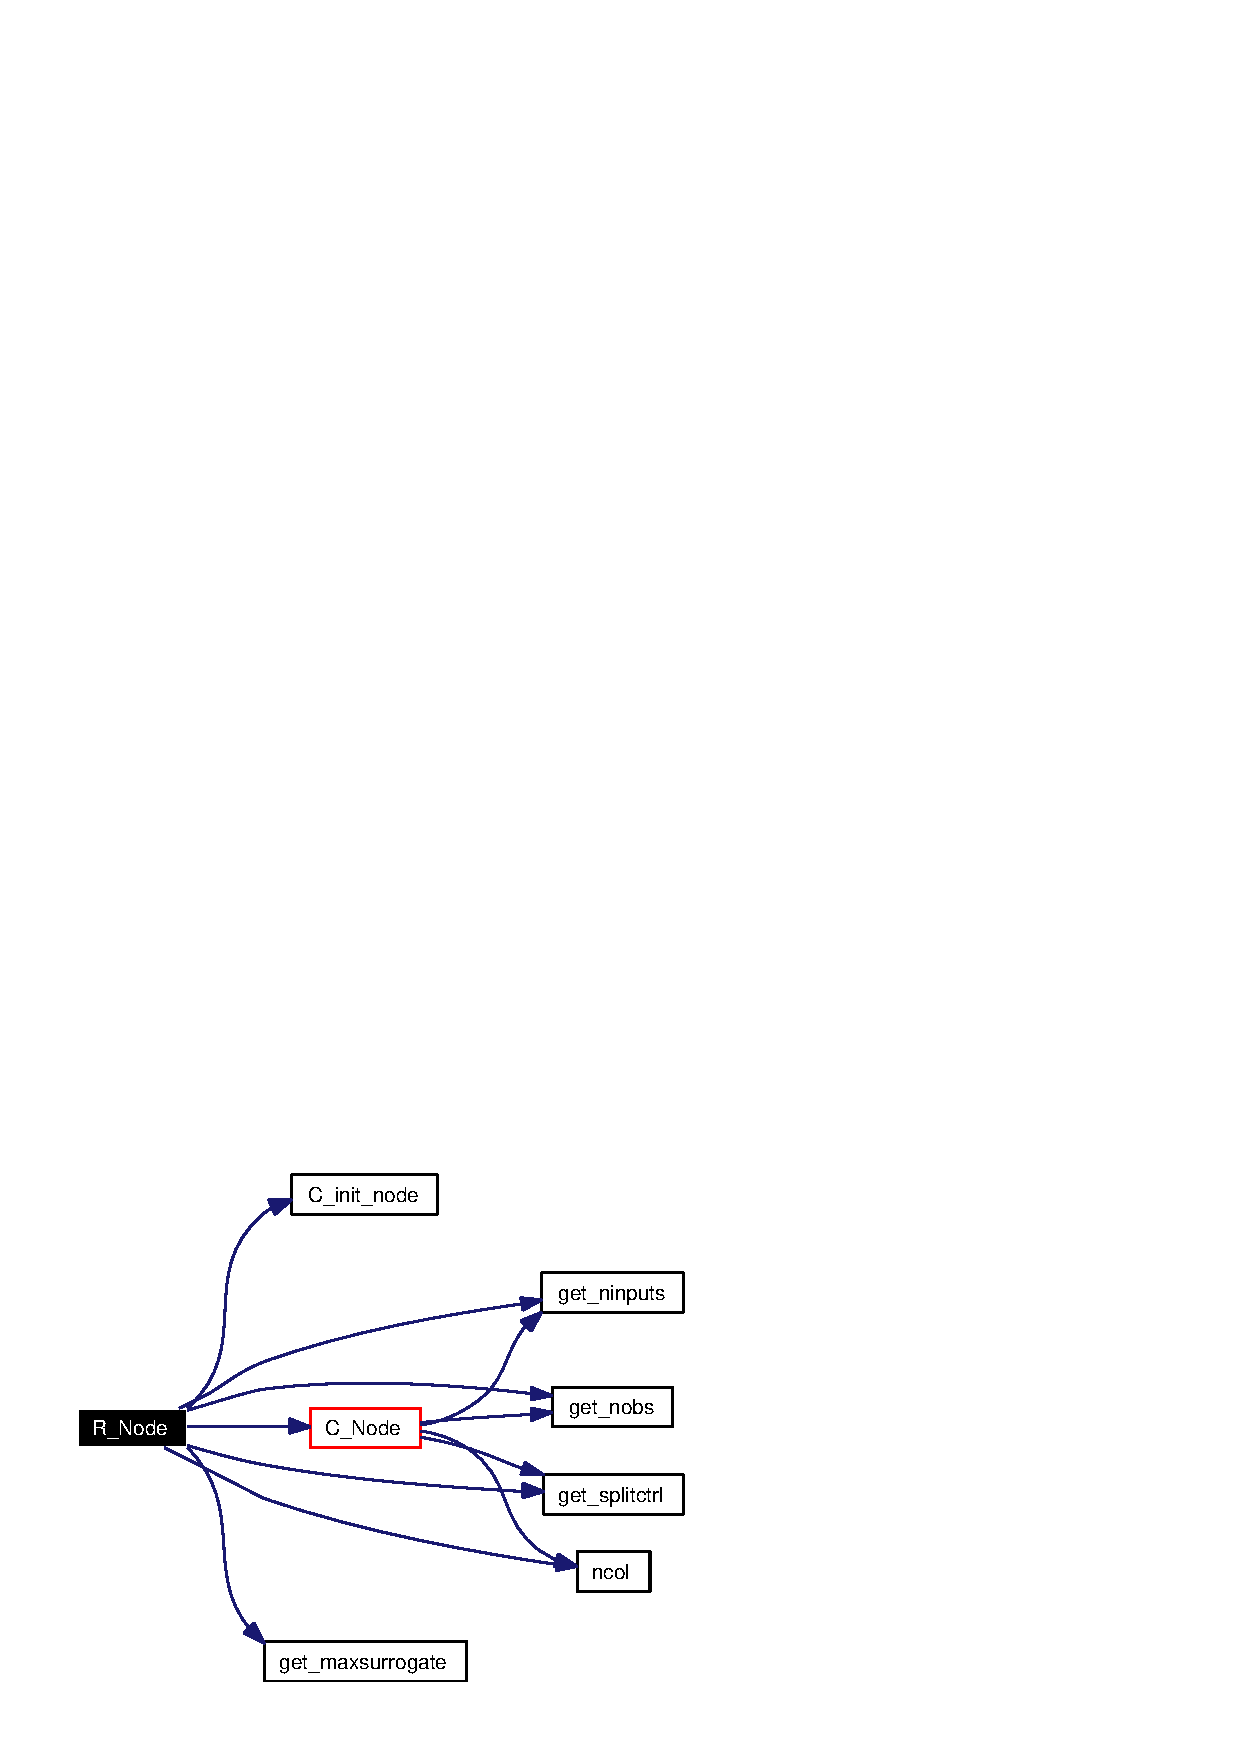
\includegraphics[width=169pt]{Node_8c_a2_cgraph}
\end{center}
\end{figure}

\hypertarget{Node_8h}{
\section{Node.h File Reference}
\label{Node_8h}\index{Node.h@{Node.h}}
}


This graph shows which files directly or indirectly include this file:\nopagebreak
\begin{figure}[H]
\begin{center}
\leavevmode
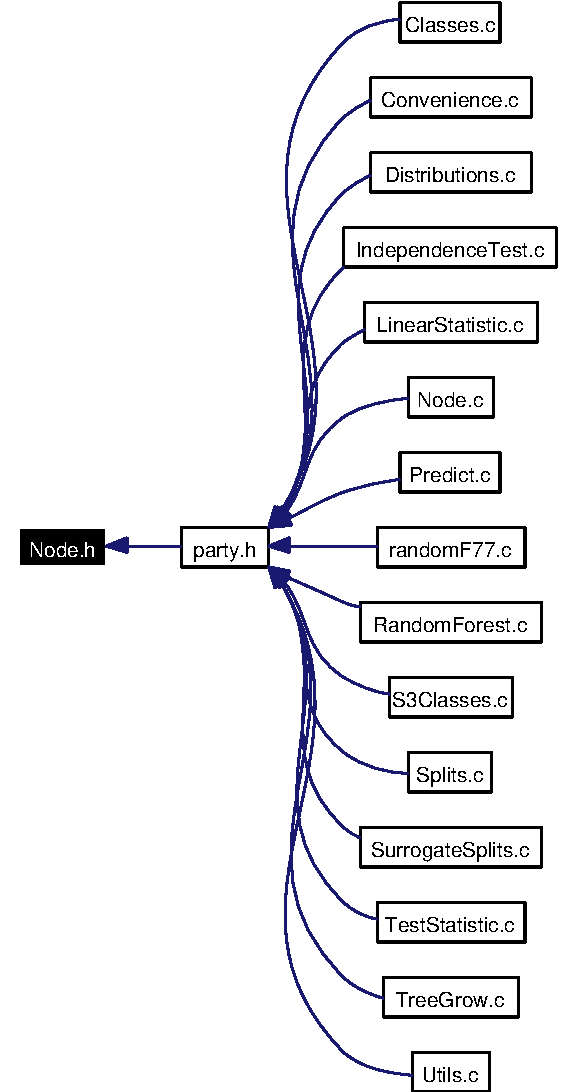
\includegraphics[width=420pt]{Node_8h__dep__incl}
\end{center}
\end{figure}
\subsection*{Functions}
\begin{CompactItemize}
\item 
void \hyperlink{Node_8h_0ed8b15b2c14ec9f1f1585d6288a38e2}{C\_\-Node} (SEXP node, SEXP learnsample, SEXP weights, SEXP fitmem, SEXP controls, int TERMINAL)
\end{CompactItemize}


\subsection{Function Documentation}
\hypertarget{Node_8h_0ed8b15b2c14ec9f1f1585d6288a38e2}{
\index{Node.h@{Node.h}!C\_\-Node@{C\_\-Node}}
\index{C\_\-Node@{C\_\-Node}!Node.h@{Node.h}}
\subsubsection[C\_\-Node]{\setlength{\rightskip}{0pt plus 5cm}void C\_\-Node (SEXP {\em node}, \/  SEXP {\em learnsample}, \/  SEXP {\em weights}, \/  SEXP {\em fitmem}, \/  SEXP {\em controls}, \/  int {\em TERMINAL})}}
\label{Node_8h_0ed8b15b2c14ec9f1f1585d6288a38e2}


The main function for all node computations \begin{Desc}
\item[Parameters:]
\begin{description}
\item[{\em node}]an initialized node (an S3 object!) \item[{\em learnsample}]an object of class `LearningSample' \item[{\em weights}]case weights \item[{\em fitmem}]an object of class `TreeFitMemory' \item[{\em controls}]an object of class `TreeControl' \item[{\em TERMINAL}]logical indicating if this node will be a terminal node \end{description}
\end{Desc}


Definition at line 48 of file Node.c.

References C\_\-GlobalTest(), C\_\-init\_\-nominalsplit(), C\_\-init\_\-orderedsplit(), C\_\-max(), C\_\-prediction(), C\_\-split(), C\_\-splitcategorical(), C\_\-standardize(), C\_\-tempweights(), C\_\-whichmax(), get\_\-dimension(), get\_\-gtctrl(), get\_\-levels(), get\_\-mincriterion(), get\_\-minsplit(), get\_\-ninputs(), get\_\-nobs(), get\_\-ordering(), get\_\-predict\_\-trafo(), get\_\-savesplitstats(), get\_\-splitctrl(), get\_\-splitstatistics(), get\_\-test\_\-trafo(), get\_\-tgctrl(), get\_\-tol(), get\_\-transformation(), get\_\-varctrl(), get\_\-variable(), get\_\-varmemory(), has\_\-missings(), is\_\-nominal(), ncol(), PL2\_\-covarianceSym, PL2\_\-expcovinfSym, PL2\_\-expectationSym, PL2\_\-inputsSym, PL2\_\-linearstatisticSym, PL2\_\-linexpcov2sampleSym, PL2\_\-responsesSym, PL2\_\-sumweightsSym, S3\_\-SUMWEIGHTS, S3get\_\-criterion(), S3get\_\-maxcriterion(), S3get\_\-prediction(), S3get\_\-primarysplit(), S3get\_\-splitpoint(), S3get\_\-splitstatistics(), S3get\_\-table(), S3get\_\-teststat(), S3set\_\-nodeterminal(), and S3set\_\-variableID().

Referenced by C\_\-TreeGrow(), and R\_\-Node().

Here is the call graph for this function:\nopagebreak
\begin{figure}[H]
\begin{center}
\leavevmode
\includegraphics[width=278pt]{Node_8h_0ed8b15b2c14ec9f1f1585d6288a38e2_cgraph}
\end{center}
\end{figure}

\hypertarget{party_8h}{
\section{party.h File Reference}
\label{party_8h}\index{party.h@{party.h}}
}
{\tt \#include $<$R.h$>$}\par
{\tt \#include $<$Rmath.h$>$}\par
{\tt \#include $<$Rinternals.h$>$}\par
{\tt \#include $<$Rdefines.h$>$}\par
{\tt \#include $<$R\_\-ext/Applic.h$>$}\par
{\tt \#include \char`\"{}Classes.h\char`\"{}}\par
{\tt \#include \char`\"{}Utils.h\char`\"{}}\par
{\tt \#include \char`\"{}mvt.h\char`\"{}}\par
{\tt \#include \char`\"{}Linear\-Statistic.h\char`\"{}}\par
{\tt \#include \char`\"{}Test\-Statistic.h\char`\"{}}\par
{\tt \#include \char`\"{}Distributions.h\char`\"{}}\par
{\tt \#include \char`\"{}Convenience.h\char`\"{}}\par
{\tt \#include \char`\"{}S3Classes.h\char`\"{}}\par
{\tt \#include \char`\"{}Independence\-Test.h\char`\"{}}\par
{\tt \#include \char`\"{}Splits.h\char`\"{}}\par
{\tt \#include \char`\"{}Node.h\char`\"{}}\par
{\tt \#include \char`\"{}Predict.h\char`\"{}}\par
{\tt \#include \char`\"{}Surrogate\-Splits.h\char`\"{}}\par


Include dependency graph for party.h:\begin{figure}[H]
\begin{center}
\leavevmode
\includegraphics[width=118pt]{party_8h__incl}
\end{center}
\end{figure}


This graph shows which files directly or indirectly include this file:\begin{figure}[H]
\begin{center}
\leavevmode
\includegraphics[width=116pt]{party_8h__dep__incl}
\end{center}
\end{figure}
\subsection*{Defines}
\begin{CompactItemize}
\item 
\#define \hyperlink{party_8h_a0}{S3\_\-NODEID}~0
\item 
\#define \hyperlink{party_8h_a1}{S3\_\-WEIGHTS}~1
\item 
\#define \hyperlink{party_8h_a2}{S3\_\-CRITERION}~2
\item 
\#define \hyperlink{party_8h_a3}{S3\_\-TERMINAL}~3
\item 
\#define \hyperlink{party_8h_a4}{S3\_\-PSPLIT}~4
\item 
\#define \hyperlink{party_8h_a5}{S3\_\-SSPLIT}~5
\item 
\#define \hyperlink{party_8h_a6}{S3\_\-PREDICTION}~6
\item 
\#define \hyperlink{party_8h_a7}{S3\_\-LEFT}~7
\item 
\#define \hyperlink{party_8h_a8}{S3\_\-RIGHT}~8
\item 
\#define \hyperlink{party_8h_a9}{NODE\_\-LENGTH}~9
\item 
\#define \hyperlink{party_8h_a10}{S3\_\-STATISTICS}~0
\item 
\#define \hyperlink{party_8h_a11}{S3\_\-i\-CRITERION}~1
\item 
\#define \hyperlink{party_8h_a12}{S3\_\-MAXCRITERION}~2
\item 
\#define \hyperlink{party_8h_a13}{CRITERION\_\-LENGTH}~3
\item 
\#define \hyperlink{party_8h_a14}{S3\_\-VARIABLEID}~0
\item 
\#define \hyperlink{party_8h_a15}{S3\_\-ORDERED}~1
\item 
\#define \hyperlink{party_8h_a16}{S3\_\-SPLITPOINT}~2
\item 
\#define \hyperlink{party_8h_a17}{S3\_\-SPLITSTATISTICS}~3
\item 
\#define \hyperlink{party_8h_a18}{S3\_\-TOLEFT}~4
\item 
\#define \hyperlink{party_8h_a19}{SPLIT\_\-LENGTH}~5
\item 
\#define \hyperlink{party_8h_a20}{MAXABS}~1
\item 
\#define \hyperlink{party_8h_a21}{QUADFORM}~2
\item 
\#define \hyperlink{party_8h_a22}{BONFERRONI}~1
\item 
\#define \hyperlink{party_8h_a23}{MONTECARLO}~2
\item 
\#define \hyperlink{party_8h_a24}{AGGREGATED}~3
\item 
\#define \hyperlink{party_8h_a25}{RAW}~4
\end{CompactItemize}


\subsection{Define Documentation}
\hypertarget{party_8h_a24}{
\index{party.h@{party.h}!AGGREGATED@{AGGREGATED}}
\index{AGGREGATED@{AGGREGATED}!party.h@{party.h}}
\subsubsection[AGGREGATED]{\setlength{\rightskip}{0pt plus 5cm}\#define AGGREGATED~3}}
\label{party_8h_a24}




Definition at line 64 of file party.h.

Referenced by C\_\-Global\-Test().\hypertarget{party_8h_a22}{
\index{party.h@{party.h}!BONFERRONI@{BONFERRONI}}
\index{BONFERRONI@{BONFERRONI}!party.h@{party.h}}
\subsubsection[BONFERRONI]{\setlength{\rightskip}{0pt plus 5cm}\#define BONFERRONI~1}}
\label{party_8h_a22}




Definition at line 62 of file party.h.

Referenced by C\_\-Global\-Test().\hypertarget{party_8h_a13}{
\index{party.h@{party.h}!CRITERION_LENGTH@{CRITERION\_\-LENGTH}}
\index{CRITERION_LENGTH@{CRITERION\_\-LENGTH}!party.h@{party.h}}
\subsubsection[CRITERION\_\-LENGTH]{\setlength{\rightskip}{0pt plus 5cm}\#define CRITERION\_\-LENGTH~3}}
\label{party_8h_a13}




Definition at line 47 of file party.h.

Referenced by C\_\-init\_\-node().\hypertarget{party_8h_a20}{
\index{party.h@{party.h}!MAXABS@{MAXABS}}
\index{MAXABS@{MAXABS}!party.h@{party.h}}
\subsubsection[MAXABS]{\setlength{\rightskip}{0pt plus 5cm}\#define MAXABS~1}}
\label{party_8h_a20}




Definition at line 58 of file party.h.

Referenced by C\_\-Conditional\-Pvalue().\hypertarget{party_8h_a23}{
\index{party.h@{party.h}!MONTECARLO@{MONTECARLO}}
\index{MONTECARLO@{MONTECARLO}!party.h@{party.h}}
\subsubsection[MONTECARLO]{\setlength{\rightskip}{0pt plus 5cm}\#define MONTECARLO~2}}
\label{party_8h_a23}




Definition at line 63 of file party.h.

Referenced by C\_\-Global\-Test().\hypertarget{party_8h_a9}{
\index{party.h@{party.h}!NODE_LENGTH@{NODE\_\-LENGTH}}
\index{NODE_LENGTH@{NODE\_\-LENGTH}!party.h@{party.h}}
\subsubsection[NODE\_\-LENGTH]{\setlength{\rightskip}{0pt plus 5cm}\#define NODE\_\-LENGTH~9}}
\label{party_8h_a9}




Definition at line 41 of file party.h.

Referenced by C\_\-init\_\-node(), C\_\-splitnode(), R\_\-Ensemble(), R\_\-Node(), and R\_\-Tree\-Grow().\hypertarget{party_8h_a21}{
\index{party.h@{party.h}!QUADFORM@{QUADFORM}}
\index{QUADFORM@{QUADFORM}!party.h@{party.h}}
\subsubsection[QUADFORM]{\setlength{\rightskip}{0pt plus 5cm}\#define QUADFORM~2}}
\label{party_8h_a21}




Definition at line 59 of file party.h.

Referenced by C\_\-Conditional\-Pvalue().\hypertarget{party_8h_a25}{
\index{party.h@{party.h}!RAW@{RAW}}
\index{RAW@{RAW}!party.h@{party.h}}
\subsubsection[RAW]{\setlength{\rightskip}{0pt plus 5cm}\#define RAW~4}}
\label{party_8h_a25}




Definition at line 65 of file party.h.

Referenced by C\_\-Global\-Test().\hypertarget{party_8h_a2}{
\index{party.h@{party.h}!S3_CRITERION@{S3\_\-CRITERION}}
\index{S3_CRITERION@{S3\_\-CRITERION}!party.h@{party.h}}
\subsubsection[S3\_\-CRITERION]{\setlength{\rightskip}{0pt plus 5cm}\#define S3\_\-CRITERION~2}}
\label{party_8h_a2}




Definition at line 34 of file party.h.

Referenced by C\_\-init\_\-node(), S3get\_\-criterion(), S3get\_\-maxcriterion(), and S3get\_\-teststat().\hypertarget{party_8h_a11}{
\index{party.h@{party.h}!S3_iCRITERION@{S3\_\-iCRITERION}}
\index{S3_iCRITERION@{S3\_\-iCRITERION}!party.h@{party.h}}
\subsubsection[S3\_\-iCRITERION]{\setlength{\rightskip}{0pt plus 5cm}\#define S3\_\-i\-CRITERION~1}}
\label{party_8h_a11}




Definition at line 45 of file party.h.

Referenced by C\_\-init\_\-node(), and S3get\_\-criterion().\hypertarget{party_8h_a7}{
\index{party.h@{party.h}!S3_LEFT@{S3\_\-LEFT}}
\index{S3_LEFT@{S3\_\-LEFT}!party.h@{party.h}}
\subsubsection[S3\_\-LEFT]{\setlength{\rightskip}{0pt plus 5cm}\#define S3\_\-LEFT~7}}
\label{party_8h_a7}




Definition at line 39 of file party.h.

Referenced by C\_\-splitnode(), and S3get\_\-leftnode().\hypertarget{party_8h_a12}{
\index{party.h@{party.h}!S3_MAXCRITERION@{S3\_\-MAXCRITERION}}
\index{S3_MAXCRITERION@{S3\_\-MAXCRITERION}!party.h@{party.h}}
\subsubsection[S3\_\-MAXCRITERION]{\setlength{\rightskip}{0pt plus 5cm}\#define S3\_\-MAXCRITERION~2}}
\label{party_8h_a12}




Definition at line 46 of file party.h.

Referenced by C\_\-init\_\-node(), and S3get\_\-maxcriterion().\hypertarget{party_8h_a0}{
\index{party.h@{party.h}!S3_NODEID@{S3\_\-NODEID}}
\index{S3_NODEID@{S3\_\-NODEID}!party.h@{party.h}}
\subsubsection[S3\_\-NODEID]{\setlength{\rightskip}{0pt plus 5cm}\#define S3\_\-NODEID~0}}
\label{party_8h_a0}




Definition at line 32 of file party.h.

Referenced by C\_\-init\_\-node(), S3get\_\-node\-ID(), and S3set\_\-node\-ID().\hypertarget{party_8h_a15}{
\index{party.h@{party.h}!S3_ORDERED@{S3\_\-ORDERED}}
\index{S3_ORDERED@{S3\_\-ORDERED}!party.h@{party.h}}
\subsubsection[S3\_\-ORDERED]{\setlength{\rightskip}{0pt plus 5cm}\#define S3\_\-ORDERED~1}}
\label{party_8h_a15}




Definition at line 51 of file party.h.

Referenced by C\_\-init\_\-nominalsplit(), C\_\-init\_\-orderedsplit(), S3is\_\-ordered(), S3set\_\-nominal(), and S3set\_\-ordered().\hypertarget{party_8h_a6}{
\index{party.h@{party.h}!S3_PREDICTION@{S3\_\-PREDICTION}}
\index{S3_PREDICTION@{S3\_\-PREDICTION}!party.h@{party.h}}
\subsubsection[S3\_\-PREDICTION]{\setlength{\rightskip}{0pt plus 5cm}\#define S3\_\-PREDICTION~6}}
\label{party_8h_a6}




Definition at line 38 of file party.h.

Referenced by C\_\-init\_\-node(), and S3get\_\-prediction().\hypertarget{party_8h_a4}{
\index{party.h@{party.h}!S3_PSPLIT@{S3\_\-PSPLIT}}
\index{S3_PSPLIT@{S3\_\-PSPLIT}!party.h@{party.h}}
\subsubsection[S3\_\-PSPLIT]{\setlength{\rightskip}{0pt plus 5cm}\#define S3\_\-PSPLIT~4}}
\label{party_8h_a4}




Definition at line 36 of file party.h.

Referenced by C\_\-init\_\-node(), and S3get\_\-primarysplit().\hypertarget{party_8h_a8}{
\index{party.h@{party.h}!S3_RIGHT@{S3\_\-RIGHT}}
\index{S3_RIGHT@{S3\_\-RIGHT}!party.h@{party.h}}
\subsubsection[S3\_\-RIGHT]{\setlength{\rightskip}{0pt plus 5cm}\#define S3\_\-RIGHT~8}}
\label{party_8h_a8}




Definition at line 40 of file party.h.

Referenced by C\_\-splitnode(), and S3get\_\-rightnode().\hypertarget{party_8h_a16}{
\index{party.h@{party.h}!S3_SPLITPOINT@{S3\_\-SPLITPOINT}}
\index{S3_SPLITPOINT@{S3\_\-SPLITPOINT}!party.h@{party.h}}
\subsubsection[S3\_\-SPLITPOINT]{\setlength{\rightskip}{0pt plus 5cm}\#define S3\_\-SPLITPOINT~2}}
\label{party_8h_a16}




Definition at line 52 of file party.h.

Referenced by C\_\-init\_\-nominalsplit(), C\_\-init\_\-orderedsplit(), and S3get\_\-splitpoint().\hypertarget{party_8h_a17}{
\index{party.h@{party.h}!S3_SPLITSTATISTICS@{S3\_\-SPLITSTATISTICS}}
\index{S3_SPLITSTATISTICS@{S3\_\-SPLITSTATISTICS}!party.h@{party.h}}
\subsubsection[S3\_\-SPLITSTATISTICS]{\setlength{\rightskip}{0pt plus 5cm}\#define S3\_\-SPLITSTATISTICS~3}}
\label{party_8h_a17}




Definition at line 53 of file party.h.

Referenced by C\_\-init\_\-nominalsplit(), C\_\-init\_\-orderedsplit(), and S3get\_\-splitstatistics().\hypertarget{party_8h_a5}{
\index{party.h@{party.h}!S3_SSPLIT@{S3\_\-SSPLIT}}
\index{S3_SSPLIT@{S3\_\-SSPLIT}!party.h@{party.h}}
\subsubsection[S3\_\-SSPLIT]{\setlength{\rightskip}{0pt plus 5cm}\#define S3\_\-SSPLIT~5}}
\label{party_8h_a5}




Definition at line 37 of file party.h.

Referenced by C\_\-init\_\-node(), and S3get\_\-surrogatesplits().\hypertarget{party_8h_a10}{
\index{party.h@{party.h}!S3_STATISTICS@{S3\_\-STATISTICS}}
\index{S3_STATISTICS@{S3\_\-STATISTICS}!party.h@{party.h}}
\subsubsection[S3\_\-STATISTICS]{\setlength{\rightskip}{0pt plus 5cm}\#define S3\_\-STATISTICS~0}}
\label{party_8h_a10}




Definition at line 44 of file party.h.

Referenced by C\_\-init\_\-node(), and S3get\_\-teststat().\hypertarget{party_8h_a3}{
\index{party.h@{party.h}!S3_TERMINAL@{S3\_\-TERMINAL}}
\index{S3_TERMINAL@{S3\_\-TERMINAL}!party.h@{party.h}}
\subsubsection[S3\_\-TERMINAL]{\setlength{\rightskip}{0pt plus 5cm}\#define S3\_\-TERMINAL~3}}
\label{party_8h_a3}




Definition at line 35 of file party.h.

Referenced by C\_\-init\_\-node(), S3get\_\-nodeterminal(), and S3set\_\-nodeterminal().\hypertarget{party_8h_a18}{
\index{party.h@{party.h}!S3_TOLEFT@{S3\_\-TOLEFT}}
\index{S3_TOLEFT@{S3\_\-TOLEFT}!party.h@{party.h}}
\subsubsection[S3\_\-TOLEFT]{\setlength{\rightskip}{0pt plus 5cm}\#define S3\_\-TOLEFT~4}}
\label{party_8h_a18}




Definition at line 54 of file party.h.

Referenced by C\_\-init\_\-nominalsplit(), C\_\-init\_\-orderedsplit(), S3get\_\-toleft(), and S3set\_\-toleft().\hypertarget{party_8h_a14}{
\index{party.h@{party.h}!S3_VARIABLEID@{S3\_\-VARIABLEID}}
\index{S3_VARIABLEID@{S3\_\-VARIABLEID}!party.h@{party.h}}
\subsubsection[S3\_\-VARIABLEID]{\setlength{\rightskip}{0pt plus 5cm}\#define S3\_\-VARIABLEID~0}}
\label{party_8h_a14}




Definition at line 50 of file party.h.

Referenced by C\_\-init\_\-nominalsplit(), C\_\-init\_\-orderedsplit(), S3get\_\-variable\-ID(), and S3set\_\-variable\-ID().\hypertarget{party_8h_a1}{
\index{party.h@{party.h}!S3_WEIGHTS@{S3\_\-WEIGHTS}}
\index{S3_WEIGHTS@{S3\_\-WEIGHTS}!party.h@{party.h}}
\subsubsection[S3\_\-WEIGHTS]{\setlength{\rightskip}{0pt plus 5cm}\#define S3\_\-WEIGHTS~1}}
\label{party_8h_a1}




Definition at line 33 of file party.h.

Referenced by C\_\-init\_\-node(), and S3get\_\-nodeweights().\hypertarget{party_8h_a19}{
\index{party.h@{party.h}!SPLIT_LENGTH@{SPLIT\_\-LENGTH}}
\index{SPLIT_LENGTH@{SPLIT\_\-LENGTH}!party.h@{party.h}}
\subsubsection[SPLIT\_\-LENGTH]{\setlength{\rightskip}{0pt plus 5cm}\#define SPLIT\_\-LENGTH~5}}
\label{party_8h_a19}




Definition at line 55 of file party.h.

Referenced by C\_\-init\_\-node(), C\_\-init\_\-nominalsplit(), C\_\-init\_\-orderedsplit(), and C\_\-surrogates().
\hypertarget{Predict_8c}{
\section{Predict.c File Reference}
\label{Predict_8c}\index{Predict.c@{Predict.c}}
}
{\tt \#include \char`\"{}party.h\char`\"{}}\par


Include dependency graph for Predict.c:\begin{figure}[H]
\begin{center}
\leavevmode
\includegraphics[width=160pt]{Predict_8c__incl}
\end{center}
\end{figure}
\subsection*{Functions}
\begin{CompactItemize}
\item 
void \hyperlink{Predict_8c_daf8a0eb8790ebf14f0e265de164d50e}{C\_\-splitnode} (SEXP node, SEXP learnsample, SEXP control)
\item 
SEXP \hyperlink{Predict_8c_dcd61d38c7c43d241d09a600b70fe3c5}{C\_\-get\_\-node} (SEXP subtree, SEXP newinputs, double mincriterion, int numobs)
\item 
SEXP \hyperlink{Predict_8c_dec31e3aa985e0af16ccaeac31237640}{R\_\-get\_\-node} (SEXP subtree, SEXP newinputs, SEXP mincriterion, SEXP numobs)
\item 
SEXP \hyperlink{Predict_8c_201fdee9dc7e3e71e90ea6609ed353cb}{C\_\-get\_\-nodebynum} (SEXP subtree, int nodenum)
\item 
SEXP \hyperlink{Predict_8c_4a30a8aa916f294059b6e2cbcb9e29d5}{R\_\-get\_\-nodebynum} (SEXP subtree, SEXP nodenum)
\item 
SEXP \hyperlink{Predict_8c_c4f4e806a78c376b13802ed2cf1e7b65}{C\_\-get\_\-prediction} (SEXP subtree, SEXP newinputs, double mincriterion, int numobs)
\item 
SEXP \hyperlink{Predict_8c_cbb3e45d03e1b544c94bf639b191a953}{C\_\-get\_\-nodeweights} (SEXP subtree, SEXP newinputs, double mincriterion, int numobs)
\item 
int \hyperlink{Predict_8c_d9d49b6a210f5c09a2a1d1aa496859ce}{C\_\-get\_\-node\-ID} (SEXP subtree, SEXP newinputs, double mincriterion, int numobs)
\item 
SEXP \hyperlink{Predict_8c_c0668d268fe5a4bad29fbf4ead39c526}{R\_\-get\_\-node\-ID} (SEXP tree, SEXP newinputs, SEXP mincriterion)
\item 
void \hyperlink{Predict_8c_ac36eff20575604b5d7558d512601d64}{C\_\-predict} (SEXP tree, SEXP newinputs, double mincriterion, SEXP ans)
\item 
SEXP \hyperlink{Predict_8c_9a5170a24bc00b727527b80cec5ca60a}{R\_\-predict} (SEXP tree, SEXP newinputs, SEXP mincriterion)
\item 
void \hyperlink{Predict_8c_8964e7493ed9cb96c271b168b721e329}{C\_\-getpredictions} (SEXP tree, SEXP where, SEXP ans)
\item 
SEXP \hyperlink{Predict_8c_a508a31f1fd7cd3668ad81eb0d00dd66}{R\_\-getpredictions} (SEXP tree, SEXP where)
\item 
SEXP \hyperlink{Predict_8c_4f6966402677cec07284a3e1bc25660f}{R\_\-predict\-RF\_\-weights} (SEXP forest, SEXP where, SEXP weights, SEXP newinputs, SEXP mincriterion, SEXP oobpred)
\end{CompactItemize}


\subsection{Detailed Description}
Node splitting and prediction

\begin{Desc}
\item[Author:]\begin{Desc}
\item[Author]hothorn \end{Desc}
\end{Desc}
\begin{Desc}
\item[Date:]\begin{Desc}
\item[Date]2007-07-23 10:02:09 +0200 (Mon, 23 Jul 2007) \end{Desc}
\end{Desc}


Definition in file \hyperlink{Predict_8c-source}{Predict.c}.

\subsection{Function Documentation}
\hypertarget{Predict_8c_dcd61d38c7c43d241d09a600b70fe3c5}{
\index{Predict.c@{Predict.c}!C_get_node@{C\_\-get\_\-node}}
\index{C_get_node@{C\_\-get\_\-node}!Predict.c@{Predict.c}}
\subsubsection[C\_\-get\_\-node]{\setlength{\rightskip}{0pt plus 5cm}SEXP C\_\-get\_\-node (SEXP {\em subtree}, SEXP {\em newinputs}, double {\em mincriterion}, int {\em numobs})}}
\label{Predict_8c_dcd61d38c7c43d241d09a600b70fe3c5}


Get the terminal node for obs. number `numobs' of `newinputs' \par
 \begin{Desc}
\item[Parameters:]
\begin{description}
\item[{\em subtree}]a tree \item[{\em newinputs}]an object of class `Variable\-Frame' \item[{\em mincriterion}]overwrites mincriterion used for tree growing \item[{\em numobs}]observation number \end{description}
\end{Desc}
\begin{Desc}
\item[\hyperlink{todo__todo000002}{Todo}]handle surrogate splits \end{Desc}


Definition at line 120 of file Predict.c.

References C\_\-i\_\-in\_\-set(), get\_\-missings(), get\_\-variable(), has\_\-missings(), S3get\_\-leftnode(), S3get\_\-maxcriterion(), S3get\_\-nodeterminal(), S3get\_\-primarysplit(), S3get\_\-rightnode(), S3get\_\-splitpoint(), S3get\_\-sumweights(), S3get\_\-surrogatesplits(), S3get\_\-toleft(), S3get\_\-variable\-ID(), and S3is\_\-ordered().

Referenced by C\_\-get\_\-node\-ID(), C\_\-get\_\-nodeweights(), C\_\-get\_\-prediction(), and R\_\-get\_\-node().

Here is the call graph for this function:\begin{figure}[H]
\begin{center}
\leavevmode
\includegraphics[width=186pt]{Predict_8c_dcd61d38c7c43d241d09a600b70fe3c5_cgraph}
\end{center}
\end{figure}
\hypertarget{Predict_8c_201fdee9dc7e3e71e90ea6609ed353cb}{
\index{Predict.c@{Predict.c}!C_get_nodebynum@{C\_\-get\_\-nodebynum}}
\index{C_get_nodebynum@{C\_\-get\_\-nodebynum}!Predict.c@{Predict.c}}
\subsubsection[C\_\-get\_\-nodebynum]{\setlength{\rightskip}{0pt plus 5cm}SEXP C\_\-get\_\-nodebynum (SEXP {\em subtree}, int {\em nodenum})}}
\label{Predict_8c_201fdee9dc7e3e71e90ea6609ed353cb}


Get the node with node\-ID `nodenum' \par
 \begin{Desc}
\item[Parameters:]
\begin{description}
\item[{\em subtree}]a tree \item[{\em nodenum}]a node\-ID \end{description}
\end{Desc}


Definition at line 242 of file Predict.c.

References S3get\_\-leftnode(), S3get\_\-node\-ID(), S3get\_\-nodeterminal(), and S3get\_\-rightnode().

Referenced by C\_\-getpredictions(), R\_\-get\_\-nodebynum(), and R\_\-predict\-RF\_\-weights().

Here is the call graph for this function:\begin{figure}[H]
\begin{center}
\leavevmode
\includegraphics[width=140pt]{Predict_8c_201fdee9dc7e3e71e90ea6609ed353cb_cgraph}
\end{center}
\end{figure}
\hypertarget{Predict_8c_d9d49b6a210f5c09a2a1d1aa496859ce}{
\index{Predict.c@{Predict.c}!C_get_nodeID@{C\_\-get\_\-nodeID}}
\index{C_get_nodeID@{C\_\-get\_\-nodeID}!Predict.c@{Predict.c}}
\subsubsection[C\_\-get\_\-nodeID]{\setlength{\rightskip}{0pt plus 5cm}int C\_\-get\_\-node\-ID (SEXP {\em subtree}, SEXP {\em newinputs}, double {\em mincriterion}, int {\em numobs})}}
\label{Predict_8c_d9d49b6a210f5c09a2a1d1aa496859ce}


Get the node\-ID for a new observation \par
 \begin{Desc}
\item[Parameters:]
\begin{description}
\item[{\em subtree}]a tree \item[{\em newinputs}]an object of class `Variable\-Frame' \item[{\em mincriterion}]overwrites mincriterion used for tree growing \item[{\em numobs}]observation number \end{description}
\end{Desc}


Definition at line 306 of file Predict.c.

References C\_\-get\_\-node(), and S3get\_\-node\-ID().

Referenced by R\_\-get\_\-node\-ID(), and R\_\-predict\-RF\_\-weights().

Here is the call graph for this function:\begin{figure}[H]
\begin{center}
\leavevmode
\includegraphics[width=249pt]{Predict_8c_d9d49b6a210f5c09a2a1d1aa496859ce_cgraph}
\end{center}
\end{figure}
\hypertarget{Predict_8c_cbb3e45d03e1b544c94bf639b191a953}{
\index{Predict.c@{Predict.c}!C_get_nodeweights@{C\_\-get\_\-nodeweights}}
\index{C_get_nodeweights@{C\_\-get\_\-nodeweights}!Predict.c@{Predict.c}}
\subsubsection[C\_\-get\_\-nodeweights]{\setlength{\rightskip}{0pt plus 5cm}SEXP C\_\-get\_\-nodeweights (SEXP {\em subtree}, SEXP {\em newinputs}, double {\em mincriterion}, int {\em numobs})}}
\label{Predict_8c_cbb3e45d03e1b544c94bf639b191a953}


Get the weights for a new observation \par
 \begin{Desc}
\item[Parameters:]
\begin{description}
\item[{\em subtree}]a tree \item[{\em newinputs}]an object of class `Variable\-Frame' \item[{\em mincriterion}]overwrites mincriterion used for tree growing \item[{\em numobs}]observation number \end{description}
\end{Desc}


Definition at line 291 of file Predict.c.

References C\_\-get\_\-node(), and S3get\_\-nodeweights().

Here is the call graph for this function:\begin{figure}[H]
\begin{center}
\leavevmode
\includegraphics[width=273pt]{Predict_8c_cbb3e45d03e1b544c94bf639b191a953_cgraph}
\end{center}
\end{figure}
\hypertarget{Predict_8c_c4f4e806a78c376b13802ed2cf1e7b65}{
\index{Predict.c@{Predict.c}!C_get_prediction@{C\_\-get\_\-prediction}}
\index{C_get_prediction@{C\_\-get\_\-prediction}!Predict.c@{Predict.c}}
\subsubsection[C\_\-get\_\-prediction]{\setlength{\rightskip}{0pt plus 5cm}SEXP C\_\-get\_\-prediction (SEXP {\em subtree}, SEXP {\em newinputs}, double {\em mincriterion}, int {\em numobs})}}
\label{Predict_8c_c4f4e806a78c376b13802ed2cf1e7b65}


Get the prediction of a new observation\par
 \begin{Desc}
\item[Parameters:]
\begin{description}
\item[{\em subtree}]a tree \item[{\em newinputs}]an object of class `Variable\-Frame' \item[{\em mincriterion}]overwrites mincriterion used for tree growing \item[{\em numobs}]observation number \end{description}
\end{Desc}


Definition at line 276 of file Predict.c.

References C\_\-get\_\-node(), and S3get\_\-prediction().

Referenced by C\_\-predict().

Here is the call graph for this function:\begin{figure}[H]
\begin{center}
\leavevmode
\includegraphics[width=260pt]{Predict_8c_c4f4e806a78c376b13802ed2cf1e7b65_cgraph}
\end{center}
\end{figure}
\hypertarget{Predict_8c_8964e7493ed9cb96c271b168b721e329}{
\index{Predict.c@{Predict.c}!C_getpredictions@{C\_\-getpredictions}}
\index{C_getpredictions@{C\_\-getpredictions}!Predict.c@{Predict.c}}
\subsubsection[C\_\-getpredictions]{\setlength{\rightskip}{0pt plus 5cm}void C\_\-getpredictions (SEXP {\em tree}, SEXP {\em where}, SEXP {\em ans})}}
\label{Predict_8c_8964e7493ed9cb96c271b168b721e329}


Get the predictions from `where' nodes\par
 \begin{Desc}
\item[Parameters:]
\begin{description}
\item[{\em tree}]a tree \item[{\em where}]vector of node\-ID's \item[{\em ans}]return value \end{description}
\end{Desc}


Definition at line 384 of file Predict.c.

References C\_\-get\_\-nodebynum(), and S3get\_\-prediction().

Referenced by R\_\-getpredictions().

Here is the call graph for this function:\begin{figure}[H]
\begin{center}
\leavevmode
\includegraphics[width=204pt]{Predict_8c_8964e7493ed9cb96c271b168b721e329_cgraph}
\end{center}
\end{figure}
\hypertarget{Predict_8c_ac36eff20575604b5d7558d512601d64}{
\index{Predict.c@{Predict.c}!C_predict@{C\_\-predict}}
\index{C_predict@{C\_\-predict}!Predict.c@{Predict.c}}
\subsubsection[C\_\-predict]{\setlength{\rightskip}{0pt plus 5cm}void C\_\-predict (SEXP {\em tree}, SEXP {\em newinputs}, double {\em mincriterion}, SEXP {\em ans})}}
\label{Predict_8c_ac36eff20575604b5d7558d512601d64}


Get all predictions for `newinputs' \par
 \begin{Desc}
\item[Parameters:]
\begin{description}
\item[{\em tree}]a tree \item[{\em newinputs}]an object of class `Variable\-Frame' \item[{\em mincriterion}]overwrites mincriterion used for tree growing \item[{\em ans}]return value \end{description}
\end{Desc}


Definition at line 343 of file Predict.c.

References C\_\-get\_\-prediction(), and get\_\-nobs().

Referenced by R\_\-predict().

Here is the call graph for this function:\begin{figure}[H]
\begin{center}
\leavevmode
\includegraphics[width=308pt]{Predict_8c_ac36eff20575604b5d7558d512601d64_cgraph}
\end{center}
\end{figure}
\hypertarget{Predict_8c_daf8a0eb8790ebf14f0e265de164d50e}{
\index{Predict.c@{Predict.c}!C_splitnode@{C\_\-splitnode}}
\index{C_splitnode@{C\_\-splitnode}!Predict.c@{Predict.c}}
\subsubsection[C\_\-splitnode]{\setlength{\rightskip}{0pt plus 5cm}void C\_\-splitnode (SEXP {\em node}, SEXP {\em learnsample}, SEXP {\em control})}}
\label{Predict_8c_daf8a0eb8790ebf14f0e265de164d50e}


Split a node according to a splitting rule \par
 \begin{Desc}
\item[Parameters:]
\begin{description}
\item[{\em node}]the current node with primary split specified \item[{\em learnsample}]learning sample \item[{\em control}]an object of class `Tree\-Control' \end{description}
\end{Desc}
\begin{Desc}
\item[\hyperlink{todo__todo000001}{Todo}]outplace the splitting since there are at least 3 functions with nearly identical code \end{Desc}


Definition at line 21 of file Predict.c.

References C\_\-init\_\-node(), get\_\-maxsurrogate(), get\_\-missings(), get\_\-ninputs(), get\_\-nobs(), get\_\-predict\_\-trafo(), get\_\-splitctrl(), get\_\-variable(), has\_\-missings(), i\_\-in\_\-set(), ncol(), NODE\_\-LENGTH, PL2\_\-inputs\-Sym, PL2\_\-responses\-Sym, S3\_\-LEFT, S3\_\-RIGHT, S3get\_\-nodeweights(), S3get\_\-primarysplit(), S3get\_\-splitpoint(), S3get\_\-variable\-ID(), and S3is\_\-ordered().

Referenced by C\_\-Tree\-Grow().

Here is the call graph for this function:\begin{figure}[H]
\begin{center}
\leavevmode
\includegraphics[width=180pt]{Predict_8c_daf8a0eb8790ebf14f0e265de164d50e_cgraph}
\end{center}
\end{figure}
\hypertarget{Predict_8c_dec31e3aa985e0af16ccaeac31237640}{
\index{Predict.c@{Predict.c}!R_get_node@{R\_\-get\_\-node}}
\index{R_get_node@{R\_\-get\_\-node}!Predict.c@{Predict.c}}
\subsubsection[R\_\-get\_\-node]{\setlength{\rightskip}{0pt plus 5cm}SEXP R\_\-get\_\-node (SEXP {\em subtree}, SEXP {\em newinputs}, SEXP {\em mincriterion}, SEXP {\em numobs})}}
\label{Predict_8c_dec31e3aa985e0af16ccaeac31237640}


R-Interface to C\_\-get\_\-node \par
 \begin{Desc}
\item[Parameters:]
\begin{description}
\item[{\em subtree}]a tree \item[{\em newinputs}]an object of class `Variable\-Frame' \item[{\em mincriterion}]overwrites mincriterion used for tree growing \item[{\em numobs}]observation number \end{description}
\end{Desc}


Definition at line 229 of file Predict.c.

References C\_\-get\_\-node().

Here is the call graph for this function:\begin{figure}[H]
\begin{center}
\leavevmode
\includegraphics[width=240pt]{Predict_8c_dec31e3aa985e0af16ccaeac31237640_cgraph}
\end{center}
\end{figure}
\hypertarget{Predict_8c_4a30a8aa916f294059b6e2cbcb9e29d5}{
\index{Predict.c@{Predict.c}!R_get_nodebynum@{R\_\-get\_\-nodebynum}}
\index{R_get_nodebynum@{R\_\-get\_\-nodebynum}!Predict.c@{Predict.c}}
\subsubsection[R\_\-get\_\-nodebynum]{\setlength{\rightskip}{0pt plus 5cm}SEXP R\_\-get\_\-nodebynum (SEXP {\em subtree}, SEXP {\em nodenum})}}
\label{Predict_8c_4a30a8aa916f294059b6e2cbcb9e29d5}


R-Interface to C\_\-get\_\-nodenum \par
 \begin{Desc}
\item[Parameters:]
\begin{description}
\item[{\em subtree}]a tree \item[{\em nodenum}]a node\-ID \end{description}
\end{Desc}


Definition at line 263 of file Predict.c.

References C\_\-get\_\-nodebynum().

Here is the call graph for this function:\begin{figure}[H]
\begin{center}
\leavevmode
\includegraphics[width=209pt]{Predict_8c_4a30a8aa916f294059b6e2cbcb9e29d5_cgraph}
\end{center}
\end{figure}
\hypertarget{Predict_8c_c0668d268fe5a4bad29fbf4ead39c526}{
\index{Predict.c@{Predict.c}!R_get_nodeID@{R\_\-get\_\-nodeID}}
\index{R_get_nodeID@{R\_\-get\_\-nodeID}!Predict.c@{Predict.c}}
\subsubsection[R\_\-get\_\-nodeID]{\setlength{\rightskip}{0pt plus 5cm}SEXP R\_\-get\_\-node\-ID (SEXP {\em tree}, SEXP {\em newinputs}, SEXP {\em mincriterion})}}
\label{Predict_8c_c0668d268fe5a4bad29fbf4ead39c526}


R-Interface to C\_\-get\_\-node\-ID \par
 \begin{Desc}
\item[Parameters:]
\begin{description}
\item[{\em tree}]a tree \item[{\em newinputs}]an object of class `Variable\-Frame' \item[{\em mincriterion}]overwrites mincriterion used for tree growing \end{description}
\end{Desc}


Definition at line 320 of file Predict.c.

References C\_\-get\_\-node\-ID(), and get\_\-nobs().

Here is the call graph for this function:\begin{figure}[H]
\begin{center}
\leavevmode
\includegraphics[width=308pt]{Predict_8c_c0668d268fe5a4bad29fbf4ead39c526_cgraph}
\end{center}
\end{figure}
\hypertarget{Predict_8c_a508a31f1fd7cd3668ad81eb0d00dd66}{
\index{Predict.c@{Predict.c}!R_getpredictions@{R\_\-getpredictions}}
\index{R_getpredictions@{R\_\-getpredictions}!Predict.c@{Predict.c}}
\subsubsection[R\_\-getpredictions]{\setlength{\rightskip}{0pt plus 5cm}SEXP R\_\-getpredictions (SEXP {\em tree}, SEXP {\em where})}}
\label{Predict_8c_a508a31f1fd7cd3668ad81eb0d00dd66}


R-Interface to C\_\-getpredictions\par
 \begin{Desc}
\item[Parameters:]
\begin{description}
\item[{\em tree}]a tree \item[{\em where}]vector of node\-ID's \end{description}
\end{Desc}


Definition at line 405 of file Predict.c.

References C\_\-getpredictions().

Here is the call graph for this function:\begin{figure}[H]
\begin{center}
\leavevmode
\includegraphics[width=268pt]{Predict_8c_a508a31f1fd7cd3668ad81eb0d00dd66_cgraph}
\end{center}
\end{figure}
\hypertarget{Predict_8c_9a5170a24bc00b727527b80cec5ca60a}{
\index{Predict.c@{Predict.c}!R_predict@{R\_\-predict}}
\index{R_predict@{R\_\-predict}!Predict.c@{Predict.c}}
\subsubsection[R\_\-predict]{\setlength{\rightskip}{0pt plus 5cm}SEXP R\_\-predict (SEXP {\em tree}, SEXP {\em newinputs}, SEXP {\em mincriterion})}}
\label{Predict_8c_9a5170a24bc00b727527b80cec5ca60a}


R-Interface to C\_\-predict \par
 \begin{Desc}
\item[Parameters:]
\begin{description}
\item[{\em tree}]a tree \item[{\em newinputs}]an object of class `Variable\-Frame' \item[{\em mincriterion}]overwrites mincriterion used for tree growing \end{description}
\end{Desc}


Definition at line 364 of file Predict.c.

References C\_\-predict(), and get\_\-nobs().

Here is the call graph for this function:\begin{figure}[H]
\begin{center}
\leavevmode
\includegraphics[width=356pt]{Predict_8c_9a5170a24bc00b727527b80cec5ca60a_cgraph}
\end{center}
\end{figure}
\hypertarget{Predict_8c_4f6966402677cec07284a3e1bc25660f}{
\index{Predict.c@{Predict.c}!R_predictRF_weights@{R\_\-predictRF\_\-weights}}
\index{R_predictRF_weights@{R\_\-predictRF\_\-weights}!Predict.c@{Predict.c}}
\subsubsection[R\_\-predictRF\_\-weights]{\setlength{\rightskip}{0pt plus 5cm}SEXP R\_\-predict\-RF\_\-weights (SEXP {\em forest}, SEXP {\em where}, SEXP {\em weights}, SEXP {\em newinputs}, SEXP {\em mincriterion}, SEXP {\em oobpred})}}
\label{Predict_8c_4f6966402677cec07284a3e1bc25660f}


Predictions weights from Random\-Forest objects \begin{Desc}
\item[Parameters:]
\begin{description}
\item[{\em forest}]a list of trees \item[{\em where}]integer matrix (n x ntree) for terminal node numbers \item[{\em weights}]double matrix (n x ntree) for bootstrap case weights \item[{\em newinputs}]an object of class `Variable\-Frame' \item[{\em mincriterion}]overwrites mincriterion used for tree growing \item[{\em oobpred}]a logical indicating out-of-bag predictions \end{description}
\end{Desc}


Definition at line 427 of file Predict.c.

References C\_\-get\_\-nodebynum(), C\_\-get\_\-node\-ID(), get\_\-nobs(), and S3get\_\-prediction().

Here is the call graph for this function:\begin{figure}[H]
\begin{center}
\leavevmode
\includegraphics[width=339pt]{Predict_8c_4f6966402677cec07284a3e1bc25660f_cgraph}
\end{center}
\end{figure}

\hypertarget{Predict_8h}{
\section{Predict.h File Reference}
\label{Predict_8h}\index{Predict.h@{Predict.h}}
}


This graph shows which files directly or indirectly include this file:\begin{figure}[H]
\begin{center}
\leavevmode
\includegraphics[width=159pt]{Predict_8h__dep__incl}
\end{center}
\end{figure}
\subsection*{Functions}
\begin{CompactItemize}
\item 
void \hyperlink{Predict_8h_a0}{C\_\-splitnode} (SEXP node, SEXP learnsample, SEXP control)
\end{CompactItemize}


\subsection{Function Documentation}
\hypertarget{Predict_8h_a0}{
\index{Predict.h@{Predict.h}!C_splitnode@{C\_\-splitnode}}
\index{C_splitnode@{C\_\-splitnode}!Predict.h@{Predict.h}}
\subsubsection[C\_\-splitnode]{\setlength{\rightskip}{0pt plus 5cm}void C\_\-splitnode (SEXP {\em node}, SEXP {\em learnsample}, SEXP {\em control})}}
\label{Predict_8h_a0}


Split a node according to a splitting rule \par
 \begin{Desc}
\item[Parameters:]
\begin{description}
\item[{\em node}]the current node with primary split specified \item[{\em learnsample}]learning sample \item[{\em control}]an object of class `Tree\-Control' \end{description}
\end{Desc}
\begin{Desc}
\item[\hyperlink{todo__todo000001}{Todo}]outplace the splitting since there are at least 3 functions with nearly identical code \end{Desc}


Definition at line 21 of file Predict.c.

References C\_\-init\_\-node(), get\_\-maxsurrogate(), get\_\-missings(), get\_\-ninputs(), get\_\-nobs(), get\_\-splitctrl(), get\_\-variable(), has\_\-missings(), i\_\-in\_\-set(), ncol(), NODE\_\-LENGTH, PL2\_\-inputs\-Sym, PL2\_\-jointtransf\-Sym, PL2\_\-responses\-Sym, S3\_\-LEFT, S3\_\-RIGHT, S3get\_\-nodeweights(), S3get\_\-primarysplit(), S3get\_\-splitpoint(), S3get\_\-variable\-ID(), and S3is\_\-ordered().

Referenced by C\_\-Tree\-Grow().

Here is the call graph for this function:\begin{figure}[H]
\begin{center}
\leavevmode
\includegraphics[width=182pt]{Predict_8h_a0_cgraph}
\end{center}
\end{figure}

\hypertarget{randomF77_8c}{
\section{random\-F77.c File Reference}
\label{randomF77_8c}\index{randomF77.c@{randomF77.c}}
}
{\tt \#include \char`\"{}party.h\char`\"{}}\par


Include dependency graph for random\-F77.c:\begin{figure}[H]
\begin{center}
\leavevmode
\includegraphics[width=171pt]{randomF77_8c__incl}
\end{center}
\end{figure}
\subsection*{Variables}
\begin{CompactItemize}
\item 
void F77\_\-SUB( \hyperlink{randomF77_8c_a0}{rndstart} )(void)
\item 
void F77\_\-SUB( \hyperlink{randomF77_8c_a1}{rndend} )(void)
\item 
double F77\_\-SUB( \hyperlink{randomF77_8c_a2}{unifrnd} )(void)
\end{CompactItemize}


\subsection{Variable Documentation}
\hypertarget{randomF77_8c_a1}{
\index{randomF77.c@{random\-F77.c}!rndend@{rndend}}
\index{rndend@{rndend}!randomF77.c@{random\-F77.c}}
\subsubsection[rndend]{\setlength{\rightskip}{0pt plus 5cm}void F77\_\-SUB( \hyperlink{randomF77_8c_a1}{rndend})(void)}}
\label{randomF77_8c_a1}




Definition at line 12 of file random\-F77.c.\hypertarget{randomF77_8c_a0}{
\index{randomF77.c@{random\-F77.c}!rndstart@{rndstart}}
\index{rndstart@{rndstart}!randomF77.c@{random\-F77.c}}
\subsubsection[rndstart]{\setlength{\rightskip}{0pt plus 5cm}void F77\_\-SUB( \hyperlink{randomF77_8c_a0}{rndstart})(void)}}
\label{randomF77_8c_a0}




Definition at line 11 of file random\-F77.c.\hypertarget{randomF77_8c_a2}{
\index{randomF77.c@{random\-F77.c}!unifrnd@{unifrnd}}
\index{unifrnd@{unifrnd}!randomF77.c@{random\-F77.c}}
\subsubsection[unifrnd]{\setlength{\rightskip}{0pt plus 5cm}double F77\_\-SUB( \hyperlink{randomF77_8c_a2}{unifrnd})(void)}}
\label{randomF77_8c_a2}




Definition at line 13 of file random\-F77.c.
\hypertarget{RandomForest_8c}{
\section{Random\-Forest.c File Reference}
\label{RandomForest_8c}\index{RandomForest.c@{RandomForest.c}}
}
{\tt \#include \char`\"{}party.h\char`\"{}}\par


Include dependency graph for Random\-Forest.c:\begin{figure}[H]
\begin{center}
\leavevmode
\includegraphics[width=178pt]{RandomForest_8c__incl}
\end{center}
\end{figure}
\subsection*{Functions}
\begin{CompactItemize}
\item 
SEXP \hyperlink{RandomForest_8c_1d975bfdaf516bceb762e16659920f8a}{R\_\-Ensemble} (SEXP learnsample, SEXP weights, SEXP fitmem, SEXP controls)
\end{CompactItemize}


\subsection{Detailed Description}
Random forest with conditional inference trees

\begin{Desc}
\item[Author:]\begin{Desc}
\item[Author]hothorn \end{Desc}
\end{Desc}
\begin{Desc}
\item[Date:]\begin{Desc}
\item[Date]2006-09-08 13:44:04 +0200 (Fri, 08 Sep 2006) \end{Desc}
\end{Desc}


Definition in file \hyperlink{RandomForest_8c-source}{Random\-Forest.c}.

\subsection{Function Documentation}
\hypertarget{RandomForest_8c_1d975bfdaf516bceb762e16659920f8a}{
\index{RandomForest.c@{Random\-Forest.c}!R_Ensemble@{R\_\-Ensemble}}
\index{R_Ensemble@{R\_\-Ensemble}!RandomForest.c@{Random\-Forest.c}}
\subsubsection[R\_\-Ensemble]{\setlength{\rightskip}{0pt plus 5cm}SEXP R\_\-Ensemble (SEXP {\em learnsample}, SEXP {\em weights}, SEXP {\em fitmem}, SEXP {\em controls})}}
\label{RandomForest_8c_1d975bfdaf516bceb762e16659920f8a}


An experimental implementation of random forest like algorithms \par
 \begin{Desc}
\item[Parameters:]
\begin{description}
\item[{\em learnsample}]an object of class `Learning\-Sample' \item[{\em weights}]a vector of case weights \item[{\em fitmem}]an object of class `Tree\-Fit\-Memory' \item[{\em controls}]an object of class `Tree\-Control' \end{description}
\end{Desc}


Definition at line 21 of file Random\-Forest.c.

References C\_\-init\_\-node(), C\_\-Sample\-No\-Replace(), get\_\-fraction(), get\_\-jointtransf(), get\_\-maxsurrogate(), get\_\-ninputs(), get\_\-nobs(), get\_\-ntree(), get\_\-replace(), get\_\-splitctrl(), ncol(), NODE\_\-LENGTH, and PL2\_\-responses\-Sym.

Here is the call graph for this function:\begin{figure}[H]
\begin{center}
\leavevmode
\includegraphics[width=129pt]{RandomForest_8c_1d975bfdaf516bceb762e16659920f8a_cgraph}
\end{center}
\end{figure}

\hypertarget{S3Classes_8c}{
\section{S3Classes.c File Reference}
\label{S3Classes_8c}\index{S3Classes.c@{S3Classes.c}}
}
{\tt \#include \char`\"{}party.h\char`\"{}}\par


Include dependency graph for S3Classes.c:\begin{figure}[H]
\begin{center}
\leavevmode
\includegraphics[width=165pt]{S3Classes_8c__incl}
\end{center}
\end{figure}
\subsection*{Functions}
\begin{CompactItemize}
\item 
void \hyperlink{S3Classes_8c_a0}{C\_\-init\_\-node} (SEXP node, int nobs, int ninputs, int nsurr, int q)
\item 
void \hyperlink{S3Classes_8c_a1}{S3set\_\-node\-ID} (SEXP node, int node\-ID)
\item 
int \hyperlink{S3Classes_8c_a2}{S3get\_\-node\-ID} (SEXP node)
\item 
SEXP \hyperlink{S3Classes_8c_a3}{S3get\_\-nodeweights} (SEXP node)
\item 
SEXP \hyperlink{S3Classes_8c_a4}{S3get\_\-teststat} (SEXP node)
\item 
SEXP \hyperlink{S3Classes_8c_a5}{S3get\_\-criterion} (SEXP node)
\item 
SEXP \hyperlink{S3Classes_8c_a6}{S3get\_\-maxcriterion} (SEXP node)
\item 
void \hyperlink{S3Classes_8c_a7}{S3set\_\-nodeterminal} (SEXP node)
\item 
int \hyperlink{S3Classes_8c_a8}{S3get\_\-nodeterminal} (SEXP node)
\item 
SEXP \hyperlink{S3Classes_8c_a9}{S3get\_\-primarysplit} (SEXP node)
\item 
SEXP \hyperlink{S3Classes_8c_a10}{S3get\_\-surrogatesplits} (SEXP node)
\item 
SEXP \hyperlink{S3Classes_8c_a11}{S3get\_\-prediction} (SEXP node)
\item 
SEXP \hyperlink{S3Classes_8c_a12}{S3get\_\-leftnode} (SEXP node)
\item 
SEXP \hyperlink{S3Classes_8c_a13}{S3get\_\-rightnode} (SEXP node)
\item 
void \hyperlink{S3Classes_8c_a14}{C\_\-init\_\-orderedsplit} (SEXP split, int nobs)
\item 
void \hyperlink{S3Classes_8c_a15}{C\_\-init\_\-nominalsplit} (SEXP split, int nlevels, int nobs)
\item 
void \hyperlink{S3Classes_8c_a16}{S3set\_\-variable\-ID} (SEXP split, int variable\-ID)
\item 
int \hyperlink{S3Classes_8c_a17}{S3get\_\-variable\-ID} (SEXP split)
\item 
int \hyperlink{S3Classes_8c_a18}{S3is\_\-ordered} (SEXP split)
\item 
void \hyperlink{S3Classes_8c_a19}{S3set\_\-ordered} (SEXP split)
\item 
void \hyperlink{S3Classes_8c_a20}{S3set\_\-nominal} (SEXP split)
\item 
int \hyperlink{S3Classes_8c_a21}{S3get\_\-toleft} (SEXP split)
\item 
void \hyperlink{S3Classes_8c_a22}{S3set\_\-toleft} (SEXP split, int left)
\item 
SEXP \hyperlink{S3Classes_8c_a23}{S3get\_\-splitpoint} (SEXP split)
\item 
SEXP \hyperlink{S3Classes_8c_a24}{S3get\_\-splitstatistics} (SEXP split)
\item 
SEXP \hyperlink{S3Classes_8c_a25}{S3get\_\-table} (SEXP split)
\end{CompactItemize}


\subsection{Detailed Description}
S3 classes for dealing with nodes and splits

\begin{Desc}
\item[Author:]\begin{Desc}
\item[Author]hothorn \end{Desc}
\end{Desc}
\begin{Desc}
\item[Date:]\begin{Desc}
\item[Date]2005/06/28 15:40:16 \end{Desc}
\end{Desc}


Definition in file \hyperlink{S3Classes_8c-source}{S3Classes.c}.

\subsection{Function Documentation}
\hypertarget{S3Classes_8c_a0}{
\index{S3Classes.c@{S3Classes.c}!C_init_node@{C\_\-init\_\-node}}
\index{C_init_node@{C\_\-init\_\-node}!S3Classes.c@{S3Classes.c}}
\subsubsection[C\_\-init\_\-node]{\setlength{\rightskip}{0pt plus 5cm}void C\_\-init\_\-node (SEXP {\em node}, int {\em nobs}, int {\em ninputs}, int {\em nsurr}, int {\em q})}}
\label{S3Classes_8c_a0}




Definition at line 11 of file S3Classes.c.

References CRITERION\_\-LENGTH, NODE\_\-LENGTH, S3\_\-CRITERION, S3\_\-i\-CRITERION, S3\_\-MAXCRITERION, S3\_\-NODEID, S3\_\-PREDICTION, S3\_\-PSPLIT, S3\_\-SSPLIT, S3\_\-STATISTICS, S3\_\-TERMINAL, S3\_\-WEIGHTS, and SPLIT\_\-LENGTH.

Referenced by C\_\-splitnode(), R\_\-Ensemble(), R\_\-Node(), and R\_\-Tree\-Grow().\hypertarget{S3Classes_8c_a15}{
\index{S3Classes.c@{S3Classes.c}!C_init_nominalsplit@{C\_\-init\_\-nominalsplit}}
\index{C_init_nominalsplit@{C\_\-init\_\-nominalsplit}!S3Classes.c@{S3Classes.c}}
\subsubsection[C\_\-init\_\-nominalsplit]{\setlength{\rightskip}{0pt plus 5cm}void C\_\-init\_\-nominalsplit (SEXP {\em split}, int {\em nlevels}, int {\em nobs})}}
\label{S3Classes_8c_a15}




Definition at line 123 of file S3Classes.c.

References S3\_\-ORDERED, S3\_\-SPLITPOINT, S3\_\-SPLITSTATISTICS, S3\_\-TABLE, S3\_\-TOLEFT, S3\_\-VARIABLEID, and SPLIT\_\-LENGTH.

Referenced by C\_\-Node().\hypertarget{S3Classes_8c_a14}{
\index{S3Classes.c@{S3Classes.c}!C_init_orderedsplit@{C\_\-init\_\-orderedsplit}}
\index{C_init_orderedsplit@{C\_\-init\_\-orderedsplit}!S3Classes.c@{S3Classes.c}}
\subsubsection[C\_\-init\_\-orderedsplit]{\setlength{\rightskip}{0pt plus 5cm}void C\_\-init\_\-orderedsplit (SEXP {\em split}, int {\em nobs})}}
\label{S3Classes_8c_a14}




Definition at line 99 of file S3Classes.c.

References S3\_\-ORDERED, S3\_\-SPLITPOINT, S3\_\-SPLITSTATISTICS, S3\_\-TABLE, S3\_\-TOLEFT, S3\_\-VARIABLEID, and SPLIT\_\-LENGTH.

Referenced by C\_\-Node(), and C\_\-surrogates().\hypertarget{S3Classes_8c_a5}{
\index{S3Classes.c@{S3Classes.c}!S3get_criterion@{S3get\_\-criterion}}
\index{S3get_criterion@{S3get\_\-criterion}!S3Classes.c@{S3Classes.c}}
\subsubsection[S3get\_\-criterion]{\setlength{\rightskip}{0pt plus 5cm}SEXP S3get\_\-criterion (SEXP {\em node})}}
\label{S3Classes_8c_a5}




Definition at line 63 of file S3Classes.c.

References S3\_\-CRITERION, and S3\_\-i\-CRITERION.

Referenced by C\_\-Node().\hypertarget{S3Classes_8c_a12}{
\index{S3Classes.c@{S3Classes.c}!S3get_leftnode@{S3get\_\-leftnode}}
\index{S3get_leftnode@{S3get\_\-leftnode}!S3Classes.c@{S3Classes.c}}
\subsubsection[S3get\_\-leftnode]{\setlength{\rightskip}{0pt plus 5cm}SEXP S3get\_\-leftnode (SEXP {\em node})}}
\label{S3Classes_8c_a12}




Definition at line 91 of file S3Classes.c.

References S3\_\-LEFT.

Referenced by C\_\-get\_\-node(), C\_\-get\_\-nodebynum(), C\_\-splitsurrogate(), and C\_\-Tree\-Grow().\hypertarget{S3Classes_8c_a6}{
\index{S3Classes.c@{S3Classes.c}!S3get_maxcriterion@{S3get\_\-maxcriterion}}
\index{S3get_maxcriterion@{S3get\_\-maxcriterion}!S3Classes.c@{S3Classes.c}}
\subsubsection[S3get\_\-maxcriterion]{\setlength{\rightskip}{0pt plus 5cm}SEXP S3get\_\-maxcriterion (SEXP {\em node})}}
\label{S3Classes_8c_a6}




Definition at line 67 of file S3Classes.c.

References S3\_\-CRITERION, and S3\_\-MAXCRITERION.

Referenced by C\_\-get\_\-node(), and C\_\-Node().\hypertarget{S3Classes_8c_a2}{
\index{S3Classes.c@{S3Classes.c}!S3get_nodeID@{S3get\_\-nodeID}}
\index{S3get_nodeID@{S3get\_\-nodeID}!S3Classes.c@{S3Classes.c}}
\subsubsection[S3get\_\-nodeID]{\setlength{\rightskip}{0pt plus 5cm}int S3get\_\-node\-ID (SEXP {\em node})}}
\label{S3Classes_8c_a2}




Definition at line 46 of file S3Classes.c.

References S3\_\-NODEID.

Referenced by C\_\-get\_\-nodebynum(), and C\_\-get\_\-node\-ID().\hypertarget{S3Classes_8c_a8}{
\index{S3Classes.c@{S3Classes.c}!S3get_nodeterminal@{S3get\_\-nodeterminal}}
\index{S3get_nodeterminal@{S3get\_\-nodeterminal}!S3Classes.c@{S3Classes.c}}
\subsubsection[S3get\_\-nodeterminal]{\setlength{\rightskip}{0pt plus 5cm}int S3get\_\-nodeterminal (SEXP {\em node})}}
\label{S3Classes_8c_a8}




Definition at line 75 of file S3Classes.c.

References S3\_\-TERMINAL.

Referenced by C\_\-get\_\-node(), C\_\-get\_\-nodebynum(), and C\_\-Tree\-Grow().\hypertarget{S3Classes_8c_a3}{
\index{S3Classes.c@{S3Classes.c}!S3get_nodeweights@{S3get\_\-nodeweights}}
\index{S3get_nodeweights@{S3get\_\-nodeweights}!S3Classes.c@{S3Classes.c}}
\subsubsection[S3get\_\-nodeweights]{\setlength{\rightskip}{0pt plus 5cm}SEXP S3get\_\-nodeweights (SEXP {\em node})}}
\label{S3Classes_8c_a3}




Definition at line 50 of file S3Classes.c.

References S3\_\-WEIGHTS.

Referenced by C\_\-get\_\-node(), C\_\-get\_\-nodeweights(), C\_\-getweights(), C\_\-splitnode(), C\_\-splitsurrogate(), C\_\-surrogates(), C\_\-Tree\-Grow(), R\_\-Ensemble(), R\_\-predict\-RF(), R\_\-predict\-RF2(), and R\_\-Tree\-Grow().\hypertarget{S3Classes_8c_a11}{
\index{S3Classes.c@{S3Classes.c}!S3get_prediction@{S3get\_\-prediction}}
\index{S3get_prediction@{S3get\_\-prediction}!S3Classes.c@{S3Classes.c}}
\subsubsection[S3get\_\-prediction]{\setlength{\rightskip}{0pt plus 5cm}SEXP S3get\_\-prediction (SEXP {\em node})}}
\label{S3Classes_8c_a11}




Definition at line 87 of file S3Classes.c.

References S3\_\-PREDICTION.

Referenced by C\_\-get\_\-prediction(), C\_\-getpredictions(), C\_\-Node(), and R\_\-predict\-RF().\hypertarget{S3Classes_8c_a9}{
\index{S3Classes.c@{S3Classes.c}!S3get_primarysplit@{S3get\_\-primarysplit}}
\index{S3get_primarysplit@{S3get\_\-primarysplit}!S3Classes.c@{S3Classes.c}}
\subsubsection[S3get\_\-primarysplit]{\setlength{\rightskip}{0pt plus 5cm}SEXP S3get\_\-primarysplit (SEXP {\em node})}}
\label{S3Classes_8c_a9}




Definition at line 79 of file S3Classes.c.

References S3\_\-PSPLIT.

Referenced by C\_\-get\_\-node(), C\_\-Node(), C\_\-splitnode(), C\_\-splitsurrogate(), and C\_\-surrogates().\hypertarget{S3Classes_8c_a13}{
\index{S3Classes.c@{S3Classes.c}!S3get_rightnode@{S3get\_\-rightnode}}
\index{S3get_rightnode@{S3get\_\-rightnode}!S3Classes.c@{S3Classes.c}}
\subsubsection[S3get\_\-rightnode]{\setlength{\rightskip}{0pt plus 5cm}SEXP S3get\_\-rightnode (SEXP {\em node})}}
\label{S3Classes_8c_a13}




Definition at line 95 of file S3Classes.c.

References S3\_\-RIGHT.

Referenced by C\_\-get\_\-node(), C\_\-get\_\-nodebynum(), C\_\-splitsurrogate(), and C\_\-Tree\-Grow().\hypertarget{S3Classes_8c_a23}{
\index{S3Classes.c@{S3Classes.c}!S3get_splitpoint@{S3get\_\-splitpoint}}
\index{S3get_splitpoint@{S3get\_\-splitpoint}!S3Classes.c@{S3Classes.c}}
\subsubsection[S3get\_\-splitpoint]{\setlength{\rightskip}{0pt plus 5cm}SEXP S3get\_\-splitpoint (SEXP {\em split})}}
\label{S3Classes_8c_a23}




Definition at line 174 of file S3Classes.c.

References S3\_\-SPLITPOINT.

Referenced by C\_\-get\_\-node(), C\_\-Node(), C\_\-splitnode(), C\_\-splitsurrogate(), and C\_\-surrogates().\hypertarget{S3Classes_8c_a24}{
\index{S3Classes.c@{S3Classes.c}!S3get_splitstatistics@{S3get\_\-splitstatistics}}
\index{S3get_splitstatistics@{S3get\_\-splitstatistics}!S3Classes.c@{S3Classes.c}}
\subsubsection[S3get\_\-splitstatistics]{\setlength{\rightskip}{0pt plus 5cm}SEXP S3get\_\-splitstatistics (SEXP {\em split})}}
\label{S3Classes_8c_a24}




Definition at line 178 of file S3Classes.c.

References S3\_\-SPLITSTATISTICS.

Referenced by C\_\-Node().\hypertarget{S3Classes_8c_a10}{
\index{S3Classes.c@{S3Classes.c}!S3get_surrogatesplits@{S3get\_\-surrogatesplits}}
\index{S3get_surrogatesplits@{S3get\_\-surrogatesplits}!S3Classes.c@{S3Classes.c}}
\subsubsection[S3get\_\-surrogatesplits]{\setlength{\rightskip}{0pt plus 5cm}SEXP S3get\_\-surrogatesplits (SEXP {\em node})}}
\label{S3Classes_8c_a10}




Definition at line 83 of file S3Classes.c.

References S3\_\-SSPLIT.

Referenced by C\_\-get\_\-node(), C\_\-splitsurrogate(), C\_\-surrogates(), and R\_\-surrogates().\hypertarget{S3Classes_8c_a25}{
\index{S3Classes.c@{S3Classes.c}!S3get_table@{S3get\_\-table}}
\index{S3get_table@{S3get\_\-table}!S3Classes.c@{S3Classes.c}}
\subsubsection[S3get\_\-table]{\setlength{\rightskip}{0pt plus 5cm}SEXP S3get\_\-table (SEXP {\em split})}}
\label{S3Classes_8c_a25}




Definition at line 187 of file S3Classes.c.

References S3\_\-TABLE.

Referenced by C\_\-Node().\hypertarget{S3Classes_8c_a4}{
\index{S3Classes.c@{S3Classes.c}!S3get_teststat@{S3get\_\-teststat}}
\index{S3get_teststat@{S3get\_\-teststat}!S3Classes.c@{S3Classes.c}}
\subsubsection[S3get\_\-teststat]{\setlength{\rightskip}{0pt plus 5cm}SEXP S3get\_\-teststat (SEXP {\em node})}}
\label{S3Classes_8c_a4}




Definition at line 59 of file S3Classes.c.

References S3\_\-CRITERION, and S3\_\-STATISTICS.

Referenced by C\_\-Node().\hypertarget{S3Classes_8c_a21}{
\index{S3Classes.c@{S3Classes.c}!S3get_toleft@{S3get\_\-toleft}}
\index{S3get_toleft@{S3get\_\-toleft}!S3Classes.c@{S3Classes.c}}
\subsubsection[S3get\_\-toleft]{\setlength{\rightskip}{0pt plus 5cm}int S3get\_\-toleft (SEXP {\em split})}}
\label{S3Classes_8c_a21}




Definition at line 165 of file S3Classes.c.

References S3\_\-TOLEFT.

Referenced by C\_\-get\_\-node(), and C\_\-splitsurrogate().\hypertarget{S3Classes_8c_a17}{
\index{S3Classes.c@{S3Classes.c}!S3get_variableID@{S3get\_\-variableID}}
\index{S3get_variableID@{S3get\_\-variableID}!S3Classes.c@{S3Classes.c}}
\subsubsection[S3get\_\-variableID]{\setlength{\rightskip}{0pt plus 5cm}int S3get\_\-variable\-ID (SEXP {\em split})}}
\label{S3Classes_8c_a17}




Definition at line 149 of file S3Classes.c.

References S3\_\-VARIABLEID.

Referenced by C\_\-get\_\-node(), C\_\-splitnode(), C\_\-splitsurrogate(), and C\_\-surrogates().\hypertarget{S3Classes_8c_a18}{
\index{S3Classes.c@{S3Classes.c}!S3is_ordered@{S3is\_\-ordered}}
\index{S3is_ordered@{S3is\_\-ordered}!S3Classes.c@{S3Classes.c}}
\subsubsection[S3is\_\-ordered]{\setlength{\rightskip}{0pt plus 5cm}int S3is\_\-ordered (SEXP {\em split})}}
\label{S3Classes_8c_a18}




Definition at line 153 of file S3Classes.c.

References S3\_\-ORDERED.

Referenced by C\_\-get\_\-node(), and C\_\-splitnode().\hypertarget{S3Classes_8c_a1}{
\index{S3Classes.c@{S3Classes.c}!S3set_nodeID@{S3set\_\-nodeID}}
\index{S3set_nodeID@{S3set\_\-nodeID}!S3Classes.c@{S3Classes.c}}
\subsubsection[S3set\_\-nodeID]{\setlength{\rightskip}{0pt plus 5cm}void S3set\_\-node\-ID (SEXP {\em node}, int {\em node\-ID})}}
\label{S3Classes_8c_a1}




Definition at line 42 of file S3Classes.c.

References S3\_\-NODEID.

Referenced by C\_\-Tree\-Grow().\hypertarget{S3Classes_8c_a7}{
\index{S3Classes.c@{S3Classes.c}!S3set_nodeterminal@{S3set\_\-nodeterminal}}
\index{S3set_nodeterminal@{S3set\_\-nodeterminal}!S3Classes.c@{S3Classes.c}}
\subsubsection[S3set\_\-nodeterminal]{\setlength{\rightskip}{0pt plus 5cm}void S3set\_\-nodeterminal (SEXP {\em node})}}
\label{S3Classes_8c_a7}




Definition at line 71 of file S3Classes.c.

References S3\_\-TERMINAL.

Referenced by C\_\-Node().\hypertarget{S3Classes_8c_a20}{
\index{S3Classes.c@{S3Classes.c}!S3set_nominal@{S3set\_\-nominal}}
\index{S3set_nominal@{S3set\_\-nominal}!S3Classes.c@{S3Classes.c}}
\subsubsection[S3set\_\-nominal]{\setlength{\rightskip}{0pt plus 5cm}void S3set\_\-nominal (SEXP {\em split})}}
\label{S3Classes_8c_a20}




Definition at line 161 of file S3Classes.c.

References S3\_\-ORDERED.\hypertarget{S3Classes_8c_a19}{
\index{S3Classes.c@{S3Classes.c}!S3set_ordered@{S3set\_\-ordered}}
\index{S3set_ordered@{S3set\_\-ordered}!S3Classes.c@{S3Classes.c}}
\subsubsection[S3set\_\-ordered]{\setlength{\rightskip}{0pt plus 5cm}void S3set\_\-ordered (SEXP {\em split})}}
\label{S3Classes_8c_a19}




Definition at line 157 of file S3Classes.c.

References S3\_\-ORDERED.\hypertarget{S3Classes_8c_a22}{
\index{S3Classes.c@{S3Classes.c}!S3set_toleft@{S3set\_\-toleft}}
\index{S3set_toleft@{S3set\_\-toleft}!S3Classes.c@{S3Classes.c}}
\subsubsection[S3set\_\-toleft]{\setlength{\rightskip}{0pt plus 5cm}void S3set\_\-toleft (SEXP {\em split}, int {\em left})}}
\label{S3Classes_8c_a22}




Definition at line 169 of file S3Classes.c.

References S3\_\-TOLEFT.

Referenced by C\_\-surrogates().\hypertarget{S3Classes_8c_a16}{
\index{S3Classes.c@{S3Classes.c}!S3set_variableID@{S3set\_\-variableID}}
\index{S3set_variableID@{S3set\_\-variableID}!S3Classes.c@{S3Classes.c}}
\subsubsection[S3set\_\-variableID]{\setlength{\rightskip}{0pt plus 5cm}void S3set\_\-variable\-ID (SEXP {\em split}, int {\em variable\-ID})}}
\label{S3Classes_8c_a16}




Definition at line 145 of file S3Classes.c.

References S3\_\-VARIABLEID.

Referenced by C\_\-Node(), and C\_\-surrogates().
\hypertarget{S3Classes_8h}{
\section{S3Classes.h File Reference}
\label{S3Classes_8h}\index{S3Classes.h@{S3Classes.h}}
}


This graph shows which files directly or indirectly include this file:\begin{figure}[H]
\begin{center}
\leavevmode
\includegraphics[width=165pt]{S3Classes_8h__dep__incl}
\end{center}
\end{figure}
\subsection*{Functions}
\begin{CompactItemize}
\item 
void \hyperlink{S3Classes_8h_a0}{C\_\-init\_\-node} (SEXP node, int nobs, int ninputs, int nsurr, int q)
\item 
void \hyperlink{S3Classes_8h_a1}{S3set\_\-node\-ID} (SEXP node, int node\-ID)
\item 
int \hyperlink{S3Classes_8h_a2}{S3get\_\-node\-ID} (SEXP node)
\item 
SEXP \hyperlink{S3Classes_8h_a3}{S3get\_\-nodeweights} (SEXP node)
\item 
SEXP \hyperlink{S3Classes_8h_a4}{S3get\_\-teststat} (SEXP node)
\item 
SEXP \hyperlink{S3Classes_8h_a5}{S3get\_\-criterion} (SEXP node)
\item 
SEXP \hyperlink{S3Classes_8h_a6}{S3get\_\-maxcriterion} (SEXP node)
\item 
void \hyperlink{S3Classes_8h_a7}{S3set\_\-nodeterminal} (SEXP node)
\item 
int \hyperlink{S3Classes_8h_a8}{S3get\_\-nodeterminal} (SEXP node)
\item 
SEXP \hyperlink{S3Classes_8h_a9}{S3get\_\-primarysplit} (SEXP node)
\item 
SEXP \hyperlink{S3Classes_8h_a10}{S3get\_\-surrogatesplits} (SEXP node)
\item 
SEXP \hyperlink{S3Classes_8h_a11}{S3get\_\-prediction} (SEXP node)
\item 
void \hyperlink{S3Classes_8h_a12}{C\_\-init\_\-orderedsplit} (SEXP split, int nobs)
\item 
void \hyperlink{S3Classes_8h_a13}{C\_\-init\_\-nominalsplit} (SEXP split, int nlevels, int nobs)
\item 
void \hyperlink{S3Classes_8h_a14}{S3set\_\-variable\-ID} (SEXP split, int variable\-ID)
\item 
int \hyperlink{S3Classes_8h_a15}{S3get\_\-variable\-ID} (SEXP split)
\item 
int \hyperlink{S3Classes_8h_a16}{S3is\_\-ordered} (SEXP split)
\item 
void \hyperlink{S3Classes_8h_a17}{S3set\_\-ordered} (SEXP split)
\item 
void \hyperlink{S3Classes_8h_a18}{S3set\_\-nominal} (SEXP split)
\item 
SEXP \hyperlink{S3Classes_8h_a19}{S3get\_\-splitpoint} (SEXP split)
\item 
SEXP \hyperlink{S3Classes_8h_a20}{S3get\_\-splitstatistics} (SEXP split)
\item 
SEXP \hyperlink{S3Classes_8h_a21}{S3get\_\-leftnode} (SEXP node)
\item 
SEXP \hyperlink{S3Classes_8h_a22}{S3get\_\-rightnode} (SEXP node)
\item 
int \hyperlink{S3Classes_8h_a23}{S3get\_\-toleft} (SEXP split)
\item 
void \hyperlink{S3Classes_8h_a24}{S3set\_\-toleft} (SEXP split, int left)
\end{CompactItemize}


\subsection{Function Documentation}
\hypertarget{S3Classes_8h_a0}{
\index{S3Classes.h@{S3Classes.h}!C_init_node@{C\_\-init\_\-node}}
\index{C_init_node@{C\_\-init\_\-node}!S3Classes.h@{S3Classes.h}}
\subsubsection[C\_\-init\_\-node]{\setlength{\rightskip}{0pt plus 5cm}void C\_\-init\_\-node (SEXP {\em node}, int {\em nobs}, int {\em ninputs}, int {\em nsurr}, int {\em q})}}
\label{S3Classes_8h_a0}




Definition at line 11 of file S3Classes.c.

References CRITERION\_\-LENGTH, NODE\_\-LENGTH, S3\_\-CRITERION, S3\_\-i\-CRITERION, S3\_\-MAXCRITERION, S3\_\-NODEID, S3\_\-PREDICTION, S3\_\-PSPLIT, S3\_\-SSPLIT, S3\_\-STATISTICS, S3\_\-TERMINAL, S3\_\-WEIGHTS, and SPLIT\_\-LENGTH.

Referenced by C\_\-splitnode(), R\_\-Ensemble(), R\_\-Node(), and R\_\-Tree\-Grow().\hypertarget{S3Classes_8h_a13}{
\index{S3Classes.h@{S3Classes.h}!C_init_nominalsplit@{C\_\-init\_\-nominalsplit}}
\index{C_init_nominalsplit@{C\_\-init\_\-nominalsplit}!S3Classes.h@{S3Classes.h}}
\subsubsection[C\_\-init\_\-nominalsplit]{\setlength{\rightskip}{0pt plus 5cm}void C\_\-init\_\-nominalsplit (SEXP {\em split}, int {\em nlevels}, int {\em nobs})}}
\label{S3Classes_8h_a13}




Definition at line 122 of file S3Classes.c.

References S3\_\-ORDERED, S3\_\-SPLITPOINT, S3\_\-SPLITSTATISTICS, S3\_\-TOLEFT, S3\_\-VARIABLEID, and SPLIT\_\-LENGTH.

Referenced by C\_\-Node().\hypertarget{S3Classes_8h_a12}{
\index{S3Classes.h@{S3Classes.h}!C_init_orderedsplit@{C\_\-init\_\-orderedsplit}}
\index{C_init_orderedsplit@{C\_\-init\_\-orderedsplit}!S3Classes.h@{S3Classes.h}}
\subsubsection[C\_\-init\_\-orderedsplit]{\setlength{\rightskip}{0pt plus 5cm}void C\_\-init\_\-orderedsplit (SEXP {\em split}, int {\em nobs})}}
\label{S3Classes_8h_a12}




Definition at line 99 of file S3Classes.c.

References S3\_\-ORDERED, S3\_\-SPLITPOINT, S3\_\-SPLITSTATISTICS, S3\_\-TOLEFT, S3\_\-VARIABLEID, and SPLIT\_\-LENGTH.

Referenced by C\_\-Node(), and C\_\-surrogates().\hypertarget{S3Classes_8h_a5}{
\index{S3Classes.h@{S3Classes.h}!S3get_criterion@{S3get\_\-criterion}}
\index{S3get_criterion@{S3get\_\-criterion}!S3Classes.h@{S3Classes.h}}
\subsubsection[S3get\_\-criterion]{\setlength{\rightskip}{0pt plus 5cm}SEXP S3get\_\-criterion (SEXP {\em node})}}
\label{S3Classes_8h_a5}




Definition at line 63 of file S3Classes.c.

References S3\_\-CRITERION, and S3\_\-i\-CRITERION.

Referenced by C\_\-Node().\hypertarget{S3Classes_8h_a21}{
\index{S3Classes.h@{S3Classes.h}!S3get_leftnode@{S3get\_\-leftnode}}
\index{S3get_leftnode@{S3get\_\-leftnode}!S3Classes.h@{S3Classes.h}}
\subsubsection[S3get\_\-leftnode]{\setlength{\rightskip}{0pt plus 5cm}SEXP S3get\_\-leftnode (SEXP {\em node})}}
\label{S3Classes_8h_a21}




Definition at line 91 of file S3Classes.c.

References S3\_\-LEFT.

Referenced by C\_\-get\_\-node(), C\_\-get\_\-nodebynum(), C\_\-splitsurrogate(), and C\_\-Tree\-Grow().\hypertarget{S3Classes_8h_a6}{
\index{S3Classes.h@{S3Classes.h}!S3get_maxcriterion@{S3get\_\-maxcriterion}}
\index{S3get_maxcriterion@{S3get\_\-maxcriterion}!S3Classes.h@{S3Classes.h}}
\subsubsection[S3get\_\-maxcriterion]{\setlength{\rightskip}{0pt plus 5cm}SEXP S3get\_\-maxcriterion (SEXP {\em node})}}
\label{S3Classes_8h_a6}




Definition at line 67 of file S3Classes.c.

References S3\_\-CRITERION, and S3\_\-MAXCRITERION.

Referenced by C\_\-get\_\-node(), and C\_\-Node().\hypertarget{S3Classes_8h_a2}{
\index{S3Classes.h@{S3Classes.h}!S3get_nodeID@{S3get\_\-nodeID}}
\index{S3get_nodeID@{S3get\_\-nodeID}!S3Classes.h@{S3Classes.h}}
\subsubsection[S3get\_\-nodeID]{\setlength{\rightskip}{0pt plus 5cm}int S3get\_\-node\-ID (SEXP {\em node})}}
\label{S3Classes_8h_a2}




Definition at line 46 of file S3Classes.c.

References S3\_\-NODEID.

Referenced by C\_\-get\_\-nodebynum(), and C\_\-get\_\-node\-ID().\hypertarget{S3Classes_8h_a8}{
\index{S3Classes.h@{S3Classes.h}!S3get_nodeterminal@{S3get\_\-nodeterminal}}
\index{S3get_nodeterminal@{S3get\_\-nodeterminal}!S3Classes.h@{S3Classes.h}}
\subsubsection[S3get\_\-nodeterminal]{\setlength{\rightskip}{0pt plus 5cm}int S3get\_\-nodeterminal (SEXP {\em node})}}
\label{S3Classes_8h_a8}




Definition at line 75 of file S3Classes.c.

References S3\_\-TERMINAL.

Referenced by C\_\-get\_\-node(), C\_\-get\_\-nodebynum(), and C\_\-Tree\-Grow().\hypertarget{S3Classes_8h_a3}{
\index{S3Classes.h@{S3Classes.h}!S3get_nodeweights@{S3get\_\-nodeweights}}
\index{S3get_nodeweights@{S3get\_\-nodeweights}!S3Classes.h@{S3Classes.h}}
\subsubsection[S3get\_\-nodeweights]{\setlength{\rightskip}{0pt plus 5cm}SEXP S3get\_\-nodeweights (SEXP {\em node})}}
\label{S3Classes_8h_a3}




Definition at line 50 of file S3Classes.c.

References S3\_\-WEIGHTS.

Referenced by C\_\-get\_\-node(), C\_\-get\_\-nodeweights(), C\_\-getweights(), C\_\-splitnode(), C\_\-splitsurrogate(), C\_\-surrogates(), C\_\-Tree\-Grow(), R\_\-Ensemble(), R\_\-predict\-RF(), R\_\-predict\-RF2(), and R\_\-Tree\-Grow().\hypertarget{S3Classes_8h_a11}{
\index{S3Classes.h@{S3Classes.h}!S3get_prediction@{S3get\_\-prediction}}
\index{S3get_prediction@{S3get\_\-prediction}!S3Classes.h@{S3Classes.h}}
\subsubsection[S3get\_\-prediction]{\setlength{\rightskip}{0pt plus 5cm}SEXP S3get\_\-prediction (SEXP {\em node})}}
\label{S3Classes_8h_a11}




Definition at line 87 of file S3Classes.c.

References S3\_\-PREDICTION.

Referenced by C\_\-get\_\-prediction(), C\_\-getpredictions(), C\_\-Node(), and R\_\-predict\-RF().\hypertarget{S3Classes_8h_a9}{
\index{S3Classes.h@{S3Classes.h}!S3get_primarysplit@{S3get\_\-primarysplit}}
\index{S3get_primarysplit@{S3get\_\-primarysplit}!S3Classes.h@{S3Classes.h}}
\subsubsection[S3get\_\-primarysplit]{\setlength{\rightskip}{0pt plus 5cm}SEXP S3get\_\-primarysplit (SEXP {\em node})}}
\label{S3Classes_8h_a9}




Definition at line 79 of file S3Classes.c.

References S3\_\-PSPLIT.

Referenced by C\_\-get\_\-node(), C\_\-Node(), C\_\-splitnode(), C\_\-splitsurrogate(), and C\_\-surrogates().\hypertarget{S3Classes_8h_a22}{
\index{S3Classes.h@{S3Classes.h}!S3get_rightnode@{S3get\_\-rightnode}}
\index{S3get_rightnode@{S3get\_\-rightnode}!S3Classes.h@{S3Classes.h}}
\subsubsection[S3get\_\-rightnode]{\setlength{\rightskip}{0pt plus 5cm}SEXP S3get\_\-rightnode (SEXP {\em node})}}
\label{S3Classes_8h_a22}




Definition at line 95 of file S3Classes.c.

References S3\_\-RIGHT.

Referenced by C\_\-get\_\-node(), C\_\-get\_\-nodebynum(), C\_\-splitsurrogate(), and C\_\-Tree\-Grow().\hypertarget{S3Classes_8h_a19}{
\index{S3Classes.h@{S3Classes.h}!S3get_splitpoint@{S3get\_\-splitpoint}}
\index{S3get_splitpoint@{S3get\_\-splitpoint}!S3Classes.h@{S3Classes.h}}
\subsubsection[S3get\_\-splitpoint]{\setlength{\rightskip}{0pt plus 5cm}SEXP S3get\_\-splitpoint (SEXP {\em split})}}
\label{S3Classes_8h_a19}




Definition at line 173 of file S3Classes.c.

References S3\_\-SPLITPOINT.

Referenced by C\_\-get\_\-node(), C\_\-Node(), C\_\-splitnode(), C\_\-splitsurrogate(), and C\_\-surrogates().\hypertarget{S3Classes_8h_a20}{
\index{S3Classes.h@{S3Classes.h}!S3get_splitstatistics@{S3get\_\-splitstatistics}}
\index{S3get_splitstatistics@{S3get\_\-splitstatistics}!S3Classes.h@{S3Classes.h}}
\subsubsection[S3get\_\-splitstatistics]{\setlength{\rightskip}{0pt plus 5cm}SEXP S3get\_\-splitstatistics (SEXP {\em split})}}
\label{S3Classes_8h_a20}




Definition at line 177 of file S3Classes.c.

References S3\_\-SPLITSTATISTICS.

Referenced by C\_\-Node().\hypertarget{S3Classes_8h_a10}{
\index{S3Classes.h@{S3Classes.h}!S3get_surrogatesplits@{S3get\_\-surrogatesplits}}
\index{S3get_surrogatesplits@{S3get\_\-surrogatesplits}!S3Classes.h@{S3Classes.h}}
\subsubsection[S3get\_\-surrogatesplits]{\setlength{\rightskip}{0pt plus 5cm}SEXP S3get\_\-surrogatesplits (SEXP {\em node})}}
\label{S3Classes_8h_a10}




Definition at line 83 of file S3Classes.c.

References S3\_\-SSPLIT.

Referenced by C\_\-get\_\-node(), C\_\-splitsurrogate(), C\_\-surrogates(), and R\_\-surrogates().\hypertarget{S3Classes_8h_a4}{
\index{S3Classes.h@{S3Classes.h}!S3get_teststat@{S3get\_\-teststat}}
\index{S3get_teststat@{S3get\_\-teststat}!S3Classes.h@{S3Classes.h}}
\subsubsection[S3get\_\-teststat]{\setlength{\rightskip}{0pt plus 5cm}SEXP S3get\_\-teststat (SEXP {\em node})}}
\label{S3Classes_8h_a4}




Definition at line 59 of file S3Classes.c.

References S3\_\-CRITERION, and S3\_\-STATISTICS.

Referenced by C\_\-Node().\hypertarget{S3Classes_8h_a23}{
\index{S3Classes.h@{S3Classes.h}!S3get_toleft@{S3get\_\-toleft}}
\index{S3get_toleft@{S3get\_\-toleft}!S3Classes.h@{S3Classes.h}}
\subsubsection[S3get\_\-toleft]{\setlength{\rightskip}{0pt plus 5cm}int S3get\_\-toleft (SEXP {\em split})}}
\label{S3Classes_8h_a23}




Definition at line 164 of file S3Classes.c.

References S3\_\-TOLEFT.

Referenced by C\_\-get\_\-node(), and C\_\-splitsurrogate().\hypertarget{S3Classes_8h_a15}{
\index{S3Classes.h@{S3Classes.h}!S3get_variableID@{S3get\_\-variableID}}
\index{S3get_variableID@{S3get\_\-variableID}!S3Classes.h@{S3Classes.h}}
\subsubsection[S3get\_\-variableID]{\setlength{\rightskip}{0pt plus 5cm}int S3get\_\-variable\-ID (SEXP {\em split})}}
\label{S3Classes_8h_a15}




Definition at line 148 of file S3Classes.c.

References S3\_\-VARIABLEID.

Referenced by C\_\-get\_\-node(), C\_\-splitnode(), C\_\-splitsurrogate(), and C\_\-surrogates().\hypertarget{S3Classes_8h_a16}{
\index{S3Classes.h@{S3Classes.h}!S3is_ordered@{S3is\_\-ordered}}
\index{S3is_ordered@{S3is\_\-ordered}!S3Classes.h@{S3Classes.h}}
\subsubsection[S3is\_\-ordered]{\setlength{\rightskip}{0pt plus 5cm}int S3is\_\-ordered (SEXP {\em split})}}
\label{S3Classes_8h_a16}




Definition at line 152 of file S3Classes.c.

References S3\_\-ORDERED.

Referenced by C\_\-get\_\-node(), and C\_\-splitnode().\hypertarget{S3Classes_8h_a1}{
\index{S3Classes.h@{S3Classes.h}!S3set_nodeID@{S3set\_\-nodeID}}
\index{S3set_nodeID@{S3set\_\-nodeID}!S3Classes.h@{S3Classes.h}}
\subsubsection[S3set\_\-nodeID]{\setlength{\rightskip}{0pt plus 5cm}void S3set\_\-node\-ID (SEXP {\em node}, int {\em node\-ID})}}
\label{S3Classes_8h_a1}




Definition at line 42 of file S3Classes.c.

References S3\_\-NODEID.

Referenced by C\_\-Tree\-Grow().\hypertarget{S3Classes_8h_a7}{
\index{S3Classes.h@{S3Classes.h}!S3set_nodeterminal@{S3set\_\-nodeterminal}}
\index{S3set_nodeterminal@{S3set\_\-nodeterminal}!S3Classes.h@{S3Classes.h}}
\subsubsection[S3set\_\-nodeterminal]{\setlength{\rightskip}{0pt plus 5cm}void S3set\_\-nodeterminal (SEXP {\em node})}}
\label{S3Classes_8h_a7}




Definition at line 71 of file S3Classes.c.

References S3\_\-TERMINAL.

Referenced by C\_\-Node().\hypertarget{S3Classes_8h_a18}{
\index{S3Classes.h@{S3Classes.h}!S3set_nominal@{S3set\_\-nominal}}
\index{S3set_nominal@{S3set\_\-nominal}!S3Classes.h@{S3Classes.h}}
\subsubsection[S3set\_\-nominal]{\setlength{\rightskip}{0pt plus 5cm}void S3set\_\-nominal (SEXP {\em split})}}
\label{S3Classes_8h_a18}




Definition at line 160 of file S3Classes.c.

References S3\_\-ORDERED.\hypertarget{S3Classes_8h_a17}{
\index{S3Classes.h@{S3Classes.h}!S3set_ordered@{S3set\_\-ordered}}
\index{S3set_ordered@{S3set\_\-ordered}!S3Classes.h@{S3Classes.h}}
\subsubsection[S3set\_\-ordered]{\setlength{\rightskip}{0pt plus 5cm}void S3set\_\-ordered (SEXP {\em split})}}
\label{S3Classes_8h_a17}




Definition at line 156 of file S3Classes.c.

References S3\_\-ORDERED.\hypertarget{S3Classes_8h_a24}{
\index{S3Classes.h@{S3Classes.h}!S3set_toleft@{S3set\_\-toleft}}
\index{S3set_toleft@{S3set\_\-toleft}!S3Classes.h@{S3Classes.h}}
\subsubsection[S3set\_\-toleft]{\setlength{\rightskip}{0pt plus 5cm}void S3set\_\-toleft (SEXP {\em split}, int {\em left})}}
\label{S3Classes_8h_a24}




Definition at line 168 of file S3Classes.c.

References S3\_\-TOLEFT.

Referenced by C\_\-surrogates().\hypertarget{S3Classes_8h_a14}{
\index{S3Classes.h@{S3Classes.h}!S3set_variableID@{S3set\_\-variableID}}
\index{S3set_variableID@{S3set\_\-variableID}!S3Classes.h@{S3Classes.h}}
\subsubsection[S3set\_\-variableID]{\setlength{\rightskip}{0pt plus 5cm}void S3set\_\-variable\-ID (SEXP {\em split}, int {\em variable\-ID})}}
\label{S3Classes_8h_a14}




Definition at line 144 of file S3Classes.c.

References S3\_\-VARIABLEID.

Referenced by C\_\-Node(), and C\_\-surrogates().
\hypertarget{Splits_8c}{
\section{Splits.c File Reference}
\label{Splits_8c}\index{Splits.c@{Splits.c}}
}
{\tt \#include \char`\"{}party.h\char`\"{}}\par


Include dependency graph for Splits.c:\begin{figure}[H]
\begin{center}
\leavevmode
\includegraphics[width=157pt]{Splits_8c__incl}
\end{center}
\end{figure}
\subsection*{Functions}
\begin{CompactItemize}
\item 
void \hyperlink{Splits_8c_00d4080fae6513962bd1e54ec9d476bc}{C\_\-split} (const double $\ast$x, int p, const double $\ast$y, int q, const double $\ast$weights, int n, const int $\ast$orderx, SEXP splitctrl, SEXP linexpcov2sample, SEXP expcovinf, double $\ast$cutpoint, double $\ast$maxstat, double $\ast$statistics)
\item 
SEXP \hyperlink{Splits_8c_99df49df1a0061e2fe476f531285b0a3}{R\_\-split} (SEXP x, SEXP y, SEXP weights, SEXP orderx, SEXP linexpcov2sample, SEXP expcovinf, SEXP splitctrl)
\item 
void \hyperlink{Splits_8c_1b9f04a865d61c1c9757ba77bff49ab7}{C\_\-splitcategorical} (const int $\ast$codingx, int p, const double $\ast$y, int q, const double $\ast$weights, int n, double $\ast$standstat, SEXP splitctrl, SEXP linexpcov2sample, SEXP expcovinf, double $\ast$cutpoint, int $\ast$levelset, double $\ast$maxstat, double $\ast$statistics)
\item 
SEXP \hyperlink{Splits_8c_7bda94db4217f68594d347d4498576a6}{R\_\-splitcategorical} (SEXP x, SEXP codingx, SEXP y, SEXP weights, SEXP linexpcov2sample, SEXP linexpcov, SEXP expcovinf, SEXP splitctrl)
\end{CompactItemize}


\subsection{Detailed Description}
Binary splits

\begin{Desc}
\item[Author:]\begin{Desc}
\item[Author]hothorn \end{Desc}
\end{Desc}
\begin{Desc}
\item[Date:]\begin{Desc}
\item[Date]2006-08-25 10:53:10 +0200 (Fri, 25 Aug 2006) \end{Desc}
\end{Desc}


Definition in file \hyperlink{Splits_8c-source}{Splits.c}.

\subsection{Function Documentation}
\hypertarget{Splits_8c_00d4080fae6513962bd1e54ec9d476bc}{
\index{Splits.c@{Splits.c}!C_split@{C\_\-split}}
\index{C_split@{C\_\-split}!Splits.c@{Splits.c}}
\subsubsection[C\_\-split]{\setlength{\rightskip}{0pt plus 5cm}void C\_\-split (const double $\ast$ {\em x}, int {\em p}, const double $\ast$ {\em y}, int {\em q}, const double $\ast$ {\em weights}, int {\em n}, const int $\ast$ {\em orderx}, SEXP {\em splitctrl}, SEXP {\em linexpcov2sample}, SEXP {\em expcovinf}, double $\ast$ {\em cutpoint}, double $\ast$ {\em maxstat}, double $\ast$ {\em statistics})}}
\label{Splits_8c_00d4080fae6513962bd1e54ec9d476bc}


Search for a cutpoint in a ordered variable x maximizing a two-sample statistic w.r.t. (the influence function of ) the response variable y. \begin{Desc}
\item[Parameters:]
\begin{description}
\item[{\em x}]raw numeric measurements \item[{\em p}]dimension of the transformation \item[{\em y}]values of the influence function \item[{\em q}]dimension of the influence function \item[{\em weights}]case weights \item[{\em n}]number of observations \item[{\em orderx}]the ordering of the transformations, i.e. R$>$ order(x) \item[{\em splitctrl}]an object of class `Split\-Control' \item[{\em linexpcov2sample}]an (uninitialized) object of class `Lin\-Stat\-Expect\-Covar' with p = 1 \item[{\em expcovinf}]an initialized object of class `Expect\-Covar\-Influence' \item[{\em cutpoint}]return value; pointer to a double for the cutpoint in x \item[{\em maxstat}]return value; pointer to a double for the maximal test statistic \item[{\em statistics}]return value; pointer to a n-dim double for the statistics \end{description}
\end{Desc}


Definition at line 33 of file Splits.c.

References get\_\-tol().

Referenced by C\_\-Node(), and R\_\-split().

Here is the call graph for this function:\begin{figure}[H]
\begin{center}
\leavevmode
\includegraphics[width=84pt]{Splits_8c_00d4080fae6513962bd1e54ec9d476bc_cgraph}
\end{center}
\end{figure}
\hypertarget{Splits_8c_1b9f04a865d61c1c9757ba77bff49ab7}{
\index{Splits.c@{Splits.c}!C_splitcategorical@{C\_\-splitcategorical}}
\index{C_splitcategorical@{C\_\-splitcategorical}!Splits.c@{Splits.c}}
\subsubsection[C\_\-splitcategorical]{\setlength{\rightskip}{0pt plus 5cm}void C\_\-splitcategorical (const int $\ast$ {\em codingx}, int {\em p}, const double $\ast$ {\em y}, int {\em q}, const double $\ast$ {\em weights}, int {\em n}, double $\ast$ {\em standstat}, SEXP {\em splitctrl}, SEXP {\em linexpcov2sample}, SEXP {\em expcovinf}, double $\ast$ {\em cutpoint}, int $\ast$ {\em levelset}, double $\ast$ {\em maxstat}, double $\ast$ {\em statistics})}}
\label{Splits_8c_1b9f04a865d61c1c9757ba77bff49ab7}


Search for a cutpoint in a unordered factor x maximizing a two-sample statistic w.r.t. (the influence function of ) the response variable y. \begin{Desc}
\item[Parameters:]
\begin{description}
\item[{\em codingx}]the coding of x, i.e. as.numeric(x) \item[{\em p}]dimension of the transformation \item[{\em y}]values of the influence function \item[{\em q}]dimension of the influence function \item[{\em weights}]case weights \item[{\em n}]number of observations \item[{\em codingx}]the coding of x, i.e. as.numeric(x) \item[{\em standstat}]the vector of the standardized statistics for x, y, weights \item[{\em splitctrl}]an object of class `Split\-Control' \item[{\em linexpcov2sample}]an (uninitialized) object of class `Lin\-Stat\-Expect\-Covar' with p = 1 \item[{\em expcovinf}]an initialized object of class `Expect\-Covar\-Influence' \item[{\em cutpoint}]return value; pointer to a double for the cutpoint in x \item[{\em levelset}]return value; pointer to a p-dim 0/1 integer \item[{\em maxstat}]return value; pointer to a double for the maximal test statistic \item[{\em statistics}]return value; pointer to a n-dim double for the statistics \end{description}
\end{Desc}


Definition at line 217 of file Splits.c.

References get\_\-tol().

Referenced by C\_\-Node(), and R\_\-splitcategorical().

Here is the call graph for this function:\begin{figure}[H]
\begin{center}
\leavevmode
\includegraphics[width=108pt]{Splits_8c_1b9f04a865d61c1c9757ba77bff49ab7_cgraph}
\end{center}
\end{figure}
\hypertarget{Splits_8c_99df49df1a0061e2fe476f531285b0a3}{
\index{Splits.c@{Splits.c}!R_split@{R\_\-split}}
\index{R_split@{R\_\-split}!Splits.c@{Splits.c}}
\subsubsection[R\_\-split]{\setlength{\rightskip}{0pt plus 5cm}SEXP R\_\-split (SEXP {\em x}, SEXP {\em y}, SEXP {\em weights}, SEXP {\em orderx}, SEXP {\em linexpcov2sample}, SEXP {\em expcovinf}, SEXP {\em splitctrl})}}
\label{Splits_8c_99df49df1a0061e2fe476f531285b0a3}


R-interface to C\_\-split (does not handle ordered y's) \begin{Desc}
\item[Parameters:]
\begin{description}
\item[{\em x}]values of the transformation \item[{\em y}]values of the influence function \item[{\em weights}]case weights \item[{\em orderx}]the ordering of the transformations, i.e. R$>$ order(x) \item[{\em linexpcov2sample}]an (uninitialized) object of class `Lin\-Stat\-Expect\-Covar' with p = 1 \item[{\em expcovinf}]an initialized object of class `Expect\-Covar\-Influence' \item[{\em splitctrl}]an object of class `Split\-Control' \end{description}
\end{Desc}


Definition at line 175 of file Splits.c.

References C\_\-split(), ncol(), and nrow().

Here is the call graph for this function:\begin{figure}[H]
\begin{center}
\leavevmode
\includegraphics[width=126pt]{Splits_8c_99df49df1a0061e2fe476f531285b0a3_cgraph}
\end{center}
\end{figure}
\hypertarget{Splits_8c_7bda94db4217f68594d347d4498576a6}{
\index{Splits.c@{Splits.c}!R_splitcategorical@{R\_\-splitcategorical}}
\index{R_splitcategorical@{R\_\-splitcategorical}!Splits.c@{Splits.c}}
\subsubsection[R\_\-splitcategorical]{\setlength{\rightskip}{0pt plus 5cm}SEXP R\_\-splitcategorical (SEXP {\em x}, SEXP {\em codingx}, SEXP {\em y}, SEXP {\em weights}, SEXP {\em linexpcov2sample}, SEXP {\em linexpcov}, SEXP {\em expcovinf}, SEXP {\em splitctrl})}}
\label{Splits_8c_7bda94db4217f68594d347d4498576a6}


R-interface to C\_\-splitcategorical (does not handle ordered y's) \begin{Desc}
\item[Parameters:]
\begin{description}
\item[{\em x}]the values of the x-transformation \item[{\em codingx}]the coding of x, i.e. as.numeric(x) \item[{\em y}]values of the influence function \item[{\em weights}]case weights \item[{\em linexpcov2sample}]an (uninitialized) object of class `Lin\-Stat\-Expect\-Covar' with p = 1 \item[{\em linexpcov}]an initialized object of class `Lin\-Stat\-Expect\-Covar' \item[{\em expcovinf}]an initialized object of class `Expect\-Covar\-Influence' \item[{\em splitctrl}]an object of class `Split\-Control' \end{description}
\end{Desc}


Definition at line 307 of file Splits.c.

References C\_\-Lin\-Stat\-Exp\-Cov(), C\_\-splitcategorical(), C\_\-standardize(), get\_\-dimension(), get\_\-tol(), ncol(), nrow(), PL2\_\-covariance\-Sym, PL2\_\-expcovinf\-Sym, PL2\_\-expectation\-Sym, and PL2\_\-linearstatistic\-Sym.

Here is the call graph for this function:\begin{figure}[H]
\begin{center}
\leavevmode
\includegraphics[width=225pt]{Splits_8c_7bda94db4217f68594d347d4498576a6_cgraph}
\end{center}
\end{figure}

\hypertarget{Splits_8h}{
\section{Splits.h File Reference}
\label{Splits_8h}\index{Splits.h@{Splits.h}}
}


This graph shows which files directly or indirectly include this file:\begin{figure}[H]
\begin{center}
\leavevmode
\includegraphics[width=157pt]{Splits_8h__dep__incl}
\end{center}
\end{figure}
\subsection*{Functions}
\begin{CompactItemize}
\item 
void \hyperlink{Splits_8h_00d4080fae6513962bd1e54ec9d476bc}{C\_\-split} (const double $\ast$x, int p, const double $\ast$y, int q, const double $\ast$weights, int n, const int $\ast$orderx, SEXP splitctrl, SEXP linexpcov2sample, SEXP expcovinf, double $\ast$cutpoint, double $\ast$maxstat, double $\ast$statistics)
\item 
void \hyperlink{Splits_8h_1b9f04a865d61c1c9757ba77bff49ab7}{C\_\-splitcategorical} (const int $\ast$codingx, int p, const double $\ast$y, int q, const double $\ast$weights, int n, double $\ast$standstat, SEXP splitctrl, SEXP linexpcov2sample, SEXP expcovinf, double $\ast$cutpoint, int $\ast$levelset, double $\ast$maxstat, double $\ast$statistics)
\end{CompactItemize}


\subsection{Function Documentation}
\hypertarget{Splits_8h_00d4080fae6513962bd1e54ec9d476bc}{
\index{Splits.h@{Splits.h}!C_split@{C\_\-split}}
\index{C_split@{C\_\-split}!Splits.h@{Splits.h}}
\subsubsection[C\_\-split]{\setlength{\rightskip}{0pt plus 5cm}void C\_\-split (const double $\ast$ {\em x}, int {\em p}, const double $\ast$ {\em y}, int {\em q}, const double $\ast$ {\em weights}, int {\em n}, const int $\ast$ {\em orderx}, SEXP {\em splitctrl}, SEXP {\em linexpcov2sample}, SEXP {\em expcovinf}, double $\ast$ {\em cutpoint}, double $\ast$ {\em maxstat}, double $\ast$ {\em statistics})}}
\label{Splits_8h_00d4080fae6513962bd1e54ec9d476bc}


Search for a cutpoint in a ordered variable x maximizing a two-sample statistic w.r.t. (the influence function of ) the response variable y. \begin{Desc}
\item[Parameters:]
\begin{description}
\item[{\em x}]raw numeric measurements \item[{\em p}]dimension of the transformation \item[{\em y}]values of the influence function \item[{\em q}]dimension of the influence function \item[{\em weights}]case weights \item[{\em n}]number of observations \item[{\em orderx}]the ordering of the transformations, i.e. R$>$ order(x) \item[{\em splitctrl}]an object of class `Split\-Control' \item[{\em linexpcov2sample}]an (uninitialized) object of class `Lin\-Stat\-Expect\-Covar' with p = 1 \item[{\em expcovinf}]an initialized object of class `Expect\-Covar\-Influence' \item[{\em cutpoint}]return value; pointer to a double for the cutpoint in x \item[{\em maxstat}]return value; pointer to a double for the maximal test statistic \item[{\em statistics}]return value; pointer to a n-dim double for the statistics \end{description}
\end{Desc}


Definition at line 33 of file Splits.c.

References get\_\-tol().

Referenced by C\_\-Node(), and R\_\-split().

Here is the call graph for this function:\begin{figure}[H]
\begin{center}
\leavevmode
\includegraphics[width=84pt]{Splits_8h_00d4080fae6513962bd1e54ec9d476bc_cgraph}
\end{center}
\end{figure}
\hypertarget{Splits_8h_1b9f04a865d61c1c9757ba77bff49ab7}{
\index{Splits.h@{Splits.h}!C_splitcategorical@{C\_\-splitcategorical}}
\index{C_splitcategorical@{C\_\-splitcategorical}!Splits.h@{Splits.h}}
\subsubsection[C\_\-splitcategorical]{\setlength{\rightskip}{0pt plus 5cm}void C\_\-splitcategorical (const int $\ast$ {\em codingx}, int {\em p}, const double $\ast$ {\em y}, int {\em q}, const double $\ast$ {\em weights}, int {\em n}, double $\ast$ {\em standstat}, SEXP {\em splitctrl}, SEXP {\em linexpcov2sample}, SEXP {\em expcovinf}, double $\ast$ {\em cutpoint}, int $\ast$ {\em levelset}, double $\ast$ {\em maxstat}, double $\ast$ {\em statistics})}}
\label{Splits_8h_1b9f04a865d61c1c9757ba77bff49ab7}


Search for a cutpoint in a unordered factor x maximizing a two-sample statistic w.r.t. (the influence function of ) the response variable y. \begin{Desc}
\item[Parameters:]
\begin{description}
\item[{\em codingx}]the coding of x, i.e. as.numeric(x) \item[{\em p}]dimension of the transformation \item[{\em y}]values of the influence function \item[{\em q}]dimension of the influence function \item[{\em weights}]case weights \item[{\em n}]number of observations \item[{\em codingx}]the coding of x, i.e. as.numeric(x) \item[{\em standstat}]the vector of the standardized statistics for x, y, weights \item[{\em splitctrl}]an object of class `Split\-Control' \item[{\em linexpcov2sample}]an (uninitialized) object of class `Lin\-Stat\-Expect\-Covar' with p = 1 \item[{\em expcovinf}]an initialized object of class `Expect\-Covar\-Influence' \item[{\em cutpoint}]return value; pointer to a double for the cutpoint in x \item[{\em levelset}]return value; pointer to a p-dim 0/1 integer \item[{\em maxstat}]return value; pointer to a double for the maximal test statistic \item[{\em statistics}]return value; pointer to a n-dim double for the statistics \end{description}
\end{Desc}


Definition at line 217 of file Splits.c.

References get\_\-tol().

Referenced by C\_\-Node(), and R\_\-splitcategorical().

Here is the call graph for this function:\begin{figure}[H]
\begin{center}
\leavevmode
\includegraphics[width=108pt]{Splits_8h_1b9f04a865d61c1c9757ba77bff49ab7_cgraph}
\end{center}
\end{figure}

\hypertarget{SurrogateSplits_8c}{
\section{Surrogate\-Splits.c File Reference}
\label{SurrogateSplits_8c}\index{SurrogateSplits.c@{SurrogateSplits.c}}
}
{\tt \#include \char`\"{}party.h\char`\"{}}\par


Include dependency graph for Surrogate\-Splits.c:\begin{figure}[H]
\begin{center}
\leavevmode
\includegraphics[width=179pt]{SurrogateSplits_8c__incl}
\end{center}
\end{figure}
\subsection*{Functions}
\begin{CompactItemize}
\item 
void \hyperlink{SurrogateSplits_8c_fd8931db67339ca2bb679d8d38135275}{C\_\-surrogates} (SEXP node, SEXP learnsample, SEXP weights, SEXP controls, SEXP fitmem)
\item 
SEXP \hyperlink{SurrogateSplits_8c_378f9c4110050c0d1762c6347d53379b}{R\_\-surrogates} (SEXP node, SEXP learnsample, SEXP weights, SEXP controls, SEXP fitmem)
\item 
void \hyperlink{SurrogateSplits_8c_6f9f8c3b4147854cacc43d67a055d911}{C\_\-splitsurrogate} (SEXP node, SEXP learnsample)
\end{CompactItemize}


\subsection{Detailed Description}
Suggorgate splits

\begin{Desc}
\item[Author:]\begin{Desc}
\item[Author]hothorn \end{Desc}
\end{Desc}
\begin{Desc}
\item[Date:]\begin{Desc}
\item[Date]2007-09-26 14:44:59 +0200 (Wed, 26 Sep 2007) \end{Desc}
\end{Desc}


Definition in file \hyperlink{SurrogateSplits_8c-source}{Surrogate\-Splits.c}.

\subsection{Function Documentation}
\hypertarget{SurrogateSplits_8c_6f9f8c3b4147854cacc43d67a055d911}{
\index{SurrogateSplits.c@{Surrogate\-Splits.c}!C_splitsurrogate@{C\_\-splitsurrogate}}
\index{C_splitsurrogate@{C\_\-splitsurrogate}!SurrogateSplits.c@{Surrogate\-Splits.c}}
\subsubsection[C\_\-splitsurrogate]{\setlength{\rightskip}{0pt plus 5cm}void C\_\-splitsurrogate (SEXP {\em node}, SEXP {\em learnsample})}}
\label{SurrogateSplits_8c_6f9f8c3b4147854cacc43d67a055d911}


Split with missing values \par
 \begin{Desc}
\item[Parameters:]
\begin{description}
\item[{\em node}]the current node with primary and surrogate splits specified \item[{\em learnsample}]learning sample \end{description}
\end{Desc}


Definition at line 168 of file Surrogate\-Splits.c.

References get\_\-missings(), get\_\-nobs(), get\_\-variable(), has\_\-missings(), PL2\_\-inputs\-Sym, S3get\_\-leftnode(), S3get\_\-nodeweights(), S3get\_\-primarysplit(), S3get\_\-rightnode(), S3get\_\-splitpoint(), S3get\_\-surrogatesplits(), S3get\_\-toleft(), and S3get\_\-variable\-ID().

Referenced by C\_\-Tree\-Grow().

Here is the call graph for this function:\begin{figure}[H]
\begin{center}
\leavevmode
\includegraphics[width=195pt]{SurrogateSplits_8c_6f9f8c3b4147854cacc43d67a055d911_cgraph}
\end{center}
\end{figure}
\hypertarget{SurrogateSplits_8c_fd8931db67339ca2bb679d8d38135275}{
\index{SurrogateSplits.c@{Surrogate\-Splits.c}!C_surrogates@{C\_\-surrogates}}
\index{C_surrogates@{C\_\-surrogates}!SurrogateSplits.c@{Surrogate\-Splits.c}}
\subsubsection[C\_\-surrogates]{\setlength{\rightskip}{0pt plus 5cm}void C\_\-surrogates (SEXP {\em node}, SEXP {\em learnsample}, SEXP {\em weights}, SEXP {\em controls}, SEXP {\em fitmem})}}
\label{SurrogateSplits_8c_fd8931db67339ca2bb679d8d38135275}


Search for surrogate splits for bypassing the primary split \par
 \begin{Desc}
\item[Parameters:]
\begin{description}
\item[{\em node}]the current node with primary split specified \item[{\em learnsample}]learning sample \item[{\em weights}]the weights associated with the current node \item[{\em controls}]an object of class `Tree\-Control' \item[{\em fitmem}]an object of class `Tree\-Fit\-Memory' \end{description}
\end{Desc}
\begin{Desc}
\item[\hyperlink{todo__todo000003}{Todo}]enable nominal surrogate split variables as well \end{Desc}


Definition at line 21 of file Surrogate\-Splits.c.

References get\_\-maxsurrogate(), get\_\-missings(), get\_\-ninputs(), get\_\-nobs(), get\_\-splitctrl(), has\_\-missings(), PL2\_\-inputs\-Sym, S3get\_\-nodeweights(), S3get\_\-primarysplit(), S3get\_\-surrogatesplits(), and S3get\_\-variable\-ID().

Referenced by C\_\-Tree\-Grow(), and R\_\-surrogates().

Here is the call graph for this function:\begin{figure}[H]
\begin{center}
\leavevmode
\includegraphics[width=189pt]{SurrogateSplits_8c_fd8931db67339ca2bb679d8d38135275_cgraph}
\end{center}
\end{figure}
\hypertarget{SurrogateSplits_8c_378f9c4110050c0d1762c6347d53379b}{
\index{SurrogateSplits.c@{Surrogate\-Splits.c}!R_surrogates@{R\_\-surrogates}}
\index{R_surrogates@{R\_\-surrogates}!SurrogateSplits.c@{Surrogate\-Splits.c}}
\subsubsection[R\_\-surrogates]{\setlength{\rightskip}{0pt plus 5cm}SEXP R\_\-surrogates (SEXP {\em node}, SEXP {\em learnsample}, SEXP {\em weights}, SEXP {\em controls}, SEXP {\em fitmem})}}
\label{SurrogateSplits_8c_378f9c4110050c0d1762c6347d53379b}


R-interface to C\_\-surrogates \par
 \begin{Desc}
\item[Parameters:]
\begin{description}
\item[{\em node}]the current node with primary split specified \item[{\em learnsample}]learning sample \item[{\em weights}]the weights associated with the current node \item[{\em controls}]an object of class `Tree\-Control' \item[{\em fitmem}]an object of class `Tree\-Fit\-Memory' \end{description}
\end{Desc}


Definition at line 153 of file Surrogate\-Splits.c.

References C\_\-surrogates(), and S3get\_\-surrogatesplits().

Here is the call graph for this function:\begin{figure}[H]
\begin{center}
\leavevmode
\includegraphics[width=246pt]{SurrogateSplits_8c_378f9c4110050c0d1762c6347d53379b_cgraph}
\end{center}
\end{figure}

\hypertarget{SurrogateSplits_8h}{
\section{Surrogate\-Splits.h File Reference}
\label{SurrogateSplits_8h}\index{SurrogateSplits.h@{SurrogateSplits.h}}
}


This graph shows which files directly or indirectly include this file:\begin{figure}[H]
\begin{center}
\leavevmode
\includegraphics[width=179pt]{SurrogateSplits_8h__dep__incl}
\end{center}
\end{figure}
\subsection*{Functions}
\begin{CompactItemize}
\item 
void \hyperlink{SurrogateSplits_8h_fd8931db67339ca2bb679d8d38135275}{C\_\-surrogates} (SEXP node, SEXP learnsample, SEXP weights, SEXP controls, SEXP fitmem)
\item 
void \hyperlink{SurrogateSplits_8h_6f9f8c3b4147854cacc43d67a055d911}{C\_\-splitsurrogate} (SEXP node, SEXP learnsample)
\end{CompactItemize}


\subsection{Function Documentation}
\hypertarget{SurrogateSplits_8h_6f9f8c3b4147854cacc43d67a055d911}{
\index{SurrogateSplits.h@{Surrogate\-Splits.h}!C_splitsurrogate@{C\_\-splitsurrogate}}
\index{C_splitsurrogate@{C\_\-splitsurrogate}!SurrogateSplits.h@{Surrogate\-Splits.h}}
\subsubsection[C\_\-splitsurrogate]{\setlength{\rightskip}{0pt plus 5cm}void C\_\-splitsurrogate (SEXP {\em node}, SEXP {\em learnsample})}}
\label{SurrogateSplits_8h_6f9f8c3b4147854cacc43d67a055d911}


Split with missing values \par
 \begin{Desc}
\item[Parameters:]
\begin{description}
\item[{\em node}]the current node with primary and surrogate splits specified \item[{\em learnsample}]learning sample \end{description}
\end{Desc}


Definition at line 174 of file Surrogate\-Splits.c.

References get\_\-missings(), get\_\-nobs(), get\_\-variable(), has\_\-missings(), PL2\_\-inputs\-Sym, S3get\_\-leftnode(), S3get\_\-nodeweights(), S3get\_\-primarysplit(), S3get\_\-rightnode(), S3get\_\-splitpoint(), S3get\_\-surrogatesplits(), S3get\_\-toleft(), and S3get\_\-variable\-ID().

Referenced by C\_\-Tree\-Grow().

Here is the call graph for this function:\begin{figure}[H]
\begin{center}
\leavevmode
\includegraphics[width=195pt]{SurrogateSplits_8h_6f9f8c3b4147854cacc43d67a055d911_cgraph}
\end{center}
\end{figure}
\hypertarget{SurrogateSplits_8h_fd8931db67339ca2bb679d8d38135275}{
\index{SurrogateSplits.h@{Surrogate\-Splits.h}!C_surrogates@{C\_\-surrogates}}
\index{C_surrogates@{C\_\-surrogates}!SurrogateSplits.h@{Surrogate\-Splits.h}}
\subsubsection[C\_\-surrogates]{\setlength{\rightskip}{0pt plus 5cm}void C\_\-surrogates (SEXP {\em node}, SEXP {\em learnsample}, SEXP {\em weights}, SEXP {\em controls}, SEXP {\em fitmem})}}
\label{SurrogateSplits_8h_fd8931db67339ca2bb679d8d38135275}


Search for surrogate splits for bypassing the primary split \par
 \begin{Desc}
\item[Parameters:]
\begin{description}
\item[{\em node}]the current node with primary split specified \item[{\em learnsample}]learning sample \item[{\em weights}]the weights associated with the current node \item[{\em controls}]an object of class `Tree\-Control' \item[{\em fitmem}]an object of class `Tree\-Fit\-Memory' \end{description}
\end{Desc}
\begin{Desc}
\item[\hyperlink{todo__todo000003}{Todo}]enable nominal surrogate split variables as well \end{Desc}


Definition at line 21 of file Surrogate\-Splits.c.

References get\_\-maxsurrogate(), get\_\-ninputs(), get\_\-nobs(), get\_\-splitctrl(), is\_\-nominal(), PL2\_\-inputs\-Sym, S3get\_\-nodeweights(), S3get\_\-primarysplit(), and S3get\_\-variable\-ID().

Referenced by C\_\-Tree\-Grow(), and R\_\-surrogates().

Here is the call graph for this function:\begin{figure}[H]
\begin{center}
\leavevmode
\includegraphics[width=127pt]{SurrogateSplits_8h_fd8931db67339ca2bb679d8d38135275_cgraph}
\end{center}
\end{figure}

\hypertarget{TestStatistic_8c}{
\section{Test\-Statistic.c File Reference}
\label{TestStatistic_8c}\index{TestStatistic.c@{TestStatistic.c}}
}
{\tt \#include \char`\"{}party.h\char`\"{}}\par


Include dependency graph for Test\-Statistic.c:\begin{figure}[H]
\begin{center}
\leavevmode
\includegraphics[width=171pt]{TestStatistic_8c__incl}
\end{center}
\end{figure}
\subsection*{Functions}
\begin{CompactItemize}
\item 
void \hyperlink{TestStatistic_8c_a0}{C\_\-standardize} (const double $\ast$t, const double $\ast$mu, const double $\ast$Sigma, int pq, double tol, double $\ast$ans)
\item 
void \hyperlink{TestStatistic_8c_a1}{C\_\-absstandardize} (const double $\ast$t, const double $\ast$mu, const double $\ast$Sigma, int pq, double tol, double $\ast$ans)
\item 
double \hyperlink{TestStatistic_8c_a2}{C\_\-maxabs\-Test\-Statistic} (const double $\ast$t, const double $\ast$mu, const double $\ast$Sigma, int pq, double tol)
\item 
SEXP \hyperlink{TestStatistic_8c_a3}{R\_\-maxabs\-Test\-Statistic} (SEXP t, SEXP mu, SEXP Sigma, SEXP tol)
\item 
double \hyperlink{TestStatistic_8c_a4}{C\_\-quadform\-Test\-Statistic} (const double $\ast$t, const double $\ast$mu, const double $\ast$Sigma\-Plus, int pq)
\item 
SEXP \hyperlink{TestStatistic_8c_a5}{R\_\-quadform\-Test\-Statistic} (SEXP t, SEXP mu, SEXP Sigma\-Plus)
\end{CompactItemize}


\subsection{Detailed Description}
Test statistics for conditional inference

\begin{Desc}
\item[Author:]\begin{Desc}
\item[Author]hothorn \end{Desc}
\end{Desc}
\begin{Desc}
\item[Date:]\begin{Desc}
\item[Date]2005/06/14 09:21:32 \end{Desc}
\end{Desc}


Definition in file \hyperlink{TestStatistic_8c-source}{Test\-Statistic.c}.

\subsection{Function Documentation}
\hypertarget{TestStatistic_8c_a1}{
\index{TestStatistic.c@{Test\-Statistic.c}!C_absstandardize@{C\_\-absstandardize}}
\index{C_absstandardize@{C\_\-absstandardize}!TestStatistic.c@{Test\-Statistic.c}}
\subsubsection[C\_\-absstandardize]{\setlength{\rightskip}{0pt plus 5cm}void C\_\-absstandardize (const double $\ast$ {\em t}, const double $\ast$ {\em mu}, const double $\ast$ {\em Sigma}, int {\em pq}, double {\em tol}, double $\ast$ {\em ans})}}
\label{TestStatistic_8c_a1}


Absolute values of standardized statistics \begin{Desc}
\item[Parameters:]
\begin{description}
\item[{\em t}]the vector of statistics \item[{\em mu}]expectations \item[{\em Sigma}]covariance matrix \item[{\em pq}]dimension of t \item[{\em tol}]tolerance for variances \item[{\em ans}]return value; a pointer to a REALSXP-vector of length pq \end{description}
\end{Desc}


Definition at line 49 of file Test\-Statistic.c.

References C\_\-abs(), and C\_\-standardize().

Referenced by C\_\-maxabs\-Test\-Statistic().

Here is the call graph for this function:\begin{figure}[H]
\begin{center}
\leavevmode
\includegraphics[width=130pt]{TestStatistic_8c_a1_cgraph}
\end{center}
\end{figure}
\hypertarget{TestStatistic_8c_a2}{
\index{TestStatistic.c@{Test\-Statistic.c}!C_maxabsTestStatistic@{C\_\-maxabsTestStatistic}}
\index{C_maxabsTestStatistic@{C\_\-maxabsTestStatistic}!TestStatistic.c@{Test\-Statistic.c}}
\subsubsection[C\_\-maxabsTestStatistic]{\setlength{\rightskip}{0pt plus 5cm}double C\_\-maxabs\-Test\-Statistic (const double $\ast$ {\em t}, const double $\ast$ {\em mu}, const double $\ast$ {\em Sigma}, int {\em pq}, double {\em tol})}}
\label{TestStatistic_8c_a2}


Maximum absolute values of standardized statistics \begin{Desc}
\item[Parameters:]
\begin{description}
\item[{\em t}]the vector of statistics \item[{\em mu}]expectations \item[{\em Sigma}]covariance matrix \item[{\em pq}]dimension of t \item[{\em tol}]tolerance for variances \end{description}
\end{Desc}


Definition at line 66 of file Test\-Statistic.c.

References C\_\-absstandardize(), and C\_\-max().

Referenced by C\_\-Test\-Statistic(), and R\_\-maxabs\-Test\-Statistic().

Here is the call graph for this function:\begin{figure}[H]
\begin{center}
\leavevmode
\includegraphics[width=207pt]{TestStatistic_8c_a2_cgraph}
\end{center}
\end{figure}
\hypertarget{TestStatistic_8c_a4}{
\index{TestStatistic.c@{Test\-Statistic.c}!C_quadformTestStatistic@{C\_\-quadformTestStatistic}}
\index{C_quadformTestStatistic@{C\_\-quadformTestStatistic}!TestStatistic.c@{Test\-Statistic.c}}
\subsubsection[C\_\-quadformTestStatistic]{\setlength{\rightskip}{0pt plus 5cm}double C\_\-quadform\-Test\-Statistic (const double $\ast$ {\em t}, const double $\ast$ {\em mu}, const double $\ast$ {\em Sigma\-Plus}, int {\em pq})}}
\label{TestStatistic_8c_a4}


Quadratic form t(t - mu) Sigma\-Plus (t - mu) \par
 \begin{Desc}
\item[Parameters:]
\begin{description}
\item[{\em t}]the vector of statistics \item[{\em mu}]expectations \item[{\em Sigma\-Plus}]Moore-Penrose inverse \item[{\em pq}]dimension of t \end{description}
\end{Desc}


Definition at line 110 of file Test\-Statistic.c.

Referenced by C\_\-Test\-Statistic(), and R\_\-quadform\-Test\-Statistic().\hypertarget{TestStatistic_8c_a0}{
\index{TestStatistic.c@{Test\-Statistic.c}!C_standardize@{C\_\-standardize}}
\index{C_standardize@{C\_\-standardize}!TestStatistic.c@{Test\-Statistic.c}}
\subsubsection[C\_\-standardize]{\setlength{\rightskip}{0pt plus 5cm}void C\_\-standardize (const double $\ast$ {\em t}, const double $\ast$ {\em mu}, const double $\ast$ {\em Sigma}, int {\em pq}, double {\em tol}, double $\ast$ {\em ans})}}
\label{TestStatistic_8c_a0}


Standardizes a statistic t of length pq with mean mu and covariance Sigma for variances $>$ tol \par
 \begin{Desc}
\item[Parameters:]
\begin{description}
\item[{\em t}]the vector of statistics \item[{\em mu}]expectations \item[{\em Sigma}]covariance matrix \item[{\em pq}]dimension of t \item[{\em tol}]tolerance for variances \item[{\em ans}]return value; a pointer to a REALSXP-vector of length pq \end{description}
\end{Desc}


Definition at line 23 of file Test\-Statistic.c.

Referenced by C\_\-absstandardize(), C\_\-Node(), and R\_\-splitcategorical().\hypertarget{TestStatistic_8c_a3}{
\index{TestStatistic.c@{Test\-Statistic.c}!R_maxabsTestStatistic@{R\_\-maxabsTestStatistic}}
\index{R_maxabsTestStatistic@{R\_\-maxabsTestStatistic}!TestStatistic.c@{Test\-Statistic.c}}
\subsubsection[R\_\-maxabsTestStatistic]{\setlength{\rightskip}{0pt plus 5cm}SEXP R\_\-maxabs\-Test\-Statistic (SEXP {\em t}, SEXP {\em mu}, SEXP {\em Sigma}, SEXP {\em tol})}}
\label{TestStatistic_8c_a3}


R-interface to C\_\-maxabs\-Test\-Statistic \begin{Desc}
\item[Parameters:]
\begin{description}
\item[{\em t}]the vector of statistics \item[{\em mu}]expectations \item[{\em Sigma}]covariance matrix \item[{\em tol}]tolerance for variances \end{description}
\end{Desc}


Definition at line 87 of file Test\-Statistic.c.

References C\_\-maxabs\-Test\-Statistic().

Here is the call graph for this function:\begin{figure}[H]
\begin{center}
\leavevmode
\includegraphics[width=285pt]{TestStatistic_8c_a3_cgraph}
\end{center}
\end{figure}
\hypertarget{TestStatistic_8c_a5}{
\index{TestStatistic.c@{Test\-Statistic.c}!R_quadformTestStatistic@{R\_\-quadformTestStatistic}}
\index{R_quadformTestStatistic@{R\_\-quadformTestStatistic}!TestStatistic.c@{Test\-Statistic.c}}
\subsubsection[R\_\-quadformTestStatistic]{\setlength{\rightskip}{0pt plus 5cm}SEXP R\_\-quadform\-Test\-Statistic (SEXP {\em t}, SEXP {\em mu}, SEXP {\em Sigma\-Plus})}}
\label{TestStatistic_8c_a5}


R-interface to C\_\-quadform\-Test\-Statistic \par
 \begin{Desc}
\item[Parameters:]
\begin{description}
\item[{\em t}]the vector of statistics \item[{\em mu}]expectations \item[{\em Sigma\-Plus}]Moore-Penrose inverse \end{description}
\end{Desc}


Definition at line 140 of file Test\-Statistic.c.

References C\_\-quadform\-Test\-Statistic().

Here is the call graph for this function:\begin{figure}[H]
\begin{center}
\leavevmode
\includegraphics[width=175pt]{TestStatistic_8c_a5_cgraph}
\end{center}
\end{figure}

\hypertarget{TestStatistic_8h}{
\section{TestStatistic.h File Reference}
\label{TestStatistic_8h}\index{TestStatistic.h@{TestStatistic.h}}
}


This graph shows which files directly or indirectly include this file:\nopagebreak
\begin{figure}[H]
\begin{center}
\leavevmode
\includegraphics[width=420pt]{TestStatistic_8h__dep__incl}
\end{center}
\end{figure}
\subsection*{Functions}
\begin{CompactItemize}
\item 
void \hyperlink{TestStatistic_8h_9ecf0700a00ad5fd64601bf718f20439}{C\_\-standardize} (const double $\ast$t, const double $\ast$mu, const double $\ast$Sigma, int pq, double tol, double $\ast$ans)
\item 
double \hyperlink{TestStatistic_8h_a3a1f48e4bb3aa19d1bac85a53358638}{C\_\-maxabsTestStatistic} (const double $\ast$t, const double $\ast$mu, const double $\ast$Sigma, int pq, double tol)
\item 
double \hyperlink{TestStatistic_8h_b45eb88ec3b2cc87e8610771cdcf53c4}{C\_\-quadformTestStatistic} (const double $\ast$t, const double $\ast$mu, const double $\ast$SigmaPlus, int pq)
\end{CompactItemize}


\subsection{Function Documentation}
\hypertarget{TestStatistic_8h_a3a1f48e4bb3aa19d1bac85a53358638}{
\index{TestStatistic.h@{TestStatistic.h}!C\_\-maxabsTestStatistic@{C\_\-maxabsTestStatistic}}
\index{C\_\-maxabsTestStatistic@{C\_\-maxabsTestStatistic}!TestStatistic.h@{TestStatistic.h}}
\subsubsection[C\_\-maxabsTestStatistic]{\setlength{\rightskip}{0pt plus 5cm}double C\_\-maxabsTestStatistic (const double $\ast$ {\em t}, \/  const double $\ast$ {\em mu}, \/  const double $\ast$ {\em Sigma}, \/  int {\em pq}, \/  double {\em tol})}}
\label{TestStatistic_8h_a3a1f48e4bb3aa19d1bac85a53358638}


Maximum absolute values of standardized statistics \begin{Desc}
\item[Parameters:]
\begin{description}
\item[{\em t}]the vector of statistics \item[{\em mu}]expectations \item[{\em Sigma}]covariance matrix \item[{\em pq}]dimension of t \item[{\em tol}]tolerance for variances \end{description}
\end{Desc}


Definition at line 66 of file TestStatistic.c.

References C\_\-absstandardize(), and C\_\-max().

Referenced by C\_\-TestStatistic(), and R\_\-maxabsTestStatistic().

Here is the call graph for this function:\nopagebreak
\begin{figure}[H]
\begin{center}
\leavevmode
\includegraphics[width=203pt]{TestStatistic_8h_a3a1f48e4bb3aa19d1bac85a53358638_cgraph}
\end{center}
\end{figure}
\hypertarget{TestStatistic_8h_b45eb88ec3b2cc87e8610771cdcf53c4}{
\index{TestStatistic.h@{TestStatistic.h}!C\_\-quadformTestStatistic@{C\_\-quadformTestStatistic}}
\index{C\_\-quadformTestStatistic@{C\_\-quadformTestStatistic}!TestStatistic.h@{TestStatistic.h}}
\subsubsection[C\_\-quadformTestStatistic]{\setlength{\rightskip}{0pt plus 5cm}double C\_\-quadformTestStatistic (const double $\ast$ {\em t}, \/  const double $\ast$ {\em mu}, \/  const double $\ast$ {\em SigmaPlus}, \/  int {\em pq})}}
\label{TestStatistic_8h_b45eb88ec3b2cc87e8610771cdcf53c4}


Quadratic form t(t - mu) SigmaPlus (t - mu) \par
 \begin{Desc}
\item[Parameters:]
\begin{description}
\item[{\em t}]the vector of statistics \item[{\em mu}]expectations \item[{\em SigmaPlus}]Moore-Penrose inverse \item[{\em pq}]dimension of t \end{description}
\end{Desc}


Definition at line 110 of file TestStatistic.c.

Referenced by C\_\-TestStatistic(), and R\_\-quadformTestStatistic().\hypertarget{TestStatistic_8h_9ecf0700a00ad5fd64601bf718f20439}{
\index{TestStatistic.h@{TestStatistic.h}!C\_\-standardize@{C\_\-standardize}}
\index{C\_\-standardize@{C\_\-standardize}!TestStatistic.h@{TestStatistic.h}}
\subsubsection[C\_\-standardize]{\setlength{\rightskip}{0pt plus 5cm}void C\_\-standardize (const double $\ast$ {\em t}, \/  const double $\ast$ {\em mu}, \/  const double $\ast$ {\em Sigma}, \/  int {\em pq}, \/  double {\em tol}, \/  double $\ast$ {\em ans})}}
\label{TestStatistic_8h_9ecf0700a00ad5fd64601bf718f20439}


Standardizes a statistic t of length pq with mean mu and covariance Sigma for variances $>$ tol \par
 \begin{Desc}
\item[Parameters:]
\begin{description}
\item[{\em t}]the vector of statistics \item[{\em mu}]expectations \item[{\em Sigma}]covariance matrix \item[{\em pq}]dimension of t \item[{\em tol}]tolerance for variances \item[{\em ans}]return value; a pointer to a REALSXP-vector of length pq \end{description}
\end{Desc}


Definition at line 23 of file TestStatistic.c.

Referenced by C\_\-absstandardize(), C\_\-Node(), and R\_\-splitcategorical().
\hypertarget{TreeGrow_8c}{
\section{Tree\-Grow.c File Reference}
\label{TreeGrow_8c}\index{TreeGrow.c@{TreeGrow.c}}
}
{\tt \#include \char`\"{}party.h\char`\"{}}\par


Include dependency graph for Tree\-Grow.c:\begin{figure}[H]
\begin{center}
\leavevmode
\includegraphics[width=167pt]{TreeGrow_8c__incl}
\end{center}
\end{figure}
\subsection*{Functions}
\begin{CompactItemize}
\item 
void \hyperlink{TreeGrow_8c_67d352c38f59d30c7b9954bf5d3a57ad}{C\_\-Tree\-Grow} (SEXP node, SEXP learnsample, SEXP fitmem, SEXP controls, int $\ast$where, int $\ast$nodenum, int depth)
\item 
SEXP \hyperlink{TreeGrow_8c_f9fe6e74563480c8eb5e4332fe9bca22}{R\_\-Tree\-Grow} (SEXP learnsample, SEXP weights, SEXP fitmem, SEXP controls, SEXP where)
\end{CompactItemize}


\subsection{Detailed Description}
The tree growing recursion

\begin{Desc}
\item[Author:]\begin{Desc}
\item[Author]hothorn \end{Desc}
\end{Desc}
\begin{Desc}
\item[Date:]\begin{Desc}
\item[Date]2007-01-15 11:24:41 +0100 (Mon, 15 Jan 2007) \end{Desc}
\end{Desc}


Definition in file \hyperlink{TreeGrow_8c-source}{Tree\-Grow.c}.

\subsection{Function Documentation}
\hypertarget{TreeGrow_8c_67d352c38f59d30c7b9954bf5d3a57ad}{
\index{TreeGrow.c@{Tree\-Grow.c}!C_TreeGrow@{C\_\-TreeGrow}}
\index{C_TreeGrow@{C\_\-TreeGrow}!TreeGrow.c@{Tree\-Grow.c}}
\subsubsection[C\_\-TreeGrow]{\setlength{\rightskip}{0pt plus 5cm}void C\_\-Tree\-Grow (SEXP {\em node}, SEXP {\em learnsample}, SEXP {\em fitmem}, SEXP {\em controls}, int $\ast$ {\em where}, int $\ast$ {\em nodenum}, int {\em depth})}}
\label{TreeGrow_8c_67d352c38f59d30c7b9954bf5d3a57ad}


The main tree growing function, handles the recursion. \par
 \begin{Desc}
\item[Parameters:]
\begin{description}
\item[{\em node}]a list representing the current node \item[{\em learnsample}]an object of class `Learning\-Sample' \item[{\em fitmem}]an object of class `Tree\-Fit\-Memory' \item[{\em controls}]an object of class `Tree\-Control' \item[{\em where}]a pointer to an integer vector of n-elements \item[{\em nodenum}]a pointer to a integer vector of length 1 \item[{\em depth}]an integer giving the depth of the current node \end{description}
\end{Desc}


Definition at line 23 of file Tree\-Grow.c.

References C\_\-Node(), C\_\-splitnode(), C\_\-splitsurrogate(), C\_\-surrogates(), C\_\-Tree\-Grow(), check\_\-depth(), get\_\-maxsurrogate(), get\_\-nobs(), get\_\-splitctrl(), get\_\-stump(), get\_\-tgctrl(), S3get\_\-leftnode(), S3get\_\-nodeterminal(), S3get\_\-nodeweights(), S3get\_\-rightnode(), and S3set\_\-node\-ID().

Referenced by C\_\-Tree\-Grow(), and R\_\-Tree\-Grow().

Here is the call graph for this function:\begin{figure}[H]
\begin{center}
\leavevmode
\includegraphics[width=196pt]{TreeGrow_8c_67d352c38f59d30c7b9954bf5d3a57ad_cgraph}
\end{center}
\end{figure}
\hypertarget{TreeGrow_8c_f9fe6e74563480c8eb5e4332fe9bca22}{
\index{TreeGrow.c@{Tree\-Grow.c}!R_TreeGrow@{R\_\-TreeGrow}}
\index{R_TreeGrow@{R\_\-TreeGrow}!TreeGrow.c@{Tree\-Grow.c}}
\subsubsection[R\_\-TreeGrow]{\setlength{\rightskip}{0pt plus 5cm}SEXP R\_\-Tree\-Grow (SEXP {\em learnsample}, SEXP {\em weights}, SEXP {\em fitmem}, SEXP {\em controls}, SEXP {\em where})}}
\label{TreeGrow_8c_f9fe6e74563480c8eb5e4332fe9bca22}


R-interface to C\_\-Tree\-Grow\par
 \begin{Desc}
\item[Parameters:]
\begin{description}
\item[{\em learnsample}]an object of class `Learning\-Sample' \item[{\em weights}]a vector of case weights \item[{\em fitmem}]an object of class `Tree\-Fit\-Memory' \item[{\em controls}]an object of class `Tree\-Control' \item[{\em where}]a vector of node indices for each observation \end{description}
\end{Desc}


Definition at line 80 of file Tree\-Grow.c.

References C\_\-init\_\-node(), C\_\-Tree\-Grow(), get\_\-jointtransf(), get\_\-maxsurrogate(), get\_\-ninputs(), get\_\-nobs(), get\_\-splitctrl(), ncol(), NODE\_\-LENGTH, PL2\_\-responses\-Sym, and S3get\_\-nodeweights().

Here is the call graph for this function:\begin{figure}[H]
\begin{center}
\leavevmode
\includegraphics[width=183pt]{TreeGrow_8c_f9fe6e74563480c8eb5e4332fe9bca22_cgraph}
\end{center}
\end{figure}

\hypertarget{TreeGrow_8h}{
\section{TreeGrow.h File Reference}
\label{TreeGrow_8h}\index{TreeGrow.h@{TreeGrow.h}}
}


This graph shows which files directly or indirectly include this file:\nopagebreak
\begin{figure}[H]
\begin{center}
\leavevmode
\includegraphics[width=420pt]{TreeGrow_8h__dep__incl}
\end{center}
\end{figure}
\subsection*{Functions}
\begin{CompactItemize}
\item 
void \hyperlink{TreeGrow_8h_67d352c38f59d30c7b9954bf5d3a57ad}{C\_\-TreeGrow} (SEXP node, SEXP learnsample, SEXP fitmem, SEXP controls, int $\ast$where, int $\ast$nodenum, int depth)
\end{CompactItemize}


\subsection{Function Documentation}
\hypertarget{TreeGrow_8h_67d352c38f59d30c7b9954bf5d3a57ad}{
\index{TreeGrow.h@{TreeGrow.h}!C\_\-TreeGrow@{C\_\-TreeGrow}}
\index{C\_\-TreeGrow@{C\_\-TreeGrow}!TreeGrow.h@{TreeGrow.h}}
\subsubsection[{C\_\-TreeGrow}]{\setlength{\rightskip}{0pt plus 5cm}void C\_\-TreeGrow (SEXP {\em node}, \/  SEXP {\em learnsample}, \/  SEXP {\em fitmem}, \/  SEXP {\em controls}, \/  int $\ast$ {\em where}, \/  int $\ast$ {\em nodenum}, \/  int {\em depth})}}
\label{TreeGrow_8h_67d352c38f59d30c7b9954bf5d3a57ad}


The main tree growing function, handles the recursion. \par
 \begin{Desc}
\item[Parameters:]
\begin{description}
\item[{\em node}]a list representing the current node \item[{\em learnsample}]an object of class `LearningSample' \item[{\em fitmem}]an object of class `TreeFitMemory' \item[{\em controls}]an object of class `TreeControl' \item[{\em where}]a pointer to an integer vector of n-elements \item[{\em nodenum}]a pointer to a integer vector of length 1 \item[{\em depth}]an integer giving the depth of the current node \end{description}
\end{Desc}


Definition at line 23 of file TreeGrow.c.

References C\_\-Node(), C\_\-splitnode(), C\_\-splitsurrogate(), C\_\-surrogates(), C\_\-TreeGrow(), check\_\-depth(), get\_\-maxsurrogate(), get\_\-nobs(), get\_\-splitctrl(), get\_\-stump(), get\_\-tgctrl(), S3get\_\-leftnode(), S3get\_\-nodeterminal(), S3get\_\-nodeweights(), S3get\_\-rightnode(), and S3set\_\-nodeID().

Referenced by C\_\-TreeGrow(), R\_\-Ensemble(), and R\_\-TreeGrow().

Here is the call graph for this function:\nopagebreak
\begin{figure}[H]
\begin{center}
\leavevmode
\includegraphics[width=356pt]{TreeGrow_8h_67d352c38f59d30c7b9954bf5d3a57ad_cgraph}
\end{center}
\end{figure}

\hypertarget{Utils_8c}{
\section{Utils.c File Reference}
\label{Utils_8c}\index{Utils.c@{Utils.c}}
}
{\tt \#include \char`\"{}party.h\char`\"{}}\par


Include dependency graph for Utils.c:\begin{figure}[H]
\begin{center}
\leavevmode
\includegraphics[width=154pt]{Utils_8c__incl}
\end{center}
\end{figure}
\subsection*{Functions}
\begin{CompactItemize}
\item 
void \hyperlink{Utils_8c_12e882779ecd0445c3a0dd9ac85dfeee}{C\_\-kronecker} (const double $\ast$A, const int m, const int n, const double $\ast$B, const int r, const int s, double $\ast$ans)
\item 
SEXP \hyperlink{Utils_8c_95f5ed4c75d42e2e98ed09c9c9d48ff5}{R\_\-kronecker} (SEXP A, SEXP B)
\item 
SEXP \hyperlink{Utils_8c_4534205c84c2784248b60818d7c2f3d6}{CR\_\-svd} (SEXP x, SEXP svdmem)
\item 
void \hyperlink{Utils_8c_c0d5c2fe971923d7a1b1869dffabddb1}{C\_\-MPinv} (SEXP x, double tol, SEXP svdmem, SEXP ans)
\item 
SEXP \hyperlink{Utils_8c_9aa84c21406d338bd7116cbe9444ea3c}{R\_\-MPinv} (SEXP x, SEXP tol, SEXP svdmem)
\item 
double \hyperlink{Utils_8c_5b306a6923d1155e6ce877cf6fa12a42}{C\_\-max} (const double $\ast$x, const int n)
\item 
SEXP \hyperlink{Utils_8c_74af72977c02a5b247841e52a3313ae1}{R\_\-max} (SEXP x)
\item 
void \hyperlink{Utils_8c_a5479e1fef3da77537e06730826379e1}{C\_\-abs} (double $\ast$x, int n)
\item 
SEXP \hyperlink{Utils_8c_0d9b1b1601f9e2760200af93d21c59af}{R\_\-abs} (SEXP x)
\item 
void \hyperlink{Utils_8c_4a31a46e68c52043a6db487de647f774}{C\_\-matprod} (double $\ast$x, int nrx, int ncx, double $\ast$y, int nry, int ncy, double $\ast$z)
\item 
SEXP \hyperlink{Utils_8c_36672b428d262a38ef8d14000f92f0f5}{R\_\-matprod} (SEXP x, SEXP y)
\item 
void \hyperlink{Utils_8c_9097078e7e5f9b9e900a49f07b99efff}{C\_\-matprod\-T} (double $\ast$x, int nrx, int ncx, double $\ast$y, int nry, int ncy, double $\ast$z)
\item 
SEXP \hyperlink{Utils_8c_ea653a331bb9774d8899a25693e748c9}{R\_\-matprod\-T} (SEXP x, SEXP y)
\item 
void \hyperlink{Utils_8c_f7c710920d1496d23fdabad9b1d0e18c}{C\_\-Sample\-No\-Replace} (int $\ast$x, int m, int k, int $\ast$ans)
\item 
SEXP \hyperlink{Utils_8c_dfb2cc4acd2e6897f67e6467e241aba6}{R\_\-permute} (SEXP m)
\item 
SEXP \hyperlink{Utils_8c_2f3955eb1326f77826baad7194f6ea67}{R\_\-rsubset} (SEXP m, SEXP k)
\item 
int \hyperlink{Utils_8c_ae969040bb060d2874fd969e20675bbb}{i\_\-in\_\-set} (int i, int $\ast$iset, int p)
\item 
int \hyperlink{Utils_8c_ff0eae9aa0175cd8fe73324707418ce0}{C\_\-i\_\-in\_\-set} (int i, SEXP set)
\item 
int \hyperlink{Utils_8c_eeb672a71c45ead28b7b354414f2427a}{nrow} (SEXP x)
\item 
int \hyperlink{Utils_8c_f1f46cc3e98630497a1ccb21d943fe65}{ncol} (SEXP x)
\item 
int \hyperlink{Utils_8c_2a701345082320c18e49d8e7e8150d64}{C\_\-whichmax} (double $\ast$pvalue, double $\ast$teststat, int ninputs)
\item 
SEXP \hyperlink{Utils_8c_18acbfc80e9ea6db45a010ccf7bfeafd}{R\_\-whichmax} (SEXP x, SEXP y)
\item 
SEXP \hyperlink{Utils_8c_e4355e64aefaea19f42be248fec1f47d}{R\_\-listplus} (SEXP a, SEXP b, SEXP which)
\item 
SEXP \hyperlink{Utils_8c_cfdb060aa1651f62dab395e2158f982e}{R\_\-modify\_\-response} (SEXP x, SEXP vf)
\item 
double F77\_\-SUB() \hyperlink{Utils_8c_f9a6700f5486c12cebdcf2f5fd1fcf73}{unifrnd} (void)
\end{CompactItemize}


\subsection{Detailed Description}
Some commonly needed utility functions.

\begin{Desc}
\item[Author:]\begin{Desc}
\item[Author]hothorn \end{Desc}
\end{Desc}
\begin{Desc}
\item[Date:]\begin{Desc}
\item[Date]2007-02-02 11:22:45 +0100 (Fri, 02 Feb 2007) \end{Desc}
\end{Desc}


Definition in file \hyperlink{Utils_8c-source}{Utils.c}.

\subsection{Function Documentation}
\hypertarget{Utils_8c_a5479e1fef3da77537e06730826379e1}{
\index{Utils.c@{Utils.c}!C_abs@{C\_\-abs}}
\index{C_abs@{C\_\-abs}!Utils.c@{Utils.c}}
\subsubsection[C\_\-abs]{\setlength{\rightskip}{0pt plus 5cm}void C\_\-abs (double $\ast$ {\em x}, int {\em n})}}
\label{Utils_8c_a5479e1fef3da77537e06730826379e1}


absolute value \begin{Desc}
\item[Parameters:]
\begin{description}
\item[{\em x}]numeric vector \item[{\em n}]length(x) \end{description}
\end{Desc}


Definition at line 259 of file Utils.c.

Referenced by C\_\-absstandardize(), and R\_\-abs().\hypertarget{Utils_8c_ff0eae9aa0175cd8fe73324707418ce0}{
\index{Utils.c@{Utils.c}!C_i_in_set@{C\_\-i\_\-in\_\-set}}
\index{C_i_in_set@{C\_\-i\_\-in\_\-set}!Utils.c@{Utils.c}}
\subsubsection[C\_\-i\_\-in\_\-set]{\setlength{\rightskip}{0pt plus 5cm}int C\_\-i\_\-in\_\-set (int {\em i}, SEXP {\em set})}}
\label{Utils_8c_ff0eae9aa0175cd8fe73324707418ce0}




Definition at line 473 of file Utils.c.

References i\_\-in\_\-set().

Referenced by C\_\-get\_\-node().

Here is the call graph for this function:\begin{figure}[H]
\begin{center}
\leavevmode
\includegraphics[width=94pt]{Utils_8c_ff0eae9aa0175cd8fe73324707418ce0_cgraph}
\end{center}
\end{figure}
\hypertarget{Utils_8c_12e882779ecd0445c3a0dd9ac85dfeee}{
\index{Utils.c@{Utils.c}!C_kronecker@{C\_\-kronecker}}
\index{C_kronecker@{C\_\-kronecker}!Utils.c@{Utils.c}}
\subsubsection[C\_\-kronecker]{\setlength{\rightskip}{0pt plus 5cm}void C\_\-kronecker (const double $\ast$ {\em A}, const int {\em m}, const int {\em n}, const double $\ast$ {\em B}, const int {\em r}, const int {\em s}, double $\ast$ {\em ans})}}
\label{Utils_8c_12e882779ecd0445c3a0dd9ac85dfeee}


Computes the Kronecker product of two matrices\par
 \begin{Desc}
\item[Parameters:]
\begin{description}
\item[{\em A}]matrix \item[{\em m}]nrow(A) \item[{\em n}]ncol(A) \item[{\em B}]matrix \item[{\em r}]nrow(B) \item[{\em s}]ncol(B) \item[{\em ans}]return value; a pointer to a REALSXP-vector of length (mr x ns) \end{description}
\end{Desc}


Definition at line 23 of file Utils.c.

Referenced by R\_\-kronecker().\hypertarget{Utils_8c_4a31a46e68c52043a6db487de647f774}{
\index{Utils.c@{Utils.c}!C_matprod@{C\_\-matprod}}
\index{C_matprod@{C\_\-matprod}!Utils.c@{Utils.c}}
\subsubsection[C\_\-matprod]{\setlength{\rightskip}{0pt plus 5cm}void C\_\-matprod (double $\ast$ {\em x}, int {\em nrx}, int {\em ncx}, double $\ast$ {\em y}, int {\em nry}, int {\em ncy}, double $\ast$ {\em z})}}
\label{Utils_8c_4a31a46e68c52043a6db487de647f774}


matrix product x $\ast$\% y \begin{Desc}
\item[Parameters:]
\begin{description}
\item[{\em x}]a matrix \item[{\em nrx}]number of rows of x \item[{\em ncx}]number of cols of x \item[{\em y}]a matrix \item[{\em nry}]number of rows of y \item[{\em ncy}]number of cols of y \item[{\em z}]a matrix of dimension nrx x ncy \end{description}
\end{Desc}


Definition at line 297 of file Utils.c.

Referenced by R\_\-matprod().\hypertarget{Utils_8c_9097078e7e5f9b9e900a49f07b99efff}{
\index{Utils.c@{Utils.c}!C_matprodT@{C\_\-matprodT}}
\index{C_matprodT@{C\_\-matprodT}!Utils.c@{Utils.c}}
\subsubsection[C\_\-matprodT]{\setlength{\rightskip}{0pt plus 5cm}void C\_\-matprod\-T (double $\ast$ {\em x}, int {\em nrx}, int {\em ncx}, double $\ast$ {\em y}, int {\em nry}, int {\em ncy}, double $\ast$ {\em z})}}
\label{Utils_8c_9097078e7e5f9b9e900a49f07b99efff}


matrix product x $\ast$\% t(y) \begin{Desc}
\item[Parameters:]
\begin{description}
\item[{\em x}]a matrix \item[{\em nrx}]number of rows of x \item[{\em ncx}]number of cols of x \item[{\em y}]a matrix \item[{\em nry}]number of rows of y \item[{\em ncy}]number of cols of y \item[{\em z}]a matrix of dimension nrx x ncy \end{description}
\end{Desc}


Definition at line 349 of file Utils.c.

Referenced by R\_\-matprod\-T().\hypertarget{Utils_8c_5b306a6923d1155e6ce877cf6fa12a42}{
\index{Utils.c@{Utils.c}!C_max@{C\_\-max}}
\index{C_max@{C\_\-max}!Utils.c@{Utils.c}}
\subsubsection[C\_\-max]{\setlength{\rightskip}{0pt plus 5cm}double C\_\-max (const double $\ast$ {\em x}, const int {\em n})}}
\label{Utils_8c_5b306a6923d1155e6ce877cf6fa12a42}


the maximum of a double vector \begin{Desc}
\item[Parameters:]
\begin{description}
\item[{\em x}]vector \item[{\em n}]its length \end{description}
\end{Desc}


Definition at line 222 of file Utils.c.

Referenced by C\_\-maxabs\-Test\-Statistic(), C\_\-Node(), and R\_\-max().\hypertarget{Utils_8c_c0d5c2fe971923d7a1b1869dffabddb1}{
\index{Utils.c@{Utils.c}!C_MPinv@{C\_\-MPinv}}
\index{C_MPinv@{C\_\-MPinv}!Utils.c@{Utils.c}}
\subsubsection[C\_\-MPinv]{\setlength{\rightskip}{0pt plus 5cm}void C\_\-MPinv (SEXP {\em x}, double {\em tol}, SEXP {\em svdmem}, SEXP {\em ans})}}
\label{Utils_8c_c0d5c2fe971923d7a1b1869dffabddb1}


Moore-Penrose inverse of a matrix \begin{Desc}
\item[Parameters:]
\begin{description}
\item[{\em x}]matrix \item[{\em tol}]a tolerance bound \item[{\em svdmem}]an object of class `svd\_\-mem' \item[{\em ans}]return value; an object of class `Expect\-Covar\-MPinv' \end{description}
\end{Desc}


Definition at line 128 of file Utils.c.

References CR\_\-svd(), PL2\_\-MPinv\-Sym, PL2\_\-rank\-Sym, and PL2\_\-svd\-Sym.

Referenced by C\_\-Lin\-Stat\-Exp\-Cov\-MPinv(), and R\_\-MPinv().

Here is the call graph for this function:\begin{figure}[H]
\begin{center}
\leavevmode
\includegraphics[width=91pt]{Utils_8c_c0d5c2fe971923d7a1b1869dffabddb1_cgraph}
\end{center}
\end{figure}
\hypertarget{Utils_8c_f7c710920d1496d23fdabad9b1d0e18c}{
\index{Utils.c@{Utils.c}!C_SampleNoReplace@{C\_\-SampleNoReplace}}
\index{C_SampleNoReplace@{C\_\-SampleNoReplace}!Utils.c@{Utils.c}}
\subsubsection[C\_\-SampleNoReplace]{\setlength{\rightskip}{0pt plus 5cm}void C\_\-Sample\-No\-Replace (int $\ast$ {\em x}, int {\em m}, int {\em k}, int $\ast$ {\em ans})}}
\label{Utils_8c_f7c710920d1496d23fdabad9b1d0e18c}


compute a permutation of a (random subset of) 0:(m-1) \begin{Desc}
\item[Parameters:]
\begin{description}
\item[{\em x}]an integer vector of length m \item[{\em m}]integer \item[{\em k}]integer \item[{\em ans}]an integer vector of length k \end{description}
\end{Desc}


Definition at line 397 of file Utils.c.

Referenced by R\_\-Ensemble(), R\_\-permute(), and R\_\-rsubset().\hypertarget{Utils_8c_2a701345082320c18e49d8e7e8150d64}{
\index{Utils.c@{Utils.c}!C_whichmax@{C\_\-whichmax}}
\index{C_whichmax@{C\_\-whichmax}!Utils.c@{Utils.c}}
\subsubsection[C\_\-whichmax]{\setlength{\rightskip}{0pt plus 5cm}int C\_\-whichmax (double $\ast$ {\em pvalue}, double $\ast$ {\em teststat}, int {\em ninputs})}}
\label{Utils_8c_2a701345082320c18e49d8e7e8150d64}




Definition at line 492 of file Utils.c.

Referenced by C\_\-Node(), and R\_\-whichmax().\hypertarget{Utils_8c_4534205c84c2784248b60818d7c2f3d6}{
\index{Utils.c@{Utils.c}!CR_svd@{CR\_\-svd}}
\index{CR_svd@{CR\_\-svd}!Utils.c@{Utils.c}}
\subsubsection[CR\_\-svd]{\setlength{\rightskip}{0pt plus 5cm}SEXP CR\_\-svd (SEXP {\em x}, SEXP {\em svdmem})}}
\label{Utils_8c_4534205c84c2784248b60818d7c2f3d6}


C- and R-interface to La\_\-svd (R/src/main/lapack.c) \begin{Desc}
\item[Parameters:]
\begin{description}
\item[{\em x}]matrix \item[{\em svdmem}]an object of class `svd\_\-mem' \end{description}
\end{Desc}


Definition at line 97 of file Utils.c.

References PL2\_\-p\-Sym, PL2\_\-u\-Sym, and PL2\_\-v\-Sym.

Referenced by C\_\-MPinv().\hypertarget{Utils_8c_ae969040bb060d2874fd969e20675bbb}{
\index{Utils.c@{Utils.c}!i_in_set@{i\_\-in\_\-set}}
\index{i_in_set@{i\_\-in\_\-set}!Utils.c@{Utils.c}}
\subsubsection[i\_\-in\_\-set]{\setlength{\rightskip}{0pt plus 5cm}int i\_\-in\_\-set (int {\em i}, int $\ast$ {\em iset}, int {\em p})}}
\label{Utils_8c_ae969040bb060d2874fd969e20675bbb}


determine if i is element of the integer vector set \begin{Desc}
\item[Parameters:]
\begin{description}
\item[{\em i}]an integer \item[{\em iset}]a pointer to an integer vector \item[{\em p}]length(iset) \end{description}
\end{Desc}


Definition at line 458 of file Utils.c.

Referenced by C\_\-i\_\-in\_\-set(), and C\_\-splitnode().\hypertarget{Utils_8c_f1f46cc3e98630497a1ccb21d943fe65}{
\index{Utils.c@{Utils.c}!ncol@{ncol}}
\index{ncol@{ncol}!Utils.c@{Utils.c}}
\subsubsection[ncol]{\setlength{\rightskip}{0pt plus 5cm}int ncol (SEXP {\em x})}}
\label{Utils_8c_f1f46cc3e98630497a1ccb21d943fe65}




Definition at line 484 of file Utils.c.

Referenced by C\_\-Global\-Test(), C\_\-Independence\-Test(), C\_\-Node(), C\_\-splitnode(), R\_\-Ensemble(), R\_\-Expect\-Covar\-Influence(), R\_\-Expect\-Covar\-Linear\-Statistic(), R\_\-Linear\-Statistic(), R\_\-matprod(), R\_\-matprod\-T(), R\_\-MPinv(), R\_\-Node(), R\_\-predict\-RF2(), R\_\-split(), R\_\-splitcategorical(), and R\_\-Tree\-Grow().\hypertarget{Utils_8c_eeb672a71c45ead28b7b354414f2427a}{
\index{Utils.c@{Utils.c}!nrow@{nrow}}
\index{nrow@{nrow}!Utils.c@{Utils.c}}
\subsubsection[nrow]{\setlength{\rightskip}{0pt plus 5cm}int nrow (SEXP {\em x})}}
\label{Utils_8c_eeb672a71c45ead28b7b354414f2427a}




Definition at line 480 of file Utils.c.

Referenced by C\_\-Independence\-Test(), R\_\-Expect\-Covar\-Influence(), R\_\-Expect\-Covar\-Linear\-Statistic(), R\_\-Linear\-Statistic(), R\_\-matprod(), R\_\-matprod\-T(), R\_\-maxabs\-Conditional\-Pvalue(), R\_\-MPinv(), R\_\-Permuted\-Linear\-Statistic(), R\_\-predict\-RF2(), R\_\-split(), and R\_\-splitcategorical().\hypertarget{Utils_8c_0d9b1b1601f9e2760200af93d21c59af}{
\index{Utils.c@{Utils.c}!R_abs@{R\_\-abs}}
\index{R_abs@{R\_\-abs}!Utils.c@{Utils.c}}
\subsubsection[R\_\-abs]{\setlength{\rightskip}{0pt plus 5cm}SEXP R\_\-abs (SEXP {\em x})}}
\label{Utils_8c_0d9b1b1601f9e2760200af93d21c59af}


R-interface to C\_\-abs \begin{Desc}
\item[Parameters:]
\begin{description}
\item[{\em x}]numeric vector \end{description}
\end{Desc}


Definition at line 271 of file Utils.c.

References C\_\-abs().

Here is the call graph for this function:\begin{figure}[H]
\begin{center}
\leavevmode
\includegraphics[width=82pt]{Utils_8c_0d9b1b1601f9e2760200af93d21c59af_cgraph}
\end{center}
\end{figure}
\hypertarget{Utils_8c_95f5ed4c75d42e2e98ed09c9c9d48ff5}{
\index{Utils.c@{Utils.c}!R_kronecker@{R\_\-kronecker}}
\index{R_kronecker@{R\_\-kronecker}!Utils.c@{Utils.c}}
\subsubsection[R\_\-kronecker]{\setlength{\rightskip}{0pt plus 5cm}SEXP R\_\-kronecker (SEXP {\em A}, SEXP {\em B})}}
\label{Utils_8c_95f5ed4c75d42e2e98ed09c9c9d48ff5}


R-interface to C\_\-kronecker \begin{Desc}
\item[Parameters:]
\begin{description}
\item[{\em A}]matrix \item[{\em B}]matrix \end{description}
\end{Desc}


Definition at line 52 of file Utils.c.

References C\_\-kronecker().

Here is the call graph for this function:\begin{figure}[H]
\begin{center}
\leavevmode
\includegraphics[width=110pt]{Utils_8c_95f5ed4c75d42e2e98ed09c9c9d48ff5_cgraph}
\end{center}
\end{figure}
\hypertarget{Utils_8c_e4355e64aefaea19f42be248fec1f47d}{
\index{Utils.c@{Utils.c}!R_listplus@{R\_\-listplus}}
\index{R_listplus@{R\_\-listplus}!Utils.c@{Utils.c}}
\subsubsection[R\_\-listplus]{\setlength{\rightskip}{0pt plus 5cm}SEXP R\_\-listplus (SEXP {\em a}, SEXP {\em b}, SEXP {\em which})}}
\label{Utils_8c_e4355e64aefaea19f42be248fec1f47d}




Definition at line 527 of file Utils.c.\hypertarget{Utils_8c_36672b428d262a38ef8d14000f92f0f5}{
\index{Utils.c@{Utils.c}!R_matprod@{R\_\-matprod}}
\index{R_matprod@{R\_\-matprod}!Utils.c@{Utils.c}}
\subsubsection[R\_\-matprod]{\setlength{\rightskip}{0pt plus 5cm}SEXP R\_\-matprod (SEXP {\em x}, SEXP {\em y})}}
\label{Utils_8c_36672b428d262a38ef8d14000f92f0f5}


R-interface to C\_\-matprod \begin{Desc}
\item[Parameters:]
\begin{description}
\item[{\em x}]a matrix \item[{\em y}]a matrix \end{description}
\end{Desc}


Definition at line 318 of file Utils.c.

References C\_\-matprod(), ncol(), and nrow().

Here is the call graph for this function:\begin{figure}[H]
\begin{center}
\leavevmode
\includegraphics[width=102pt]{Utils_8c_36672b428d262a38ef8d14000f92f0f5_cgraph}
\end{center}
\end{figure}
\hypertarget{Utils_8c_ea653a331bb9774d8899a25693e748c9}{
\index{Utils.c@{Utils.c}!R_matprodT@{R\_\-matprodT}}
\index{R_matprodT@{R\_\-matprodT}!Utils.c@{Utils.c}}
\subsubsection[R\_\-matprodT]{\setlength{\rightskip}{0pt plus 5cm}SEXP R\_\-matprod\-T (SEXP {\em x}, SEXP {\em y})}}
\label{Utils_8c_ea653a331bb9774d8899a25693e748c9}


R-interface to C\_\-matprod\-T \begin{Desc}
\item[Parameters:]
\begin{description}
\item[{\em x}]a matrix \item[{\em y}]a matrix \end{description}
\end{Desc}


Definition at line 370 of file Utils.c.

References C\_\-matprod\-T(), ncol(), and nrow().

Here is the call graph for this function:\begin{figure}[H]
\begin{center}
\leavevmode
\includegraphics[width=108pt]{Utils_8c_ea653a331bb9774d8899a25693e748c9_cgraph}
\end{center}
\end{figure}
\hypertarget{Utils_8c_74af72977c02a5b247841e52a3313ae1}{
\index{Utils.c@{Utils.c}!R_max@{R\_\-max}}
\index{R_max@{R\_\-max}!Utils.c@{Utils.c}}
\subsubsection[R\_\-max]{\setlength{\rightskip}{0pt plus 5cm}SEXP R\_\-max (SEXP {\em x})}}
\label{Utils_8c_74af72977c02a5b247841e52a3313ae1}


R-interface to C\_\-max \begin{Desc}
\item[Parameters:]
\begin{description}
\item[{\em x}]numeric vector \end{description}
\end{Desc}


Definition at line 238 of file Utils.c.

References C\_\-max().

Here is the call graph for this function:\begin{figure}[H]
\begin{center}
\leavevmode
\includegraphics[width=84pt]{Utils_8c_74af72977c02a5b247841e52a3313ae1_cgraph}
\end{center}
\end{figure}
\hypertarget{Utils_8c_cfdb060aa1651f62dab395e2158f982e}{
\index{Utils.c@{Utils.c}!R_modify_response@{R\_\-modify\_\-response}}
\index{R_modify_response@{R\_\-modify\_\-response}!Utils.c@{Utils.c}}
\subsubsection[R\_\-modify\_\-response]{\setlength{\rightskip}{0pt plus 5cm}SEXP R\_\-modify\_\-response (SEXP {\em x}, SEXP {\em vf})}}
\label{Utils_8c_cfdb060aa1651f62dab395e2158f982e}




Definition at line 559 of file Utils.c.

References get\_\-predict\_\-trafo(), get\_\-test\_\-trafo(), get\_\-transformation(), and get\_\-variable().

Here is the call graph for this function:\begin{figure}[H]
\begin{center}
\leavevmode
\includegraphics[width=139pt]{Utils_8c_cfdb060aa1651f62dab395e2158f982e_cgraph}
\end{center}
\end{figure}
\hypertarget{Utils_8c_9aa84c21406d338bd7116cbe9444ea3c}{
\index{Utils.c@{Utils.c}!R_MPinv@{R\_\-MPinv}}
\index{R_MPinv@{R\_\-MPinv}!Utils.c@{Utils.c}}
\subsubsection[R\_\-MPinv]{\setlength{\rightskip}{0pt plus 5cm}SEXP R\_\-MPinv (SEXP {\em x}, SEXP {\em tol}, SEXP {\em svdmem})}}
\label{Utils_8c_9aa84c21406d338bd7116cbe9444ea3c}


R-interface to C\_\-MPinv \begin{Desc}
\item[Parameters:]
\begin{description}
\item[{\em x}]matrix \item[{\em tol}]a tolerance bound \item[{\em svdmem}]an object of class `svd\_\-mem' \end{description}
\end{Desc}


Definition at line 187 of file Utils.c.

References C\_\-MPinv(), ncol(), nrow(), PL2\_\-MPinv\-Sym, PL2\_\-p\-Sym, and PL2\_\-rank\-Sym.

Here is the call graph for this function:\begin{figure}[H]
\begin{center}
\leavevmode
\includegraphics[width=138pt]{Utils_8c_9aa84c21406d338bd7116cbe9444ea3c_cgraph}
\end{center}
\end{figure}
\hypertarget{Utils_8c_dfb2cc4acd2e6897f67e6467e241aba6}{
\index{Utils.c@{Utils.c}!R_permute@{R\_\-permute}}
\index{R_permute@{R\_\-permute}!Utils.c@{Utils.c}}
\subsubsection[R\_\-permute]{\setlength{\rightskip}{0pt plus 5cm}SEXP R\_\-permute (SEXP {\em m})}}
\label{Utils_8c_dfb2cc4acd2e6897f67e6467e241aba6}


R-interface to C\_\-Sample\-No\-Replace: the permutation case \begin{Desc}
\item[Parameters:]
\begin{description}
\item[{\em m}]integer \end{description}
\end{Desc}


Definition at line 416 of file Utils.c.

References C\_\-Sample\-No\-Replace().

Here is the call graph for this function:\begin{figure}[H]
\begin{center}
\leavevmode
\includegraphics[width=125pt]{Utils_8c_dfb2cc4acd2e6897f67e6467e241aba6_cgraph}
\end{center}
\end{figure}
\hypertarget{Utils_8c_2f3955eb1326f77826baad7194f6ea67}{
\index{Utils.c@{Utils.c}!R_rsubset@{R\_\-rsubset}}
\index{R_rsubset@{R\_\-rsubset}!Utils.c@{Utils.c}}
\subsubsection[R\_\-rsubset]{\setlength{\rightskip}{0pt plus 5cm}SEXP R\_\-rsubset (SEXP {\em m}, SEXP {\em k})}}
\label{Utils_8c_2f3955eb1326f77826baad7194f6ea67}


R-interface to C\_\-Sample\-No\-Replace: the subset case \begin{Desc}
\item[Parameters:]
\begin{description}
\item[{\em m}]integer \item[{\em k}]integer \end{description}
\end{Desc}


Definition at line 436 of file Utils.c.

References C\_\-Sample\-No\-Replace().

Here is the call graph for this function:\begin{figure}[H]
\begin{center}
\leavevmode
\includegraphics[width=123pt]{Utils_8c_2f3955eb1326f77826baad7194f6ea67_cgraph}
\end{center}
\end{figure}
\hypertarget{Utils_8c_18acbfc80e9ea6db45a010ccf7bfeafd}{
\index{Utils.c@{Utils.c}!R_whichmax@{R\_\-whichmax}}
\index{R_whichmax@{R\_\-whichmax}!Utils.c@{Utils.c}}
\subsubsection[R\_\-whichmax]{\setlength{\rightskip}{0pt plus 5cm}SEXP R\_\-whichmax (SEXP {\em x}, SEXP {\em y})}}
\label{Utils_8c_18acbfc80e9ea6db45a010ccf7bfeafd}




Definition at line 517 of file Utils.c.

References C\_\-whichmax().

Here is the call graph for this function:\begin{figure}[H]
\begin{center}
\leavevmode
\includegraphics[width=110pt]{Utils_8c_18acbfc80e9ea6db45a010ccf7bfeafd_cgraph}
\end{center}
\end{figure}
\hypertarget{Utils_8c_f9a6700f5486c12cebdcf2f5fd1fcf73}{
\index{Utils.c@{Utils.c}!unifrnd@{unifrnd}}
\index{unifrnd@{unifrnd}!Utils.c@{Utils.c}}
\subsubsection[unifrnd]{\setlength{\rightskip}{0pt plus 5cm}double F77\_\-SUB() unifrnd (void)}}
\label{Utils_8c_f9a6700f5486c12cebdcf2f5fd1fcf73}




Definition at line 586 of file Utils.c.
\hypertarget{Utils_8h}{
\section{Utils.h File Reference}
\label{Utils_8h}\index{Utils.h@{Utils.h}}
}


This graph shows which files directly or indirectly include this file:\begin{figure}[H]
\begin{center}
\leavevmode
\includegraphics[width=154pt]{Utils_8h__dep__incl}
\end{center}
\end{figure}
\subsection*{Functions}
\begin{CompactItemize}
\item 
void \hyperlink{Utils_8h_12e882779ecd0445c3a0dd9ac85dfeee}{C\_\-kronecker} (const double $\ast$A, const int m, const int n, const double $\ast$B, const int r, const int s, double $\ast$ans)
\item 
SEXP \hyperlink{Utils_8h_572286b2fd0bd9993473cfd0c6b165c0}{La\_\-svd} (SEXP jobu, SEXP jobv, SEXP x, SEXP s, SEXP u, SEXP v, SEXP method)
\item 
void \hyperlink{Utils_8h_f7c710920d1496d23fdabad9b1d0e18c}{C\_\-Sample\-No\-Replace} (int $\ast$x, int m, int k, int $\ast$ans)
\item 
void \hyperlink{Utils_8h_c0d5c2fe971923d7a1b1869dffabddb1}{C\_\-MPinv} (SEXP x, double tol, SEXP svdmem, SEXP ans)
\item 
double \hyperlink{Utils_8h_5b306a6923d1155e6ce877cf6fa12a42}{C\_\-max} (const double $\ast$x, const int n)
\item 
void \hyperlink{Utils_8h_a5479e1fef3da77537e06730826379e1}{C\_\-abs} (double $\ast$x, int n)
\item 
void \hyperlink{Utils_8h_4a31a46e68c52043a6db487de647f774}{C\_\-matprod} (double $\ast$x, int nrx, int ncx, double $\ast$y, int nry, int ncy, double $\ast$z)
\item 
void \hyperlink{Utils_8h_9097078e7e5f9b9e900a49f07b99efff}{C\_\-matprod\-T} (double $\ast$x, int nrx, int ncx, double $\ast$y, int nry, int ncy, double $\ast$z)
\item 
int \hyperlink{Utils_8h_eeb672a71c45ead28b7b354414f2427a}{nrow} (SEXP x)
\item 
int \hyperlink{Utils_8h_d91bea0afb4613aab593f6311318a63c}{ncol} (SEXP y)
\item 
int \hyperlink{Utils_8h_2a701345082320c18e49d8e7e8150d64}{C\_\-whichmax} (double $\ast$pvalue, double $\ast$teststat, int ninputs)
\item 
int \hyperlink{Utils_8h_ae969040bb060d2874fd969e20675bbb}{i\_\-in\_\-set} (int i, int $\ast$iset, int p)
\item 
int \hyperlink{Utils_8h_ff0eae9aa0175cd8fe73324707418ce0}{C\_\-i\_\-in\_\-set} (int i, SEXP set)
\item 
void \hyperlink{Utils_8h_88c1a807c7856d57d07d10027d588602}{C\_\-Sample\-Splitting} (int n, double $\ast$prob, int $\ast$weights, int k)
\item 
void \hyperlink{Utils_8h_ccce6f00d55276c0a01b30651f1c206c}{C\_\-remove\_\-weights} (SEXP subtree)
\end{CompactItemize}


\subsection{Function Documentation}
\hypertarget{Utils_8h_a5479e1fef3da77537e06730826379e1}{
\index{Utils.h@{Utils.h}!C_abs@{C\_\-abs}}
\index{C_abs@{C\_\-abs}!Utils.h@{Utils.h}}
\subsubsection[C\_\-abs]{\setlength{\rightskip}{0pt plus 5cm}void C\_\-abs (double $\ast$ {\em x}, int {\em n})}}
\label{Utils_8h_a5479e1fef3da77537e06730826379e1}


absolute value \begin{Desc}
\item[Parameters:]
\begin{description}
\item[{\em x}]numeric vector \item[{\em n}]length(x) \end{description}
\end{Desc}


Definition at line 315 of file Utils.c.

Referenced by C\_\-absstandardize(), and R\_\-abs().\hypertarget{Utils_8h_ff0eae9aa0175cd8fe73324707418ce0}{
\index{Utils.h@{Utils.h}!C_i_in_set@{C\_\-i\_\-in\_\-set}}
\index{C_i_in_set@{C\_\-i\_\-in\_\-set}!Utils.h@{Utils.h}}
\subsubsection[C\_\-i\_\-in\_\-set]{\setlength{\rightskip}{0pt plus 5cm}int C\_\-i\_\-in\_\-set (int {\em i}, SEXP {\em set})}}
\label{Utils_8h_ff0eae9aa0175cd8fe73324707418ce0}




Definition at line 564 of file Utils.c.

References i\_\-in\_\-set().

Referenced by C\_\-get\_\-node().

Here is the call graph for this function:\begin{figure}[H]
\begin{center}
\leavevmode
\includegraphics[width=94pt]{Utils_8h_ff0eae9aa0175cd8fe73324707418ce0_cgraph}
\end{center}
\end{figure}
\hypertarget{Utils_8h_12e882779ecd0445c3a0dd9ac85dfeee}{
\index{Utils.h@{Utils.h}!C_kronecker@{C\_\-kronecker}}
\index{C_kronecker@{C\_\-kronecker}!Utils.h@{Utils.h}}
\subsubsection[C\_\-kronecker]{\setlength{\rightskip}{0pt plus 5cm}void C\_\-kronecker (const double $\ast$ {\em A}, const int {\em m}, const int {\em n}, const double $\ast$ {\em B}, const int {\em r}, const int {\em s}, double $\ast$ {\em ans})}}
\label{Utils_8h_12e882779ecd0445c3a0dd9ac85dfeee}


Computes the Kronecker product of two matrices\par
 \begin{Desc}
\item[Parameters:]
\begin{description}
\item[{\em A}]matrix \item[{\em m}]nrow(A) \item[{\em n}]ncol(A) \item[{\em B}]matrix \item[{\em r}]nrow(B) \item[{\em s}]ncol(B) \item[{\em ans}]return value; a pointer to a REALSXP-vector of length (mr x ns) \end{description}
\end{Desc}


Definition at line 23 of file Utils.c.

Referenced by R\_\-kronecker().\hypertarget{Utils_8h_4a31a46e68c52043a6db487de647f774}{
\index{Utils.h@{Utils.h}!C_matprod@{C\_\-matprod}}
\index{C_matprod@{C\_\-matprod}!Utils.h@{Utils.h}}
\subsubsection[C\_\-matprod]{\setlength{\rightskip}{0pt plus 5cm}void C\_\-matprod (double $\ast$ {\em x}, int {\em nrx}, int {\em ncx}, double $\ast$ {\em y}, int {\em nry}, int {\em ncy}, double $\ast$ {\em z})}}
\label{Utils_8h_4a31a46e68c52043a6db487de647f774}


matrix product x $\ast$\% y \begin{Desc}
\item[Parameters:]
\begin{description}
\item[{\em x}]a matrix \item[{\em nrx}]number of rows of x \item[{\em ncx}]number of cols of x \item[{\em y}]a matrix \item[{\em nry}]number of rows of y \item[{\em ncy}]number of cols of y \item[{\em z}]a matrix of dimension nrx x ncy \end{description}
\end{Desc}


Definition at line 353 of file Utils.c.

Referenced by R\_\-matprod().\hypertarget{Utils_8h_9097078e7e5f9b9e900a49f07b99efff}{
\index{Utils.h@{Utils.h}!C_matprodT@{C\_\-matprodT}}
\index{C_matprodT@{C\_\-matprodT}!Utils.h@{Utils.h}}
\subsubsection[C\_\-matprodT]{\setlength{\rightskip}{0pt plus 5cm}void C\_\-matprod\-T (double $\ast$ {\em x}, int {\em nrx}, int {\em ncx}, double $\ast$ {\em y}, int {\em nry}, int {\em ncy}, double $\ast$ {\em z})}}
\label{Utils_8h_9097078e7e5f9b9e900a49f07b99efff}


matrix product x $\ast$\% t(y) \begin{Desc}
\item[Parameters:]
\begin{description}
\item[{\em x}]a matrix \item[{\em nrx}]number of rows of x \item[{\em ncx}]number of cols of x \item[{\em y}]a matrix \item[{\em nry}]number of rows of y \item[{\em ncy}]number of cols of y \item[{\em z}]a matrix of dimension nrx x ncy \end{description}
\end{Desc}


Definition at line 405 of file Utils.c.

Referenced by R\_\-matprod\-T().\hypertarget{Utils_8h_5b306a6923d1155e6ce877cf6fa12a42}{
\index{Utils.h@{Utils.h}!C_max@{C\_\-max}}
\index{C_max@{C\_\-max}!Utils.h@{Utils.h}}
\subsubsection[C\_\-max]{\setlength{\rightskip}{0pt plus 5cm}double C\_\-max (const double $\ast$ {\em x}, const int {\em n})}}
\label{Utils_8h_5b306a6923d1155e6ce877cf6fa12a42}


the maximum of a double vector \begin{Desc}
\item[Parameters:]
\begin{description}
\item[{\em x}]vector \item[{\em n}]its length \end{description}
\end{Desc}


Definition at line 278 of file Utils.c.

Referenced by C\_\-maxabs\-Test\-Statistic(), C\_\-Node(), and R\_\-max().\hypertarget{Utils_8h_c0d5c2fe971923d7a1b1869dffabddb1}{
\index{Utils.h@{Utils.h}!C_MPinv@{C\_\-MPinv}}
\index{C_MPinv@{C\_\-MPinv}!Utils.h@{Utils.h}}
\subsubsection[C\_\-MPinv]{\setlength{\rightskip}{0pt plus 5cm}void C\_\-MPinv (SEXP {\em x}, double {\em tol}, SEXP {\em svdmem}, SEXP {\em ans})}}
\label{Utils_8h_c0d5c2fe971923d7a1b1869dffabddb1}


Moore-Penrose inverse of a matrix \begin{Desc}
\item[Parameters:]
\begin{description}
\item[{\em x}]matrix \item[{\em tol}]a tolerance bound \item[{\em svdmem}]an object of class `svd\_\-mem' \item[{\em ans}]return value; an object of class `Expect\-Covar\-MPinv' \end{description}
\end{Desc}


Definition at line 185 of file Utils.c.

References CR\_\-svd(), PL2\_\-MPinv\-Sym, PL2\_\-rank\-Sym, PL2\_\-s\-Sym, PL2\_\-u\-Sym, and PL2\_\-v\-Sym.

Referenced by C\_\-Lin\-Stat\-Exp\-Cov\-MPinv(), and R\_\-MPinv().

Here is the call graph for this function:\begin{figure}[H]
\begin{center}
\leavevmode
\includegraphics[width=128pt]{Utils_8h_c0d5c2fe971923d7a1b1869dffabddb1_cgraph}
\end{center}
\end{figure}
\hypertarget{Utils_8h_ccce6f00d55276c0a01b30651f1c206c}{
\index{Utils.h@{Utils.h}!C_remove_weights@{C\_\-remove\_\-weights}}
\index{C_remove_weights@{C\_\-remove\_\-weights}!Utils.h@{Utils.h}}
\subsubsection[C\_\-remove\_\-weights]{\setlength{\rightskip}{0pt plus 5cm}void C\_\-remove\_\-weights (SEXP {\em subtree})}}
\label{Utils_8h_ccce6f00d55276c0a01b30651f1c206c}


Remove weights vector from each node of a tree (in order to save memory) $\backslash$$\ast$param subtree a tree 

Definition at line 702 of file Utils.c.

References C\_\-remove\_\-weights(), S3\_\-WEIGHTS, S3get\_\-leftnode(), S3get\_\-nodeterminal(), and S3get\_\-rightnode().

Referenced by C\_\-remove\_\-weights().

Here is the call graph for this function:\begin{figure}[H]
\begin{center}
\leavevmode
\includegraphics[width=209pt]{Utils_8h_ccce6f00d55276c0a01b30651f1c206c_cgraph}
\end{center}
\end{figure}
\hypertarget{Utils_8h_f7c710920d1496d23fdabad9b1d0e18c}{
\index{Utils.h@{Utils.h}!C_SampleNoReplace@{C\_\-SampleNoReplace}}
\index{C_SampleNoReplace@{C\_\-SampleNoReplace}!Utils.h@{Utils.h}}
\subsubsection[C\_\-SampleNoReplace]{\setlength{\rightskip}{0pt plus 5cm}void C\_\-Sample\-No\-Replace (int $\ast$ {\em x}, int {\em m}, int {\em k}, int $\ast$ {\em ans})}}
\label{Utils_8h_f7c710920d1496d23fdabad9b1d0e18c}


compute a permutation of a (random subset of) 0:(m-1) \begin{Desc}
\item[Parameters:]
\begin{description}
\item[{\em x}]an integer vector of length m \item[{\em m}]integer \item[{\em k}]integer \item[{\em ans}]an integer vector of length k \end{description}
\end{Desc}


Definition at line 453 of file Utils.c.

Referenced by R\_\-permute(), and R\_\-rsubset().\hypertarget{Utils_8h_88c1a807c7856d57d07d10027d588602}{
\index{Utils.h@{Utils.h}!C_SampleSplitting@{C\_\-SampleSplitting}}
\index{C_SampleSplitting@{C\_\-SampleSplitting}!Utils.h@{Utils.h}}
\subsubsection[C\_\-SampleSplitting]{\setlength{\rightskip}{0pt plus 5cm}void C\_\-Sample\-Splitting (int {\em n}, double $\ast$ {\em prob}, int $\ast$ {\em weights}, int {\em k})}}
\label{Utils_8h_88c1a807c7856d57d07d10027d588602}




Definition at line 679 of file Utils.c.

References C\_\-Prob\-Sample\-No\-Replace().

Here is the call graph for this function:\begin{figure}[H]
\begin{center}
\leavevmode
\includegraphics[width=153pt]{Utils_8h_88c1a807c7856d57d07d10027d588602_cgraph}
\end{center}
\end{figure}
\hypertarget{Utils_8h_2a701345082320c18e49d8e7e8150d64}{
\index{Utils.h@{Utils.h}!C_whichmax@{C\_\-whichmax}}
\index{C_whichmax@{C\_\-whichmax}!Utils.h@{Utils.h}}
\subsubsection[C\_\-whichmax]{\setlength{\rightskip}{0pt plus 5cm}int C\_\-whichmax (double $\ast$ {\em pvalue}, double $\ast$ {\em teststat}, int {\em ninputs})}}
\label{Utils_8h_2a701345082320c18e49d8e7e8150d64}




Definition at line 583 of file Utils.c.

Referenced by C\_\-Node(), and R\_\-whichmax().\hypertarget{Utils_8h_ae969040bb060d2874fd969e20675bbb}{
\index{Utils.h@{Utils.h}!i_in_set@{i\_\-in\_\-set}}
\index{i_in_set@{i\_\-in\_\-set}!Utils.h@{Utils.h}}
\subsubsection[i\_\-in\_\-set]{\setlength{\rightskip}{0pt plus 5cm}int i\_\-in\_\-set (int {\em i}, int $\ast$ {\em iset}, int {\em p})}}
\label{Utils_8h_ae969040bb060d2874fd969e20675bbb}


determine if i is element of the integer vector set \begin{Desc}
\item[Parameters:]
\begin{description}
\item[{\em i}]an integer \item[{\em iset}]a pointer to an integer vector \item[{\em p}]length(iset) \end{description}
\end{Desc}


Definition at line 549 of file Utils.c.

Referenced by C\_\-i\_\-in\_\-set(), and C\_\-splitnode().\hypertarget{Utils_8h_572286b2fd0bd9993473cfd0c6b165c0}{
\index{Utils.h@{Utils.h}!La_svd@{La\_\-svd}}
\index{La_svd@{La\_\-svd}!Utils.h@{Utils.h}}
\subsubsection[La\_\-svd]{\setlength{\rightskip}{0pt plus 5cm}SEXP La\_\-svd (SEXP {\em jobu}, SEXP {\em jobv}, SEXP {\em x}, SEXP {\em s}, SEXP {\em u}, SEXP {\em v}, SEXP {\em method})}}
\label{Utils_8h_572286b2fd0bd9993473cfd0c6b165c0}


\hypertarget{Utils_8h_d91bea0afb4613aab593f6311318a63c}{
\index{Utils.h@{Utils.h}!ncol@{ncol}}
\index{ncol@{ncol}!Utils.h@{Utils.h}}
\subsubsection[ncol]{\setlength{\rightskip}{0pt plus 5cm}int ncol (SEXP {\em y})}}
\label{Utils_8h_d91bea0afb4613aab593f6311318a63c}




Definition at line 575 of file Utils.c.

Referenced by C\_\-Global\-Test(), C\_\-Independence\-Test(), C\_\-Node(), C\_\-splitnode(), R\_\-Expect\-Covar\-Influence(), R\_\-Expect\-Covar\-Linear\-Statistic(), R\_\-Linear\-Statistic(), R\_\-matprod(), R\_\-matprod\-T(), R\_\-MPinv(), R\_\-Node(), R\_\-split(), R\_\-splitcategorical(), and R\_\-Tree\-Grow().\hypertarget{Utils_8h_eeb672a71c45ead28b7b354414f2427a}{
\index{Utils.h@{Utils.h}!nrow@{nrow}}
\index{nrow@{nrow}!Utils.h@{Utils.h}}
\subsubsection[nrow]{\setlength{\rightskip}{0pt plus 5cm}int nrow (SEXP {\em x})}}
\label{Utils_8h_eeb672a71c45ead28b7b354414f2427a}




Definition at line 571 of file Utils.c.

Referenced by C\_\-Independence\-Test(), CR\_\-svd(), R\_\-Expect\-Covar\-Influence(), R\_\-Expect\-Covar\-Linear\-Statistic(), R\_\-Linear\-Statistic(), R\_\-matprod(), R\_\-matprod\-T(), R\_\-maxabs\-Conditional\-Pvalue(), R\_\-MPinv(), R\_\-Permuted\-Linear\-Statistic(), R\_\-split(), and R\_\-splitcategorical().
\chapter{party Page Documentation}
\hypertarget{todo}{}\section{Todo List}\label{todo}
\label{todo__todo000002}
\hypertarget{todo__todo000002}{}
 \begin{description}
\item[Member \hyperlink{Predict_8c_a1}{C\_\-get\_\-node}(SEXP subtree, SEXP newinputs, double mincriterion, int numobs) ]handle surrogate splits \end{description}


\label{todo__todo000001}
\hypertarget{todo__todo000001}{}
 \begin{description}
\item[Member \hyperlink{Predict_8c_a0}{C\_\-splitnode}(SEXP node, SEXP learnsample, SEXP control) ]outplace the splitting since there are at least 3 functions with nearly identical code \end{description}


\label{todo__todo000003}
\hypertarget{todo__todo000003}{}
 \begin{description}
\item[Member \hyperlink{SurrogateSplits_8c_a0}{C\_\-surrogates}(SEXP node, SEXP learnsample, SEXP weights, SEXP controls, SEXP fitmem) ]enable nominal surrogate split variables as well \end{description}

\printindex
\end{document}
